% report/main.tex -- Extended Technical Report (the complete technical record of the PoC).
% Build with `make` (see Makefile) or `latexmk -r latexmkrc main.tex` (LuaLaTeX + biber).
\documentclass[a4paper,11pt]{scrartcl}
% report/preamble.tex
% Visual identity for the PoC final report.
% Engine: LuaLaTeX (via `latexmk -lualatex`, see report/latexmkrc). Needs real
% OpenType fonts (Libertinus, Source Sans Pro), so pdflatex is not supported.

% ---------------------------------------------------------------- geometry
\usepackage{geometry}
\geometry{
  a4paper,
  left=28mm, right=32mm,
  top=27mm, bottom=30mm,
  marginparwidth=16mm, marginparsep=4mm,
  headsep=8mm, footskip=12mm,
}

% ------------------------------------------------------------------ fonts
\usepackage{fontspec}
\setmainfont{Libertinus Serif}
\setsansfont{Source Sans Pro}
\setmonofont{Libertinus Mono}[Scale=0.92]
\newfontfamily\semiboldfont{Source Sans Pro Semibold}

\usepackage[american]{babel}
\usepackage{microtype}
\usepackage{csquotes}

% ------------------------------------------------------------------ color
\usepackage{xcolor}
% report/style/colors.tex
% Single source of truth for the report's color palette.
% Included by report/preamble.tex (document) and report/figures/src/figstyle.tex
% (TikZ figures), so prose and figures never drift apart.
%
% Assumes xcolor is already loaded by the including file.

% --- Neutral scale ---------------------------------------------------------
\definecolor{ink}{HTML}{1A1A1A}      % body text
\definecolor{gray700}{HTML}{4D4D4D}  % captions, secondary text, footers
\definecolor{gray400}{HTML}{A6A6A6}  % rules, borders, artefact/data-store nodes
\definecolor{gray200}{HTML}{DDDCDA}  % hairlines
\definecolor{gray100}{HTML}{F4F2F0}  % subtle box/table-row tints
\definecolor{paper}{HTML}{FFFFFF}

% --- Primary accent (headings, links, Finding/Key-question boxes) ---------
\definecolor{accent}{HTML}{7A2048}       % deep burgundy
\definecolor{accentlight}{HTML}{F2E6EC}  % 8-10%-equivalent tint for fills

% --- Evidence-category palette (color-blind-safe; Okabe-Ito derived, ------
% --- darkened for AA contrast with white badge text) ----------------------
\definecolor{evlitcol}{HTML}{0B5FA5}  % ESTABLISHED LITERATURE  - blue
\definecolor{evobscol}{HTML}{00815D}  % OBSERVED IN THE PoC     - bluish green
\definecolor{evintcol}{HTML}{B36A00}  % INTERPRETATION          - amber/ochre
\definecolor{evhypcol}{HTML}{9C3D72}  % HYPOTHESIS              - purple
\definecolor{evfutcol}{HTML}{5A5A5A}  % FUTURE WORK             - neutral gray


% --------------------------------------------------------------- KOMA base
% scrartcl gives \part/\section/.../\paragraph with no chapter level, which
% matches "numbered parts and sections" without book-length chapter scaffolding.
\KOMAoptions{
  fontsize=11pt,
  parskip=half-,
  numbers=noenddot,
  headings=big,
}

\setkomafont{disposition}{\normalfont\sffamily\bfseries}
\addtokomafont{part}{\color{accent}}
\addtokomafont{partnumber}{\color{accent}}
\addtokomafont{partentry}{\color{accent}}
\addtokomafont{section}{\color{accent}}
\addtokomafont{subsection}{\color{ink}}
\addtokomafont{subsubsection}{\color{ink}}
\addtokomafont{paragraph}{\color{ink}}
\setkomafont{captionlabel}{\normalfont\sffamily\bfseries\color{gray700}}
\setkomafont{caption}{\normalfont\sffamily\small\color{gray700}}
\renewcaptionname{american}{\figurename}{Figure}
\renewcaptionname{american}{\tablename}{Table}

% Running header/footer: minimal, sans, gray.
\usepackage[automark]{scrlayer-scrpage}
\clearpairofpagestyles
\ohead{\sffamily\small\color{gray700}\headmark}
\ofoot{\sffamily\small\color{gray700}\pagemark}
\ifoot{\sffamily\small\color{gray700}Finding What Experts Leave Unsaid --- Extended Technical Report}
\setkomafont{pageheadfoot}{\normalfont\sffamily\small\color{gray700}}
\setkomafont{pagenumber}{\normalfont\sffamily\color{gray700}}

% ------------------------------------------------------------------ tables
\usepackage{booktabs}
\usepackage{array}
\usepackage{tabularx}
\usepackage{longtable}
\usepackage{placeins}
\usepackage{multirow}
\usepackage{siunitx}
\sisetup{detect-all}
% Deliberately no global round-mode/round-precision: siunitx would then
% reformat every number to a fixed decimal count regardless of table-format,
% turning plain counts (e.g. "3") into "3.00". Set rounding per table instead.

% ------------------------------------------------------------------- lists
\usepackage{enumitem}
\setlist{topsep=4pt, itemsep=2pt, parsep=0pt}

% ------------------------------------------------------------------ figures
\usepackage{graphicx}
\usepackage{caption}
\usepackage{subcaption}
\captionsetup{
  labelsep=colon,
  font={sf,small,color=gray700},
  labelfont={sf,bf,color=gray700},
  belowskip=2pt, aboveskip=6pt,
}
\usepackage{marginnote}

% ------------------------------------------------------------------ boxes
\usepackage[most]{tcolorbox}
\tcbuselibrary{skins,breakable}

% ---------------------------------------------------------------- bibliography
\usepackage[
  backend=biber,
  style=authoryear-comp,
  sorting=nyt,
  maxcitenames=2,
  uniquename=false,
  uniquelist=false,
  giveninits=true,
  doi=true,
  url=true,
  isbn=false,
  eprint=false,
]{biblatex}

% -------------------------------------------------------------------- links
\usepackage{hyperref}
\hypersetup{
  colorlinks=true,
  linkcolor=accent!80!black,
  citecolor=evlitcol,
  urlcolor=gray700,
  filecolor=gray700,
  linktoc=all,
  bookmarksnumbered=true,
  pdfstartview={XYZ null null 1},
}
\usepackage{cleveref}
\crefname{figure}{Figure}{Figures}
\crefname{table}{Table}{Tables}
\crefname{section}{Section}{Sections}
\crefname{part}{Part}{Parts}

% ============================================================================
%  EVIDENCE VISUAL LANGUAGE
%  Five statement categories, plus Finding and Key-question boxes, plus
%  inline badge/tag macros. See report/notes/10_visual_language.md for the
%  full rulebook.
% ============================================================================

% --- inline badge + small-caps word: color + letter + word (three-channel
%     redundancy so the category survives grayscale print and color blindness)
\newcommand{\evbadge}[3]{%
  \tcbox[on line, colback=#2, colframe=#2, boxrule=0pt, arc=1pt,
    left=2pt, right=2pt, top=0.3pt, bottom=0.3pt,
    fontupper=\sffamily\bfseries\fontsize{6.3}{6.3}\selectfont\color{white}]{#1}%
  \,\textsc{\sffamily\footnotesize\color{#2}#3}%
}
\newcommand{\evlit}{\evbadge{L}{evlitcol}{lit.}}
\newcommand{\evobs}{\evbadge{O}{evobscol}{obs.}}
\newcommand{\evint}{\evbadge{I}{evintcol}{int.}}
\newcommand{\evhyp}{\evbadge{H}{evhypcol}{hyp.}}
\newcommand{\evfut}{\evbadge{F}{evfutcol}{fut.}}

% --- block boxes: thin left rule only, no gradient, no full frame ----------
\tcbset{
  evbox/.style={
    enhanced, breakable,
    colback=white, coltext=ink,
    boxrule=0pt, leftrule=2.6pt,
    toprule=0pt, bottomrule=0pt, rightrule=0pt,
    arc=0pt, outer arc=0pt,
    left=9pt, right=9pt, top=6pt, bottom=6pt,
    before skip=8pt, after skip=8pt,
    fonttitle=\sffamily\bfseries\small,
    attach title to upper={\par\vspace{2pt}\noindent},
  }
}

% NB: coltitle defaults to a light color meant for a solid title bar; since
% "attach title to upper" puts the title directly on the (near-white) box
% body, each box must set coltitle explicitly or the label text is nearly
% invisible.
\newtcolorbox{evlitbox}[1][]{evbox, colframe=evlitcol, colback=evlitcol!5!white,
  coltitle=evlitcol, title={\evlit\ \textsc{Established literature}}, #1}
\newtcolorbox{evobsbox}[1][]{evbox, colframe=evobscol, colback=evobscol!5!white,
  coltitle=evobscol, title={\evobs\ \textsc{Observed in the PoC}}, #1}
\newtcolorbox{evintbox}[1][]{evbox, colframe=evintcol, colback=evintcol!5!white,
  coltitle=evintcol, title={\evint\ \textsc{Interpretation}}, #1}
\newtcolorbox{evhypbox}[1][]{evbox, colframe=evhypcol, colback=evhypcol!5!white,
  coltitle=evhypcol, title={\evhyp\ \textsc{Hypothesis}}, #1}
\newtcolorbox{evfutbox}[1][]{evbox, colframe=evfutcol, colback=evfutcol!5!white,
  leftrule=2.6pt, borderline west={2.6pt}{0pt}{evfutcol, dashed},
  coltitle=evfutcol, title={\evfut\ \textsc{Future work}}, #1}

% --- Finding: same restrained left-rule style, primary accent color -------
\newtcolorbox{findingbox}[1][]{evbox, colframe=accent, colback=accentlight,
  leftrule=3.2pt,
  title={\tcbox[on line, colback=accent, colframe=accent, boxrule=0pt, arc=1pt,
    left=2pt, right=2pt, top=0.3pt, bottom=0.3pt,
    fontupper=\sffamily\bfseries\fontsize{6.3}{6.3}\selectfont\color{white}]{\textbullet}%
  \,\textsc{\sffamily\small\color{accent}Finding}}, #1}

% --- Key question: structurally distinct -- full thin frame, not left-rule
\newtcolorbox{keyquestionbox}[1][]{
  enhanced, breakable,
  colback=white, coltext=ink,
  colframe=accent, boxrule=0.6pt,
  arc=1pt, left=9pt, right=9pt, top=6pt, bottom=6pt,
  before skip=8pt, after skip=8pt,
  fonttitle=\sffamily\bfseries\small,
  attach title to upper={\par\vspace{2pt}\noindent},
  title={\tcbox[on line, colback=white, colframe=accent, boxrule=0.6pt, arc=1pt,
    left=2pt, right=2pt, top=0.3pt, bottom=0.3pt,
    fontupper=\sffamily\bfseries\fontsize{6.3}{6.3}\selectfont\color{accent}]{?}%
  \,\textsc{\sffamily\small\color{accent}Key question}}, #1}

% --- "How to read this report" front-matter box ----------------------------
\newtcolorbox{howtoreadbox}{
  enhanced, breakable,
  colback=gray100, coltext=ink,
  colframe=gray400, boxrule=0.4pt,
  arc=1pt, left=10pt, right=10pt, top=8pt, bottom=8pt,
  fonttitle=\sffamily\bfseries,
  title={\sffamily\bfseries\color{ink}How to read this report},
}

% --- custom "part" divider: number + rule + title, full control -----------
\newcounter{reportpart}
\newcommand{\reportpart}[2]{%
  \clearpage
  \thispagestyle{empty}
  \phantomsection
  \refstepcounter{reportpart}
  \addcontentsline{toc}{part}{\protect\numberline{\Roman{reportpart}}#1}
  \vspace*{0.12\textheight}
  {\sffamily\bfseries\fontsize{14}{16}\selectfont\color{gray700}PART~\Roman{reportpart}}\par
  \vspace{2mm}
  \noindent\textcolor{accent}{\rule{\linewidth}{1.1pt}}\par
  \vspace{4mm}
  {\sffamily\bfseries\fontsize{28}{32}\selectfont\color{ink}#1}\par
  \ifx\relax#2\relax\else
    \vspace{3mm}
    {\sffamily\fontsize{12}{15}\selectfont\color{gray700}#2}\par
  \fi
  \vspace{0.08\textheight}
}

% ------------------------------------------------ repository references
% \repo{path/in/repo} prints the path in mono and links it to the file on GitHub.
% \code{identifier} prints a code identifier in mono with line-break points.
\usepackage{xurl}
% \auditcommit is the commit whose artifacts the reports were checked against; links are pinned to it.
\newcommand{\auditcommit}{AUDITSHA}
\newcommand{\auditshort}{AUDITSHORT}
\newcommand{\reporelease}{report-v1.1}
\newcommand{\repourl}{https://github.com/AdamKrysztopa/edu_proj/blob/\auditcommit/}
\newcommand{\repo}[1]{\href{\repourl#1}{\nolinkurl{#1}}}
\newcommand{\code}[1]{\texttt{\small\detokenize{#1}}}

% Footnotes hold long repository paths; ragged right avoids stretched spacing.
\deffootnote[1.2em]{1.2em}{1em}{\textsuperscript{\thefootnotemark}\,}
\addtokomafont{footnote}{\raggedright}


\addbibresource{bibliography.bib}

\newcommand{\reporttitle}{Finding What Experts Leave Unsaid}
\newcommand{\reportsubtitle}{Evidence reconstruction and methodology-guided gap
  mapping: the complete technical record of the proof of concept, and a
  research program for validating it}
\newcommand{\reportauthor}{Adam Krysztopa}
\newcommand{\reportdate}{September 2026}

\hypersetup{pdftitle={\reporttitle}, pdfauthor={\reportauthor},
  pdfsubject={Extended Technical Report}}

\begin{document}

% -------------------------------------------------------------- title page
\begin{titlepage}
  \sffamily
  \begin{flushleft}
    \color{gray700}\small\MakeUppercase{Extended Technical Report}\\[10mm]
  \end{flushleft}
  \vspace{0.08\textheight}
  \textcolor{accent}{\rule{\linewidth}{1.4pt}}\\[6mm]
  {\hyphenpenalty=10000\exhyphenpenalty=10000
   \bfseries\fontsize{30}{36}\selectfont\color{ink}\reporttitle\par}
  \vspace{4mm}
  {\fontsize{14}{18}\selectfont\color{gray700}\reportsubtitle\par}
  \vspace{6mm}
  \textcolor{accent}{\rule{\linewidth}{1.4pt}}\\[10mm]
  \vfill
  \begin{flushleft}
    {\large\reportauthor\par}
    \vspace{1mm}
    {\color{gray700}\reportdate\par}
    \vspace{6mm}
    {\small\color{gray700}
      Repository: \href{https://github.com/AdamKrysztopa/edu_proj}{github.com/AdamKrysztopa/edu\_proj}\\
      Scope: the zero-participant NOW program, items N0--N3 (evidence model,
      evidence reconstruction, gap map).\\
      Validation Track A (physics, human expert elicitation) is frozen and
      is not reported as a result here.\par}
  \end{flushleft}
\end{titlepage}

\pagenumbering{roman}

\begin{howtoreadbox}
  This report separates five kinds of statement, and marks them where the
  kind is not obvious from the wording:
  \evlit\ a result from published work;
  \evobs\ something this proof of concept (PoC) produced, checked against
    its own output files, code or logs;
  \evint\ our reading of what an observation means;
  \evhyp\ a claim we think is plausible but have not tested;
  \evfut\ work not yet done.
  A \textsc{Finding} box states a conclusion we are prepared to defend. A
  \textsc{Key question} box states something we do not know yet.
  In figures, a solid outline means \emph{implemented in the PoC}; a
  dashed outline means \emph{planned, not built}.
  Repository paths such as \repo{research/n3/README.md} are links to the
  exact file behind a claim.

  \smallskip
  This Extended Technical Report is the complete record of the PoC: protocols,
  full results, implementation details and supplementary analysis. A
  companion Main Research Report (about 35 pages) presents the argument and
  points back here for detail.

  \smallskip
  The one distinction that matters most: the PoC \emph{predicts} where
  hidden expert knowledge may lie. No human has yet checked those
  predictions. A predicted gap is not observed expert knowledge.
\end{howtoreadbox}

\setcounter{tocdepth}{1}
\tableofcontents

\clearpage
\pagenumbering{arabic}

\section*{Executive summary}\label{sec:summary}
\addcontentsline{toc}{section}{Executive summary}
\markboth{Executive summary}{Executive summary}

\subsection*{The result}

\evobs{} The absence check ties its mismatched-evidence control; prediction of hidden knowledge is untested. The
proof of concept (PoC) built a chain from public web text to ranked questions for experts. Its
central step, the absence check (\emph{closure} in the code), asks a judge model whether retrieved
ledger sentences already state an element that a lens flagged as missing. In a control, each
candidate's additional other-source sentences were swapped for those of the topically nearest
candidate, while the seed's own sentences stayed in both arms. The judge's closure rate (counting
\emph{partial} as closed) did not change: 0.889, 0.961 and 0.958 in the three ledgers. Under this
control, the judge did not tell a candidate's own cross-source evidence from the donor's, so it is not
yet an informative absence check; the test does not show why. The control is built into \code{gapmap/checks.py}, added after an
adversarial AI review found the weakness, and it flags the failure on every replay. No gold standard
was acquired, so the PoC neither shows nor refutes that the gap map predicts what experts know. A later
exploratory spike with a low-cost decision model (Jev) on the committed N3 output gave no per-record signal under its pre-set form test (the score tracked text form). After its first pre-set judge rule failed, it agreed with a second reference, a stronger model, better than the current closure judge did; it detects no hidden knowledge (\cref{sec:jev}).

\subsection*{Recommendation: run the closure study before any grant submission}

\evfut{} The cheapest decisive test needs no grant and no participants. In this Phase~0 study (V1),
blind coders who are not the owner (two preferred) label each unit as closed, partly closed or open. A unit is one
lens firing with its evidence, in one arm of the mismatched-evidence control. The sample is the 107 lens firings from the two admissible ledgers (105 with a donor, in both arms: 210 pools; the firing is the unit of inference), plus about 100 units from one new
domain, so that no judge is scored only in-sample. V1 reports three things:
\begin{itemize}[nosep]
  \item agreement between the two human coders (weighted Cohen's $\kappa$; the gate uses closed
    versus not closed);
  \item corpus-level retrieval recall: is the element stated anywhere in the ledger's sources, not
    only in the sentences the retriever returned;
  \item whether any judge in a candidate panel beats the mismatched-evidence control.
\end{itemize}
The cost is tens of coder hours plus local compute, on the order of a few thousand euros. The gate
MS1 reads CONTINUE only if human $\kappa \geq 0.70$, retrieval recall meets its pre-registered floor,
and at least one judge beats the mismatched-evidence control by a pre-registered margin. Otherwise the automated
absence check stops, and the work pivots to reconstruction with provenance as an audit tool, or to
interviewing without a gap map. The V1 numbers should be on page~1 of any grant proposal; this report
is the design for them (\cref{sec:validation}).

\subsection*{The problem and the idea}

Experts leave out the steps that have become automatic for them. In one small study, three
surgeons teaching a procedure omitted on average 73\% of the decision steps in a task list built by
cognitive task analysis (CTA) \parencite{sullivan2014use}; no general omission rate is known. Text
has the same silence: writers do not state what is obvious to them \parencite{gordon2013reporting}.

We ask AI for two narrow things. First, \emph{reconstruct} what public sources state about a task,
as a ledger of labeled claims whose evidence items are exact spans of saved sources. Second,
\emph{predict where that reconstruction is thin}, using constructs from expertise research as
methodology lenses. A lens asks: \enquote{the sources name this cue, rival cause, rule or check; do
they ever state its content?} What survives the absence check becomes a \emph{gap candidate}: a
hypothesis labeled \emph{inferred}, with a template question for an expert. What experts would add beyond the ledger is
the Human Knowledge Residual, a construct nobody has measured yet.

\subsection*{What the PoC built}

\evobs{} The PoC used zero participants and public web text only, in two domains: intermittent
faults in programmable logic controllers (PLC) and data protection impact assessments under the EU General Data Protection Regulation
(GDPR), at
\$0.50--\$1.00 per run.

\begingroup
  \footnotesize\noindent
  \begin{tabularx}{\linewidth}{@{}>{\bfseries}p{2.1cm}X@{}}
    \toprule
    Built & Evidence model with computed labels and a frozen schema (N1); reconstruction pipeline
      with verbatim spans and cross-family verification (N2); gap map with seven lenses, absence
      check, triage, a breadth ranking (not expected information gain), template questions and
      built-in checks (N3). \\
    Shown & The chain runs end to end on real sources and replays byte for byte. All 909 stored
      evidence items re-slice exactly from their snapshots; 260 of 1,169 claims have no locatable span and 158 more have a span the verifier did not accept; all 418 are labeled synthetic. On the two admissible ledgers the lenses fired 107 times and
      left 25 gap candidates after merging (PLC 24, GDPR v1 1); a third, defect-compromised ledger
      adds 48 firings and 6 candidates. \\
    Not shown & That any gap candidate is real expert knowledge; that the absence check works; that
      gating resists planted falsehoods (N2's gated arms were never scored, so its registered verdict
      is inconclusive); that the ranking is more than source density; that anything generalizes
      beyond two domains. \\
    \bottomrule
  \end{tabularx}
\endgroup

\paragraph{What is new, and what is not.} \evint{} Every step has precedent. The closest work checks
GDPR privacy policies for typed, regulation-required content \parencite{torre2020ai}, finds
underspecified phrases in instructional text \parencite{anthonio2022clarifying}, and mines design
rationale from issue trackers \parencite{zhao2024drminer}. What we did not find, in a search to
September 2026, is a method that chains a provenance-typed ledger, expertise constructs as absence
detectors, a knowledge type and elicitation channel per candidate, and search failures routed back
to search. That chain is a proof of concept, not a validated method (\cref{sec:approach-closest}).

\subsection*{The program after V1}

\evfut{} Each tranche of money is released only by a gate reading CONTINUE. An external gate reader,
an independent statistician, reads the three deciding gates (MS1, MS3, MS5) against their
pre-registration; any exception by the owner, at any gate, needs the reader's sign-off.
\begin{itemize}[nosep]
  \item \textbf{Phase~1, a lean methods grant} (about EUR 0.3--0.5 million, 12--15 months), only on
    MS1 CONTINUE. It builds an area score and freezes the configuration before any gold is acquired.
    It then runs V2: the gap map is scored against several published CTA task lists, pooled, on
    dated corpora. The gate MS3 only screens money for Phase~2; it does not decide H2, the central
    hypothesis that the gap map predicts where experts add knowledge. The score is the gain in
    area under the receiver operating characteristic (ROC) curve ($\Delta$AUROC) over the strongest baseline. MS3 releases Phase~2 only
    if its point estimate is at least $\delta$ (proposed 0.05), its lower 90\% bound is above
    $-\delta/2$, and the map adds value beyond source density and area size. Otherwise H2 funding stops and the
    separately costed interview-only pivot follows.
  \item \textbf{Phase~2, the full program}, only on MS3 CONTINUE. Blind prospective elicitation
    (V5), with a provisional smallest gain of interest $\delta = 0.05$ and a size set after its
    pilot, is the prospective test of H2. H2 stops if the upper 90\% bound of $\Delta$AUROC is below $\delta$; any reading
    short of CONTINUE does not support H2 and ends its funding. A later study tests H3: prioritized
    questions recover at least 1.25 times as many validated items per expert hour; a null counts
    against it. Organizational and education pilots follow, each with its own gate.
\end{itemize}
A study of developer departures in open-source projects tests a separate organizational hypothesis
(H-OSS) and can neither stop nor license H2. Budgets: \cref{sec:resources}. \textbf{Team status:} one operator
built the PoC with AI assistance; a host institution, principal investigator, statistician, CTA
collaborator and letters must be named before submission (\cref{sec:team}).


% ---------------------------------------------------------------- Part I
\reportpart{The Problem and the Approach}{Why expert knowledge goes unsaid,
  what we ask, and which research traditions the approach builds on.}
\section{The problem}
\label{sec:problem}

Experts leave out the reasoning steps that have become automatic for them.
The whole project builds on this premise, so this section states what the
evidence shows, at what scale and in which domains.

\subsection{Why experts leave knowledge out}

Practice compiles a sequence of decisions into a single, fast, automatic
procedure, and the compiled procedure no longer needs the declarative
knowledge it was built from \parencite{anderson1982acquisition}. \evlit\ Once
a skill reaches this state, its steps are, in a phrase repeated across the
cognitive-task-analysis literature, ``not available for introspection''
\parencite[p.~584]{clark2008cognitive}. An expert asked to explain a familiar
task therefore omits the steps that no longer need conscious attention, not
out of reticence but because those steps no longer come to mind unprompted.
Feldon draws out what this implies for teaching
\parencite{feldon2007implications,feldon2007cognitive}. How much any one
report leaves out is an empirical question.

\subsection{What omission looks like when it is measured}

\begin{evlitbox}
  Three surgeons, videotaped teaching a cricothyrotomy, were compared
  against a 46-step task list built by cognitive task analysis from three
  other surgeons. On average, they omitted 71\% of clinical-knowledge steps
  (10 of 14), 51\% of action steps (14 of 27), and 73\% of decision steps
  (3.6 of 5). They described \emph{how} to perform the step for only 13\%
  of action steps (3.6 of 27) \parencite{sullivan2014use}. Directed
  cognitive-task-analysis prompting raised the average share of steps each
  surgeon described in the CTA interview from 44\% (20 of 46) to 66\%
  (31 of 46).
\end{evlitbox}

\evlit\ Two other studies give numbers. In programming, six expert
programmers explained their troubleshooting under several elicitation
methods, and the share of procedural knowledge acquired roughly doubled from
one expert to six \parencite{chao1994percentage}. A review reports the
detail: no single expert reported more than 41\% of diagnostic actions,
53\% of debugging actions, or 29\% of interpretations under any elicitation
method, and pooling all six raised coverage to 87\%, 88\%, and 62\%
\parencite[p.~585]{clark2008cognitive}. In nursing, Critical Decision
Method interviews with neonatal intensive-care nurses elicited significantly
more information than non-CDM interviews, and produced a sepsis-assessment
guide with information ``not available in the current literature''
\parencite{crandall1993critical}; the same review reports 17 nurses
\parencite[p.~584]{clark2008cognitive}. The often-repeated ``25 of 70 cues''
also comes from that review \parencite[p.~585]{clark2008cognitive}.

These studies do not license a single omission rate. Each has 3 to 17
experts in one domain, and their gold standards are themselves built by
cognitive task analysis, which makes the comparison partly circular.
\evint\ A figure often quoted outside this literature, that experts are
unaware of about 70\% of their own decisions, is not a new measurement:
\textcite[p.~591]{clark2008cognitive} state it citing two earlier review
chapters. We treat the direction of the effect as established: experts omit
a large, variable share of decisions, cues and interpretations. Any specific
rate beyond the cited studies is unsupported.

\begin{figure}[tbp]
  \centering
  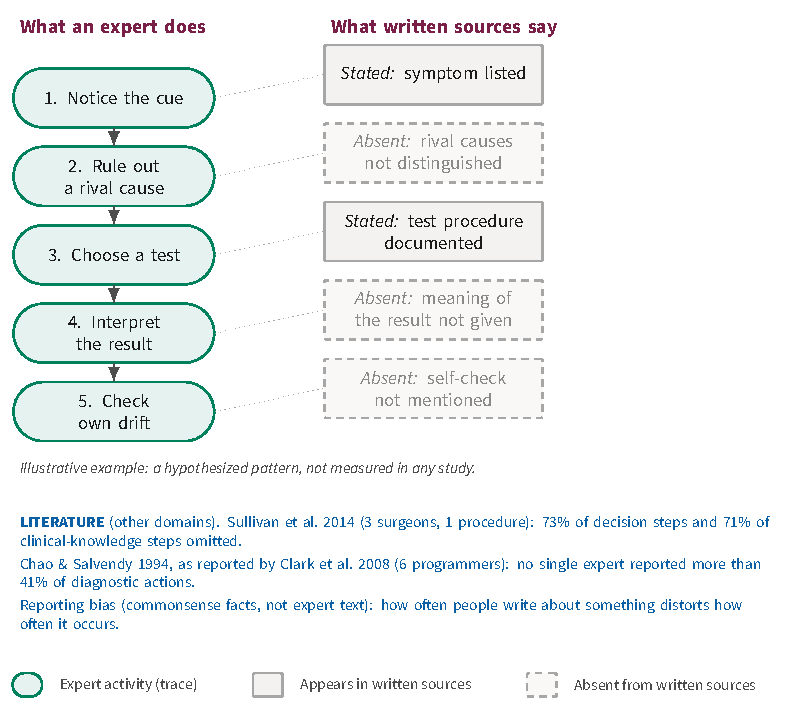
\includegraphics{figures/pdf/fig01_problem.pdf}
  \caption[What reaches text, and what does not]{What part of expert
    knowledge reaches text, and what does not. Automaticity, measured
    omission in three small studies, and reporting bias in written text
    explain why the overlap between ``what an expert knows'' and ``what an
    expert or a writer states'' is partial, and concentrated away from
    decisions, cues and interpretations.}
  \label{fig:problem}
\end{figure}

\subsection{Reporting bias: writers omit the obvious too}

\evlit\ Writers omit the obvious too: how often people write about actions,
outcomes and properties systematically distorts how often they occur
\parencite{gordon2013reporting}. Text-only language models inherit the
distortion, for example in the colors they predict for 521 objects
\parencite{paik2021world}. \evint\ Omission in speech and
reporting bias in text point at the same target: cues, decisions,
interpretations, checks and the boundaries of hedged rules, not the parts of
a domain already stated as principles or procedures.

\subsection{One education example: principle selection}

\evlit\ Experts sort physics problems by the principle that solves them
(conservation of energy, Newton's second law); novices sort the same
problems by surface features such as ``inclined-plane problems''
\parencite{chi1981categorization}. Naming the governing principle is an
expert operation that an expert does not think to state, because for the
expert it happens as recognition, not as a step. Experts do not just omit
their own principle-selection step; in the blind-spot studies reviewed in
\cref{sec:foundations-learners}, their predictions of what novices find hard
were well above chance but far from complete, and more expertise did not
improve them. Hence the education path
(\cref{sec:education}) never treats an expert's or an AI's guess about
learner difficulty as evidence.

\subsection{One organizational example: the copier technician's story}

\begin{evlitbox}
  Orr's ethnography of photocopier repair technicians found that diagnosis
  runs through narrative: technicians build and circulate a coherent story
  of how a machine is actually failing. That story, not the service
  manual, keeps the group's diagnostic knowledge current
  \parencite{orr1996talking}. Brown and Duguid read it as knowledge held by a
  community of practice \parencite{brown1991organizational}.
\end{evlitbox}

The manual describes the machine as designed; the technicians' story
describes it as it fails. \evobs\ Run on public troubleshooting text for
programmable logic controllers, the N3 gap map produced a record of the same
shape from the span ``a common mistake\dots\ is panicking and abandoning
systematic approaches.'' The sources name the failure mode, and the absence
check found at most a partial statement of how a troubleshooter notices the
drift into it (state: \code{partial}).\footnote{%
  \repo{research/n3/plc/gapmap.json}, the GUARD-lens record at rank 9.}
This shows only that a lens can flag text of this \emph{shape}; nothing
confirms that the item is real tacit knowledge, and the absence check is not
yet informative (\cref{sec:n3}).

\subsection{Why this matters}

The omission that makes a domain hard to teach also makes it expensive to
transfer inside an organization. \evlit\ Transfer of best practice
inside firms is blocked mainly by the recipient's capacity to absorb it and
by causal ambiguity, not by unwillingness to share
\parencite{szulanski1996exploring}. Software engineering shows what this costs when a
person who holds the knowledge leaves: many popular open-source projects
depend on one or two developers \parencite{avelino2016novel}. Turnover then
exposes projects to losses far above the expected loss
\parencite{rigby2016quantifying,nassif2017revisiting}
(\cref{sec:organizations}). \evint\ Training, onboarding and succession all
fail when such knowledge is not made explicit before its holder leaves.

\subsection{What AI changes, and what it does not}

An AI system can read far more sources than a person and keep a checkable
link from each claim to its supporting sentence (\cref{sec:approach}).
\evint\ What it cannot do is see past the wall the omission
and reporting-bias evidence describes: a language model trained on text
inherits the silences of that text \parencite{paik2021world}. An AI system
can make the boundary between what is written and what is not sharper and
more auditable, and it can flag the shape of a likely silence using the
constructs in \cref{sec:foundations}. It cannot tell on its own whether a
flagged silence hides real expert knowledge, a fact nobody happened to write
down, or nothing. That needs a human answer, which is why every output of
the pipeline carries an evidence label (\cref{sec:evidence-model}) and why
\code{inferred} never reads as \code{observed_human_evidence}.

\section{Research question and hypotheses}
\label{sec:question}

\Cref{sec:problem} established the premise: a domain reconstructed from public text is thin in
predictable ways. This section turns it into a testable question, three hypotheses and a falsifier.

\begin{keyquestionbox}
  \textbf{RQ-B.} Can AI reconstruct what is written about a domain, and predict where its own
  reconstruction is thin, so that the location of the human knowledge residual is identified before
  any human is asked?
\end{keyquestionbox}

RQ-B is the reoriented project's central question (\repo{REORIENTATION.md}, \S1, \S22). It asks
whether the \emph{same} system that reconstructs a domain can say where the reconstruction is
weakest, in a way that lines up with where a competent human would add something. \evint{} A
\enquote{no} would not make reconstruction worthless; it would mean targeting adds nothing over
asking experts everything, or over simpler signals such as text density.

\subsection{Hypotheses}

\paragraph{H1 --- Evidence reconstruction with provenance is feasible and checkable.} A system can
extract atomic claims from public sources and tie every evidence item to the exact span it came
from. It labels each claim's evidence status; claims without a locatable span stay labeled
\code{synthetic_extrapolation} and never act as a criterion. These links are checked rather than
trusted. H1 includes an adversarial part: gating the reconstruction lets fewer planted
falsehoods and fewer false answers through than the ungated model.

\paragraph{H2 --- Methodology lenses plus an absence check predict the human residual better than
the strongest baseline.} Constructs from cognitive task analysis and related methods
(\cref{sec:foundations}) are applied as lenses over the reconstructed evidence. Each lens firing is
followed by a check of whether the element the lens expects is stated there (the absence check,
\emph{closure} in the code). Together they rank areas by where an expert would add something the
evidence lacks. They do so better than the strongest baseline without this machinery, such as text
density or a plain language-model guess.

\paragraph{H3 --- Prioritized questions reduce expert time.} Questions chosen from the gap map
recover at least 1.25 times as many validated, previously unwritten items per expert hour as an
untargeted interview of equal length. The 1.25 is the smallest effect of interest (SESOI), fixed
before data, and a null result counts against H3. The PoC's breadth ranking and selection by expected information gain (not built)
are tested as separate selectors (\cref{sec:validation}, V6).

\evint{} H2 is the central hypothesis; \repo{REORIENTATION.md} and the program notes call it
\enquote{H1}. The order is one of dependency: H2 means something only if H1 holds, and H3 only if
H2's ranking beats chance. A negative result at one link does not falsify the link below it.

\subsection{The falsifier}

\begin{evfutbox}
  H2 is falsified if the upper bound of a 90\% confidence interval on $\Delta$AUROC falls below
  a SESOI $\delta$, fixed before any gold is acquired. $\Delta$AUROC is the gap map's area-level
  AUROC for ranking residual-present areas above others, minus that of the strongest
  pre-registered baseline. The
  blind prospective study (V5) reads this rule and decides H2. It has not run.
\end{evfutbox}

The gap map must beat its strongest competitor by at least $\delta$, not just chance. The test can
show that this margin is absent only when enough areas exist: about 150 per class for
$\delta = 0.05$. A single CTA gold gives perhaps 15--25 areas and cannot. \Cref{sec:validation}
therefore splits the work. A retrospective study pooled over several published CTA golds
\emph{screens} the gap map and releases money for the prospective study only if the map looks
promising. The prospective study is sized for about 150 areas per class and \emph{decides} H2.
Before either, a closure study tests whether the absence check works at all; it needs no grant.

\evhyp{} One further hypothesis sits outside this chain. \textbf{H-OSS:} the gap map, adapted to
code and commit evidence, predicts where knowledge is lost when developers leave. It concerns
organizational artifacts, not the human residual, so its result can neither support nor refute
H2.

No hypothesis has yet been tested against a human criterion (\cref{tab:hypothesis-status}).

\begin{table}[htbp]
  \centering\small
  \caption{What the zero-participant PoC could test for each hypothesis, and its status after N2 and
    N3. No cell reports a result against human knowledge.}
  \label{tab:hypothesis-status}
  \begin{tabularx}{\linewidth}{@{}p{0.05\linewidth}>{\raggedright\arraybackslash}p{0.33\linewidth}
      >{\raggedright\arraybackslash}X@{}}
    \toprule
    Hyp. & What the PoC could test & Status after the PoC \\
    \midrule
    H1 & Whether a pipeline with a claim ledger, verbatim provenance and cross-model verification
      runs end to end on real sources. &
      \evobs\ Engineering part: yes (\cref{sec:n2}). Adversarial part: N2's registered verdict is
      INCONCLUSIVE; E-PLANT's Continue branch closed on the validity floor, and the gated arms were
      never scored. \\
    H2 & Whether lenses fire on real text and whether the absence check separates \enquote{unstated}
      from \enquote{stated elsewhere}. &
      \evobs\ Mechanism only. Lenses fire on three ledgers; the judge's verdict does not depend on
      which evidence it is shown, so the absence check is not yet informative (\cref{sec:n3}). No
      $\Delta$AUROC has been computed. Next test: the closure study (V1), before any grant. \\
    H3 & Whether ranked questions can be produced at all. &
      \evfut\ Not tested. Template questions exist; no expert has answered one. \\
    \bottomrule
  \end{tabularx}
\end{table}

\section{Scientific foundations}
\label{sec:foundations}

This section surveys the traditions the methodology lenses (\cref{sec:n3})
are built from, and which part of the system each supports
(\cref{tab:methods}, \cref{fig:lenses}). \evint\ The literature supports the
\emph{constructs} each lens uses: a discrimination, a rival cause, a hedged
rule and its exception, a causal-ambiguity gap. It does not support the
lenses. No study cited here tests whether a detector built on these
constructs finds real expert knowledge in text. That test is what Part III is for.

\begin{figure}[!b]
  \centering
  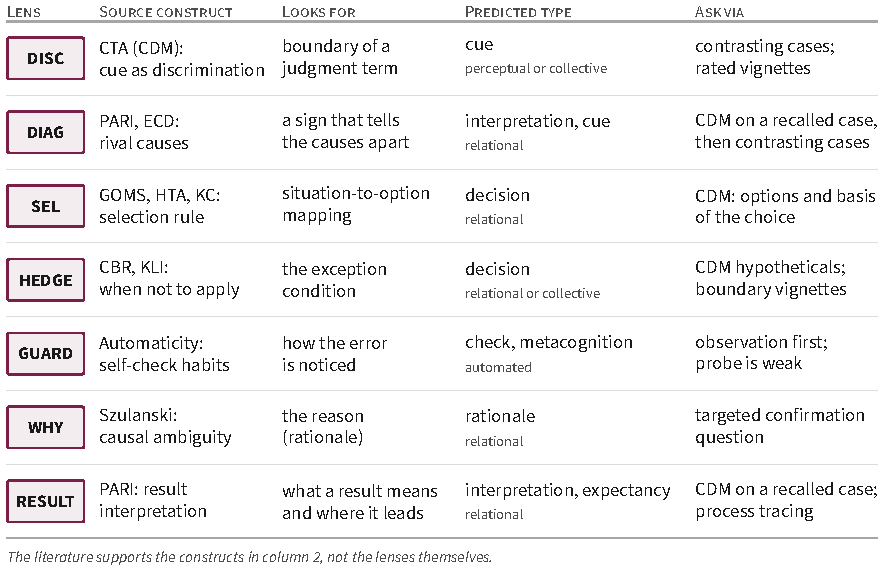
\includegraphics{figures/pdf/fig03_lenses.pdf}
  \caption[Which methodology gives which lens]{Which research method gives
    which methodology lens, and what missing element each lens looks for.
    Every arrow is a construct taken from the literature in this section;
    none of the lenses has been validated against a human judgment of where
    expert knowledge is missing (\cref{tab:methods}).}
  \label{fig:lenses}
\end{figure}

\subsection{Decoding the Disciplines: the bottleneck as framing}

Decoding the Disciplines (DtD) asks instructors to find a bottleneck where many students get stuck.
A ``decoding interview'' uncovers what experts do there; the instructor then models the step, gives
practice and feedback, and assesses it \parencite{middendorf2004decoding,pace2017decoding,pace2021beyond}.
\evlit\ The strongest controlled comparison we found favored DtD on hypotheses, operational
definitions and variables \parencite{pinnow2016decoding}. It covered introductory psychology, with 46
DtD and 45 control students. We found no randomized trial, no
controlled physics study and no retention or transfer measure. \evint\ The bottleneck idea frames which gap-map questions matter for
teaching and, with the model--practice--assess steps, the education path (\cref{sec:education}); the
decoding interview is not used as evidence (\cref{sec:investigated-not-central}).

\subsection{Cognitive task analysis, the Critical Decision Method and PARI}

Cognitive task analysis (CTA) is a family of more than 100 named methods
\parencite{yates2011advancing} for capturing the knowledge, decisions and
cues behind skilled performance
\parencite{schraagen2000cognitive,crandall2006working,clark2008cognitive}.
Its omission numbers are in \cref{sec:problem}. \evlit\ Here what matters is
what CTA-derived knowledge is \emph{worth} once recovered. A
meta-analysis of a small number of studies found CTA-based instruction
outperforms other ways of identifying training content, Hedges'
$g = 0.871$, varying substantially by method and context
\parencite{tofelgrehl2013cognitive}. In surgical training, a 12-study review
found standardized mean differences of 1.36 (95\% confidence interval, CI, 0.67--2.05) for
procedural knowledge and 2.06 (1.17--2.96) for technical performance
\parencite{edwards2021cognitive}. In an undergraduate biology course
(N~=~314, double-blind), CTA-derived instruction cut withdrawal from 8.1\% to
1.4\% of initial enrollment, against an award-winning instructor
\parencite{feldon2010translating}. Interviews with 52 scientists and
engineers yielded 29 problem-solving decisions shared across fields
\parencite{price2021detailed}.

\evint\ The schema's knowledge types (decision, cue, interpretation, check,
expectancy) are CTA categories. Pooling experts recovers more than any one
expert, so future gold standards are a union of experts plus a behavioral
trace. Published CTA task lists are candidate gold for the retrospective
study (\cref{sec:validation}). The thin but positive instructional evidence
is the basis for the education path.

\paragraph{The Critical Decision Method (CDM).} CDM works over one real,
recalled incident in several passes: a timeline, deepening probes, then
``what if'' questions \parencite{hoffman1998use}. It extends the
critical-incident technique with probes for perceptual and conceptual
discriminations, typicality judgments and critical cues
\parencite{klein1989critical}; ACTA is a streamlined practitioner version
\parencite{militello1998applied}. \evint\ CDM's probe for discriminations and typicality is the construct
behind the DISC lens, which fires when sources use a judgment term (``high
risk,'' ``abnormal'') without stating its boundary. CDM's other probes give
the human channel for DIAG, SEL, HEDGE and RESULT. Its question discipline is
the rule every lens's questions follow: retrospective, anchored to a real
incident, no yes/no questions, one construct per question.

\paragraph{PARI.} PARI (Precursor, Action, Result, Interpretation) was built
for U.S. Air Force troubleshooting training. For each step it records why the
action was taken, the action, its result, and what the result means for the
fault hypothesis \parencite{hall1995procedural}. It reports no outcome
statistics. Interpretation is where pooled expert coverage stayed lowest in
the programming study of \cref{sec:problem}. \evint\ PARI's
result-to-interpretation step is the construct behind the RESULT lens, which
fires when sources prescribe a test or check but never say which result maps
to which action. Joined with Evidence-Centered Design's alternative
explanations (below), the same step gives DIAG its construct: rival causes of
one effect with no sign in the text that separates them.

\subsection{Expert--novice differences}

\evlit\ In sorting tasks and think-aloud protocols, experts categorized
physics problems by the principle that solves them and novices by surface
features \parencite{chi1981categorization}. Experts recognize patterns and
chunks that guide them \parencite{larkin1980expert,chase1973perception}.
Perceptual expertise can
be taught directly. In chick sexing, naive participants given a short
instruction on one shape contrast rose from near-chance to expert-level
accuracy. Their item-level agreement with experts rose from a correlation of
.21 to .82 \parencite{biederman1987sexing}. \evint\ A
perceptual cue is therefore a discrimination that contrasting cases can
teach, which is why DISC's human channel routes to contrasting-case
classification and not to interviews alone. The knowledge type
\code{expert_novice_contrast} and the planned bottleneck-hypothesis object
(``expert has, novice lacks, novice substitutes'') come from this work.

\subsection{What experts misjudge about learners}
\label{sec:foundations-learners}

\begin{evlitbox}
  Three blind-spot findings, each at its own grain. Among 48 preservice
  secondary teachers, those with more advanced mathematics
  education were more likely to treat symbolic equations as a prerequisite
  for word and story problems, the reverse of students' actual performance
  pattern \parencite{nathan2003expert}. In two studies, one with expertise
  experimentally manipulated, participants with more expertise predicted
  novice task-completion times worse and resisted debiasing; intermediates
  may be the more accurate predictors \parencite{hinds1999curse}. In a physics study, 25
  first-year physics graduate teaching assistants (TAs) and 30 physics
  instructors predicted introductory students' most common wrong answer on
  each Force Concept Inventory item. The TAs scored 65\% of the maximum
  possible score and the instructors 68\%, against 40\% for random guessing.
  Both groups beat random guessing, and they did not differ significantly
  from each other \parencite{maries2016teaching}.
\end{evlitbox}

\evint\ The pattern recurs across settings, but it is not a general law that
misjudgment grows with expertise. The variable is mathematics coursework in
one study and experimentally induced expertise in another. In the physics
study, the instructors' greater teaching experience did not help. What the findings license is
narrower and sufficient here: expert judgment of learner difficulty is not
reliable evidence of it.

\paragraph{Pedagogical content knowledge (PCK).} Shulman named the knowledge
teachers need beyond subject matter: how to represent a topic, and what
makes it easy or hard for learners, including their preconceptions
\parencite{shulman1986those,shulman1987knowledge}. \evlit\ Across 9,556
students of 181 middle-school teachers, teachers who could identify a popular
wrong answer produced larger gains on the affected items than teachers who
knew only the right answer \parencite{sadler2013influence}. PCK names the
layer the gap map does not reach: knowledge about learners, not about the
domain.

\paragraph{Threshold concepts and conceptual change.} A threshold concept
opens ``a new way'' of seeing a subject and is often ``troublesome'':
counter-intuitive or alien to the learner
\parencite{meyer2003threshold,meyer2005threshold,meyer2006overcoming}; the
framework is conceptual, not an effect size. Research on conceptual change
asks how learners restructure prior ideas. The classical model needs
dissatisfaction and an intelligible, plausible, fruitful replacement
\parencite{posner1982accommodation}. ``Knowledge in pieces'' instead treats
intuitive physics as many small context-bound elements
\parencite{disessa1993toward}, and misconceptions as knowledge in transition
\parencite{smith1994misconceptions}. \evlit\ The Force Concept Inventory
builds its wrong-answer options from common beliefs about force and motion
\parencite{hestenes1992force}, and bug libraries model procedural errors as
systematic ``bugs'' in an otherwise correct procedure
\parencite{brown1978diagnostic}.

\paragraph{What this contributes.} These findings constrain the design. The
GUARD lens never asserts that a learner will find something difficult, only
that sources report guarding against an error. Learner difficulty is a
separate layer, established only from learner response data (concept
inventories are candidate gold in physics); \code{misconception} is stored as
a hypothesis with its evidence, neutral between the classical and
knowledge-in-pieces views. No lens derives from threshold concepts, because
identifying one relies on the expert judgment the blind-spot evidence calls
into question.

\subsection{Tacit knowledge: Polanyi and Collins}

Tacit knowledge is knowledge people use but do not, or cannot, put into
words: ``we can know more than we can tell'' \parencite{polanyi1966tacit}.
Collins divides it into \emph{relational} (unsaid for contingent reasons,
explicable if someone bothered), \emph{somatic} (tied to the body, so that
explaining it does not confer the skill) and \emph{collective} (held in
social practice) \parencite{collins2010tacit}. These, plus \code{automated} and
\code{perceptual}, are the system's tacitness labels, assigned by rule as an
\code{inferred} prediction. \evint\ Relational knowledge is the part a gap map
can hope to predict and a question can hope to recover. Somatic and
collective knowledge need observation or presence in a community of
practice; the system does not claim to reach them.

\subsection{Organizational knowledge: SECI and causal ambiguity}

Nonaka's SECI model proposes four modes by which tacit knowledge becomes
explicit in an organization: socialization, externalization, combination and
internalization \parencite{nonaka1994dynamic}. \evlit\ A critical review
judges it ``flawed'': three of its four modes appear plausible, but none of
the four is supported by evidence that a simpler account cannot explain, and
the model omits knowledge that is inherently tacit
\parencite{gourlay2006conceptualizing}. A study of 271
observations of 122 best-practice transfers in eight companies found the main
barriers knowledge-related, not the source's unwillingness to share
\parencite{szulanski1996exploring}. They were the recipient's limited
absorptive capacity, causal ambiguity about why the practice works, and an
arduous relationship between source and recipient.

\evint\ Causal ambiguity is the construct behind the WHY lens: a prohibition
or contrasting instruction that sources prescribe without its reason. The
organizational application (\cref{sec:organizations}) targets missing
rationale first, as a hypothesis. Given the critique, this report never reads
SECI's ``externalization'' as evidence that tacit knowledge can be made
explicit on demand.

\subsection{Reporting bias in text}

People do not write down what is obvious to them, so a fact's frequency in
text does not track its frequency in the world; the two supporting results
\parencite{gordon2013reporting,paik2021world} are given in \cref{sec:problem}.
\evint\ Reporting bias bridges CTA (experts omit the obvious when they
\emph{talk}) and reconstruction from text (writers omit it when they
\emph{write}). Together they predict that the residual concentrates in cues,
expectancies and automated checks, which is why the lenses look for those
types rather than for sparsely covered topics in general. The lens design
applies one consequence, ``fire narrow, close wide'': a lens fires only on a
narrow pattern, while any retrieved ledger sentence, in any wording, may
close the gap. \evhyp\ Boundary-text density, how much text surrounds a
term's boundary without stating it, is a candidate ranking feature; it is
not implemented.

\subsection{Evidence-Centered Design and the Knowledge-Learning-Instruction
  framework}

Evidence-Centered Design (ECD) treats an assessment as an argument from what
a student does to a claim about what the student knows
\parencite{mislevy2003structure}. The Knowledge-Learning-Instruction (KLI)
framework uses the knowledge component (KC) as its unit, including the
condition under which it applies \parencite{koedinger2012knowledge}. \evint\ ECD's alternative explanations
for one observation give DIAG its construct. KLI's KC condition, the ``when,
and when not, to apply'' part, gives two lenses theirs. SEL fires on a named
selection criterion with no mapping from situation to option. HEDGE fires on a
hedged rule with no stated exception. A planned layer would store KCs with
their conditions; it is not built, and KC models are ordinarily validated
against learner data, which the zero-participant PoC does not have.

\subsection{Knowledge elicitation, requirements engineering and underspecified text}

The knowledge-engineering tradition behind expert systems studied which
elicitation techniques recover which kind of knowledge
\parencite{cooke1994varieties,hoffman1995eliciting}. Its families are
observation and interviews, process tracing, and conceptual techniques such as
sorting and repertory grids.
\evlit\ Task, method and number of experts all changed what was recovered in
the programming study of \cref{sec:problem} \parencite{chao1994percentage}.
\evint\ This is the basis for the rule that a gap's predicted knowledge type
decides its human channel (a CDM probe, a contrasting-case task, or
observation first for automated skills). The full type-to-channel mapping is
our synthesis, not a validated table.

\evlit\ Requirements engineering already detects incompleteness in text and
treats tacit knowledge as something to surface. A completeness assistant
compares a specification with its input documents and points out relevant
terms and relations the specification lacks \parencite{ferrari2014measuring}.
Masked-language-model predictions flag terminology missing from
requirements; they were tested by withholding parts of 40 specifications
\parencite{luitel2024improving}. In 34 customer--analyst interviews,
ambiguity turned out to be a resource for discovering tacit knowledge, not
only an obstacle \parencite{ferrari2016ambiguity}
\parencite[see also][]{gervasi2013unpacking}. Closest to our lenses,
\textcite{torre2020ai} check privacy policies under the EU General Data Protection
Regulation (GDPR) for \emph{typed} content.
A conceptual model lists the information the regulation requires; a
classifier labels each policy's content; a completeness check reports the
required types that are absent. On 24 unseen policies it found 45 of 47
incompleteness issues, with eight false positives. This is construct-driven
absence detection, in one of the PoC's own domains.

\evlit\ Natural-language processing (NLP) studies the same silence in
instructional text. \textcite{anthonio2020wikihowtoimprove} built a corpus of
revision histories for about 2.7 million wikiHow sentences, to ask whether
edits add clarifications needed to follow an instruction.
\textcite{anthonio2022clarifying} extract implicit and underspecified phrases
from those histories, with the human clarifications that later resolved
them. Their gold for \enquote{what the text left unsaid} is a later human
edit.

\evint\ Together these are the nearest precedent for lenses as absence
detectors, and they narrow what may be new here. They work on one document
or one interview. Their reference is a regulation, an input document or a
later edit, which already contains or reveals the missing content. The
missing types come from that reference, not from constructs of expertise
research. None predicts what practitioners know beyond all the written
sources, or routes a gap to an elicitation channel.

\small
\begin{longtable}{@{}p{0.15\linewidth}p{0.24\linewidth}p{0.26\linewidth}p{0.24\linewidth}@{}}
  \caption{Methodology, the construct it supplies, the system component built
    from it, and the evidence status of that construct as used here. Every
    lens output carries the evidence label \code{inferred}; nothing in this
    table upgrades that label.}
  \label{tab:methods} \\
  \toprule
  Methodology & Construct used & System component & Evidence status \\
  \midrule
  \endfirsthead
  \multicolumn{4}{l}{\tablename\ \thetable{} -- continued from previous page} \\
  \toprule
  Methodology & Construct used & System component & Evidence status \\
  \midrule
  \endhead
  \midrule
  \multicolumn{4}{r}{Continued on next page} \\
  \endfoot
  \bottomrule
  \endlastfoot
    CTA & Experts omit decisions, cues, interpretations &
      Knowledge types decision/cue/interpretation/check/expectancy; premise
      of the gap map &
      Omission established in direction; rates small-$n$, one domain each \\
    CTA-based instruction & Recovered expert knowledge improves teaching &
      Education path &
      Positive in direction; few, small studies; no transfer outcomes \\
    CDM & Discriminations, typicality, incident-based probes &
      DISC lens; question rules for every lens; channel for DIAG, SEL,
      HEDGE, RESULT &
      Method established; no validation of this lens use \\
    PARI & Result$\to$interpretation step &
      RESULT lens; DIAG lens &
      Method documented (1995 guide); lens unvalidated \\
    Expert--novice & Principle vs.\ surface representation &
      \code{expert_novice_contrast} type; education path &
      Established \\
    Expert blind spot & Experts misjudge learner difficulty &
      GUARD lens restriction; learner data as the only gold for difficulty &
      Recurs across settings; small samples; no general expertise gradient \\
    PCK & Knowledge of learners' difficulties &
      Education path; separate learner-difficulty layer &
      Construct established \\
    Threshold concepts & Transformative, troublesome concepts &
      Education-path prioritization &
      Hypothesis; identification relies on expert judgment \\
    Conceptual change & Misconception as a context-bound hypothesis &
      \code{misconception} type stored as a hypothesis; future physics gold &
      Live theoretical dispute \\
    Tacit knowledge & Relational / somatic / collective &
      Tacitness vocabulary; channel routing &
      Conceptual framework, not empirical \\
    Organizational knowledge & Causal ambiguity blocks transfer &
      WHY lens; organizational path &
      One large study (271 observations); SECI judged flawed \\
    Reporting bias & Text omits the obvious &
      Gap-map prior feature (planned); ``fire narrow, close wide'' &
      Shown for commonsense facts; size in expert text unmeasured \\
    ECD & Alternative explanations of one observation &
      DIAG lens; bottleneck-hypothesis object (future) &
      Framework established; mapping is interpretation \\
    KLI & Knowledge component with a condition &
      SEL lens; HEDGE lens; future layer L2 &
      Framework established; mapping is interpretation \\
    Knowledge elicitation & Technique fits knowledge type &
      Type$\to$channel table for each lens &
      Taxonomy established; full mapping is our synthesis \\
    Requirements engineering & Incompleteness and tacit knowledge detectable from text or interview cues &
      No component; nearest precedent for the lenses &
      Detection shown against a reference, including regulation-typed completeness checking; not
      expertise-construct based, not routed \\
    Underspecification in instructional text & Later human edits reveal what text left implicit &
      No component; precedent for absence detection in how-to text &
      Corpora and models shown; phrase-level, gold from edits \\
    DtD & Bottleneck &
      Question framing only &
      Low to moderate; decoding interview not evidential \\
\end{longtable}

\subsection{Investigated but not central}
\label{sec:investigated-not-central}

An earlier design made DtD's decoding interview the validity anchor for
elicitation. This was falsified: the decoding interview has never been
compared with another elicitation method in a controlled way, and the CTA
evidence is stronger (\repo{research/falsify-decoding-the-disciplines.md}).
\evint\ What survived is narrower: locating a bottleneck from real student
data, modeling the step with practice and feedback, and assessing it, used as
the teaching frame in \cref{sec:education}. Four other lines were examined
and set aside for the NOW program. Bayesian knowledge tracing models mastery
from graded responses \parencite{corbett1995knowledge} and needs learner data
the program does not have. Intelligent tutoring systems show a median effect
of 0.66 standard deviations over 50 evaluations
\parencite{kulik2016effectiveness}, but they evaluate a delivery channel and
say nothing about what text omits. Knowledge Space Theory models feasible
knowledge states and learning order \parencite{doignon1985spaces} and waits
for learner data. A brief decision-based physics intervention (N~=~390,
quasi-experimental) had no direct effect on performance
\parencite{jeong2024effects}, a caution that making expert decisions explicit
is not enough on its own. \evlit\ Finally, large language model (LLM) personas matched real survey
respondents' average scores but showed much less variation. Regression
coefficients from synthetic responses often differed from those on the real
survey \parencite{bisbee2024synthetic}. This is the direct evidence behind
the rule that synthetic output may be a predictor, never a criterion, and
never feeds a gate.

% report/sections/04_approach.tex -- Part I: synthesis of existing methods into the proposed approach.
\section{From existing methods to the proposed approach}\label{sec:approach}

Five research traditions each solve part of our problem. None answers the question this project
asks: \emph{in this domain, where does the written record stop, and what kind of knowledge is likely
to lie beyond it?} The methods themselves are in \cref{sec:foundations}.

\subsection{What each tradition does well, and where it stops}\label{sec:approach-traditions}

\paragraph{Cognitive task analysis} \evlit{} reaches the decisions, cues and interpretations experts
skip \parencite{schraagen2000cognitive,klein1989critical,hall1995procedural}. \evint{} Every answer
costs expert time, pooling experts multiplies it \parencite{chao1994percentage}, and CTA starts
from the expert, not the written record, so it cannot say where the first interview hour is best
spent.

\begin{figure}[!b]
  \centering
  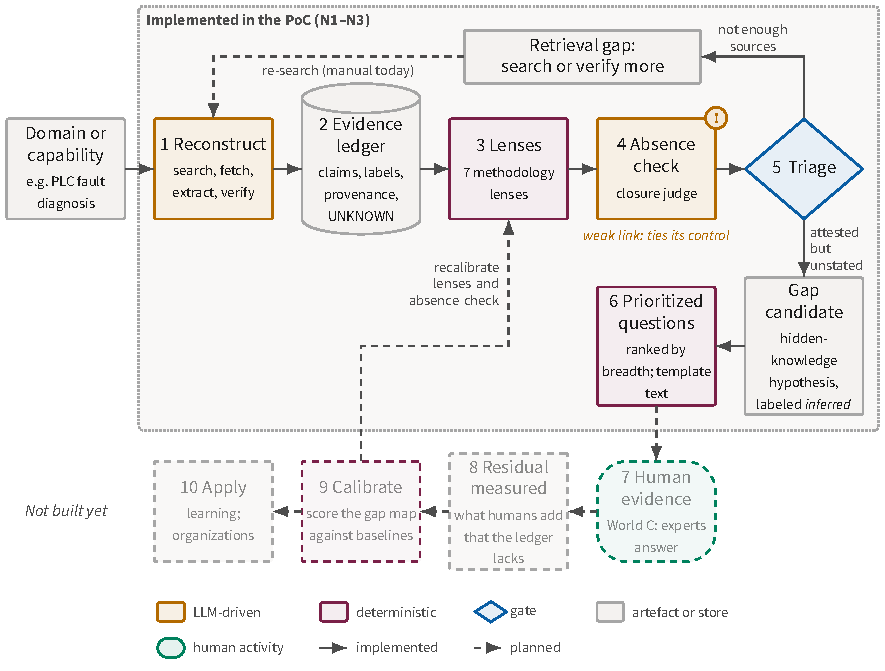
\includegraphics{figures/pdf/fig02_model.pdf}
  \caption[The central model]{What is the whole approach, and which parts exist today? A domain or
    capability enters at the top. Steps 1--6 (solid) are implemented in the PoC: reconstruction,
    evidence ledger, methodology lenses, absence check, triage and questions. Steps 7--9 (dashed)
    are future work: human evidence, calibration and application. Triage splits the output into two
    kinds of gap. A retrieval gap is listed for further search; in the PoC that is a manual re-run,
    since no code feeds it back to reconstruction. Only a gap candidate becomes a hidden-knowledge
    hypothesis (labeled \emph{inferred}) and an expert question. The absence check (step 4) is the
    weak link in the PoC.}
  \label{fig:model}
\end{figure}

\paragraph{LLM research tools} \evlit{} write cited syntheses
\parencite{shao2024assisting,skarlinski2024language,asai2024openscholar} and check atomic claims
against sources \parencite{min2023factscore,rashkin2023measuring,gao2023enabling}, but inherit the
reporting bias of text \parencite{gordon2013reporting,paik2021world}, and their citations often do
not fully support the statements \parencite{liu2023evaluating,venkit2025deeptrace,wu2025automated}.
\evint{} A cited synthesis has no place to record \enquote{searched and found nothing}.

\paragraph{Knowledge management} \evlit{} separates tacit from explicit knowledge
\parencite{nonaka1994dynamic} and codifying from connecting people \parencite{hansen1999whats};
\evint{} the split is a category or a strategy, not a measurement per task.

\paragraph{Requirements engineering and instructional-text NLP} \evlit{} flag terms and relations a
specification lacks relative to its inputs \parencite{ferrari2014measuring}. They predict likely
omissions with a masked language model \parencite{luitel2024improving} and use interview ambiguity as
a cue to tacit knowledge \parencite{ferrari2016ambiguity}. \textcite{torre2020ai} check GDPR privacy policies
against a conceptual model of the content the regulation requires, and report which required types
are absent. NLP work on wikiHow finds implicit and underspecified phrases, with later human edits as
gold \parencite{anthonio2020wikihowtoimprove,anthonio2022clarifying}. \evint{} Each works on one
document or interview against a reference that fixes the missing types in advance. None predicts
knowledge held only by practitioners or routes it to an elicitation channel.

\paragraph{Gap finding in literature} \evlit{} maps \enquote{structured absences} in papers
\parencite{ono2026mapping}, implicit gaps in biomedical literature \parencite{salem2025gapmap} and
knowledge-base completeness \parencite{razniewski2024completeness}. These are research unknowns, not
knowledge practitioners hold. Our \code{gapmap} package shares only a name with
\textcite{salem2025gapmap}.

\paragraph{The synthesis.} \evint{} We add to reconstruction with provenance a record of what was
searched and not found. We run expertise constructs as detectors over it. And we turn the
codified/personal split into a quantity measurable in principle per task area: the Human Knowledge
Residual (HKR, \cref{sec:residual}). It is a research construct, not an observed quantity.

\subsection{The central model}\label{sec:approach-model}

\Cref{fig:model} shows the approach; steps 1--6 are built in the proof of concept (PoC), 7--9 are
not (implementation: \cref{sec:architecture}; lenses and absence check: \cref{sec:n3}).


\begin{description}[style=nextline, leftmargin=1.5em, itemsep=1pt]
  \item[1 Reconstruct] Fetch public (World~A) sources, extract claims, locate each quote in a hashed
    snapshot, verify it with a model of another family (\cref{sec:n2}).
  \item[2 Evidence ledger] Claims with one of six epistemic labels. Located claims carry an exact
    span; extractions whose quote cannot be located stay labeled \code{synthetic_extrapolation} and
    never act as a criterion. \code{unknown} marks a slot searched and not covered
    (\cref{sec:evidence-model}).
  \item[3 Lenses] Seven lenses, one construct each (\cref{fig:lenses}), \emph{fire} when sources
    attest a construct but not its content, e.g.\ rival causes with no sign that separates them.
    They read the extractor's paraphrase of each claim, not the verbatim span (\cref{sec:n3}).
  \item[4 Absence check] A judge model reads the sentences a lexical retriever pulls from the ledger
    (up to 8 verified and 4 unverified per probe) and returns \emph{closed}, \emph{partial} or
    \emph{open}; closed firings are dropped.
  \item[5 Triage] A \textbf{retrieval gap} (searched and not found, one independent source,
    unverified text only, answered by a sibling run, or an unreadable verdict) calls for search,
    verification or re-judging, not an expert. A \textbf{gap candidate} has at least two independent
    sources on the attested side, and the absence check did not mark the missing element as fully
    stated. Most displayed PoC candidates are partial: the lens fired, and the absence check found
    the element at most partly stated (\cref{sec:n3}). It becomes a three-tier
    record: observed evidence, inferred gap, hypothesis labeled \emph{inferred}.
  \item[6 Questions] Template-filled (no model writes them), with a predicted knowledge type and a
    human channel; ranked by a breadth rubric, not expected information gain (future work, N6).
  \item[7--9 Future] Expert answers (World~C) measure the residual, score and recalibrate the gap
    map, and only then feed instruction or organizational uses.
\end{description}

\evhyp{} The mechanism serves one hypothesis (H2, \cref{sec:question}). Suppose a lens fires, a
working absence check does not find the missing element stated, and the attested side has broad
support. Then practitioners are more likely there than elsewhere to hold knowledge the text lacks. The PoC builds the
mechanism; it does not test the hypothesis.


\begin{evobsbox}
  The absence check did not beat its mismatched-evidence control. The control keeps each candidate's
  seed in both arms and swaps its other-source evidence for a neighbor's. Under this control the judge
  did not tell the candidate's own cross-source evidence from the neighbor's, so it is not yet an
  informative absence check (\cref{sec:n3,sec:interpretation}).
\end{evobsbox}

\begin{table}[!tbp]
  \centering
  \footnotesize
  \caption[Novelty ledger]{Novelty ledger: each element of the approach in one category, with its
    closest precedent. \emph{Adaptation}: a known idea on a new unit or purpose. \emph{Engineering
    contribution}: no research claim. \emph{Potentially novel}: no match found; \enquote{uncertain}
    where paywalled, unpublished or commercial work may overlap.}
  \label{tab:novelty}
  \begin{tabularx}{\linewidth}{@{}>{\raggedright\arraybackslash}p{0.32\linewidth}>{\raggedright\arraybackslash}p{0.2\linewidth}>{\raggedright\arraybackslash}X@{}}
    \toprule
    Element & Category & Precedent or reason \\
    \midrule
    Epistemic label per claim & Known method & Graded evidence and provenance typing \parencite{guyatt2008grade,lebo2013provo} \\
    Claim ledger: atomic claims, verbatim spans from hashed snapshots, verifier of another family & Known combination & \textcite{min2023factscore,rashkin2023measuring,sanderson2017web}; same quote re-check in \textcite{kassis2026mimeo} \\
    \code{unknown} only for a searched, uncovered slot & Adaptation & Abstention and completeness \parencite{wen2025know,razniewski2024completeness} \\
    Independence clustering, contradiction handling & Engineering contribution & Hygiene; no research claim \\
    Planted-falsehood and abstention harnesses (N2) & Adaptation & \textcite{wu2024clasheval,kirichenko2025abstentionbench}; N2 read inconclusive \\
    Methodology lenses as absence detectors over a provenance ledger & Adaptation & Typed absence detection against a reference exists \parencite{torre2020ai}; also \textcite{anthonio2022clarifying,luitel2024improving,ferrari2016ambiguity,jin2026chat,shen2025requirements,salem2025gapmap}. New here only the source of the types (expertise constructs) and the target (knowledge beyond all sources). Validity not shown (absence check ties its control) \\
    Predicted knowledge type per candidate & Adaptation & Taxonomies exist \parencite{collins2010tacit,gervasi2013unpacking,klein1989critical} \\
    Elicitation channel chosen by knowledge type & Known method & \textcite{klein1989critical,gervasi2013unpacking,burton1990efficacy} \\
    Retrieval gaps routed to search, not to experts & Adaptation & Retrieve-or-ask split in \textcite{taranukhin2026infogatherer} \\
    Three-tier records, anti-renaming check, closure controls, cross-run check & Engineering contribution & Evaluation hygiene; the built-in mismatched-evidence control carries the closure failure that an adversarial review found \\
    Question priority by expected information gain & Known method (not built) & \textcite{lindley1956measure,rao2018learning,choudhury2025bedllm} \\
    Residual as a measurable quantity; unseen-item estimation & Adaptation & Estimators exist \parencite{chao1987estimating,chao2012coverage}; naming the residual is framing \\
    Residual lies in steps obvious to experts & Known combination & \textcite{gordon2013reporting,paik2021world,sullivan2014use,chao1994percentage} \\
    Synthetic output as predictor only, never criterion & Known method & Simulated samples as a proxy: \textcite{argyle2023out}; the limits that motivate the restriction: \textcite{bisbee2024synthetic,cui2025large} \\
    Gap map predicts where the residual lies (RQ-B, H2) & Research hypothesis & Untested; the PoC did not acquire gold \\
    Scoring a gap map against published CTA results (E-CTA) & Potentially novel, evaluation design (uncertain) & No such comparison found; gold sets are small (3--17 experts, one domain each) \\
    Developer departures as ground truth for a separate organizational hypothesis (E-OSS) & Adaptation & Turnover, quality and truck-factor work \parencite{foucault2015impact,rigby2016quantifying,avelino2016novel,nassif2017revisiting}; rationale mining from issue trackers \parencite{zhao2024drminer} \\
    Whole chain, domain-neutral, evidence status carried end to end & Potentially novel (uncertain) & No single system found; commercial tools may not publish methods \\
    \bottomrule
  \end{tabularx}
\end{table}

\subsection{Closest prior work, and what may be new}\label{sec:approach-closest}\label{sec:approach-novelty}

Our search covered peer-reviewed venues, arXiv and public product material, to September 2026. It
found precedent for every step. The closest work is closer than our first search showed, so we
state it first.
\begin{itemize}[nosep]
  \item \textcite{torre2020ai} check GDPR privacy policies for required content types taken from a
    conceptual model of the regulation. That is typed absence detection in one of our own domains.
    The types come from the regulation, and the reference fixes what should be present.
  \item \textcite{anthonio2022clarifying} find implicit and underspecified phrases in instructional
    text, with later human edits as gold. The gold is a later version of the same text, not
    knowledge held only by practitioners.
  \item DRMiner \parencite{zhao2024drminer} extracts design rationale from issue-tracker discussions,
    the kind of evidence our WHY lens would read in software. \textcite{foucault2015impact} measure
    the effect of developer turnover on quality in open-source projects. Both sit inside the
    literature our departure study (E-OSS) would join.
  \item \textcite{luitel2024improving} flag terms missing from a requirements document but do not
    type them or ask anyone. OntoAgent \parencite{jin2026chat} picks requirements-interview questions
    from an ontology, with no ledger and no prediction of where sources are silent.
  \item In PKAI \parencite{schinckus2025large} and GenAI-supported interviews \parencite{walther2026genai},
    as far as the abstracts show, no map of what documents lack drives the questions.
    \textcite{zuin2025leveraging} simulate the organization and its hidden knowledge. UQS
    \parencite{ono2026mapping} maps research unknowns and asks no experts.
\end{itemize}

\evint{} \Cref{tab:novelty} places each element in one category. Given this work, methodology lenses
as absence detectors are an adaptation, not a new idea. What we did not find is a method that chains
the parts the PoC chains:
a provenance ledger with an evidence status per claim, expertise constructs as typed absence
detectors over it, a knowledge type and human channel per suspected gap, and search failures kept
apart from expert questions. That combination is the most defensible claim, and only as a proof of
concept. The absence step did no better than a control, and whether the gap map predicts what experts
add is open (\cref{sec:validation}). The evaluation design that scores a gap map against published
CTA results is a stronger novelty candidate than the system, but it has not run.


% ---------------------------------------------------------------- Part II
\reportpart{The Proof of Concept}{What was built, what it produced, and
  what it does and does not show.}
\section{Scope of the proof of concept}
\label{sec:scope}

\subsection{What the PoC set out to show}

The proof of concept (PoC) had one narrow engineering goal: build a working, checkable chain
from a named domain or capability to a ranked list of questions for a human expert. It used only
public evidence, with zero participants at any step. \evobs{} \emph{Checkable} means three things.
First, every criterion-labeled claim's evidence is an exact, byte-identical span in a document the
system fetched itself. A claim the extractor could not ground this way stays in the ledger as
\code{synthetic\_extrapolation} and never acts as a criterion (\cref{sec:evidence-model}). Second,
every epistemic label is computed from that evidence rather than typed in by hand. Third, every
stage's tests run offline. The chain has four stages:
\begin{enumerate}[noitemsep]
  \item reconstruct a domain's written record with provenance (\cref{sec:architecture});
  \item keep that record as an explicit evidence ledger with six epistemic labels
    (\cref{sec:evidence-model});
  \item apply methodology lenses that ask whether a named construct's content is stated anywhere
    in the ledger; and
  \item rank the resulting candidates into expert questions.
\end{enumerate}
Each stage is implemented code, run on real web sources, with a committed test suite.

The PoC was not meant to show, and does not show, that the resulting questions or their ranking
point at what a real expert actually knows and the record does not. That is a separate claim
(RQ-B, \cref{sec:question}) that needs human evidence to test, and the PoC deliberately used none.
\evint{} What the PoC demonstrates is a mechanism: a chain that turns silence in the written
record into a labeled, ranked hypothesis. Whether that hypothesis is right is untested. The gap
map's own closure step does not yet beat a fair control (\cref{sec:n3,sec:not-demonstrated}), so
even the mechanism's central move is an open question, not a working result.

\subsection{Why zero participants}

The PoC was built entirely inside what \repo{REORIENTATION.md} (\S22) calls the NOW program:
zero participants, zero proprietary or customer data, zero microphones, and zero live expert
interviews. \evobs{} The one human input the program allows at all is a single blind second
coder, used for labeling rather than participation, and that step has not yet been exercised.
The constraint follows directly from the project's own history (\cref{sec:track-a-history}
below): every gate that needed a human to run first stalled on recruiting that human. A design
that needs no participant to reach its first checkable result can be built, tested, and revised
on the calendar of the engineering team alone. Its failures are attributable to the code and
the public evidence, not to a small or biased human sample. \evint{} The cost is symmetric: a
zero-participant PoC cannot, by construction, validate the one claim that matters most --- that
the reconstruction's thin spots correspond to what humans actually know. That validation is
future research (\cref{sec:not-demonstrated,sec:residual,sec:validation}), pre-registered before
any gold data is acquired.

\subsection{How the project reached this design}
\label{sec:track-a-history}

The project began as a physics-education study. Twelve physicists would be interviewed with an
AI-assisted think-aloud and retrospective-probe protocol, and about 370 first-year students would
sit a two-arm randomized trial with delayed transfer. Building the instrument for that study --- a
session app, a coding pipeline, five architecture decisions, and four rounds of lessons drained
into the codebase --- absorbed most of the project's effort. \evobs{} The instrument is complete
and tested: \repo{instrument/} runs 311 tests (\code{uv run --directory instrument pytest -q}).
Every one of its gates, though, from the first pilot session to the final randomized trial,
needed physicists, students, or both to exist before any result could be read.

A self-diagnosis in \repo{REORIENTATION.md} \S3 named this pattern \emph{drift}: a
falsification discipline that demanded validation against observed human performance had,
with no participants recruited yet, nowhere to go except building the instrument ever more
carefully. \evint{} Public-evidence reconstruction, organizational knowledge, and
evidence-grounded synthetic cohorts had never been considered as alternative first steps, so
work of that kind could not register as progress against the existing plan. The owner adopted a
reorientation on 2026-09-28 (\repo{REORIENTATION.md}, \S3, \S22). It freezes the physics study
and its instrument as \emph{Validation Track A}, unchanged and started only on its own registered
preconditions (experts, a course, ethics approval). It also opens a new, parallel program --- NOW,
items N0 through N9 --- whose every item can start and end without a single participant. N0--N3 are
built; \cref{tab:now-verdicts} (\cref{sec:evolution}) tracks what each one did and the verdict it
read. \Cref{tab:now-items} lists the six items that are not yet started.

\begin{table}[tbp]
  \centering
  \small
  \caption{The NOW program's not-yet-started items, N4--N9 (\repo{REORIENTATION.md}, \S22); N0--N3
  are tracked separately in \cref{tab:now-verdicts}. Every item, built or not, is pre-registered to
  end in a continue/change/stop reading of an experiment result, not in a build
  (\cref{sec:evolution}).}
  \label{tab:now-items}
  \begin{tabularx}{\linewidth}{@{}llX@{}}
    \toprule
    Item & Status & One line \\
    \midrule
    N4 & Not started & Behavioral validity: does the reconstructed model fit real learner
      responses? \\
    N5 & Not started & Residual measurement: estimate unseen items against gold as an
      independent occasion. \\
    N6 & Not started & Question selection by expected information gain against held-out gold. \\
    N7 & Not started & Evidence-grounded synthetic cohorts, validated in tiers, never a
      criterion. \\
    N8 & Not started & E-SEAL: sealed Track A predictions, secondary and non-gating. \\
    N9 & Not started & E-COST: a running ledger of cost per validated item. \\
    \bottomrule
  \end{tabularx}
\end{table}

This report covers N0--N3: the four items that exist. \evfut{} N4--N9 are described only as the
research program that would follow (\cref{sec:validation,sec:roadmap}); nothing under those
items has been built or run.

\section{Architecture of the implemented PoC}
\label{sec:architecture}

\subsection{Three packages, one direction}

The PoC is three independent Python packages, each built as its own \code{uv} project, connected
by a strict one-way dependency chain: \repo{residual/} $\rightarrow$ \repo{reconstruct/}
$\rightarrow$ \repo{gapmap/}. \evobs{} Within that chain, a package may import stdlib,
\code{pydantic}, and any package to its left, and nothing else. \repo{reconstruct/} also depends on
\code{httpx}, \code{openai}, \code{tldextract}, and \code{pypdf} for what only it does: fetching,
model calls, and URL and PDF parsing. \repo{gapmap/}'s one model call goes over stdlib
\code{urllib}, adding nothing beyond \code{residual}. Both rules are checked by a plain,
hand-written \code{pytest} architecture test that walks the import graph with Python's \code{ast}
module. The architecture decision records (ADRs) name this check \code{pytest-archon}, but this repository does not
install that package; the check runs in code, not just as a design-document statement (decisions
\href{https://github.com/AdamKrysztopa/edu_proj/blob/main/docs/architecture/decisions/0006-residual-accounting-core.md}{0006},
\href{https://github.com/AdamKrysztopa/edu_proj/blob/main/docs/architecture/decisions/0007-reconstruction-pipeline.md}{0007},
\href{https://github.com/AdamKrysztopa/edu_proj/blob/main/docs/architecture/decisions/0008-gapmap-methodology-gap-candidates.md}{0008, proposed}).
A fourth package, \repo{instrument/} (the frozen Validation Track A apparatus,
\cref{sec:scope}), sits outside this chain entirely: no NOW package imports it, and it imports
none of them. \Cref{fig:architecture} shows the data flow across all three; \cref{tab:packages}
summarizes each package.

\begin{figure}[tbp]
  \centering
  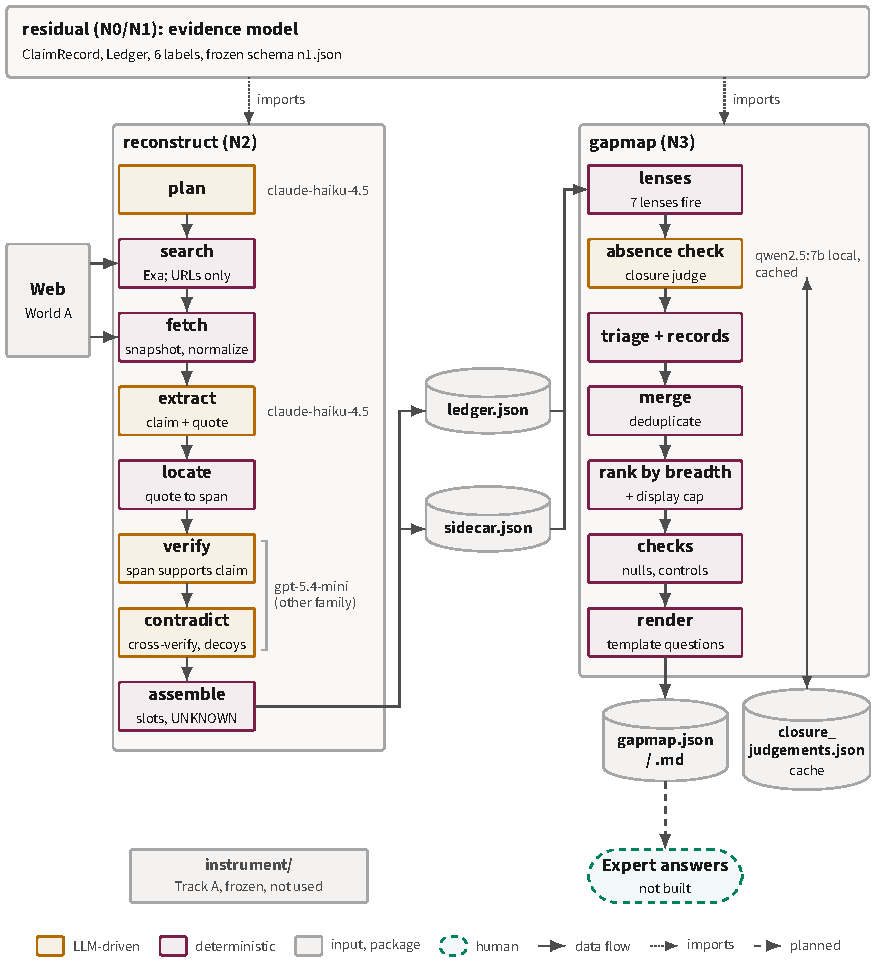
\includegraphics{figures/pdf/fig04_architecture.pdf}
  \caption[Implemented PoC architecture]{The implemented PoC: three packages, one direction of
  dependency, the artifacts written between them, and the external models each stage calls. Solid
  boxes and arrows exist in code and are offline-tested; most have also completed on a live run,
  but cross-verify and the current decoy stage have not completed live without a defect
  intervening (\cref{sec:not-demonstrated}). The human step at the far right does not exist yet in
  the PoC.}
  \label{fig:architecture}
\end{figure}

\begin{table}[tbp]
  \centering
  \small
  \caption{The three NOW packages: purpose, size, and tests. Test counts are from running each
  suite live on 2026-09-29 (\code{uv run --directory <pkg> pytest -q}), not from a grep-based
  count of test functions in the source.}
  \label{tab:packages}
  \begin{tabularx}{\linewidth}{@{}lp{3.1cm}rrX@{}}
    \toprule
    Package & Purpose & LOC & Tests (run) & Runtime dependencies \\
    \midrule
    \repo{residual/} & Typed evidence model: claim record, six epistemic labels, gates &
      1{,}281 & 268 & stdlib + \code{pydantic} only \\
    \repo{reconstruct/} & Populate a ledger from the open web, with verified provenance &
      4{,}803 & 416 & + \code{residual}; \code{httpx}, \code{openai}, \code{tldextract},
      \code{pypdf} \\
    \repo{gapmap/} & Read a ledger, propose ranked gap candidates and expert questions &
      2{,}986 & 172 & + \code{residual}; local Ollama over \code{urllib} \\
    \bottomrule
  \end{tabularx}
\end{table}

\subsection{\code{residual/}: the evidence model (N0/N1)}

\repo{residual/} defines the typed record of a claim, its provenance, and its epistemic label; it
is the domain-neutral core that N2 and N3 both write to and read from. \evobs{} It depends at
runtime only on \code{pydantic}, checked by the test
\code{test_modules_import_only_stdlib_pydantic_and_residual}. Nine modules (counting \code{__init__.py}, as for the other two packages) total 1{,}281 lines,
covering the claim record, its provenance types, the ledger, the evidential gate, the N1 feature
definitions, and the freeze mechanism. The module-by-module inventory is in \cref{app:reproduce};
the claim record, labels, and provenance chain are detailed in \cref{sec:evidence-model}.

\subsection{\code{reconstruct/}: the reconstruction pipeline (N2)}

\repo{reconstruct/} populates an N1 ledger for one \code{(domain, task)} pair from the open web,
with real provenance. Ten modules, 4{,}803 lines, 416 tests, none of which calls a live model or
the network (fakes only); a live run needs \code{python -m reconstruct.run --live} with a hard
\code{--max-usd}. The pipeline (\repo{reconstruct/src/reconstruct/run.py},
\repo{reconstruct/src/reconstruct/evidence.py}) is one \code{reconstruct(domain, task, ...)} call,
strictly one-way, with no agent loop:

\begin{enumerate}[noitemsep]
  \item \textbf{plan} -- propose 3--6 areas with search queries.
  \item \textbf{search / fetch} -- search via an OpenRouter web plugin; fetch, normalize, and hash
    each document once into a content-addressed snapshot store.
  \item \textbf{extract} -- one model call per document, pulling schema-bound candidate assertions.
  \item \textbf{locate} -- the extractor's quote must occur verbatim, after normalization, in the
    document's own normalized text, or the extraction produces no \code{Evidence} at all.
  \item \textbf{independence} -- union-find over fetched documents. Two documents merge into one
    cluster when their registrable domain matches (a hand-listed set of multi-organization
    domains, e.g.\ \code{arxiv.org}, is grouped by full host instead), or when their 5-shingle
    overlap is at least 0.5. Corroboration is counted per independent cluster.
  \item \textbf{verify} -- a second model, from a different model family than the extractor's,
    judges support on an annotated window around the located span.
  \item \textbf{cross-verify} -- claims sharing an area are cross-checked against topically-near
    claims from a different independence cluster; a contradicting verdict becomes a
    \code{Contradiction} record.
  \item \textbf{slot status and decoys} -- each (area, probe) pair is marked covered, thin,
    unknown, unverified, or unexamined. A \code{ClaimRecord} with no evidence enters the ledger
    only under \code{unknown}: searched, fetched, and fully verified, with nothing found. Decoy
    mutations (number, negation, scope) estimate a false-accept rate for the verifier.
\end{enumerate}

\repo{reconstruct/models.json} configures planner, extractor, and baseline as
\code{anthropic/claude-haiku-4.5} (family anthropic) and the verifier as \code{openai/gpt-5.4-mini}
(family openai), all served through one OpenRouter backend. The verifier's family must differ from
the extractor's, checked in code, so no claim can move off \emph{pending}/\emph{synthetic} on a
self-verification.

A real completed run (\repo{reconstruct/runs/20260928T133336Z-59ec876b3d7e/}, domain
\enquote{industrial machine maintenance}, task \enquote{PLC intermittent-fault diagnosis}) produced
375 claims: \code{literature_supported} 321, \code{synthetic_extrapolation} 49,
\code{unknown} 5. It drew on 35 fetched sources across 27 independent clusters, for a total cost of
\$0.679 across 473 logged model and search calls. \evobs{} This run left no claim pending. But
neither cross-verify nor the current decoy stage has completed on any live run without a defect
getting in the way. The one run that exercised both, GDPR v2
(\repo{reconstruct/runs/20260928T145943Z-bc1cc9a30a02/}), hit a provider-error defect (since fixed,
\cref{app:defects} row EL10) that left 140 of 366 evidence items pending. That is why 305 of its
523 claims read \code{synthetic\_extrapolation}. That run is not N3-admissible on its own
(\cref{app:claims}, row E23).

\subsection{\code{gapmap/}: the methodology-guided gap map (N3)}

\repo{gapmap/} reads one N2 ledger and proposes gap \emph{candidates}: it never writes a
hypothesis back into a ledger as a claim, and its scores never feed a gate as a criterion. Twelve
modules, 2{,}986 lines, 172 tests, all offline against a fake judge; the CLI replays a committed
judge cache by default. Seven methodology lenses (\code{lenses.py}) fire over criterion-labeled
claims only, each looking for a different missing element:
\begin{itemize}[noitemsep]
  \item \textbf{DISC} -- a judged term attached to multiple claims, no discriminating case;
  \item \textbf{DIAG} -- rival causes with no distinguishing sign;
  \item \textbf{SEL} -- a selection rule with no stated criterion;
  \item \textbf{HEDGE} -- a hedged rule with no exception stated;
  \item \textbf{GUARD} -- an error-avoidance step with no named check;
  \item \textbf{WHY} -- a procedure with no stated rationale;
  \item \textbf{RESULT} -- a test with no stated interpretation.
\end{itemize}
A fired candidate is judged for closure by \code{semantic.judge_candidate} against retrieved
sentences from the same ledger. It is then assembled into a three-tier \code{Record}
(\code{observed_evidence}, \code{inferred_gap}, \code{hypothesis}) and ranked by breadth, not by a
confidence calibrated against any gold (\cref{sec:evidence-model,sec:n3}).

\evobs{} The closure judge is \code{qwen2.5:7b-instruct}, served by a \textbf{local Ollama} instance at
zero cost, chosen because its model family (local) differs from both the ledger's extractor
(anthropic) and verifier (openai) families. This is a decision 0008 requirement, checked by code
review rather than by a test. Judgments are cached to \code{research/n3/<run>/closure_judgements.json},
keyed by \code{sha256(model_id, prompt)}. The CLI's default mode raises an error naming
\code{--judge ollama} on a cache miss, instead of silently calling the network, so a default run
and the test suite both touch no network at all.

\subsection{Determinism, replay, and budget}

Each package's reproducibility guarantee matches what it can and cannot control. \evobs{}
\repo{residual/} is pure, deterministic \code{pydantic} validation with no model or network call.
\repo{reconstruct/} is not deterministic end to end --- it makes live web and live model calls. But
every criterion-labeled claim traces to a byte-fixed snapshot span (\cref{sec:evidence-model}), and
every call is logged, even on failure. \repo{gapmap/} is fully offline by default: its one
model call is cached and replayed by content hash, so a default run and \code{pytest} touch no
network; only \code{--judge ollama} adds new cache entries.

A budget check accumulates cost \emph{before} each call and raises before overspending, writing the
three output files with \code{complete=False} rather than truncating silently. This is a real
constraint, not a theoretical one: N2's post-fix live re-check (E-LIVE v3) never got past its
first call. It was blocked by an exhausted \$5/week OpenRouter key, a provider-side limit
(HTTP 403), not by the code's own check firing. Failed calls are counted per task, making a loss
visible in \code{sidecar.json}. The \code{complete} flag itself, though, is computed independently
of that count, so a run can still read \code{complete=True} after calls have failed. The E-LIVE v2
defect (\cref{app:defects}, row EL10) was exactly this gap. \code{gapmap} narrows the equivalent
risk on its own side: a malformed or out-of-range judge answer is routed to its own retrieval-gap
category, \code{RG-UNDECIDED}, never silently treated as \enquote{open}. This was the fix for a
defect found by adversarial review (\cref{app:defects}, row L7). Module inventories and the budget
and freeze mechanisms' exact fields are in \cref{app:reproduce}.

\section{The evidence model}
\label{sec:evidence-model}

\subsection{The claim record}

The atomic unit of the whole PoC is the \code{ClaimRecord}
(\repo{residual/src/residual/claims.py}), a frozen \code{pydantic} model with fields
\code{assertion}, \code{question}, \code{layer}, \code{knowledge_type}, \code{tacitness},
\code{scope}, \code{evidence}, \code{generation}, \code{derivation}, \code{searches}, and
\code{certainty}. \evobs{} A claim needs at least one of \code{evidence}, \code{searches}, a
\code{derivation}, or a model \code{generation} to exist at all. An assertion must be non-empty and
whitespace-normalized. \code{certainty} may only be set on a claim whose label is one of the three
that can act as a criterion (\cref{tab:labels}). Claims live inside a \code{Ledger}
(\repo{residual/src/residual/ledger.py}), which also holds \code{Contradiction} and \code{Area}
records and a \code{purpose} field restricted to \code{reconstruction}, \code{gold}, or
\code{surrogate}. A \code{gold} ledger holds only criterion-labeled claims. A \code{surrogate}
ledger holds only simulation output. The three never share a ledger, so held-out gold cannot be
contaminated by reconstruction or synthetic material. \Cref{fig:evidence} shows how a claim ties
back to the text that produced it.

\begin{figure}[tbp]
  \centering
  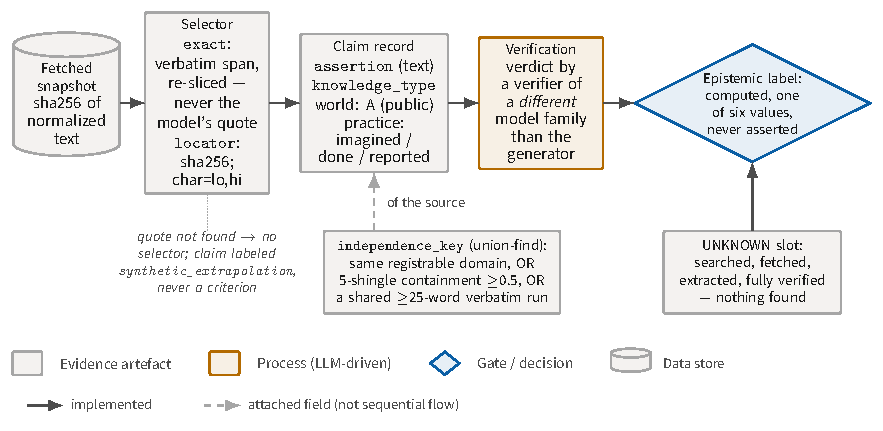
\includegraphics{figures/pdf/fig05_evidence.pdf}
  \caption[Provenance chain and label computation]{How a claim stays tied to its source: a
  fetched document is hashed once into a snapshot; a selector names an exact character span inside
  that hash; \code{ClaimRecord.label} is computed from the resulting evidence, never set by hand.}
  \label{fig:evidence}
\end{figure}

\subsection{Six epistemic labels, three of them criteria}

Every claim carries exactly one label, drawn from a closed enumeration
(\code{EpistemicLabel}, \repo{residual/src/residual/vocab.py}). \Cref{tab:labels} gives the exact
enum values and their plain-English meaning. \evobs{} Only three labels may ever act as a gate's
criterion (\code{CRITERION_LABELS}). A \code{Measurement} built by \code{gates.measure()} keeps
criterion labels apart from predictor labels. \code{evidential_gate} raises
\code{SyntheticRefused} on any \code{synthetic_extrapolation} input, and \code{GateRefusal} on
anything else outside \code{CRITERION_LABELS}, before the wrapped function runs at all. This is
the code form of the project's central rule: \textbf{synthetic output may be a predictor, never a
criterion}. A gap-map score, being derived from synthetic and inferred material, can rank
candidates for a human to look at; it can never decide a gate on its own.

\begin{table}[tbp]
  \centering
  \small
  \caption{The six epistemic labels (\code{residual.vocab.EpistemicLabel}), exact enum values.
  The first three are \code{CRITERION_LABELS}: the only labels an \code{evidential_gate} accepts.}
  \label{tab:labels}
  \begin{tabularx}{\linewidth}{@{}lXc@{}}
    \toprule
    Enum value & Plain-English meaning & May act as a criterion \\
    \midrule
    \code{observed_human_evidence} & Supported by a World C (human-record) source, or a
      human-record kind within World A & Yes \\
    \code{literature_supported} & Supported by a verified span in a public (World A) source & Yes \\
    \code{organisational_artefact_supported} & Supported by a verified span in an organization's
      own (World B) artifact & Yes \\
    \code{inferred} & No direct support, but derived from other claims via a \code{Derivation} & No \\
    \code{synthetic_extrapolation} & Produced or supported only by a model, with no verified
      human-authored span & No \\
    \code{unknown} & Searched for, fetched, and fully examined by another model family; nothing
      found & No \\
    \bottomrule
  \end{tabularx}
\end{table}

\subsection{The label as a computed property}

\code{ClaimRecord.label} is a Python \code{@property}, never a stored field: nothing in the code
base can set a claim's label directly. \evobs{} \repo{residual/src/residual/claims.py}
computes the label by a fixed rule, checked in this order. \emph{Supporting}
evidence means a SUPPORTS verdict after every exclusion reason --- self-verification, a
machine-voiced source, a software verifier, the wrong evidence world for the question --- returns
\code{None}:
\begin{enumerate}[noitemsep]
  \item simulated $\rightarrow$ \code{synthetic_extrapolation};
  \item supported by a World~C source, or a human-record-kind World~A source $\rightarrow$
    \code{observed_human_evidence};
  \item supported by a World~B source $\rightarrow$ \code{organisational_artefact_supported};
  \item supported by any other evidence $\rightarrow$ \code{literature_supported};
  \item an existing \code{Derivation} with no support $\rightarrow$ \code{inferred};
  \item a model \code{generation} with no support $\rightarrow$ \code{synthetic_extrapolation};
  \item otherwise $\rightarrow$ \code{unknown}.
\end{enumerate}
\code{Ledger.label} then
extends this for derived claims: an inference takes the \emph{weakest} of its premises' labels
(synthetic beats unknown beats inferred), so a chain of reasoning cannot bootstrap a strong label
from a weak one.

\subsection{Provenance chain}

Every fetched document is normalized exactly once (NFKC, quote/dash/bullet unification, whitespace
collapse) and hashed: \code{sha256:<text>}. \evobs{} A \code{Selector}'s \code{locator} names an
exact character span inside that hash, \code{sha256:<hash>;char=<start>,<end>}, and its
\code{exact} field is the literal slice of the normalized text -- never the model's own quotation.
A quote that cannot be located verbatim in the fetched text produces no \code{Evidence} at all. A
claim gains \code{Evidence} only through this re-slicing, which is why \code{verify_run.py} can
re-check every \emph{evidence item} in a run offline against its stored snapshot with no model
call. The chain is therefore: \textbf{snapshot hash} $\rightarrow$ \textbf{selector exact span,
re-sliced from the snapshot} $\rightarrow$ \textbf{claim}. Evidence from a quotable source kind is
required to carry an exact quote by a validator, not merely by convention.

\evobs{} This chain is independently checkable. \code{reconstruct.verify\_run} passes on all 909
evidence items across the three ledgers this report cites (PLC v1, GDPR v1, GDPR v2), re-slicing
every one against its stored snapshot with no model call. A separate, smaller sample was also
re-sliced by hand: 71 of 71 (\cref{app:claims}, row E25). Not every extraction reaches this chain.
When an extractor's proposed quote cannot be located, no \code{Evidence} is produced, and the claim
stays in the ledger with no supporting span. It is then labeled \code{synthetic\_extrapolation}:
418 of 1{,}169 claims across the three runs (49 PLC, 64 GDPR v1, 305 GDPR v2). For a slot that was
searched and fully verified with nothing found, the label is \code{unknown} instead: 34 more
(5, 14, 15). Together the two labels cover 452 of 1{,}169 claims (39\%) with no supporting span.
Such a claim is \textbf{not dropped}. Memorized model content can therefore enter the ledger, but
only under a label that cannot act as a gate's criterion (\cref{tab:labels}), so no lens or gate
reads it as a fact about the domain.

\subsection{Independence and contradictions}

Corroboration counts independent sources, not documents: \code{ClaimRecord.corroboration} is the
number of distinct \code{independence_key} values among a claim's supporting evidence. \evobs{}
Independence itself is computed by union-find over fetched documents
(\repo{reconstruct/src/reconstruct/evidence.py}, \code{independence_clusters}). Two documents
merge into one cluster when their registrable domain matches (a hand-listed set of
multi-organization domains, e.g.\ \code{arxiv.org}, is grouped by full host instead), or when
their 5-shingle containment is at least 0.5. A separate, span-level rule collapses syndicated
\emph{spans} of at least 25 verbatim words into one corroboration count without merging the
documents' clusters. This is a deliberate departure from an earlier whole-document rule that
over-merged unrelated documents (\cref{sec:n2}). Contradictions are a first-class \code{Ledger} record, not a
flattening step: when two claims from \emph{different} clusters, sharing an area, are cross-checked
and one verdict comes back REFUTES, that becomes a \code{Contradiction}.

\subsection{UNKNOWN is a searched-and-not-found result, never a blank}

A \code{ClaimRecord} with no evidence enters a reconstruction ledger under exactly one condition:
its (area, probe) slot was searched, fetched, extracted, and fully verified by another model
family, and nothing was found. \evobs{} Every weaker state -- \code{thin} (one supporting cluster,
not two), \code{unverified} (fetched but not fully verified), \code{unexamined} (nothing fetched) --
is tracked separately and never folded into \code{unknown}. This distinction matters because the
gap map's retrieval-gap category \code{RG-UNK} reads from exactly these \code{unknown}/\code{thin}/
\code{unverified} slots (plus ledger U-claims). A slot that was never searched is a retrieval
failure to fix, not an unstated fact about the domain.

\subsection{Evidence worlds and practice, as typed fields}

Three evidence worlds are a typed field on \code{Source}, not a narrative label:
\code{World.A = "public"}, \code{World.B = "organisational"}, \code{World.C = "human"}
(\repo{residual/src/residual/vocab.py}). \evobs{} A validator on \code{Source} requires a World~C
source to be a human-record kind, and requires exactly World~B sources to name their
\code{organisation}. A second typed field, \code{Practice}, distinguishes \code{imagined}
(prescribes work), \code{done} (records work), and \code{reported} (an account of work) -- the
Safety-II distinction between work-as-imagined and work-as-done. Both fields exist and are
enforced by the schema. \textbf{Only World A is populated in the PoC}: every N2 run to date
reconstructed from open-web text only, World~B has no ingestion adapter yet, and World~C has no
data at all.\footnote{Track A's instrument produces World~C-shaped records but is frozen outside
the NOW program (\cref{sec:scope}).}

\subsection{Residual accounting and the frozen schema, briefly}

\enquote{Residual accounting} names computing, per area, how much of a domain's claims carry each
epistemic label, and specifically how much of a target competence has no criterion-labeled support
at all. \evint{} \code{AreaFeatures} (per-area label, source-kind, tacitness, and contradiction
counts) and \code{ResidualAccount}/\code{EstimatedResidual} exist as types, and N2 computes the
features from real ledgers. But nothing yet computes an actual residual number against gold,
because no gold has been acquired. Decision 0006 hash-freezes the schema, the gap-map feature set,
and the label-deciding code together in \repo{residual/frozen/n1.json}. A \code{pytest}
architecture test fails if the live fingerprint diverges from the committed file, and changing any
of it needs a deliberate re-freeze and a commit explaining why. The exact fields, the three
SHA-256 hashes, and what each one covers are detailed in \cref{app:reproduce}.

\section{N0--N3: what was built and what it decided}
\label{sec:evolution}

Every NOW item is pre-registered to end in a continue, change, or stop reading of an experiment
result, never in \enquote{the build finished}. Rule R13 of the plan says so: a NOW item that ends in
infrastructure without a gate reading is a failure of the plan (\repo{REORIENTATION.md}, \S22).
\evobs{} N0 and N1 read their gates directly from a code check. N2's registered gate reads a specific
number against a specific floor. N3's registered gate, the ΔAUROC test against a gold standard, has
not run, because no gold has been acquired. What N3 reports below are its own internal
proof-of-concept checks, not its program gate. \Cref{tab:now-verdicts}
summarizes all four.

\begin{table}[tbp]
  \centering
  \small
  \caption{N0--N3: purpose, what was built, and the registered verdict each one read. Test counts
  and check results are the live-run numbers used throughout this report
  (\cref{sec:architecture,sec:n2,sec:n3}). N3's key commit, \code{ec45c31}, is the N3 PoC commit;
  \code{754e2e6}, cited elsewhere in this report, is the later ADR-0008 commit.}
  \label{tab:now-verdicts}
  \begin{tabularx}{\linewidth}{@{}lXXXl@{}}
    \toprule
    Item & Purpose & What was built & Registered verdict & Key commit \\
    \midrule
    N0 & Reset after the reorientation: fix the DOI-checking hook, freeze Track A, create the
      domain-neutral package & \repo{scripts/hook_tests/test_check_dois.py}; \repo{residual/}
      scaffold with its own test hook & \textbf{Done, gate passed} (2026-09-28): the hook
      demonstrably fires on a test edit & \code{d4fbc60} \\
    N1 & Pre-register and build the evidence model: claim record, six epistemic labels, gap-map
      field types, a freeze & \repo{residual/src/residual/} (claims, vocab, ledger, provenance,
      gates, gapmap, freeze, residual); \repo{residual/frozen/n1.json} & \textbf{Done, gate:
      continue with 2 additions} (\code{KnowledgeType.INTERPRETATION},
      \code{ResponseDistribution}), at the registered ≤2 limit & \code{accb506} \\
    N2 & Build a gated reconstruction pipeline and test it live and against planted falsehoods
      and private questions & One-way pipeline (plan→search→fetch→extract→locate→verify→
      contradict→assemble); E-LIVE runs on PLC and GDPR; E-PLANT/E-ABST harnesses & \textbf{Engineering
      PoC: complete. Full research validation: deferred.} Registered gate: \textbf{INCONCLUSIVE}
      -- E-PLANT's Continue branch closed on the validity floor ($a_U{=}5/24 < 8$), and the gated
      arms of E-PLANT and E-ABST were never scored & \code{ea5c18e} \\
    N3 & Build a methodology-guided gap map over N2's ledgers that turns silence into candidate
      hypotheses and expert questions & Seven lenses over three ledgers (PLC, GDPR v1, GDPR v2);
      ranked maps; built-in adversarial checks (anti-renaming, closure null, mismatched-evidence
      control, cross-run stability) & \textbf{PoC: pipeline complete, hidden-knowledge prediction
      not demonstrated.} Closure step is \code{closure-uninformative} on every lens tested. Program
      gate (ΔAUROC vs.\ gold) \textbf{not run} -- gold not acquired & \code{ec45c31} \\
    \bottomrule
  \end{tabularx}
\end{table}

N0 and N1 close cleanly: each reads a code-checked condition (a hook firing; a field-type count
against a pre-registered ceiling) and both pass. \evobs{} N2's registered research verdict is
INCONCLUSIVE. The ungated E-PLANT baseline adopted only 5 of 24 planted falsehoods
($a_U = 5/24$, below the required 8). By the pre-registered validity-floor rule, this closes the
\emph{Continue} branch before the gated arms of E-PLANT and E-ABST were scored, and those arms are
the actual test of whether gating helps. The owner then chose not to spend further budget. Those arms
and a post-fix live re-check (E-LIVE v3) stay pre-registered and unexecuted. Separately, N2's
engineering milestone is complete (\cref{sec:architecture}).

N3 built and ran its full pipeline on real ledgers. Its mismatched-evidence-control check is built into
\code{gapmap/checks.py}, added after an adversarial review found the weakness, and re-run on every
replay. It shows that the closure judge does not beat the mismatched-evidence control on any lens
tested (lenses with fewer than two candidates are skipped). The own rate equals the control rate
($0.889/0.889$, $0.961/0.961$, $0.958/0.958$). The gap map is therefore a
working mechanism that produces \emph{candidates}, with no demonstrated ability yet to tell a real
absence from a topically nearest neighbor's evidence.

\subsection{The owner exception: N3 on N2's engineering milestone}\label{sec:owner-exception}

N2's own registered gate stayed INCONCLUSIVE. Under the plan's rule R13, that would block the next
item from starting. \evobs{} The owner made a single, recorded exception (\repo{REORIENTATION.md},
\S22; \repo{PROGRESS.md}). N2's engineering milestone was treated as sufficient to start N3; N2's
research validation stays deferred. N3's own stop rule is unaffected, since it reads N3's own
ΔAUROC test, not N2's gate.

\evint{} This was a softened gate, and the person who softened it is the person whose program depends
on it. No one outside the project read the gate or approved the exception. Recording the exception is
better than leaving it implicit, but it is not independent control. The program therefore adds an
external gate reader: an independent statistician, or a small advisory board with one, reads the
closure, screening and H2 gates (MS1, MS3, MS5) against the pre-registration and has authority over
them. Any later exception by the owner needs the reader's sign-off (\cref{sec:validation}).

\section{N2: reconstructing explicit knowledge from the open web}
\label{sec:n2}

N2 built and stress-tested the reconstruction pipeline, \repo{reconstruct/}, that turns a
\code{(domain, task)} pair into an N1 \code{Ledger} of claim records with verified provenance. This
section reports what running it live and against adversarial harnesses showed, including the
negative and inconclusive results. \evobs{} N2's registered research verdict is
\textbf{INCONCLUSIVE}: E-PLANT's Continue branch closed on the validity floor (the ungated model adopted
$a_U = 5$ of 24 planted falsehoods, below the required 8), and the gated arms of E-PLANT and E-ABST were never scored. Separately, the engineering milestone is
complete.\footnote{\repo{research/n2/closeout.md}.}

\Cref{sec:architecture} describes the pipeline stage by stage. Two facts about it matter for
reading the results. First, every evidence item carries an exact span re-sliced from the fetched
snapshot. Extractions whose quote cannot be located stay in the ledger, labeled
\code{synthetic_extrapolation}, and can never act as a criterion. Second, the cross-verify stage and
the current decoy stage are implemented and tested offline but have never run live. The v1 runs used
the older pairwise contradiction stage, and the one post-fix run (GDPR v2) logged no cross-verify or
decoy call.\footnote{\repo{reconstruct/runs/20260928T145943Z-bc1cc9a30a02/sidecar.json}:
\code{cross_checks} and \code{decoys} are empty.} N2 ran three experiments
(\cref{tab:n2-experiments}).

\begin{table}[tbp]
  \centering
  \small
  \caption{N2's three experiments. Only E-PLANT and E-ABST are pre-registered, gated experiments;
  E-LIVE is a sanity check with no gold and no threshold.}
  \label{tab:n2-experiments}
  \begin{tabularx}{\linewidth}{@{}lXX@{}}
    \toprule
    Experiment & Question & Criterion \\
    \midrule
    E-LIVE & Does the pipeline run on the live web without fabricating, mislabeling, or falling
      over? & Inspection of runs; no gold, no threshold \\
    E-PLANT & Does gating reduce adoption of a planted false value alongside real pages? & Exact
      one-sided McNemar test, gated vs.\ ungated, with a validity floor $a_U \geq \lceil n/3 \rceil$ \\
    E-ABST & On real but private questions, does the pipeline give fewer false answers than the
      raw model? & $\mathrm{FAR}_{\text{raw}} - \mathrm{FAR}_{\text{pipe}} \geq 0.20$, with
      $n_{\text{included}} \geq 20$ \\
    \bottomrule
  \end{tabularx}
\end{table}

\subsection{E-LIVE: two domains, three run versions}

\evobs{} E-LIVE ran the pipeline on two live domains with the same model configuration:
industrial PLC intermittent-fault diagnosis (technical, procedural) and GDPR data protection impact
assessments, DPIA (legal, normative). Three versions ran: v1 (pre-fix), v2 (post-fix; the PLC run
crashed), and v3 (blocked before any billed call). \Cref{tab:n2-elive} gives the per-run
numbers.\footnote{\repo{research/n2/e_live_report.md}, \S3 and \S5; recomputed from
\repo{reconstruct/runs/}\code{<run>/sidecar.json} and \code{ledger.json}.}

\begin{table}[tbp]
  \centering
  \small
  \caption{E-LIVE per-run counts. \enquote{Located} is the sidecar's \code{n_located}, one
  definition for all runs; the ledgers hold 337, 206 and 366 evidence items (GDPR v1 and v2 hold 206 and 366
  against an \code{n_located} of 204 and 351). \enquote{Unknown claims} is
  the ledger's \code{unknown}-label count, one per (area, probe) slot that was searched, fetched and
  fully verified with nothing found; it is a different quantity from N3's \code{RG-UNK} category
  (\cref{tab:n3-results}). GDPR v2 is defect-compromised: 140 of its 366 evidence items kept a
  \code{pending} verdict after silent verifier failures, so it is not N3-admissible. PLC v2 crashed on
  a PDF encoding defect (0 claims, not shown).}
  \label{tab:n2-elive}
  \begin{tabularx}{\linewidth}{@{}lrrrrrr@{}}
    \toprule
    Run & Sources & Extracted & Located & Verified (supports) & Unknown claims & Cost \\
    \midrule
    PLC v1 & 35 & 370 & 337 & 321 & 5 & \$0.679 \\
    GDPR v1 & 20 & 259 & 204 & 195 & 14 & \$0.500 \\
    GDPR v2 & 25 & 523 & 351 & 207 & 15 & \$1.002 \\
    \bottomrule
  \end{tabularx}
\end{table}

GDPR v1's 14 of 35 (area $\times$ probe) UNKNOWN slots concentrate in \code{failure_mode} (5 of 5
areas): regulator and statute text states obligations, not how a DPIA goes wrong in practice.
\evint{} This is consistent with the kind of gap the gap map is built to flag, but it is not
validated against any ground truth.

\textbf{Exact spans.} \evobs{} The full check \code{reconstruct.verify_run} re-slices all 909
evidence items of the three completed runs exactly from their local snapshots (337 + 206 + 366). A
closeout sample by one AI inspector re-sliced 71 of 71.\footnote{\repo{research/n2/e_live_claim_inspection.md};
\repo{research/n2/e_live_report.md} \S6.2. The inspector was an AI agent, not a human. The snapshots
are git-ignored, so \code{verify_run} cannot be repeated from a fresh clone.} The claims are a
different matter. Of 1,169 claims in the three ledgers, 418 are labeled
\code{synthetic_extrapolation} (49, 64 and 305) and 34 \code{unknown}, so 452 have no supporting
span.\footnote{Labels computed with \code{ClaimRecord.label} over the three \code{ledger.json}
files.} Model-written and memorized content can therefore enter the ledger, but only under a label
that no lens and no gate reads.

\textbf{Cross-family verification.} \evobs{} A supporting verdict comes from a model of a different
family than the extractor (\code{openai/gpt-5.4-mini} vs.\ \code{anthropic/claude-haiku-4.5}), and a
same-family verdict cannot yield a criterion label. On sampled natural claims the verifier's main
error is scope drift, not fabrication: 30\% error on PLC v1 in the closeout inspection (Wilson 95\%
CI 15--52\%, $n=20$; the earlier v1 review estimated about 20\% drift), and 12\% on the current
verifier's GDPR v2 sample (Wilson 4--30\%, $n=25$, in-sample against prompts that quote these review
examples). Every GDPR drift case has one shape: a national list item is generalized to \enquote{a
DPIA is required} with the jurisdiction dropped.

\textbf{Decoy false accepts.} \evobs{} The v1 runs also tested the verifier with decoys: 20
supported claims per run, each mutated by negation, a changed number or a changed scope, and checked
again against the original span. The verifier accepted 7 of 20 decoys on PLC v1 (35\%, Wilson 95\% CI
18--57\%) and 3 of 20 on GDPR v1 (15\%, 5--36\%).\footnote{\repo{reconstruct/runs/20260928T133336Z-59ec876b3d7e/sidecar.json}
and \repo{reconstruct/runs/20260928T135354Z-eb840a85b7d1/sidecar.json}, key \code{decoys};
\repo{research/n2/e_live_review_notes.md} \S10.} On PLC, all 5 scope decoys were accepted, with 1 of
13 negations and 1 of 2 number changes. The measurement is weak in both directions. A review found
that 3 of the 5 PLC scope decoys only drop a conjunct, so the span still entails them; without those
three, the rate is 4 of 17 (24\%, 10--47\%). The decoy verifier also saw the exact span without the
surrounding context real verification gets, and the decoy stage was changed afterwards and has never
run live. The GDPR decoys were valid and exposed a real weakness: the verifier accepted
\enquote{or} changed to \enquote{and}. \evint{} What this means: the label
\code{literature_supported}, which every lens reads, rests on a verifier that accepted between a
quarter and a third of mutated PLC claims in the only measured run. Lens firings built on such claims
inherit that error; a false \enquote{supported} claim can seed a gap candidate.

\textbf{Defects found live.} \evobs{} Running on the real web, not the offline suite, surfaced
eleven defects that 416 passing offline tests had missed. They were error pages counted as sources,
rejected PDFs, dead corroboration, over-merged independence clusters, verifier scope drift, a false
contradiction, a lenient coverage rule, repeated failed fetches, a mislabeled report, verifier
failures hidden behind \code{complete: true}, and a PDF encoding crash. \Cref{app:defects} lists
each with its mechanism and fix commit; none of the fixes was re-checked live.

\subsection{E-PLANT and E-ABST: what they test, and why the verdict is inconclusive}

Both experiments compare a \emph{gated} pipeline arm (reconstruction plus verification) with an
\emph{ungated} raw-model baseline. Both were pre-registered with a stop rule fixed before any data
was seen.\footnote{\repo{docs/n2-eplant-eabst-protocol.md}, registered \code{3b72fb8}, with
amendments 1--2.} Both ran on two domains other than PLC and GDPR: home food safety (cooling and
reheating leftovers) and cold-weather concreting.

\textbf{E-PLANT}, in plain words: give the raw model a false planted value alongside real pages
that state the truth, and see whether it repeats the false value. The registered expectation, that
the ungated model would adopt the plant on more than 60\% of targets, was taken from ClashEval
\parencite{wu2024clasheval}. That figure holds only for GPT-4o (61\%) and GPT-3.5 (63\%), on questions
the model answered correctly without context, with the modified document as the only context; the
other four models adopted it 31--53\% of the time. In ClashEval's own test with four added
retrieved documents, context adoption fell. E-PLANT showed each plant among about 12 real pages per
domain that state the true value, a condition ClashEval did not test. The validity floor derived
from that figure was therefore miscalibrated.

\textbf{E-ABST}, in plain words: ask the raw model a real but private question it cannot look up,
and see how often it answers falsely instead of abstaining. Its response schema allows it to answer
\code{null}. \Cref{tab:n2-baselines} gives what was measured: the ungated baselines only.

\begin{table}[tbp]
  \centering
  \small
  \caption{E-PLANT and E-ABST ungated baselines (standing results; the gated arms were never
  scored). $a_U$ is the number of targets on which the ungated model adopted the planted value.}
  \label{tab:n2-baselines}
  \begin{tabularx}{\linewidth}{@{}lXrr@{}}
    \toprule
    Experiment & Result & $n$ & Wilson 95\% CI \\
    \midrule
    E-PLANT & $a_U = 5/24$ (21\%), below the registered validity floor $\lceil 24/3 \rceil = 8$ &
      24 & 9--40\% \\
    E-ABST & 5/24 private items answered, 19 abstained (79\%) & 24 & -- \\
    \bottomrule
  \end{tabularx}
\end{table}

\textbf{Why INCONCLUSIVE.} For E-PLANT, the validity floor $a_U \geq 8$ is not met ($a_U = 5$). By
the registered rule this closes the Continue route for E-PLANT, and therefore for N2, before any
gated arm is scored. It is a result about the sensitivity of the test, not about gating. The
baseline adopted too few plants for any gating benefit to be detectable. That may reflect the design
(plants among true pages) rather than model robustness. For E-ABST, only an answering
statement can be false, so $\mathrm{FAR}_{\text{raw}} \leq 5/n_{\text{included}}$, and the required
20-point margin is reachable only in a narrow corner (all five raw answers false, the pipeline giving
none).

\textbf{Gated arms: sealed, unscored.} \evobs{} E-PLANT's gated run~1 (tag \code{n2-freeze}) is
sealed and declared a defect-forced rerun unit, because failed calls were not logged at that tag;
run~2 never executed. E-ABST's pipeline run~1 is descriptive only (17 of 24 items produced zero
claims); run~2, second coding and unsealing never happened. \textbf{No statement about whether gating
reduces adoption of planted falsehoods, or false answers, is supported by this PoC.}

\textbf{Budget.} \evobs{} The post-fix live re-check (E-LIVE v3, both domains) never ran: both
attempts stopped at the planner's first call with \code{HTTP 403, "Key limit exceeded (weekly
limit)"}. This was the provider's key limit, not the pipeline's own \code{Budget} guard. N2's total
recorded spend was $\approx\!\$4.82$ against a \$5 weekly key limit: E-LIVE \$2.374, E-PLANT
\$1.953, E-ABST \$0.495. The three registered experiments' caps summed to about \$21.\footnote{\repo{research/n2/e_plant_eabst_report.md} \S3; \repo{research/n2/e_live_report.md}
sidecar costs, summed.} The owner chose not to raise the limit.

\begin{evobsbox}
\textbf{Registered verdict.} E-LIVE reads \emph{INCONCLUSIVE: the provenance core passes; the
post-fix pipeline was never checked live}. E-PLANT and E-ABST each read \textbf{INCONCLUSIVE}, and so
does N2: Continue needs E-PLANT to read Continue and the E-ABST margin to be met, and neither is
reachable from what ran. The floor failure closed Continue; the budget then stopped the gated arms
and the post-fix live check. Nothing in this report changes these readings; the
\emph{engineering-complete / research-deferred} split is the owner's addition to
them.\footnote{\repo{research/n2/closeout.md}; \repo{research/n2/e_plant_eabst_report.md} \S0;
\repo{research/n2/e_live_report.md} \S9.}
\end{evobsbox}

\begin{figure}[tbp]
  \centering
  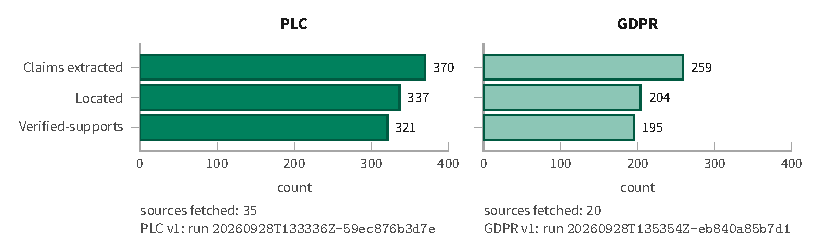
\includegraphics{figures/pdf/fig06_n2.pdf}
  \caption[N2 stage counts]{How much survives each N2 pipeline stage in the two v1 runs (PLC and
  GDPR): sources fetched, claims extracted, located (sidecar \code{n_located}), and verified as
  supported. GDPR loses more than twice the share PLC loses between extraction and location
  (21\% vs.\ 9\%); both lose about 5\% between location and support.}
  \label{fig:n2}
\end{figure}

\subsection{What N2 taught us}

\textbf{Plan the budget as part of the design.} \evint{} A key with a \$5 weekly limit met three
registered experiments whose caps summed to about \$21, and nobody checked headroom against the sum
of caps before running. N2 closed inconclusive partly for a budget reason: the floor failure closed
Continue, and the budget stopped the remaining arms. A pre-run headroom check is now a queued lesson.

\textbf{Silent failures can hide behind a \code{complete: true} flag.} \evobs{} In GDPR v2, 140
verify calls raised and left no trace, yet the sidecar reported \code{complete: true}; the same
provider event most likely cut off E-PLANT's sealed gated run~1. The fix logs every failed attempt
and counts skips per task. \evint{} The fix is partial: \code{complete} and the N3 input flag still
ignore \code{failed_calls_by_task}.

\textbf{Calibrate a \enquote{beats the baseline} gate before registering it.} \evint{} Both
experiments ran their ungated baseline before any gated arm, but nobody computed the reachable range
of the registered gate from it. E-PLANT's floor came from a condition (the plant as the only
context) that E-PLANT did not reproduce. E-ABST's \code{null}-offering schema set an abstention
ceiling the raw model met on its own, 79\% of the time. A future planted-falsehood design needs a
calibration pilot, printed as a \enquote{best reachable outcome}, before any gate is registered.

\section{N3: methodology-guided gap mapping}
\label{sec:n3}

N3 (\repo{gapmap/}) reads one N2 ledger and turns silences in it into inspectable candidates: a
place where the sources name a construct but do not state its content, with a hypothesis about what
a practitioner would add. \Cref{sec:architecture} describes the package's modules. This section
reports what the pipeline produced on three real N2 ledgers, and the checks that expose its central
weakness.

\evobs{} N3's registered status is \textbf{PoC pipeline complete; hidden-knowledge prediction not
demonstrated.}\footnote{\repo{research/n3/README.md}.} The registered gate that would test prediction (E-CTA,
E-OSS against held-out gold; restructured as V2 and H-OSS in \cref{sec:validation}) has not run: no gold has been acquired, and the absence check does not
beat its fair control (\cref{sec:absence-check}).

\textbf{What the lenses read.} \evobs{} Lens firing rules, the stem index, every anchor and the
judge's seed text all run on the extractor's paraphrase of a claim (its \code{assertion}), not on the
verbatim span. The knowledge types that gate DIAG, GUARD and HEDGE were also assigned by the
extractor. Spans are kept for display and for the quotes in questions.\footnote{\repo{gapmap/src/gapmap/lenses.py}
(\code{_diag_anchor}, \code{_best_sentence}); \repo{gapmap/src/gapmap/link.py};
\repo{gapmap/src/gapmap/semantic.py}.} The PoC's gap candidates are therefore built on model-written
text that is tied to, but not identical with, the source.

\subsection{The seven lenses}

Each lens names a construct drawn from the methods review (\cref{sec:foundations}) and fires when the
ledger attests that construct without stating its content. \Cref{tab:n3-lenses} summarizes them;
\cref{app:lenses} gives each firing rule and human channel.

\begin{table}[tbp]
  \centering
  \small
  \caption{The seven methodology lenses. Firing rules and elicitation channels are in
  \cref{app:lenses}.}
  \label{tab:n3-lenses}
  \begin{tabularx}{\linewidth}{@{}lXX@{}}
    \toprule
    Lens & Missing element & Predicted knowledge type \\
    \midrule
    DISC & Boundary of a judgment term & cue, perceptual or collective \\
    DIAG & A sign that tells rival causes apart & interpretation, cue \\
    SEL & Situation $\rightarrow$ option mapping & decision \\
    HEDGE & The exception condition on a hedged rule & decision \\
    GUARD & How an automated error is noticed & check, automated \\
    WHY & The rationale for a prescribed step & rationale \\
    RESULT & What a test result means and where it leads & interpretation, expectancy \\
    \bottomrule
  \end{tabularx}
\end{table}

A lens fires over criterion-labeled claims only (never over \code{synthetic_extrapolation} or
\code{unknown} claims). Each firing becomes a \emph{candidate}, not yet a gap. \evobs{} Lens firing
tracks each domain's texture, as designed: DIAG fires only on PLC, the diagnostic domain, while DISC
and HEDGE fire mainly on GDPR, the normative domain (\cref{tab:n3-firing}). This shows that the lenses
distinguish domain texture, not that they find hidden knowledge.

\begin{table}[tbp]
  \centering
  \small
  \caption{Lens firing per ledger, recomputed offline with \code{gapmap.lenses.run_all}.
  \enquote{Promotional seeds excluded} counts candidates dropped before judgment by the domain
  denylist.}
  \label{tab:n3-firing}
  \begin{tabularx}{\linewidth}{@{}lrXr@{}}
    \toprule
    Ledger & Candidates fired & By lens & Promotional seeds excluded \\
    \midrule
    PLC & 56 & WHY 24, RESULT 19, DIAG 9, SEL 2, DISC 1, GUARD 1 & 42 \\
    GDPR v1 & 51 & RESULT 21, DISC 13, WHY 8, HEDGE 5, SEL 4 & 8 \\
    GDPR v2 & 48 & DISC 14, SEL 11, RESULT 9, WHY 9, HEDGE 5 & 1 \\
    \bottomrule
  \end{tabularx}
\end{table}

\subsection{The absence check: closure}
\label{sec:absence-check}

Firing a lens only shows that a construct is named. Deciding that its content is really
\emph{unsaid} (\code{closure} in code) needs a second step. The PoC tried two versions.

\textbf{Lexical closure (first version).} A stem co-occurrence rule scored a candidate closed if
another claim shared enough stems with the missing element. \evobs{} Against a donor-claim null
(200 random-donor draws, self and same-source claims excluded from both arms), the final maps'
observed lexical-closure counts fall within or below the null's 5--95\% interval on every ledger (PLC
below it): PLC 22 against a null mean of 33.48 (26--41), GDPR v1 11 against 12.735 (8--17), GDPR v2
11 against 8.08 (5--12).\footnote{\repo{research/n3/plc/gapmap.json},
\repo{research/n3/gdpr_v1/gapmap.json}, \repo{research/n3/gdpr_v2/gapmap.json}, field
\code{checks.lexical_donor_null}; \code{CLOSURE_NULL_DRAWS} in \repo{gapmap/src/gapmap/config.py}.
Pre-final maps reported other figures; they are historical.} Lexical closure did no better than
chance.

\textbf{Semantic closure (final version).} A local judge (\code{qwen2.5:7b-instruct} over Ollama,
temperature 0, cached and replayable) reads the sentences a lexical retriever pulls from the ledger,
up to 8 verified and 4 unverified per probe, and decides whether the missing element is stated:
\code{closed}, \code{partial} or \code{open}. DIAG probes each rival cause separately, so a DIAG
record can rest on more sentences (34 and 50 in the two PLC DIAG records).

\evobs{} The map's fair control keeps the seed's own sentences in both arms and swaps only the
other-source sentences for those of the topically nearest candidate of the same lens. Lenses with
fewer than two candidates are skipped. The judge's closure rate, counting \code{partial} as closed,
is the same in both arms: \textbf{PLC 0.889, GDPR v1 0.961, GDPR v2 0.958} ($n = 54, 51, 48$).
Every tested lens in every ledger is flagged \code{closure-uninformative}
(\cref{fig:closure}).\footnote{\repo{research/n3/}\,(\code{gapmap.json} in each domain folder), field
\code{checks.mismatched_evidence_control}.}

Four qualifications keep this result in proportion.\footnote{The paired figures come from an
offline replay of the committed judge caches with the package's own functions, made for the review of
this report; they are not yet an output of \repo{gapmap/src/gapmap/checks.py}.} First, in 32 of the
153 pairs (PLC 8, GDPR v1 11, GDPR v2 13) the two arms sent the judge an identical prompt, so equality
there holds by construction. Second, the rate counts \code{partial} as closed, while triage keeps
partial candidates; counted on \code{closed} alone, own versus control is 0.30/0.33, 0.65/0.61 and
0.58/0.52, still far below the 0.20 difference the check requires. Third, the own rate is 1.0 on 11
of the 14 tested lens--ledger cells, so the test has little room to separate the arms. Fourth, an arm
with the seed's and same-source sentences removed still closes or partly closes 0.667, 0.725 and
0.708 of candidates, which fits a lenient judge as well as any other mechanism.

\evint{} The reading is narrow: the judge's verdict does not depend on which evidence it is shown,
so it is not yet an informative absence check. Every candidate should be read as \enquote{a lens
fired here}, not as \enquote{experts know something here}.

\evobs{} How this was found matters. An adversarial AI review of the pre-final maps found that the
absence check did not beat a fair control; the first built-in control had been a straw man that
\enquote{passed}. The fair control was then written into \repo{gapmap/src/gapmap/checks.py}, raised
the \code{closure-uninformative} flag on the final maps, and is re-run on every replay.

\begin{figure}[tbp]
  \centering
  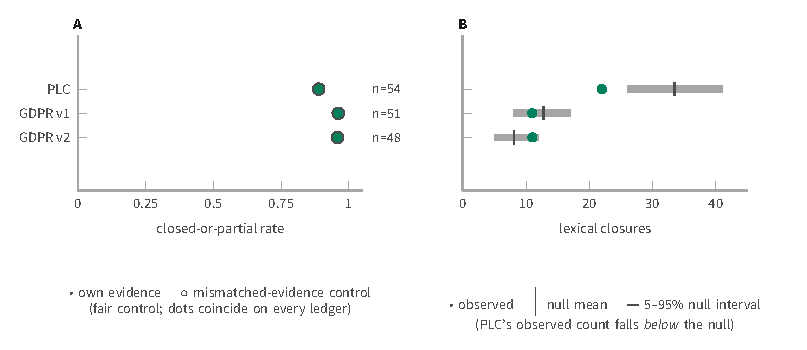
\includegraphics{figures/pdf/fig08_closure.pdf}
  \caption[The absence check versus its fair control]{Panel A: closed-or-partial rate of the
  closure judge on a candidate's own evidence and on the fair control (other-source sentences swapped
  for the topically nearest candidate's), by ledger. The rates are equal in every ledger: the judge's
  verdict does not depend on which candidate's other-source evidence it is shown. Panel B: observed
  lexical closures against the donor null (mean and 5--95\% interval of 200 draws).}
  \label{fig:closure}
\end{figure}

\subsection{Triage: retrieval gaps versus gap candidates}

A candidate that is not closed is sorted into one of two kinds (\cref{sec:evidence-model} gives the
taxonomy):

\begin{itemize}[noitemsep]
  \item \textbf{Retrieval gaps}: thin support, not a hidden-knowledge signal. \code{RG-UNK}
    (nothing found for a searched, fully examined slot), \code{RG-SINGLE} (only one independent
    source discusses the topic), \code{RG-UNVER} (closed only by an unverified or synthetic
    sentence), \code{RG-SIBLING} (the same anchor closes in an independent sibling reconstruction)
    and \code{RG-UNDECIDED} (the judge's answer could not be parsed; never defaulted to
    \code{open}). Their action is to search or verify further, not to ask a human. One GDPR v2
    \code{RG-SIBLING} record still carries a hypothesis and a question, because the sibling step
    changes the category without clearing them; this is a defect (\cref{app:defects}).
  \item \textbf{Gap candidates} (category \code{HYP}): a three-tier record of
    \code{observed_evidence} (the verbatim spans, each with its label and verdict),
    \code{inferred_gap} (the closure judgment and its reasoning, re-runnable from the cache) and
    \code{hypothesis}, a hidden-knowledge hypothesis whose label is fixed to \code{inferred}. A record
    is HYP when its state is \code{open} or \code{partial}, at least two independent sources
    discuss the topic, and no retrieval-gap rule applies first.
\end{itemize}

\subsection{Ranking, display cap and template questions}

Candidates are ranked by \textbf{breadth}, a rubric (\code{confidence_rubric} in
\repo{gapmap/src/gapmap/record.py}): score $= A + B - P - Q$, where $A$ buckets the number of
independent sources that discuss the topic, $B$ rewards step breadth, and $P$ and $Q$ penalize a
\code{partial} state and a promotional seed. It is \emph{not} expected information gain (EIG); EIG-based
selection is future work (N6). A single-source candidate becomes \code{RG-SINGLE}, never a
hypothesis.

\evobs{} After merging near-duplicate records, the map applies a display cap: at most 12 records, 3
per lens and 4 per area (\code{MAP_TOP_N}, \code{MAP_PER_LENS}, \code{MAP_PER_AREA} in
\repo{gapmap/src/gapmap/config.py}). Records beyond the cap are dropped from the output; they are
not moved to the retrieval gaps. On PLC this removes 15 of 24 merged HYP records (10 RESULT, 5 WHY);
the GDPR maps are not affected.\footnote{Offline replay of \code{rank.merge} and \code{rank.build}
from the committed judge cache.} The cap is per lens, so it also shapes the lens mix of the displayed
map. Any future area score must be computed over the uncapped set.

Each expert-facing question is \textbf{filled from a Python f-string template, not by a model
call}: a fixed interview frame (e.g., DISC: \enquote{Think of a recent case where you had to judge
whether something was \{anchor\}\ldots}) with up to two quotes from distinct independence keys. A
quote is the most relevant verbatim span sentence; when no usable sentence exists, the code falls
back to the extractor's assertion and still sets it in quotation marks (GDPR v1's only candidate is
such a case, \cref{app:records}).

\subsection{Built-in checks}

Every map carries its own checks, so a reader does not have to trust an unaudited ranking:
anti-renaming (does the ranking reproduce evidence density? Jaccard overlap with density-sorted
rankings and a Spearman correlation), the fair mismatched-evidence control and the lexical donor
null (\cref{sec:absence-check}), and cross-run stability across the two independent GDPR
reconstructions. The committed maps replay byte-identically from the committed judge caches with no
network call (\cref{app:reproduce}).

\subsection{Results per domain}

\Cref{tab:n3-results} gives the final map counts. Map lengths in the committed JSON (10, 2 and 7)
each include one \code{CONTROL} slot, which targets the area with the highest attested share that
produced no hypothesis, on top of the HYP records.

\begin{table}[tbp]
  \centering
  \small
  \caption{N3 final maps, per domain. GDPR v2 is not N3-admissible (140 of 366 evidence items kept a
  \code{pending} verdict, \cref{sec:n2}) and is shown only for the cross-run check. RG-UNK is the N3
  retrieval-gap category (it recombines unknown, thin and unverified slots at the claim level), a
  different count from N2's unknown claims in \cref{tab:n2-elive}.}
  \label{tab:n3-results}
  \begin{tabularx}{\linewidth}{@{}p{3.3cm}XXX@{}}
    \toprule
    & PLC & GDPR v1 & GDPR v2 (not admissible) \\
    \midrule
    HYP after merge (uncapped) & 24: RESULT 13, WHY 8, DIAG 2, GUARD 1 & 1: RESULT &
      6: RESULT 3, DISC 1, HEDGE 1, WHY 1 \\
    HYP shown after the display cap & 9: RESULT 3, WHY 3, DIAG 2, GUARD 1 & 1 & 6 \\
    Closure state of shown HYP & 3 open, 6 partial & 1 partial & 6 partial \\
    RG-SINGLE / RG-UNVER / RG-SIBLING / RG-UNK & 11 / 0 / n/a / 10 & 12 / 4 / 2 / 28 &
      3 / 6 / 7 / 44 \\
    \bottomrule
  \end{tabularx}
\end{table}

\evobs{} The three \code{open} records need a closer look. The two PLC DIAG records read
\code{open} although the judge marked 5 and 6 claims as partial: the DIAG rule counts a rival as
unsigned whenever its state is not \code{closed}, so a group of partially signed rivals reads
\code{open}. Only one of the 16 displayed candidates (PLC rank 7, a WHY record with three independent
sources) has no partial hit at all.\footnote{\repo{research/n3/plc/gapmap.json},
\code{map[*].inferred_gap.partial_hits}; the rule is in \code{semantic._judge_diag}.} For every
candidate, the lens fired; the absence check found the element at most partly stated.

\begin{figure}[tbp]
  \centering
  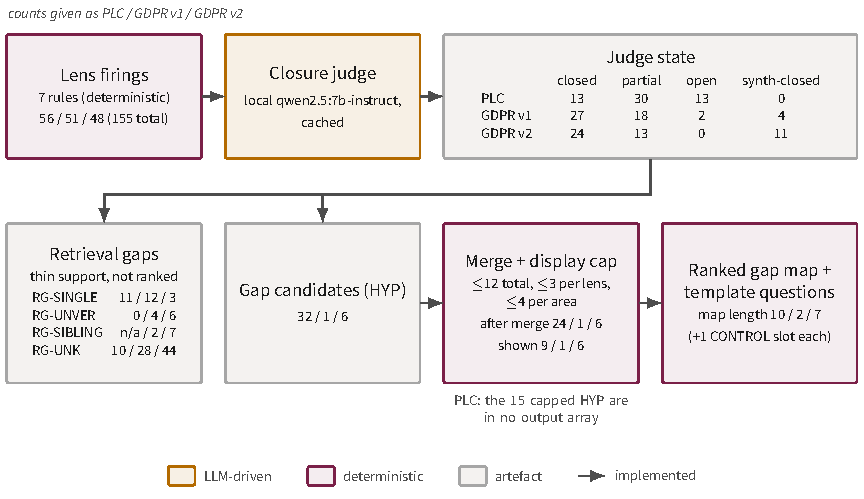
\includegraphics{figures/pdf/fig07_n3.pdf}
  \caption[From lens firing to gap candidate or nothing]{How lens firings become retrieval gaps, gap
  candidates or nothing, with counts per ledger (PLC / GDPR v1 / GDPR v2). After the closure judge
  and triage, near-duplicate HYP records are merged (PLC 24) and a display cap keeps at most 12
  records, 3 per lens and 4 per area (PLC 9 shown; GDPR unaffected). Most shown candidates are
  \code{partial}, not \code{open}.}
  \label{fig:n3}
\end{figure}

\subsection{The negative results, stated plainly}

\begin{itemize}[noitemsep]
  \item \textbf{The absence check ties its fair control on every ledger}, and lexical closure does
    no better than its donor null (\cref{sec:absence-check}).
  \item \textbf{13 of the 16 displayed gap candidates are \code{partial}}, and the two PLC DIAG
    records are \code{open} only by the DIAG rule. \evint{} The fair control counts \code{partial}
    as closed, so most surviving hypotheses sit in a state the map's own control would call
    \emph{closed}, an internal tension we state rather than hide.
  \item \textbf{Precision by adversarial judgment: 3 of 19 strict (8 of 19 lenient), on the
    pre-final maps only.} \evobs{} One adversarial AI reviewer (Opus) judged the pre-final maps'
    candidates, in-sample, with no human coder and no gold; the per-record tally is not committed.
    Wilson 95\% CIs, recomputed: 5.5--37.6\% and 23.1--63.7\%. The final maps were not re-tallied
    after two changes that altered the candidate set (the parse fix below and the fair-control
    rewrite). It is a reported sanity signal, never a measured precision of the committed maps.
  \item \textbf{PLC's ranking correlates with source density} (Spearman $\rho = 0.91$; overlap of
    the top ten with the ten highest-density candidates $J_{10} = 0.58$). \evint{} The anti-renaming
    check excludes \emph{low-density renamed} ($J_{10}$ with the lowest-density ten is 0.00), not
    \emph{high-density renamed}, so this direction is not what it was built to catch. On GDPR,
    $\rho$ is 0.09 and 0.16.\footnote{\repo{research/n3/plc/gapmap.json}, key
    \code{checks.anti_renaming}.}
  \item \textbf{Cross-run stability is low.} \evobs{} Of GDPR v1's 13 unclosed lens records (1 gap
    candidate, 12 single-source retrieval gaps), 3 have any counterpart in the independent v2
    reconstruction; of v2's 9 (6 gap candidates, 3 single-source retrieval gaps), 3 have a
    counterpart in v1. Every counterpart is partial. \evint{} The two runs are dominated by different
    independence keys, so the instability traces to retrieval, not to lens logic.
  \item \textbf{The judge-parsing defect was found by review, not by tests.} \evobs{} Unparsed
    judge answers silently defaulted to \code{open}, reported in \repo{docs/lessons.md} as 24 of 103,
    62 of 150 and 60 of 147 responses; the pre-fix caches are not committed, so these counts cannot
    be re-checked. The offline tests used a fake judge that always answered in the expected format.
    An unparsable answer now becomes \code{RG-UNDECIDED}.
\end{itemize}

\begin{findingbox}
N3's pipeline runs end to end and deterministically. Its central step does not work yet: the
absence check, which decides that a missing element is really unsaid rather than merely unquoted,
does not beat a fair, topically matched control on any tested lens in any of three ledgers. An
adversarial review found this weakness; the fair control now built into every map confirms it on
each replay. Everything downstream (hypotheses, ranking, questions) inherits it: the records are
\textbf{candidates} where a lens fired, not validated predictions of what an expert knows. The
falsifier ($\Delta$AUROC against held-out gold) has not run and should not run until closure passes a
human-labeled check. The correct reading is \emph{not demonstrated, and the current absence check is
not yet a valid instrument}, not that the human knowledge residual is unpredictable.
\end{findingbox}

\section{Demonstrations: complete traces from source to question}
\label{sec:demos}

The tables in \cref{sec:n2,sec:n3} report counts. This section follows one record end to end
(source, verbatim span, claim and label, lens, inferred gap, hypothesis and generated question) and
one record kept to show a known defect. Two further traces, one from each GDPR run, are in
\cref{app:records}. Quoted fields are copied from the committed \code{gapmap.json} files; where we
shorten, we say so. \textbf{Every record below is a candidate.} No expert has read or answered any of
these questions.

\evobs{} The traces were chosen by the author after the maps were final. The rule, stated after the
fact, is: the top-ranked record of each map, plus PLC's second record as a failure example. They are
not a random sample, and the top-ranked records are among the richest in the maps.

\subsection{Trace 1: PLC, rival causes of an intermittent fault}

PLC's top-ranked record merges six lens records into one DIAG group.\footnote{\repo{research/n3/plc/gapmap.json},
\code{map[0]}, \code{gap_id} \code{g-59164a9db5bd}; also \repo{research/n3/plc/gapmap.md},
\enquote{\#1 [DIAG]}.} \Cref{tab:trace1} gives the record and \cref{fig:trace} draws it.

\begin{table}[tbp]
  \centering
  \small
  \caption{Trace 1: PLC, lens DIAG, gap \code{g-59164a9db5bd}, category HYP, closure \code{open}.}
  \label{tab:trace1}
  \begin{tabularx}{\linewidth}{@{}p{2.4cm}X@{}}
    \toprule
    Stage & Content \\
    \midrule
    Seed source & \url{liambee.me/general/troubleshooting-plc-systems-a-systematic-approach-to-finding-faults} \\
    Seed span (verbatim) & \enquote{Loose terminals cause many intermittent faults. A flashlight
      reveals problems in dark panels that you miss otherwise.} \\
    Seed claim / label & \code{c-d7bce12d16755797}, \code{literature_supported}, verdict
      \code{supports}. The extractor's assertion, which the lens reads: \enquote{Loose terminal
      connections are a common cause of intermittent PLC faults and should be checked during
      troubleshooting.} The anchor is this assertion cut at 80 characters. \\
    Lens \& target & DIAG: 7 independent sources discuss the topic; the lens found 5 rival causes
      (ground loops, aliasing, installation vs.\ software, VFD/contactor noise, pull-up/clock
      timing) \\
    Inferred gap & Of 34 verified sentences retrieved, the judge found none that fully states a
      discriminating sign for any of the 5 rival causes; it marked 5 claims as partial (e.g.,
      \enquote{Sentences 1 and 4 partially address the distinction but do not explicitly state an
      observable sign}). DIAG treats a partially signed rival as unsigned, so the group reads
      \code{open}. \\
    Hypothesis (inferred) & \enquote{\ldots{} practitioners are predicted to tell these rival causes
      of \enquote{Loose terminal connections are a common cause of intermittent PLC faults and} apart
      by signs; the closure judge found a sign for the following (test DIAG:c-d7bce12d16755797):}
      followed by the five causes, each marked \enquote{(no sign found)} \\
    Question \& channel & \enquote{Sources list several causes of [anchor]: [two verbatim rival
      spans, from \url{automate.org} and \url{ecsintl.com}]. Think of the last time you diagnosed
      Loose terminal connections are a common cause of intermittent PLC faults and. Which cause did
      you suspect first, and what did you see, hear or measure that let you rule the others out?}
      -- CDM probes on a recalled case, then contrasting cases \\
    \bottomrule
  \end{tabularx}
\end{table}

\begin{figure}[tbp]
  \centering
  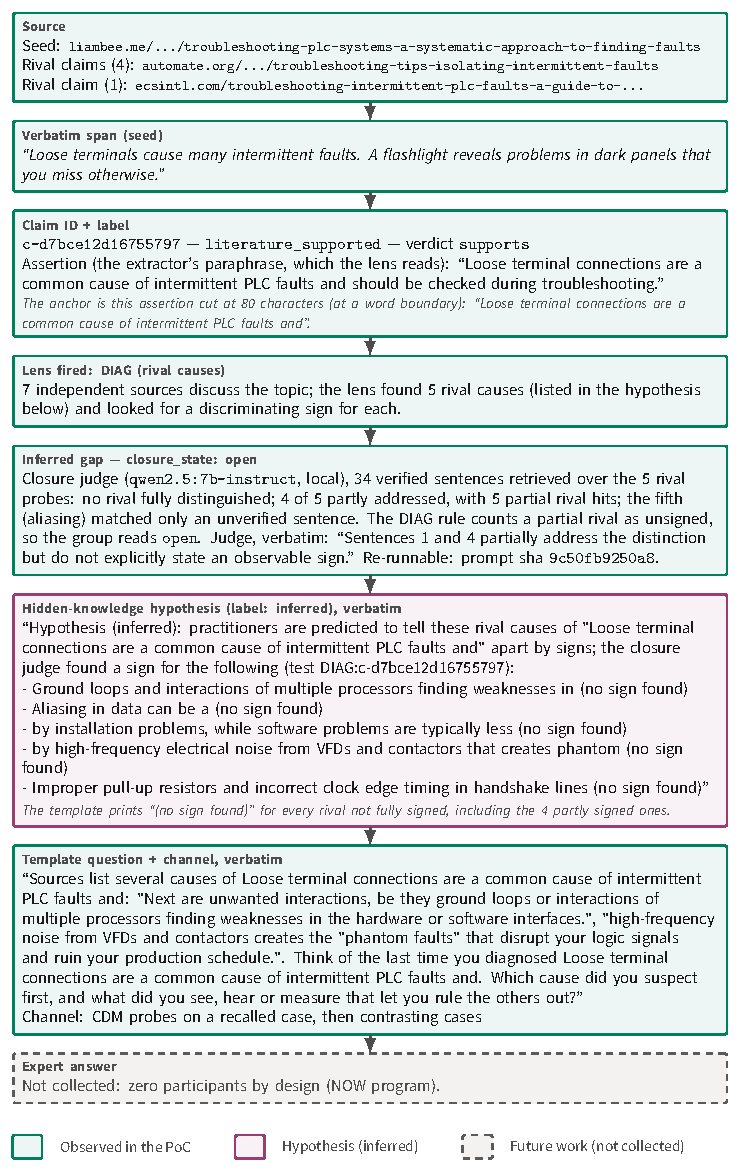
\includegraphics{figures/pdf/fig09_trace.pdf}
  \caption[One complete trace, source to question]{Trace 1, end to end: the seed span and its claim,
  the DIAG lens with five rival causes, the closure judge's verdict (no rival fully signed; 5 claims
  partly signed, which the DIAG rule counts as unsigned, so the record reads \code{open}), the
  hypothesis and the template question. The lens fired; the absence check found the element at most
  partly stated. No expert has answered the question.}
  \label{fig:trace}
\end{figure}

\textbf{Weaknesses.} The anchor is not a construct name but the extractor's assertion cut at 80
characters, so the question is not a grammatical sentence. The hypothesis template says the judge
\enquote{found a sign for the following} and then marks every item \enquote{(no sign found)}. The
\code{open} state overstates the evidence, since the judge found partial signs for several rivals.
The pre-review prototype showed a \emph{different} record on the same text (a DISC record on
\enquote{loose}); it is not in the final map.\footnote{\repo{docs/plans/n3-poc-lens-spec.md} \S9;
historical only.}

\subsection{Failure trace: a second fragment question}

PLC's second record shows the same template defect on a different anchor and a larger evidence
set.\footnote{\repo{research/n3/plc/gapmap.json}, \code{map[1]}, \code{gap_id}
\code{g-994077969379}.}

\begin{table}[tbp]
  \centering
  \small
  \caption{Failure trace: PLC, lens DIAG, gap \code{g-994077969379}, category HYP, closure
  \code{open}.}
  \label{tab:trace-fail}
  \begin{tabularx}{\linewidth}{@{}p{2.4cm}X@{}}
    \toprule
    Stage & Content \\
    \midrule
    Seed span and claim & \enquote{In a motion controller or PLC, it's often race conditions in
      user logic.} (\url{automate.org}); claim \code{c-ec36686ad589464b}, \code{literature_supported};
      assertion \enquote{Race conditions in user logic are a common source of intermittent faults in
      motion controllers and PLCs.} \\
    Lens \& target & DIAG: 11 independent sources discuss the topic; the lens found 7 rival causes,
      one of which is the fragment \enquote{array subscript out of range.} \\
    Inferred gap & Of 50 verified sentences retrieved, the judge found none that fully states a
      discriminating sign for any rival; it marked 6 claims as partial, so the group reads
      \code{open} by the DIAG rule \\
    Question \& channel & \enquote{[\ldots] Think of the last time you diagnosed Race conditions in
      user logic are a common source of intermittent faults in. Which cause did you suspect first,
      and what did you see, hear or measure that let you rule the others out?} (opening sentence
      with two quotes omitted) -- CDM probes on a recalled case, then contrasting cases \\
    \bottomrule
  \end{tabularx}
\end{table}

\textbf{Weaknesses.} The question is not a grammatical sentence, because the DIAG template splices
the anchor, the seed assertion cut at 80 characters, into a fixed frame. The rival causes are
fragments of the same kind (\enquote{Aliasing in data can be a}, \enquote{array subscript out of
range.}), and the judge's DIAG prompts are built from these same fragmentary cause strings. The
evidence is unaffected, but the closure judgment may be affected. A candidate that reads this poorly
should not reach an interview unedited.

\subsection{What these traces do, and do not, show}

\evobs{} The traces show that the mechanism runs end to end, from a real source span to a question
whose frame is fixed code, and where model-written text enters: the anchor, the rival causes and
some quotes come from the extractor's paraphrase (\cref{sec:n3}). \evint{} They cannot show, without
a human answer, whether any question would surface knowledge a practitioner holds. Both DIAG traces
are \code{open} only by the DIAG rule, and the closure step behind every record does not yet beat its
mismatched-evidence control (\cref{sec:absence-check}). These are candidates for a future interview, not findings.

\section{What the proof of concept demonstrates}\label{sec:demonstrates}

This section lists only what the repository artifacts support. \Cref{tab:demonstrates} gives six
claims, each pointing to the rows of \cref{app:claims} that hold the evidence and the artifact
paths. The claims are about the mechanism: that it runs, that it keeps its evidence traceable, and
that it carries checks that expose its own weakness. None is a claim about hidden expert knowledge;
\cref{sec:not-demonstrated} lists what the PoC does not show.

\evobs{} The reconstruction step (N2) ran on the live web in two domains, PLC fault diagnosis and
GDPR impact assessments. Every evidence item it stored is an exact span that re-slices from a hashed
snapshot; extractions it could not locate stay in the ledger under a label no gate reads
(\cref{sec:n2}). The gap-map step (N3) read three of the resulting ledgers and produced gap
candidates, a separate list of retrieval gaps and one template question per candidate, offline and
byte-identically on replay.

\evobs{} The most useful result is a negative one, found by adversarial review and now carried as a
built-in check: the absence check does not beat its mismatched-evidence control, and every committed map carries
the \code{closure-uninformative} flag (\cref{sec:absence-check}). \evint{} We read this as evidence
that the method's failures can be made visible, not as evidence that it finds hidden knowledge.

\begin{table}[tbp]
  \centering
  \small
  \caption[What the PoC demonstrates]{What the PoC demonstrates. \emph{Strong}: direct evidence in
  an artifact, checked by code or a test, or seen in more than one run. \emph{Moderate}: direct
  evidence from one run or in-sample. Row IDs refer to \cref{app:claims}.}
  \label{tab:demonstrates}
  \begin{tabularx}{\linewidth}{@{}>{\raggedright\arraybackslash}X
                                   >{\raggedright\arraybackslash}p{4.6cm}
                                   >{\raggedright\arraybackslash}p{1.5cm}
                                   >{\raggedright\arraybackslash}p{1.4cm}@{}}
    \toprule
    Claim & Main limitation & App.~A rows & Strength \\
    \midrule
    The evidence model enforces its rules in code: labels are computed, gates refuse synthetic or
      unknown criteria, the schema is hash-frozen & Rules are tested offline; no World~B or C
      evidence has passed through them & E01--E08, E11 & Strong \\
    \addlinespace
    Reconstruction runs end to end on live web sources, with every evidence item re-sliceable from
      its snapshot & One complete run per domain; 452 of 1,169 claims have no supporting span and are
      labeled accordingly; the span check needs local snapshots & E15--E17, E25 & Strong \\
    \addlinespace
    Cross-family verification and UNKNOWN slots operate & Operation, not accuracy: sampled verifier
      error 12--30\%, one AI inspector, no gold; cross-verify and current decoys never ran live &
      E09, E20, E26 & Moderate \\
    \addlinespace
    Live runs expose defects that offline tests miss, at small cost & Eleven fixes never re-checked
      live; spend bounded by a provider limit, not by design & E22--E24, E27, E32 & Moderate \\
    \addlinespace
    The gap map runs end to end, keeps retrieval gaps apart from candidates, and replays
      byte-identically offline & Replay identity of the committed maps was checked by hand; the tests
      assert determinism on a fixture with a fake judge; a display cap hides most PLC candidates &
      E13, E33, E35, E41 & Strong \\
    \addlinespace
    The built-in checks expose the pipeline's main weakness & They show the absence check does
      not work yet; they do not show that it can & E34, E36--E40 & Strong \\
    \bottomrule
  \end{tabularx}
\end{table}

\begin{findingbox}
  The PoC shows a working, checkable mechanism. It does not show that the mechanism finds real
  hidden knowledge.
\end{findingbox}

\section{What the proof of concept does not demonstrate}\label{sec:not-demonstrated}

This section is the counterpart of \cref{sec:demonstrates}. Each item states a claim a reader
might expect from a project on hidden expert knowledge, why the PoC does not support it
(\evobs{}), and what evidence would be needed. The studies that would supply it are in \cref{sec:validation}.

\begin{enumerate}[label=\textbf{D\arabic*}, leftmargin=2.2em, itemsep=3pt]

\item \textbf{That gap candidates correspond to real tacit knowledge.} No human has seen a
  candidate or answered a question, and no gold (E-CTA or E-OSS) was acquired, so the registered N3
  gate never ran. \evhyp{} That a lens firing marks knowledge experts hold is H2, untested.
  \emph{Needed:} human-coded gold for held-out domains and a pre-registered test against the
  strongest baseline.

\item \textbf{That the absence check is informative.} It ties its fair control on every tested lens
  in every ledger, with a judge whose own rate sits near its ceiling; lexical closure did no better
  than chance (\cref{sec:absence-check}). For every displayed candidate the absence check found the
  element at most partly stated; only one has no partial hit. \emph{Needed:} human coders who agree
  on closure labels for the existing lens firings, and a closure step that beats its fair control by
  a pre-registered margin and agrees with those labels (the V1 closure study).

\item \textbf{A precision for the gap map.} The only figure is one AI reviewer's reading of the
  pre-final maps, with no committed tally (\cref{sec:n3}). \emph{Needed:} two blind human coders on
  the final, frozen maps and a committed per-record tally.

\item \textbf{How many candidates the pipeline produces.} The displayed maps are capped (12 records,
  3 per lens, 4 per area); on PLC the cap hides 15 of 24 merged candidates, and no area-level score
  exists. \emph{Needed:} a pre-registered area score over the uncapped set, built before any gold.

\item \textbf{Robustness to planted falsehoods, and quality of abstention.} Only the ungated
  baselines ran; the gated arms of E-PLANT and E-ABST were never scored and the post-fix live check
  was blocked (\cref{sec:n2}). N2's registered reading is INCONCLUSIVE. \emph{Needed:} a
  calibration pilot, a reachable gate, budget headroom above the sum of caps, and scored gated runs.

\item \textbf{Reconstruction quality against a gold standard.} \enquote{Supports} means a verifier
  model judged the span to entail the claim; sampled verifier error came from one AI inspector,
  not a human. Lenses read the extractor's paraphrase, not the span. \emph{Needed:} claims coded by
  domain experts against their sources, with inter-rater agreement.

\item \textbf{Generalization.} Two domains, one complete run each plus an inadmissible GDPR rerun;
  English public web text only; lexicons and thresholds tuned on these same ledgers.
  \emph{Needed:} held-out domains reconstructed for the first time after the configuration is
  hash-frozen (\cref{sec:domains}).

\item \textbf{Stability across runs.} Two GDPR reconstructions hours apart gave mostly different
  candidates (\cref{sec:n3}). \emph{Needed:} a dated, frozen corpus, at least three repeated runs
  and a pre-registered stability measure.

\item \textbf{That the ranking is not source density.} On PLC the breadth score correlates strongly
  with evidence density, in the direction the anti-renaming check does not test (\cref{sec:n3}).
  \evhyp{} Breadth ranking partly measures how much is written on a topic. \emph{Needed:} density
  and area size as headline baselines in any gold test.

\item \textbf{Expected-information-gain question selection.} Not implemented. The ranking is a
  breadth rubric (\code{confidence_rubric} in \repo{gapmap/src/gapmap/record.py}); questions are
  filled from templates. \emph{Needed:} an implementation (N6) and a test that it saves expert time
  (H3).

\item \textbf{Value for learners or organizations, and World B or C functionality.} Zero
  participants by design; no learner data read. Organizational and human evidence exist only as
  typed fields and rules in \repo{residual/src/residual/vocab.py}; the evidential gate has no live
  caller. \emph{Needed:} the studies in \cref{sec:education,sec:organizations}, a World B connector
  with access control, and World C evidence from expert studies (\cref{sec:platform}).

\end{enumerate}

\begin{findingbox}[coltitle=accent, title={\textsc{\sffamily\small\color{accent}Claims this report does not make}}]
  We do not write, and the reader should not infer, any of the following:
  \begin{itemize}[nosep, leftmargin=1.2em]
    \item \enquote{The system identifies tacit or hidden expert knowledge.}
    \item \enquote{The absence check found an element stated nowhere in the sources.}
    \item \enquote{The ranking reflects real gaps rather than how much is written on a topic.}
    \item \enquote{The closure judge tells real absence from evidence that does not state the
      element.}
    \item \enquote{The pipeline resists planted falsehoods} or \enquote{abstains correctly under
      gating.}
    \item \enquote{N2 passed} or \enquote{N2 failed.} Its registered reading is INCONCLUSIVE.
    \item \enquote{The gap map has a precision of 3 of 19} as a validated rate.
    \item \enquote{Every claim in the ledger is tied to a source span.}
    \item Any number from the pre-review prototype (\repo{docs/plans/n3-poc-lens-spec.md},
      \S8--\S9) presented as current.
  \end{itemize}
\end{findingbox}

% report/sections/14_interpretation.tex -- Part II: scientific interpretation of the PoC results.
\section{Scientific interpretation}\label{sec:interpretation}

This section asks what the PoC results mean for the central question: can a reconstruction plus a
gap map predict where the Human Knowledge Residual lies (H2, \cref{sec:question})? Everything here
is interpretation of observed results unless marked otherwise.

\subsection{The absence check is the bottleneck of the whole approach}\label{sec:interp-bottleneck}

Every quantity after step 4 of the central model (\cref{fig:model}) depends on the absence check
(closure). It decides which records become gap candidates, how they are ranked, which questions reach
an expert, and any future score against gold.

\evobs{} Both versions of the absence check failed. Lexical closure did no better than a donor null,
and the semantic judge's closure rate is the same whether it sees a candidate's own other-source
evidence or its nearest neighbor's (\cref{sec:absence-check}). Under this control the
judge did not tell a candidate's own cross-source evidence from the donor's, so it is not yet an
informative absence check. The seed's sentences sit in both arms, so the control does not test
whether the verdict depends on evidence as such. The data do not establish why the arms tie. A judge
that says \enquote{closed} or \enquote{partial} for almost any topical text would produce the same
pattern; so would seed sentences that suffice on their own, donor evidence that is genuinely relevant
(the donor is the nearest same-lens topic), or a control too insensitive to show a difference; and
the own rate sits at its ceiling on most lenses.

\evint{} Two features of the pipeline make this likely. First, lenses fire on word stems in the
extractor's paraphrase, so they cannot see a paraphrase of the missing element, and they often fire
where the seed already states part of it. Second, most displayed candidates are \code{partial},
which the control counts as closed and triage keeps as a hypothesis. Most surviving candidates
therefore mark places where the text says \emph{something} about the element, not places where it
says nothing. The adversarial precision signal points the same way, with the qualifiers stated in
\cref{sec:n3}.

Three caveats keep this from being a verdict on absence detection as such. The judge is one small
local model; a stronger judge is untested. The ceiling leaves little room for any difference. And the
lens specification shows, on a constructed case, that the control \emph{can} read informative; the
tie is a property of these data and this judge.

\begin{evintbox}
  The bottleneck is absence detection, not reconstruction and not lens firing. Reconstruction with
  provenance runs, and lenses fire in the expected places (DIAG only in the diagnostic domain; DISC
  and HEDGE mainly in the normative one). What has no valid answer yet is \enquote{is this element
  really unsaid?}. It must be validated against human closure labels before any gold test, or a gold
  test would score lens firing plus density, not the gap map. Retrieval must be checked too: the
  lexical retriever can miss a sentence that states the element, so a judge that agrees with humans
  on the retrieved sentences can still be wrong about the corpus.
\end{evintbox}

\subsection{Thinness, density, retrieval and tuning}\label{sec:interp-constructs}
\label{sec:interp-density}\label{sec:interp-stability}\label{sec:interp-tuning}

\textbf{Thinness is not the residual.} Thinness is a property of a reconstruction; the Human
Knowledge Residual is a property of practice (\cref{sec:residual}). An area can be thin because the
knowledge is unwritten, or because retrieval was poor. \evobs{} The PoC ledgers show much of the second kind. In GDPR v1, one
independence key carries 194 of the ledger's key references, and the ledger has only three distinct
keys. In GDPR v2, one key carries 274, and 140 evidence items were never verified. In PLC v1, 11 of 35
fetched \enquote{sources} were error pages.\footnote{Key counts from
\repo{reconstruct/runs/20260928T135354Z-eb840a85b7d1/ledger.json} and
\repo{reconstruct/runs/20260928T145943Z-bc1cc9a30a02/ledger.json}; the rest from
\repo{research/n2/e_live_report.md}.} \evint{} The retrieval-gap categories separate some of this
thinness from candidates, not all of it: a candidate with two independent sources can still be a
retrieval artifact.

\textbf{The ranking may follow density.} \evobs{} On PLC the breadth score tracks evidence density
closely, and the anti-renaming check tests only the opposite direction (\cref{sec:n3}). \evint{}
Part of the correlation is built in (retrieval gaps score $-1$; single-source records are
low-density by definition), but on PLC the ranking is close to \enquote{how much is written about
this topic}. Such a map could look predictive for the wrong reason, since experts may also have more
to say about central topics. Density and area size must be headline baselines in any gold test. Candidacy and rank are partly
built from source counts, so a plain gain over density is close to testing a variable against
itself. The analysis must therefore be conditional: the map's value within density strata, or its
added value in a model that already contains density and area size (\cref{sec:validation}).

\textbf{The map is partly a property of retrieval.} \evobs{} Two GDPR reconstructions of the same
task, hours apart, with the same models, gave mostly different candidates (\cref{sec:n3}). \evint{}
The lenses and judge were the same in both runs; the retrieved documents were not. A gap map built
on one live-web run describes the run as much as the domain. Any gold test needs a dated, frozen
corpus and several runs, and should report which candidates recur. \evhyp{} Our working hypothesis is
that the residual becomes predictable, if at all, only after retrieval variance is controlled in this
way.

\textbf{In-sample tuning.} \evobs{} The lexicons, the promotional-source denylist and the DISC
stop-anchors were tuned on the same three ledgers the maps were built from; the configuration is
hashed (\code{config_sha256} in each \code{gapmap.json}), not frozen. The N2 verifier prompts quote
examples from the E-LIVE review. \evint{} Any number measured on these ledgers is optimistic. The
results are negative even so: tuning did not rescue the absence check, and no positive number from
these ledgers could have counted as evidence.

\subsection{Why the PoC neither demonstrates nor refutes H2}\label{sec:interp-h2}

The PoC does not demonstrate H2. No gold was acquired, the absence check does not beat its
control, and the adversarial precision signal is low and in-sample.

The PoC does not refute H2 either. The registered N3 stop rule fires only when, on held-out gold
with a dated corpus and a frozen configuration, the upper 90\% bound of $\Delta$AUROC against the
strongest baseline falls below a threshold $\delta$ (\cref{sec:validation}). None of its inputs
exists: no gold, no $\delta$, no frozen area partition, no area score, no matcher, no second coder
and no dated corpus. The observed failures are failures of one implementation: one 7B judge, lexicons
tuned in-sample, and three ledgers from undated live-web runs, one of them not admissible. A negative
result from a component that has not been shown to measure its target says nothing about the target.

\begin{findingbox}
  The correct reading of the PoC is \enquote{prediction not demonstrated, and the current absence
  check is not yet a valid instrument}. It is not \enquote{the human residual is unpredictable}.
\end{findingbox}

\subsection{What would change our mind}\label{sec:interp-change}

\Cref{tab:change-mind} states in advance which results would move us in each direction. The studies
are defined in \cref{sec:validation}.

\begin{table}[tbp]
  \centering
  \small
  \caption[What would change our mind]{Results that would move our assessment of H2, and results
    that would not.}
  \label{tab:change-mind}
  \begin{tabularx}{\linewidth}{@{}>{\raggedright\arraybackslash}p{0.2\linewidth}>{\raggedright\arraybackslash}X@{}}
    \toprule
    Direction & Result \\
    \midrule
    Toward H2 &
    (1) Blind human coders agree on \enquote{stated / partly stated / not stated}
    ($\kappa \geq 0.70$); a closure judge beats the mismatched-evidence control and agrees with them; and retrieval
    recall, checked against the whole corpus, meets its floor. (2) On pooled, dated, held-out golds,
    the frozen gap map beats the strongest baseline, including density, area size and a plain-LLM
    ranking, and adds value beyond density and area size. (3) In blind prospective elicitation, the
    lower 90\% bound of $\Delta$AUROC is above 0 and the point estimate at least $\delta$. (4)
    Candidates recur across repeated runs on a frozen corpus. \\
    \addlinespace
    Against H2 &
    (1) Human coders cannot agree on whether an element is stated ($\kappa < 0.70$ after one codebook
    revision): the absence construct itself is unreliable. (2) A closure step passes the human check,
    yet the map adds nothing beyond density and area size on gold: the methodology layer adds nothing
    beyond \enquote{where little is written}. (3) In blind prospective elicitation, the upper 90\%
    bound of $\Delta$AUROC falls below $\delta$: H2 stops. A retrospective reading that fails the
    screening gate stops H2 funding but is not by itself a verdict on H2. \\
    \addlinespace
    Neither &
    More runs on the same in-sample ledgers; agreement among AI reviewers; a stop reading from a
    configuration whose absence check never passed its control, which would be an artifact of the
    pipeline, not a test of H2. \\
    \bottomrule
  \end{tabularx}
\end{table}

\begin{keyquestionbox}
  Can any absence check, automated or human, decide reliably whether a named element is stated in
  a body of evidence? The cheapest informative next study (V1) answers this on the lens firings
  already in hand: 107 from the two admissible ledgers, plus new units. It needs a blind second coder
  and no participants. We recommend running it before any grant submission (\cref{sec:validation}).
\end{keyquestionbox}

% report/sections/15_threats.tex -- Part II: threats to the validity of the PoC's conclusions.
\section{Threats to validity}\label{sec:threats}

The PoC's conclusions are few and mostly negative or cautious
(\cref{sec:demonstrates,sec:not-demonstrated}): the pipeline runs with provenance; the absence check
(closure) does not beat its fair control; prediction of the Human Knowledge Residual is not
demonstrated. A threat matters here if it could make one of these readings too strong or too weak.
\Cref{tab:threats} lists each threat, its effect on our claims, what mitigates it now, and what the
validation program does about it (\cref{sec:validation}).

{\small
\setlength{\tabcolsep}{4pt}
\begin{longtable}{@{}>{\raggedright\arraybackslash}p{0.2\linewidth}>{\raggedright\arraybackslash}p{0.26\linewidth}>{\raggedright\arraybackslash}p{0.24\linewidth}>{\raggedright\arraybackslash}p{0.24\linewidth}@{}}
  \caption[Threats to validity]{Threats to the validity of the PoC's conclusions. \enquote{Now}
    lists mitigations in place today; \enquote{Program} refers to the studies in
    \cref{sec:validation} (V0--V8).}\label{tab:threats}\\
  \toprule
  Threat & Effect on our claims & Now & Program \\
  \midrule
  \endfirsthead
  \toprule
  Threat & Effect on our claims & Now & Program \\
  \midrule
  \endhead
  \bottomrule
  \endlastfoot
  \multicolumn{4}{@{}l}{\textit{Construct validity}}\\
  What a \enquote{gap} means & A lens firing plus an unclosed state may mark a paraphrase or a retrieval hole, not unwritten knowledge & Candidates labeled \emph{inferred}; retrieval gaps kept apart & Human-labeled closure set (V1); gold tests (V2, V3, V5) \\
  Judge leniency and ceiling & Own rate is 1.0 on most lenses, so no control can separate the arms & Tie reported with closed-only and paired figures (\cref{sec:absence-check}) & Paired statistics as outputs; V1 sample enriched for \enquote{not stated} \\
  Model paraphrase and model-assigned types & Lenses, anchors and the judge read the extractor's \code{assertion}; a question may quote paraphrase as a source; DIAG, GUARD and HEDGE depend on extractor types & Stated in \cref{sec:n3}; spans kept beside every record & Lenses on verbatim spans or a flagged fallback; types checked in V1 coding \\
  Display cap & At most 12 records, 3 per lens, 4 per area are shown; on PLC 15 of 24 candidates are hidden & Both counts reported (\cref{tab:n3-results}) & Area scores over the uncapped set \\
  Expert-voiced text only & Learner difficulty and work-as-done are invisible & No lens claims a learner difficulty & Learner and novice studies kept separate (V8) \\
  \addlinespace
  \multicolumn{4}{@{}l}{\textit{Internal validity}}\\
  In-sample tuning & Positive numbers would be optimistic & Configuration hashed; tuning disclosed & Judge chosen at MS1 (V1); hash-freeze at MS2, before gold (V0) \\
  Defaults that equal the finding & Unread judge answers became \enquote{open}; a completeness flag and a first control could only pass & Parse fix; defects logged (\cref{app:defects}) & Planted positives and nulls for every check (V0) \\
  Selection of demonstration traces & The traces in \cref{sec:demos} were picked after seeing the maps & Selection rule stated & Traces drawn by a pre-registered rule \\
  Area partition and area score & No area score exists; the partition and scoring rule can move $\Delta$AUROC & Stated as not built (\cref{sec:not-demonstrated}) & Both pre-registered and frozen before gold \\
  AI review as the only precision judge & 3/19 is one model's reading of pre-final maps & Always reported with its qualifiers & Blind human coders (V1, V2) \\
  Single operator and owner incentive & One person designed, ran and read everything, and is the grant applicant & Committed artifacts; adversarial AI reviews & Blind non-owner coders; pre-registration (V1--V5) \\
  \addlinespace
  \multicolumn{4}{@{}l}{\textit{External validity and reliability}}\\
  Two domains, English public web & Nothing generalizes beyond PLC and GDPR; the GDPR rerun is not admissible; World~B and paywalled text untested & Claims limited to these runs & Held-out domains after the freeze; repeated runs; World~B in V7 \\
  Corpus quality & In PLC, 42 promotional seeds were excluded against 56 firings kept; the denylist was tuned in-sample & Exclusions counted in every map & Source-kind mix reported per ledger \\
  Non-reproducible retrieval & Opaque web search, drifting pages and retiring hosted models; reconstruction cannot be repeated & Ledgers, snapshots and judge caches kept; maps replay offline & Snapshot archives, pinned model IDs; ledger-level reproducibility only \\
  \addlinespace
  \multicolumn{4}{@{}l}{\textit{Statistical conclusion validity}}\\
  Tiny $n$ & Precision, verifier error and cross-run counts rest on 19--71 items & Wilson intervals; counts shown as counts & Sample sizes set by precision targets (V1, V2, V5) \\
  \addlinespace
  \multicolumn{4}{@{}l}{\textit{Contamination and memorization}}\\
  Model priors shape the reconstruction & The planner chose areas and queries; memorized content can enter as \code{synthetic_extrapolation} & No lens or gate reads synthetic claims; located claims can still drift (12--30\%) & Dated corpus, memorization probes \parencite{golchin2023time,sainz2023nlp}; post-cutoff golds \\
  \addlinespace
  \multicolumn{4}{@{}l}{\textit{AI-assisted development}}\\
  Builder and reviewers are models & Agent agreement can look like corroboration & Every number traced to an artifact & Human coders and pre-registration decide \\
\end{longtable}
}

\subsection{AI-assisted development of the PoC itself}\label{sec:threats-ai}

\evobs{} The PoC code, its adversarial reviews and this report were produced with AI agents under
the project lead's direction. Every commit up to the PoC close carries an AI co-author line. One AI
inspector did the E-LIVE claim inspection; one AI reviewer made the precision judgment; the extractor
and that reviewer come from the same provider.

\begin{evintbox}
  Agent agreement is not evidence. Models that build, review and summarize the same work can share
  blind spots, and their agreement can look like independent corroboration when it is not. The AI
  reviews did find real defects, including the parsing defect and the failed closure control, so they
  are useful as a search for errors. They cannot certify that errors are absent, and they cannot serve
  as a criterion. In this report every PoC number is traced to a committed artifact, and
  \cref{app:method} describes how the report was produced. In the validation program, decisions rest
  on blind human coders and pre-registered rules; a model may act as a matcher only after it meets a
  human-agreement threshold.
\end{evintbox}


% --------------------------------------------------------------- Part III
\reportpart{The Research Program}{The construct to measure, the studies
  that could validate the approach, and the platform it would lead to.}
\section{The Human Knowledge Residual: a construct to measure}\label{sec:residual}

The research program has one target quantity that no one has measured yet: the \emph{Human
Knowledge Residual} (HKR). This section defines it, separates it from nearby quantities, and states
how it would be measured. Nothing here is a finding; the HKR may be small, unmeasurable or
unpredictable.

\evlit{} Cognitive task analysis (CTA) measures omission against other experts
(\cref{sec:problem}), and reporting-bias research shows that writers omit what is obvious to them
\parencite{gordon2013reporting}. Neither measures the gap between \emph{a body of text} and
\emph{what practitioners use}. \evint{} The term is not established. Its nearest analogues are
unseen-item estimation \parencite{chao1987estimating,chao2012coverage}, also used for undetected
software defects \parencite{briand2000comprehensive}, recall of knowledge bases
\parencite{razniewski2024completeness}, and knowledge loss after developer turnover
\parencite{rigby2016quantifying}.

\subsection{Operational definition}

\begin{evhypbox}
  Fix a task scope $D$ and an evidence base $E$: a specified set of World~A (and optionally
  World~B) sources, found by a fixed search protocol and frozen at a date $t$. The \emph{Human
  Knowledge Residual} $\mathrm{HKR}(D, E, t)$ is the set of knowledge items that meet two
  conditions. (1)~Competent practitioners of $D$ \emph{demonstrably use} the item. It appears in
  elicitation or a performance trace, and a second practitioner, a trace, or an artifact outside
  $E$ corroborates it (such as a log that shows the item in use without stating it). (2)~$E$
  \emph{does not contain} the item: no span in $E$ states it, as judged under a fixed codebook by
  blind coders or by a matcher that meets the adoption rule ($\kappa \geq 0.70$). We hypothesize
  that this set is not empty where practice matters and that it concentrates in certain knowledge
  types (cues, decision rules, checks, rationale). We also hypothesize that its location can be
  predicted from $E$ alone better than by cheap baselines.
\end{evhypbox}

The definition is \emph{relative}: a new source can shrink the HKR. It does not claim that
knowledge is tacit \enquote{in itself}; Collins' relational tacit knowledge, unsaid for contingent
reasons, is included by design \parencite{collins2010tacit}. It requires \emph{use, not report}: an
item one expert says but no one performs or corroborates does not count. And it concerns the
\emph{evidence base, not a model}: model output without a located span is labeled
\code{synthetic_extrapolation} and is not part of $E$ (\cref{sec:evidence-model}).

\paragraph{Counting.} Let $R$ be the items the reconstruction extracted from $E$ and $H$ the
validated human items. Following \repo{REORIENTATION.md} §14.1, the observed residual share is
$\mathrm{Res}_{\mathrm{obs}} = |H \setminus R| \,/\, |H \cup R_{\mathrm{valid}}|$, where
$R_{\mathrm{valid}}$ is the part of $R$ that humans judge valid, reported per knowledge type and per
area. The converse $R \setminus H$ (valid items experts did not say) is reported beside it, never as
error. \evint{} $H \setminus R$ is an upper bound on the residual, not the residual. It splits into
$H \setminus E$, the residual, and $(H \cap E) \setminus R$, the reconstruction misses: items $E$
states that the pipeline did not extract. An area is \emph{residual-present} if it holds at least one
validated, important item of $H \setminus E$; an area with such items only in
$(H \cap E) \setminus R$ is \emph{miss-present} and is scored separately. Residual-present is the
label the gap map is scored against. Telling the two apart needs each item checked against the
frozen corpus: the \enquote{is it really unsaid?} decision the PoC's absence check did not make
reliably (\cref{sec:n3}). So the residual cannot be measured more reliably than absence can be
judged. Absence has two parts, retrieval (does the searched pool hold the stating span?) and
judgment (does a span state the item?); the closure study (V1) measures both, before any grant.

\begin{figure}[tbp]
  \centering
  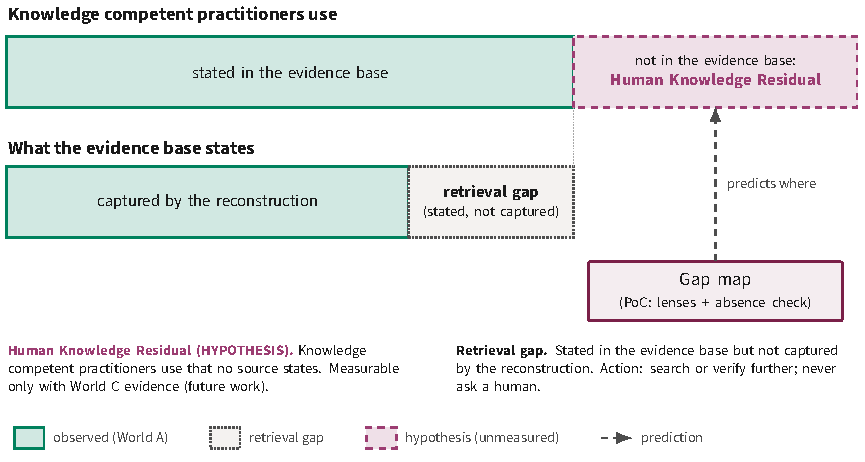
\includegraphics{figures/pdf/fig12_residual.pdf}
  \caption[The Human Knowledge Residual]{What is the Human Knowledge Residual, and how would it
    be measured? The reconstruction $R$ is drawn from a frozen evidence base $E$; validated human
    items $H$ come from elicitation and traces (World~C). The residual is the part of $H$ that $E$
    does not state; items that $E$ states but $R$ missed are reconstruction misses. Thinness is a
    property of $R$ alone. The gap map predicts, from $R$ only and before any human is asked,
    where the residual lies. Dashed elements are not built.}
  \label{fig:residual}
\end{figure}

\paragraph{What each study measures in place of the HKR.} \evint{} Only the prospective study (V5)
measures the construct as defined, and V5 decides H2. The others measure named proxies. In the
pooled CTA gold study (V2), published gold lists stand in for $H$: their items were elicited and
published, not re-validated by use. V2 therefore screens; it does not decide. The
developer-departure study (V3) measures realized knowledge loss after a departure (rationale-seeking
issues and defect-fix commits), predicted from coverage of code artifacts. That is a different
construct, so V3 tests a separate organizational hypothesis (H-OSS) and can neither support nor
refute H2 (\cref{sec:validation}).

\paragraph{Thinness is not the residual.} Three quantities must not be blurred. \emph{Thinness} is
a property of the ledger $R$ alone (source density, independent sources, retrieval gaps,
\code{UNKNOWN} slots, cross-run agreement); the PoC computed it for three ledgers. The \emph{HKR} is
a relation of $H$ to $E$, not yet measured. The \emph{gap-map prediction} is an area score,
$P(\mathrm{residual\ present} \mid \mathrm{area})$, labeled \code{inferred}; none is built yet.
On PLC the gap-map score tracks source density closely (\cref{sec:n3}). \evint{} An area can be thin
because retrieval was poor or because the knowledge is unwritten; only human evidence tells the two
apart. Hence density and area size are headline baselines in every test.

\subsection{How the residual would be measured}

\evfut{} The protocol reuses the registered rules of \repo{REORIENTATION.md} §14 and §18.
\begin{enumerate}[noitemsep]
  \item Freeze and hash-commit $E$, $R$, the area partition, the gap map and its area score before
    any human data exist.
  \item Elicit with a channel matched to the knowledge type: CDM-style retrospective probes for
    episode-specific cues \parencite{klein1989critical}, observation or traces for automated
    procedure, contrasting cases for perceptual cues. At least one arm stays blind to $R$.
  \item Segment transcripts into items at a grain fixed in a codebook.
  \item Validate each item by a second expert, a trace or an artifact outside $E$. Other experts
    rate importance later, blind to how the area was chosen.
  \item Match each item against $R$ and the frozen corpus, by blind coders or by a model matcher
    that meets the adoption rule (\cref{sec:validation}).
  \item Count per area and type.
  \item Estimate unseen items from text occasions only after a known-truth check against published
    gold (V4). Text occasions share authors and pretraining, so they underestimate stably
    \parencite{chao1987estimating,briand2000comprehensive}.
\end{enumerate}
A residual of zero is never reported. What makes this hard (incomplete gold, method-dependent
elicitation, matcher error, a moving evidence base) is treated with the program's threats
(\cref{sec:validation}).

\begin{evobsbox}
  The accounting types exist and refuse these shortcuts. \code{ResidualAccount} computes
  $H \setminus R$, $R \setminus H$, recall by type and $\mathrm{Res}_{\mathrm{obs}}$. It raises
  \code{ResidualNotMeasurable} when an item of $R \setminus H$ lacks a human validity judgment, and it
  rejects a non-human validity rater and a model matcher from the generator's family. No estimator
  is implemented, nothing produces the declared \code{GapMapPrediction} type, and no World~C data
  exist.\footnote{\repo{residual/src/residual/residual.py}.}
\end{evobsbox}

\paragraph{Why it would matter.} \evhyp{} If the HKR is non-trivial and measurable, each validated item of $H \setminus E$ can be
stored with its domain, knowledge type, revealing channel and pre-elicitation gap-map score
(\repo{REORIENTATION.md} §14.5). Across domains this \emph{residual corpus} would calibrate gap
maps, give CTA research a measure of omission relative to text, supply validated hidden steps for
instruction (\cref{sec:education}), and show which organizational units depend on people
(\cref{sec:organizations}). \evint{} A small residual would also be informative: there, expert time
belongs to verification, not elicitation.

\section{The validation program}\label{sec:validation}

This section designs the studies that would turn gap candidates into validated predictions of
where the Human Knowledge Residual lies (\cref{sec:residual}). \evfut{} Nothing in it has run. It
follows the rules registered in \repo{REORIENTATION.md} (§14, §18, §22) and marks anything new as
\enquote{proposed}. \evobs{} The starting point is a pipeline with one bottleneck. The absence
check (closure) is not yet informative: the judge's verdict does not depend on which evidence it
is shown. All three maps also share one configuration tuned on the same ledgers
(\cref{sec:n3,sec:not-demonstrated}).

The program asks for no money before its cheapest decisive test has run, and each tranche of money
is released only by a gate that reads CONTINUE. It has three phases (\cref{fig:validation}).
Phase~0 tests the absence check before any grant. Phase~1, a lean methods grant, screens the gap
map against several published expert golds. Phase~2 decides H2 with a blind prospective study
sized for the decision.

The studies test the hypotheses of \cref{sec:question} one link at a time; a failed link stops or
reroutes everything above it. The links are trustworthy inputs (L0, V0), an informative absence
check (L1, V1) and retrospective prediction on published gold (L2, V2). Then come a measurable
residual (L3, V4), prospective prediction (L4, V5, which decides H2) and practical value (L5,
V6--V8; V6 tests H3).
\evint{} L1 comes first: with an uninformative closure step, a gold test measures \enquote{a lens
fired} plus density. The developer-departure study (V3) is off this chain: it tests a separate
organizational hypothesis, H-OSS (\cref{subsec:hoss}), and can neither stop nor license H2.

\subsection{Phases, gates and the money they release}

\begin{evfutbox}
  \textbf{Gate rules, proposed for pre-registration.}\\[2pt]
  \textbf{MS1, closure verdict (end of Phase~0).} CONTINUE if human--human $\kappa \geq 0.70$ on
  the gating split, corpus-level retrieval recall meets its pre-registered floor, and at least one
  judge beats the fair control by the pre-registered margin. Otherwise STOP the automated absence
  check.\\[2pt]
  \textbf{MS3, screening gate for Phase~2 money (end of Phase~1).} CONTINUE only if the pooled
  retrospective $\Delta$AUROC has a point estimate $\geq \delta$, \emph{and} its lower 90\% bound
  is $> -\delta/2$, \emph{and} the map adds value over density and area size. Otherwise STOP H2
  funding. MS3 is not a verdict on H2, and it has no inconclusive route: it releases Phase~2 or it
  does not.\\[2pt]
  \textbf{MS5, H2 verdict (Phase~2).} STOP if the upper 90\% bound of the prospective
  $\Delta$AUROC is below $\delta$. CONTINUE if the lower 90\% bound is above 0 and the point
  estimate is at least $\delta$. Any other reading is inconclusive, is reported as not supporting
  H2, and ends H2 funding.
\end{evfutbox}

\paragraph{Phase~0: the closure study, before any grant.} \evfut{} This is the recommended next
action. The owner runs V1 within the NOW program's one permitted human input: a non-owner blind
coder who labels and does not participate. It needs no participants, no gold and no grant: coder
hours and local compute, of the order of EUR~$10^3$. \evint{} Its numbers (human--human $\kappa$,
retrieval recall, and each judge's own-minus-control gap) should be on page~1 of any grant
proposal; this report is the design for them. On STOP, the program takes one of two pivots:
reconstruction with provenance as an audit tool, with no claim about hidden knowledge, or the
interview-only pivot (\cref{sec:roadmap}).

\paragraph{Phase~1: a lean methods grant, released only on MS1 CONTINUE.} About EUR~0.3--0.5\,M
over 12--15 months (\cref{sec:resources}). It builds the area score and freezes the
configuration (MS2). It then validates the adopted judge on the text type of the later studies,
runs V2 pooled over several published CTA golds with V4 on the same data, and ends at MS3. On STOP, H2 funding ends; the
interview-only pivot is costed separately and must stand on its own merits. If H2 fails here, the
money spent on it is Phase~0 and Phase~1 only.

\paragraph{Phase~2: the full program, released only on MS3 CONTINUE.} V5 decides H2 at MS5 and is
budgeted for the power its rule needs. V6 (H3), V7 and the novice study V8c start only on MS5
CONTINUE, each under its own gate. H-OSS (V3) runs on the organizational track once its
components exist.

\paragraph{Who reads the gates.} An independent statistician, or an advisory board with one, reads
MS1, MS3 and MS5 against the pre-registration, with authority over them; any owner exception needs
this reader's sign-off. \evobs{} The N2-to-N3 step was an owner exception without such a reader
(\cref{sec:evolution}), and none is named yet (\cref{sec:team}).

\subsection{Rules common to every study}

\paragraph{Pre-registration and a two-step freeze.} \evfut{} Every threshold, the primary gold,
model and baseline, the area partition and the gap-map configuration are hash-committed before the
data they judge exist \parencite{nosek2018preregistration}. The order is fixed. First, the judge is
chosen at MS1. Then MS2 (about month~4 of Phase~1) hash-commits the V0, V2 and V4
pre-registrations, the lexicons, the thresholds, the adopted judge, the area score and the list of
eligible golds. Only then is gold acquired, and only then are held-out domains reconstructed. A
change after gold is seen makes the result exploratory. H-OSS has its own freeze (MS2b), after its
Git adapter exists.

\paragraph{Area score.} \evobs{} The gap map emits claim-level candidates, cut by a display cap
that drops most PLC candidates, and no area score (\cref{sec:n3}). \evfut{} Every decisive test
ranks \emph{areas}, so Phase~1 builds an area score before MS2. It is a fixed aggregation (for
example the maximum, or a noisy-OR) of per-candidate scores over the \emph{uncapped} lens records in
each area of the registered partition, with a tie rule. It is chosen on pilot data only. Proposed: a map with
more than half its areas tied at zero is uninformative for that gold.

\paragraph{Density and area size.} \evint{} Candidacy and rank are built from source counts, and on
PLC the ranking tracks source density ($\rho = 0.91$, \cref{sec:n3}). A plain $\Delta$AUROC over
density is then close to testing a variable against itself, and a null would be expected by design.
\evfut{} So, before MS2, the area score's partial rank correlation with density and area size is
reported on the pilot ledgers, and the incremental analysis is pre-registered. Primary: the area
score's AUROC \emph{within} density tertiles, pooled over tertiles and golds (the conditional
AUROC). Secondary: the area score's coefficient in a logistic model that already contains density
and area size, with gold as a random intercept.

\paragraph{Domains, dated corpora and memorization.} PLC and GDPR tuned the lexicons, so they serve
only for debugging, the V1 closure set and an unanalyzed V5 pilot. Decisive studies use held-out
domains on a corpus dated before the criterion (\cref{sec:domains}). \evfut{} A dated corpus admits
only sources with a verified date. These are archive captures (Wayback Machine CDX records or
Common Crawl snapshots) taken before the cutoff and used as captured, and publications whose
OpenAlex publication date precedes it. A per-gold blocklist removes the gold paper and its known
citing works. Older procedural text is often paywalled, so before MS2 a metadata-level pilot counts
the dated sources each candidate gold's queries reach; below a pre-registered floor, the gold is not
eligible. \evint{} Memorization cannot be removed: every model postdates the old golds, including
the planner that picks queries. The area partition therefore comes from a dated pre-gold source
by a written procedure, not from a model. Each gold item gets a guided-completion memorization probe
on every model in the chain, and probe-positive items leave the primary analysis
\parencite{golchin2023time,sainz2023nlp}. A plain-LLM ranking without retrieval is a baseline, so
priors alone are scored.

\paragraph{Judges and matchers.} No LLM judge is a criterion. A judge or matcher is adopted only
from a family other than the generator's, with $\kappa \geq 0.70$ against blind human coders and
not below the lower bound of human--human $\kappa$ (the adoption rule). \evfut{} Proposed: before
any gold is unsealed, a stratified sample of closure units from each dated V2 reconstruction, and
later from each V5 domain, is double-coded. Where the adopted judge fails the rule on that text
type, closure there is human-coded, a pre-registered fallback rather than a configuration change.

\paragraph{Statistics.} The headline metric is area-level AUROC, compared by DeLong's method
\parencite{delong1988comparing}, Obuchowski's clustered extension
\parencite{obuchowski1997nonparametric} or a cluster bootstrap. \evfut{} Proposed: the strongest of
the pre-specified baselines is chosen \emph{inside each bootstrap resample}
($\min_k \Delta\mathrm{AUROC}_k$), so the choice is part of the sampling distribution. The MS5 rule
has the logic of two one-sided tests
\parencite{schuirmann1987comparison,lakens2017equivalence,lakens2018equivalence}. Labels use
weighted $\kappa$ or Krippendorff's $\alpha$ \parencite{hayes2007answering,krippendorff2004reliability},
with prevalence beside $\kappa$ \parencite{feinstein1990high} and Wilson intervals
\parencite{wilson1927probable}.

\paragraph{Choosing $\delta$, and planning arithmetic.} \evfut{} Proposed: $\delta = 0.05$ AUROC
(still open in the registered threshold table). A smaller gain over density is unlikely to justify
the reconstruction, while $\delta = 0.10$ would let a stop rule kill a real but modest gain.
Planning uses Hanley--McNeil errors \parencite{hanley1982meaning}, balanced classes, AUROC 0.70
against 0.62 and an error correlation of 0.5; \evint{} these values have no empirical basis. The
90\% half-width of $\Delta$AUROC is then about $\pm 0.14$ with 20 areas per class, $\pm 0.10$ with
40, $\pm 0.08$ with 60, $\pm 0.06$ with 100 and $\pm 0.05$ with about 150. It depends mainly on the
number of areas: a smaller gap (0.66 or 0.62 against 0.62) moves it by under 0.01, and a
correlation of 0.3 widens it by about a fifth. One CTA gold, such as Sullivan's 46-item list
\parencite{sullivan2014use}, gives perhaps 15--25 areas.

\subsection{The studies}

\Cref{fig:validation} shows the phases and gates; \cref{tab:validation} summarizes each study.

\begin{figure}[tbp]
  \centering
  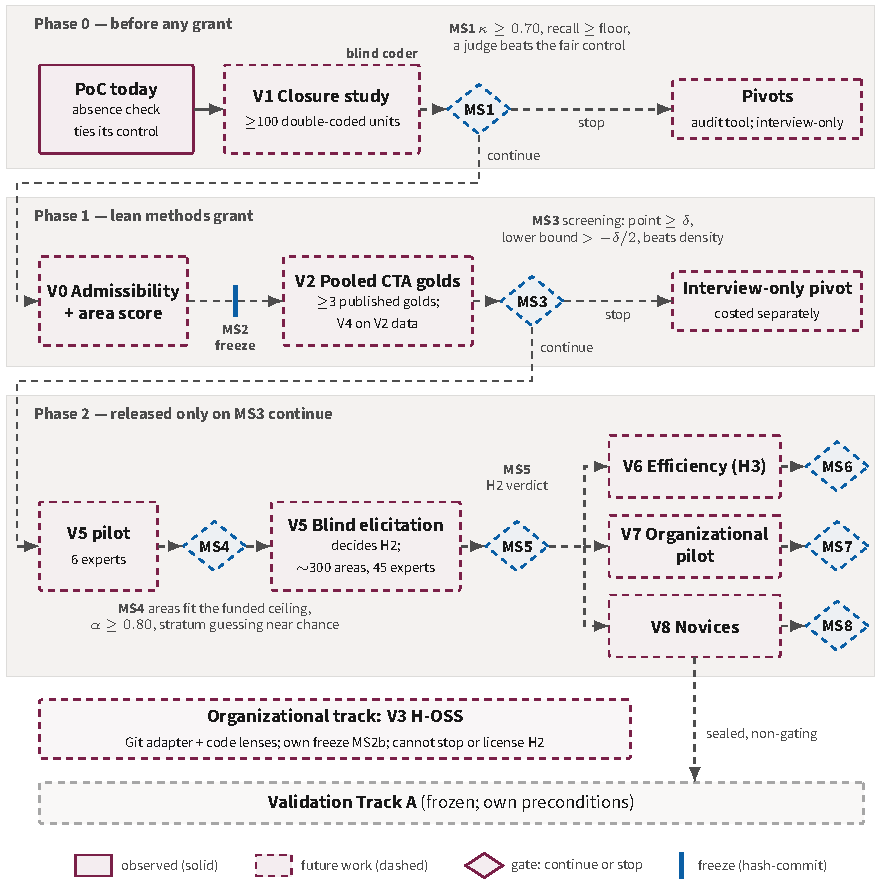
\includegraphics{figures/pdf/fig13_validation.pdf}
  \caption[The validation program]{Which studies, in which order, turn gap candidates into
    validated predictions, and which gate releases which money? Phase~0 (V1, the closure study,
    before any grant) ends at MS1. On CONTINUE, Phase~1 (V0 and the MS2 freeze, V2 pooled over
    several published CTA golds, V4) ends at the MS3 screening gate, which either releases
    Phase~2 or stops H2 funding. In Phase~2, V5 decides H2 at MS5 (after its pilot gate MS4);
    only on CONTINUE do V6 (H3), V7 and V8 follow. V3 sits on the organizational track: it tests
    the separate hypothesis H-OSS and can neither stop nor license H2. A STOP at MS1 leads to
    one of two pivots (an audit tool, or interview-only); a STOP at MS3 leads to the separately
    costed interview-only pivot. Validation Track~A runs on a separate rail on its own
    preconditions and connects only through sealed, secondary, non-gating predictions. All
    elements except the PoC are future work.}
  \label{fig:validation}
\end{figure}

\subsubsection{Phase~0 --- V1 (L1): the closure study}

\emph{Labels and units.} Coders and judges assign \emph{closed}, \emph{partial} or \emph{open},
the three states triage uses. A unit is (lens, seed span, missing element, evidence pool), in the
two arms of the PoC's fair control: own evidence, and evidence swapped from the nearest other
candidate of the same lens. The sample is all 107 admissible PoC firings (PLC 56,
GDPR~v1 51)\footnote{\repo{research/n3/plc/gapmap.json} and the GDPR maps, key
\code{checks.judge_lexical_confusion}.} in both arms: 214 units, and at least 100 double-coded
units if some prove uncodable. About 100 units from one new non-gold domain are added, so that no
judge is scored only in-sample. GDPR~v2's 48 firings (not N3-admissible) serve only for codebook training.
\emph{Coders.} The judgment is textual, so coders need codebook training, not domain expertise. The
non-owner coder and the owner (under origin blinding) code every unit, blind to arm, judge answer,
rank and run. \evint{} The gating $\kappa$ therefore pairs one non-owner coder with the owner;
Phase~1 adds a second non-owner coder.
\emph{Retrieval recall.} \evfut{} The residual requires absence from the whole corpus, not only
from the retrieved pool. So, for a random subset of about 50 firings, the non-owner
coder searches the ledger's full fetched snapshots for the missing element. Retrieval recall is the
share of elements found there that the pool also holds; proposed floor 0.80.
\emph{Judges and measures.} The panel holds the local 7B model, a stronger open-weight model, and
frontier models from families other than the generator's and verifier's (proposed decision 0008).
Primary measure: agreement on the three states (weighted $\kappa$, or ordinal
Krippendorff's $\alpha$), with closed versus not closed, the triage split, as the gating split.
Secondary: the prevalence of \enquote{not stated}, and each judge's own-minus-control difference
against the humans'.
\emph{Sample size.} With classes near balance on the gating split, $\kappa \approx 0.70$ (observed
agreement 0.85, chance 0.50) has a 95\% half-width of about $\pm 0.10$ at 214 units and $\pm 0.14$
at 100. The open state is rare (the judge called 15 of 155 firings open), so its $\kappa$ is wide
at this size (about $\pm 0.17$ at 200 units); it is reported, not gated. Units share seeds, so
$\kappa$ intervals are clustered by seed.
\emph{Gate (MS1).} As in the box. Proposed margin: a judge beats the fair control if its
own-minus-control difference in the not-closed rate has a 95\% lower bound above 0 and lies within
$\pm 0.10$ of the humans' difference. The adopted judge must also meet the adoption rule on the
gating split, on the new domain alone as well as pooled.

\subsubsection{Phase~1 --- V0 (L0): readiness and the deferred N2 validation}

Prepare the MS2 freeze. Implement admissibility as code: every located extraction has a verdict,
the cross-family verifier and the decoys ran (their current stages never ran live;
\cref{sec:architecture}), and completeness comes from the failed-call record. Build the dated-corpus
mode and the area score. N2's registered verdict is INCONCLUSIVE (\cref{sec:n2}); its deferred
protocols (E-LIVE v3, second runs of E-PLANT and E-ABST) run as registered, after a pilot that
prints each gate's best reachable outcome. E-PLANT's validity floor is re-derived from that pilot,
as a registered amendment, because it came from a setting where the planted document was the only
retrieved context. \emph{Gate:} MS2; no hash, no gold. The deferred N2 validation gates V7 and any
provenance claim, not V2.

\subsubsection{Phase~1 --- V2 (L2): pooled replay against published CTA golds}

\emph{Golds and the selection rule.} \evfut{} A gold is eligible if it is an itemized list of
steps, decisions or cues, built by CTA from more than one expert. Its domain must also yield a dated
corpus above the floor and must not be PLC, GDPR or Track~A's physics content, and the gold must be
obtainable for coding. Eligibility is checked by metadata and author contact only,
and the list is fixed at MS2. Named candidates follow, in order. Sullivan's
cricothyrotomy task list is the only one confirmed as itemized \parencite{sullivan2014use}. Then
come the neonatal intensive-care (NICU) cue study \parencite{crandall1993critical}, the troubleshooting study
\parencite{chao1994percentage} and the PARI guide's worked analyses \parencite{hall1995procedural}.
Further CTA-based studies reported in reviews \parencite{clark2008cognitive,tofelgrehl2013cognitive}
have unchecked availability.
Proposed: at least three golds, four to six if eligible. Fewer is reported at MS2; the MS3 rule
does not change, so fewer areas only make CONTINUE harder.
\emph{Design.} For each gold, build the area partition from a dated pre-gold source and
reconstruct from the dated corpus, the gold domain's first and only reconstruction. Run the frozen
gap map and double-code the closure sample; only then acquire the gold, sealed. \evint{} The gold stands in for
$H$, and the reconstruction $R$ is not the evidence base $E$ (\cref{sec:residual}). So each gold
item that $R$ lacks is checked against the dated corpus under the V1 codebook. An area is
\emph{residual-present} only if it holds an important gold item absent from the corpus; items the
corpus states but $R$ missed are scored separately as reconstruction misses.
\emph{Baselines.} The registered baselines, among them random, area size, retrieval-support
density, corpus frequency, a type prior from the other golds (leave-one-gold-out), and a plain-LLM
ranking on a model from another family. Coders see no score, origin or model family; all
item-to-area assignments and at least 20\% of reconstruction--gold pairs are double-coded.
\emph{Analysis.} Primary: the pooled $\Delta$AUROC for residual-present areas against the strongest
baseline, by a random-effects model over golds or a cluster bootstrap with gold as the top-level
cluster. Incremental: the conditional AUROC within density tertiles; the map \enquote{adds value}
at MS3 if its point estimate is at least $0.5 + \delta$.
\emph{Sample size and what MS3 can read.} Three to six golds of 15--25 areas give about 45--150
areas. At four golds and 80 areas split evenly, the half-width is about $\pm 0.10$ before
between-gold heterogeneity. CONTINUE then needs a point estimate of at least 0.075, because the
lower bound must clear $-0.025$. Under the planning assumptions, a map with no true gain passes
with probability about 0.11. A true gain of $\delta$ passes with about 0.34, and one of 0.10 with
about 0.66 (0.13, 0.45 and 0.81 at 60 areas per class). \evint{} MS3 is a screen. It accepts
about a one-in-nine chance of releasing Phase~2 for a map with no gain, which V5 then stops, in
exchange for keeping most large gains. It cannot show that a small gain is absent; that is V5's
job.

\subsubsection{Phase~1 --- V4 (L3): the residual known-truth check}

First a labeled synthetic simulation with planted dependence between occasions (a known-truth use
of synthetic data, not a criterion). Then, on V2 data, capture--recapture estimators that allow
unequal catchability over text occasions are compared with the gold-as-occasion count against a
pre-set tolerance, with Chao1 as a lower bound \parencite{chao1987estimating,briand2000comprehensive}. \evint{} Literature is written by experts, so
occasions are positively dependent and the estimate is biased low; only the known-truth check can
validate it. Out of tolerance, the estimated residual is dropped as an objective and V5 reports
observed counts only. V4 informs MS3's report but does not gate it.

\subsubsection{Phase~2 --- V5 (L4): blind prospective elicitation, which decides H2}

\emph{Design.} Within-expert and area-level. Freeze and hash-commit the reconstruction, dated
corpus, gap map, area score and area partition. Sample areas into four labeled strata: top of the
area score (G), lowest retrieval density (D), top of a plain-LLM ranking (L) and uniform random
(R), plus a pre-registered fraction of confident-but-unverified areas
\parencite{lakkaraju2017identifying}. Sampling spans the whole score range, so $\Delta$AUROC is
estimable with known inverse-probability weights. Each area gets a short probe of about 8 minutes: the same neutral CDM-style question for every area
\parencite{klein1989critical} (\enquote{Walk me through the last time you handled this. What did
you notice? What did you check? What would a newcomer miss?}), never the gap map's own question,
and at most one follow-up restating the expert's words. Each expert covers about 20 areas in two
sessions, balanced across strata, in random order.
\emph{Domains and people.} A PLC pilot, not analyzed for effect; the main study in two held-out
domains with at least 150 areas each at the registered grain (\cref{sec:domains}). Practitioners
with several years of practice, outside any Track~A pool, three per area, the best cost--benefit
point in \textcite{chao1994percentage}. One interviewer per domain, two blind coders, one
validator.
\emph{Outcome.} Expert turns are segmented into items (cue, decision rule, check, rationale,
expectancy). An item counts if it is absent from the frozen reconstruction \emph{and} the dated
corpus under the V1 codebook, and a second expert, a trace or an artifact outside the corpus
corroborates it. Other experts rate importance a week later, blind to stratum. An area is
\emph{residual-present} if it holds at least one validated, important new item.
\emph{Blinding and disclosure.} Experts are told that the study maps where practice relies on
unwritten knowledge, not that a model chose areas. This partial disclosure is stated in the ethics
application; every expert is debriefed afterward and may withdraw their data. The interviewer sees
only area names in random order, coders see pseudonymized turns, and a guess-the-stratum check on
20\% of areas reports leakage.
\emph{Analysis.} Primary: prospective $\Delta$AUROC against the strongest baseline, clustered by
expert and area \parencite{obuchowski1997nonparametric}, with the conditional AUROC within density
tertiles. Secondary: the rate ratio of validated important items, G against the strongest of D, L
and R (mixed-effects negative binomial, \cite{bates2015fitting}), and expert minutes per item.
Segmentation targets $\alpha \geq 0.80$; \enquote{new versus in text} and \enquote{same item} need
$\kappa \geq 0.70$.
\emph{Sample size and expert-hours.} No effect is assumed. MS5 needs a half-width near
$\delta = 0.05$: about 150 residual-present and 150 other areas, so about 300 areas. Three experts
per area make 900 probes. At 20 areas per expert, that is 45 experts (about 22 per domain) plus 6 in
the pilot. Each expert gives about 3 hours in sessions and 1 hour rating other experts' items: about
150--250 expert-hours in all, and about 70 session hours per interviewer. \evint{} Coding costs
more than the experts. About 120 hours of audio must be segmented and matched against the
reconstruction and the dated corpus by two coders: about 1,200--1,900 coder hours. At the rates in
\cref{sec:resources}, honoraria, recruitment and coding come to roughly EUR~40--160k before staff
time. Two things can raise this. If residual-present areas are rarer than half, more areas are
needed (about 500 at a prevalence of 0.3), and clustering by expert adds a design effect.
\emph{Gates.} The pilot (6 experts $\times$ 20 areas: 40 areas, three experts each) estimates
prevalence, design effect, coding time and leakage. \textbf{MS4} releases the main study only if the
projected number of areas fits a funded ceiling of 450 (1.5 times the plan), segmentation reaches
$\alpha \geq 0.80$, and stratum guessing stays near chance. Otherwise V5 stops before the main
study, and H2 is reported as untested prospectively; an underpowered main study is never run.
\textbf{MS5} then reads the rule in the box. At a half-width of $\delta$, every reading is decisive
except a point estimate between 0 and $\delta$.

\begin{table}[tbp]
  \centering\scriptsize
  \caption{The validation studies at a glance. All rows are future work; every rule is
    pre-registered before the data it judges. \enquote{At planned $n$} gives the best reachable
    outcome under the planning arithmetic.}
  \label{tab:validation}
  \begin{tabularx}{\linewidth}{@{}>{\raggedright\arraybackslash}p{0.12\linewidth}
      >{\raggedright\arraybackslash}p{0.10\linewidth}>{\raggedright\arraybackslash}p{0.11\linewidth}
      >{\raggedright\arraybackslash}X>{\raggedright\arraybackslash}p{0.17\linewidth}
      >{\raggedright\arraybackslash}p{0.16\linewidth}@{}}
    \toprule
    Study (link) & Phase / gate & Humans & CONTINUE if & Otherwise & At planned $n$ \\
    \midrule
    V1 Closure (L1) & 0 / MS1 & Owner + 1 non-owner coder & Human $\kappa \geq 0.70$; recall
      $\geq$ floor; a judge beats the fair control by the margin & STOP automated absence check;
      pivots & $\kappa$ $\pm 0.10$ at 214 units \\
    V0 Readiness (L0) & 1 / MS2 & 1 coder (E-ABST) & Runs admissible; MS2 hash; N2 gates as
      registered & No hash: no gold; N2 Stop: no V7 & -- \\
    V2 Pooled CTA golds (L2) & 1 / MS3 (screen) & 2 coders & Pooled $\Delta$AUROC point $\geq
      \delta$, lower 90\% $> -\delta/2$; conditional AUROC $\geq 0.5 + \delta$ & STOP H2 funding;
      separate pivot & $\pm 0.10$ at 40 per class: point $\geq 0.075$ needed \\
    V4 Residual check (L3) & 1 & None & Estimate within tolerance of gold-as-occasion & Drop the
      estimated residual & -- \\
    V5 Prospective (L4; H2) & 2 / MS4, MS5 & 6 pilot + about 45 experts, 3 per area & Lower
      90\% $> 0$, point $\geq \delta$ & Upper 90\% $< \delta$: STOP H2; else not supporting H2 &
      $\pm 0.05$ at 150 per class: decisive unless $0 \leq$ point $< \delta$ \\
    V6 Efficiency (L5a; H3) & 2 / MS6 & 20--30 per domain (illustr.) & Lower 90\% $> 1$, point
      $\geq 1.25$ & Any other reading counts against H3 & Sized from V5 data \\
    V7 Organizational (L5b) & 2 / MS7 & 1 partner, 6--12 staff & G beats D and R in both parts &
      Legal block; not measurable & Descriptive only \\
    V8a Learner data (L5c) & 2 & None & Error excess over difficulty baselines & Null: residual
      $\neq$ learner difficulty & -- \\
    V8b--d Track~A; novices; instruction & Own; 2 / MS8; later & Track~A's own; 30--60 novices &
      K0--K2 unchanged, E-SEAL secondary; novice error excess & Registered rules; no excess & -- \\
    \midrule
    V3 H-OSS (org.\ track) & Org.\ track / MS2b, own gate & 2 coders & Clustered $\Delta$AUROC, MS5
      rule, on H-OSS only & H-OSS stopped; too few departures: descriptive & Set by the
      5-departure pilot \\
    \bottomrule
  \end{tabularx}
\end{table}

\subsubsection{Phase~2 --- V6 (L5a, H3): targeted elicitation efficiency}

Runs only on MS5 CONTINUE, never on an expert's V5 areas. \emph{Selectors, kept distinct.} Two
selectors run as separate arms: the PoC's breadth ranking, as built and frozen, and selection by
expected information gain (EIG) over the gap map \parencite{lindley1956measure,rainforth2024modern},
which is not built. Information-gain questioning has helped in games and preference elicitation
\parencite{piriyakulkij2023active,handa2024bayesian,choudhury2025bedllm}, but no study was found in
expert interviews. A replay without participants (E-EIG) fixes the primary selector before any V6
data. \emph{Design.} Within-expert crossover on matched area sets: block~A targeted
questions, block~B a standard unprompted-then-CDM interview, counterbalanced; proposed third arm, a
plain-LLM list. Items whose content first appears in a question are coded \emph{question-seeded}
\parencite{loftus1975leading} and count only if independently corroborated; Track~A's
leading-question guard is reused by copy. \emph{Measure and gate (MS6).} Validated important new
items per expert hour, ratio A/B for the primary selector; illustration 20--30 experts per domain,
sized from V5's data. CONTINUE if the lower 90\% bound exceeds 1 and the point estimate is at least
1.25. STOP if the upper bound is below 1.25. Any other reading counts against H3.
\evint{} The interview-only pivot reuses this design with EIG over the area partition crossed with
knowledge types and a type prior from the golds, without the reconstruction prior. It is a separate,
separately costed proposal, not a test of H3.

\subsubsection{Phase~2 --- V7 (L5b): organizational pilot}

\evfut{} Runs only on MS5 CONTINUE and after the deferred N2 validation, since partner documents
raise the stakes of prompt injection and false support \parencite{greshake2023not}. In one partner,
it asks whether predicted gaps in critical units match what 6--12 staff experts add in blind
interviews, and where departures or onboarding caused trouble (\cref{sec:organizations}). It runs in
artifact-coverage mode only, under a data-protection impact assessment and, where German
co-determination applies, a works agreement. It reuses the V5 design on one or two units and, if
H-OSS has run, its retrospective design. \evint{} One partner cannot validate a predictor: the pilot
tests feasibility, legal viability and measurability, with the hit rate of G against D and R areas
as a descriptive measure. It goes multi-partner only if G beats D and R in both parts (MS7).

\subsubsection{Phase~2 and later --- V8 (L5c): the learner side, and how Track~A fits}

\evfut{} (a)~In public school-mathematics data, do flagged knowledge components carry more errors
than covered ones, beyond the dataset's own model \parencite{cen2006learning}? It needs no
participants and gates nothing; a null is likely, since the map reads expert-voiced text.
(b)~Validation Track~A runs only on its own preconditions, with K0, K1, K2 and Stage~B unchanged.
The program touches it only through sealed, secondary, non-gating predictions (E-SEAL): an
encrypted, hash-committed file, unsealed after K1 adjudication is locked and matched by coders with
no Track~A role. Anyone who has seen reconstructed conservation content stays ineligible for a
Track~A human role. (c)~On MS5 CONTINUE,
30--60 novices test whether confirmed residual areas show more novice errors than matched covered
areas (MS8). (d)~Much later comes instruction from validated items only, with delayed transfer
(\cref{sec:education}), where CTA-derived instruction has precedent
\parencite{feldon2010translating}.

\subsubsection{Organizational track --- V3: the separate hypothesis H-OSS}\label{subsec:hoss}

\emph{Hypothesis (H-OSS).} The gap map, adapted to code and commit evidence, predicts where
knowledge is lost when developers leave, beyond authorship concentration. \evint{} This is a
different construct from the HKR, measured with a different gap map. So H-OSS can neither stop
nor license H2, and its result is reported only as a reading on H-OSS.
\emph{Components (none exists).} (i)~A World~B Git adapter that turns commits, issues, pull
requests, reviews and dated documentation into claim records with exact spans keyed to a commit
hash or URL. (ii)~Areas mapped to code units existing at a time $t$ before
the departure. (iii)~Lens rules for code text; for example, WHY fires on a change whose commit, pull-request
and issue text give no reason, and GUARD on a special-case branch whose comment or commit names no
condition. Code-text lexicons are developed on repositories outside the
departure sample. The judge is validated on commit and issue units from such repositories; if none
passes, H-OSS is registered without closure (lens firing plus coverage only), a narrower claim.
All of this is frozen at MS2b, after the adapter exists.
\emph{Design.} As registered. Freeze each repository at $t$ and compute the adapted map from
artifacts dated no later than $t$. The outcome is blind, double-coded rationale-seeking
issues and defect-fix commits per unit of later activity, as a difference-in-differences with a
staggered-adoption estimator \parencite{callaway2021difference}. Departures come from truck-factor corpora
\parencite{avelino2016novel,avelino2019abandonment}. Baselines: prior trouble, size, churn,
documentation density, truck factor, knowledge at risk from turnover-loss studies
\parencite{rigby2016quantifying,nassif2017revisiting}, and a plain-LLM ranking. Blind outcome
coders reach $\kappa \geq 0.70$ on 200 stratified issues. Developers are pseudonymized data
subjects.
\emph{Sample size and gate.} The effective sample is near the number of departures. A 5-departure
pilot estimates the base rate, the within-repository correlation and coding time, and from them the
departures needed for a clustered 90\% half-width no wider than $\delta$. The main study runs only
if that many departures with enough later activity exist (the registered expectation is tens);
otherwise H-OSS is descriptive. Its own gate uses the MS5 rule.

\subsection{Threats to the validity of the program, and mitigations}

Contamination and in-sample tuning are treated with the PoC's threats (\cref{sec:threats}). Four
threats are specific to measuring the residual.

\paragraph{The gold is incomplete.} $H$ is what a few experts said and did, so true residual items
outside it look like false positives. Hence three experts per area as a floor
\parencite{chao1994percentage}, $R \setminus H$ reported but never as error, saturation checks that
allow for plateaus \parencite{guest2020simple,hennink2022sample}, and no residual declared zero.

\paragraph{The method shapes $H$.} Prompting changes how much experts report (\cref{sec:problem}),
verbal reports can be wrong \parencite{nisbett1977telling}, directed explanation can change what
experts do \parencite{fox2011procedures,ericsson1980verbal}, and leading questions can plant content
\parencite{loftus1975leading}. The measured HKR is always \enquote{the residual as revealed by
method $M$}, a lower bound, and V5's short probes make it a conservative one. Hence neutral probes,
question-seeded coding and corroboration.

\paragraph{The matcher can err or become the gold.} A lenient matcher shrinks the residual, a
strict one inflates it, and an unchecked LLM matcher silently becomes the criterion. Hence the
adoption rule and its re-check on each text type, matchers blind to scores and origin, and
contradicted items recorded as contradictions. Results compare only at a fixed, dated $E$.

\paragraph{People and governance.} A frozen codebook, origin blinding, non-owner gating coders and
random area order guard against drift, owner knowledge and fatigue. With one interviewer per domain,
the claim is \enquote{with this interviewer}.
Ethics approval covering V5's partial disclosure precedes V5; an impact assessment and a works
agreement precede V7. A study stopped by budget or law is reported as stopped, never
reinterpreted.

\evint{} Each STOP teaches something. At MS1, it shows that absence in text cannot yet be judged
reliably, and it leaves a public closure set. At MS3, it leaves a reconstruct-versus-CTA benchmark.
At MS5, it falsifies the claim that text reconstruction locates the human residual, with a bounded
effect size.

\section{The proposed platform}
\label{sec:platform}

This section describes a platform that does not exist. It is the target the proof of concept
(PoC) is one walking skeleton toward, drawn from the design already latent in the PoC's code and
decisions (\repo{docs/architecture/decisions}). Almost everything in this section is
\textsc{future work} \evfut. Every component below states its own status; a status tag of
\textsc{implemented in poc} names the file that exists today, and nothing else in this section
should be read as built. The PoC has no human validation. The gap map in
\cref{sec:n3} produces gap candidates, not identified tacit knowledge, and nothing in this
platform design changes that: a gap candidate remains a prediction until a human answers it.

\subsection{Three evidence worlds}
\label{sec:platform-worlds}

The platform organizes every piece of evidence into one of three worlds, already a typed field
in the PoC's code: \code{World.A = "public"}, \code{World.B = "organisational"},
\code{World.C = "human"} (\repo{residual/src/residual/vocab.py}) \evobs. A world is defined by
which body of evidence a source belongs to, not by how it was accessed. A public learner-response
dataset is World A even though a school collected it, and an open-source project's own commit
history is World B even though the repository is public.

\paragraph{World A --- public evidence.}
Textbooks, papers, standards, guidance, forums, task analyses, and public learner-response
datasets. It can yield concepts, taxonomies, taught heuristics, and cohort-level difficulty
\evint, but not episode-specific cues or organization-specific practice, since those are not
written down for the public. \evobs{} Implemented for open-web text only, in the two live N3
domains; no curated tier yet (every source is host tier \code{"open"}, decision 0007). Public
learner datasets are not ingested (N4, \textsc{next research stage}).

\paragraph{World B --- organization-specific evidence.}
Standard operating procedures (SOPs), wikis, tickets, commits, review threads, logs, incident reports, and design records
(\repo{residual/src/residual/vocab.py}) \evobs. World B carries a second axis World A does not
need, \emph{practice}: \code{imagined} (an SOP prescribes), \code{done} (a log records), or
\code{reported}; the gap between imagined and done is the organizational form of the residual
\evhyp. The schema exists \evobs; no ingestion does. The only planned adapter is a Git-history
adapter over \emph{public} repositories for the H-OSS study (V3, \cref{subsec:hoss}), \textsc{next research stage}; customer or
employee data is \textsc{long-term}, gated on a DPIA (\cref{sec:platform-nfr}).

\paragraph{World C --- human evidence.}
Expert elicitation, ratings, learner responses, and blind-coder labels. The types are \evobs{}
implemented (\repo{residual/src/residual/residual.py}), but no World C data exist in any
zero-participant NOW track. The frozen Validation Track A instrument (\repo{instrument/}) can
produce World C evidence and is built, but runs on its own preconditions, independent of this
platform (\cref{sec:validation}).

\paragraph{How the worlds interact.}
The cost order is A before B before C, because eliciting a human is the most expensive and
slowest evidence to collect, but information is not one-way. A and B build the reconstruction:
each claim is bound to a verified span, labeled \code{literature_supported} or
\code{organisational_artefact_supported} only after cross-family verification \evobs. B checks A,
and \code{done} checks \code{imagined}, producing contradiction records rather than a silent merge
\evfut. The gap map then predicts where World C is needed, over the reconstruction only, labeling
every output \code{inferred}: a predictor, never a criterion (decision 0008 (proposed), rule
\code{gap-candidates-are-predictors}) \evobs. World C answers through the channel matched to the
predicted knowledge type; validated answers form gold set $H$, and the observed residual is
$H\setminus R$ over $H\cup R_{\mathrm{valid}}$ (\cref{sec:residual}), the criterion the gap map is
scored against \evfut. World C feeds back in exactly two places: a validated item enters the
residual corpus carrying its pre-elicitation gap-map score, and a human verdict can raise a claim
to \code{observed_human_evidence}. World C never edits the reconstruction in place, since
reconstruction, gold, and surrogate material live in separate ledgers by \code{Ledger.purpose}
\evobs{} for the ledger separation, \evfut{} for the feedback itself. Finally, at least one human
arm must stay blind to the reconstruction, or anchoring will shrink the measured residual --- an
architectural constraint on the elicitation service, not a policy note \evfut.

\begin{figure}[tbp]
  \centering
  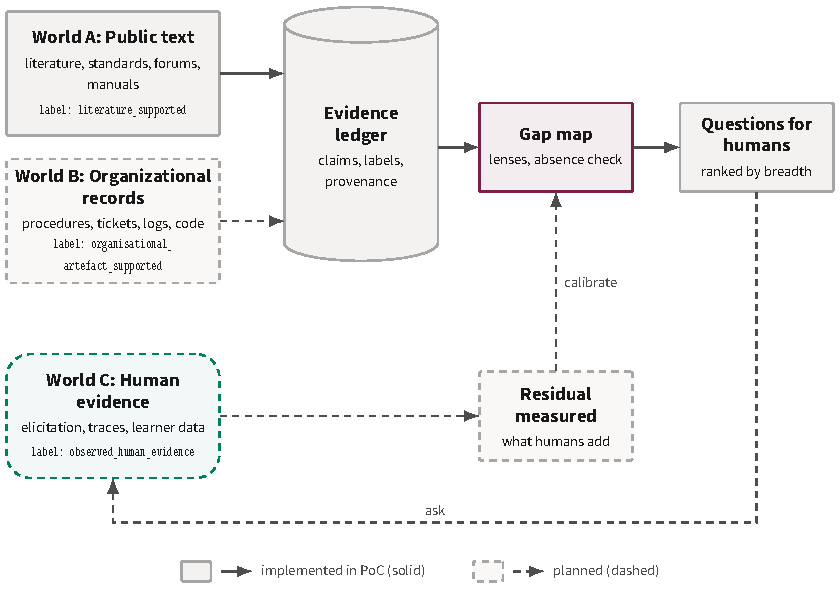
\includegraphics{figures/pdf/fig10_worlds.pdf}
  \caption[The three evidence worlds]{How public (A), organization-specific (B), and human (C)
    evidence interact. A and B build the reconstruction and the ledger; the gap map runs over the
    reconstruction and emits predictors; World C answers targeted questions and is the only path
    that can score those predictors, feeding back into the residual corpus that calibrates the
    next gap map. Solid arrows exist in the PoC; dashed arrows are future work.}
  \label{fig:worlds}
\end{figure}

\subsection{How evidence labels propagate}
\label{sec:platform-labels}

The six epistemic labels are defined in \cref{sec:evidence-model}. Four rules govern how a label
may move, all already enforced in the PoC or proposed as a direct extension of it:

\begin{itemize}[noitemsep]
  \item \textbf{Labels are computed, never set.} \code{ClaimRecord.label} is a property computed
    from a claim's evidence, not a field an author can assign (decision 0006) \evobs.
  \item \textbf{A label is only as strong as its weakest required link.} A claim is
    \code{literature_supported} only with a located span \emph{and} a cross-family
    \textsc{supports} verdict; a fabricated quote yields no evidence and the claim stays synthetic
    (decision 0007, rule \code{span-is-ours}) \evobs.
  \item \textbf{Derived outputs are \code{inferred} at best.} Gap records, gap-map scores,
    generated questions, recovered organizational rationale, and any domain-model edge a model
    proposes are \code{inferred} or \code{synthetic_extrapolation}, never higher \evobs{} for gap
    records (decision 0008 (proposed), rule \code{gap-candidates-are-predictors}), \evfut{}
    elsewhere. An evidential gate refuses a synthetic, inferred, or unknown
    criterion outright (\repo{residual/src/residual/gates.py}, decision 0006, rule
    \code{synthetic-never-a-gate-criterion}) \evobs.
  \item \textbf{Labels move up only through World C or cross-family verification, and World B
    labels stay inside their organization.} A human verdict can raise a claim to
    \code{observed_human_evidence}, and an \code{organisational_artefact_supported} claim must
    never leave its organization's tenant. Both rules have their types in the code today; neither
    is enforced yet \evfut.
\end{itemize}

\subsection{Components of the platform}
\label{sec:platform-components}

\Cref{tab:components} lists the platform's components. A status of \textsc{implemented in poc}
names the code that exists; \textsc{next research stage} names work planned inside the NOW
program (\cref{sec:roadmap}); \textsc{long-term} names work that depends on an organizational
partner, learner data, or a validated criterion that does not yet exist.

\begin{footnotesize}
\begin{longtable}{@{}p{0.17\linewidth}p{0.26\linewidth}p{0.24\linewidth}p{0.24\linewidth}@{}}
  \caption{Platform components: responsibility, status, and main technical risk. Component detail
    is in \repo{report/notes/06_platform.md}.}
  \label{tab:components}\\
  \toprule
  Component & Responsibility & Status & Main technical risk \\
  \midrule
  \endfirsthead
  \toprule
  Component & Responsibility & Status & Main technical risk \\
  \midrule
  \endhead
  \bottomrule
  \endfoot
  Reconstruction pipeline &
    Plan searches, fetch, extract claims bound to spans, hand off to verification &
    \evobs\ Walking skeleton, \repo{reconstruct/src/reconstruct/run.py} &
    Retrieval set by generator family; extraction truncation dropped sources once; validation
    deferred \\
  Evidence ledger &
    Single typed contract between stages: claims, evidence, sources, verifications,
    contradictions &
    \evobs\ \repo{residual/src/residual/ledger.py}; schema hash-frozen in
    \repo{residual/frozen/n1.json} &
    Run sidecar is a second, untyped contract; one JSON file per run does not scale to an
    organization's corpus \\
  Provenance verification &
    Every span a slice of fetched, hashed text; cross-family support verification; independence
    clustering &
    \evobs\ Open web only, \repo{reconstruct/src/reconstruct/evidence.py} &
    Decoy validity self-certified; short derived copies escape duplicate detection \\
  Contradiction analysis &
    Find claims that conflict across sources and worlds (A vs.\ B, imagined vs.\ done) &
    \textsc{Next research stage}: an older pairwise stage ran in the v1 runs; the current
    cross-verify stage is coded but has never run live (\repo{residual/src/residual/ledger.py},
    \cref{sec:n2}) &
    Scope-flagged contradictions can read as false conflicts; the detector must not be the
    generator \\
  Domain learning model &
    Hold the domain as a layered composite, not a single ontology &
    \textsc{Next research stage} / \textsc{long-term}. Only layer and knowledge-type enumerations
    exist &
    Prerequisite, causal, and procedural edges are not reliably recoverable from text alone \\
  Methodology-guided gap detection &
    Fire lenses where sources attest a construct but not its content; judge closure; emit gap
    candidates and retrieval gaps &
    \evobs\ Candidates only, \repo{gapmap/src/gapmap} &
    Closure judge uninformative: own rate equals mismatched-evidence-control rate on every ledger
    (\cref{sec:n3}) -- decides the program \\
  Company retrieval (World B) &
    Acquire organizational artifacts with dates, authorship, access rights, as fetchable,
    hashable text &
    \textsc{Next research stage} (public Git) / \textsc{long-term} (customer data). Nothing built &
    Access control ignoring per-user rights leaks data; injection via tickets/chat worse than via
    web pages \\
  Expert elicitation &
    Ask experts the gap map's questions by channel matched to knowledge type; one arm stays blind &
    \textsc{Long-term} for new tracks. Track A's instrument is frozen (\repo{instrument/}), reused
    only by copy &
    Anchoring on the reconstruction; an AI interviewer leading the expert; channel mismatch \\
  Human Knowledge Residual measurement &
    Recall of validated human answers against the reconstruction; unseen-item estimate with a
    known-truth check &
    \textsc{Next research stage}. Types exist; no estimator, no gold acquired &
    Never-written items are invisible to text checks; the matcher can become the gold it tests
    against \\
  EIG question selection &
    Choose the next question by expected information gain, reserving a fraction for
    confident-but-unverified areas &
    \textsc{Next research stage}. Current ranking is a breadth rubric, not information gain &
    No prior study applies EIG to expert/CTA interviews; adaptive selection breaks the
    equal-catchability assumption \\
  Learner diagnostics &
    Build bottleneck hypotheses from learner responses &
    \textsc{Long-term} (own data) / \textsc{next research stage} (public data). Vocabulary only &
    Synthetic learners are negative evidence for this role (\cref{sec:education}); AI Act
    Annex~III obligations \\
  Instructional design &
    Turn validated residual items into worked tasks and practice &
    \textsc{Long-term}. Nothing exists &
    Teaching an unvalidated candidate would teach a prediction as a fact (\cref{sec:education}) \\
  Adaptive learning &
    Sequence practice per learner from a learner model &
    \textsc{Long-term}. Out of scope for now &
    Unguarded model-generated help can raise assisted while lowering unassisted performance
    \parencite{bastani2025generative} \\
  Validation loops &
    End every stage in a pre-registered, code-computed continue/change/stop decision &
    \evobs\ Gates and checks exist; gold tests are \textsc{next research stage} &
    A threshold's registration source is free text, not enforced; several thresholds unset \\
  Run ledger and cost tracking &
    Log every model/search call, including failures, with cost and served-model checks &
    \evobs\ \repo{reconstruct/} per-run \code{calls.jsonl} &
    Cost per \emph{validated} item not yet tracked; needs World C \\
\end{longtable}
\end{footnotesize}

\begin{figure}[tbp]
  \centering
  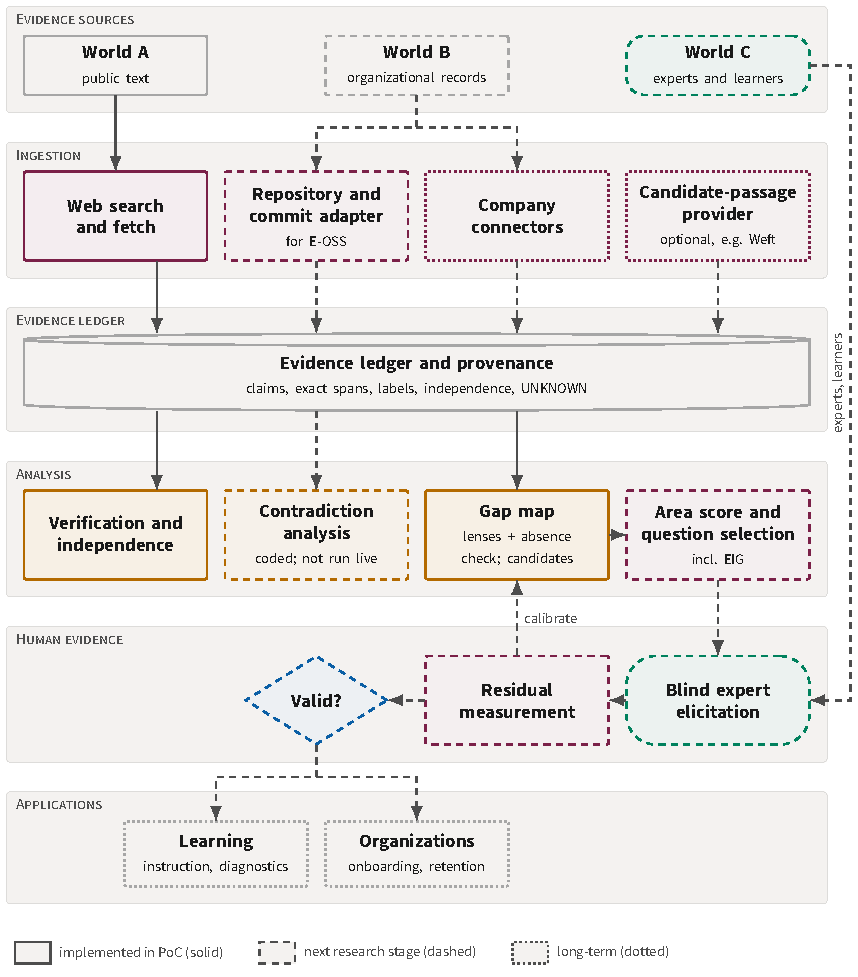
\includegraphics{figures/pdf/fig11_platform.pdf}
  \caption[Platform layers]{The platform drawn as layers, from evidence sources through
    acquisition, provenance, the evidence ledger, analysis, the human loop, and applications, with
    validation, audit, and security as a rail touching every layer. Solid boxes exist in the PoC;
    dashed boxes are the next research stage; dotted boxes are long-term. Every acquisition path
    passes through provenance before it reaches the ledger; only World C evidence can score the
    gap map's predictions.}
  \label{fig:platform}
\end{figure}

\subsection{Key architectural decisions}
\label{sec:platform-decisions}

Five decisions carry the platform's main design bets, drawn from
\repo{docs/architecture/decisions}. Two are already enforced in code: the evidence-ledger contract
and the synthetic-never-a-criterion gate. The three-model-family rule is followed today but checked
by code review, not by a test. The typed sidecar and the rule that unvalidated candidates never
reach a learner or end user are future work, the fifth adopted here for every application layer
that does not yet exist. Decision 0008, which the model-family and gap-candidate rules below draw
on, carries \code{status: proposed} in its own record.

\paragraph{The evidence ledger is the single contract between stages.}
Producers write typed records; consumers read them, and nothing else, so stages can be swapped or
re-run without touching each other. \evobs{} The core evidence package depends only on
\code{pydantic} (decision 0006, rule \code{residual-core-provider-neutral}). \evint{} One caveat:
the gap map also reads the reconstruction run's untyped JSON status sidecar, a second, informal
contract next to the ledger.

\paragraph{The run sidecar becomes a typed record.}
The platform closes that caveat by promoting run status into a schema with the same guarantees as
the ledger: versioned, hash-checkable, readable without re-deriving it from a log. \evfut.

\paragraph{Synthetic output may be a predictor, never a criterion.}
An evidential gate refuses a synthetic, inferred, or unknown label as the criterion side of any
measurement (decision 0006, rule \code{synthetic-never-a-gate-criterion}) \evobs. This is the
platform's main defense against a system that quietly grades its own predictions --- and why
\cref{sec:education} insists that only human-validated claims may reach a learner.

\paragraph{Three distinct model families for generator, verifier, and closure judge, on premises.}
The generator and verifier must come from different model families (decisions 0006, 0007) \evobs,
and the closure judge must differ from both again (decision 0008 (proposed)) \evobs. On-premises
deployment therefore needs three model families available locally, not one strong model reused
three times. The PoC already runs its closure judge locally (Ollama \code{qwen2.5:7b-instruct})
\evobs, showing the pattern is viable and, at the same time, its risk: that 7B judge did not beat
its mismatched-evidence control on any of the three PoC ledgers (\cref{sec:n3}).

\paragraph{Unvalidated candidates never reach a learner or an end user.}
A gap candidate is \code{inferred} by construction (decision 0008 (proposed), rule
\code{gap-candidates-are-predictors}) \evobs, and every application layer may only draw on claims
labeled \code{observed_human_evidence} or otherwise criterion-supported. \evfut{} No code enforces
this second part yet; it binds every future application layer.

\subsection{Non-functional requirements for organizational deployment}
\label{sec:platform-nfr}

Every requirement below is \evfut{}, stated as an extension of a property the PoC already has,
where one exists. Privacy, GDPR, and works-council requirements are stated once, in
\cref{sec:org-ethics}, and apply here unchanged; legal points there are the reorientation's own
reading of applicable law, not independently verified legal advice.

\paragraph{Security.}
Retrieved text is data, never instructions: the planner never sees artifact text directly,
extractors get no tool access, and injection-pattern spans are flagged and held pending rather
than acted on. This is already a rule for World A (decision 0007, rule
\code{retrieved-text-is-data}), extended to World B, where ticket and chat content is a stronger
injection vector than public web pages. Connectors use read-only, per-repository or per-space credentials, and any retrieval
substrate that runs third-party plugins in-process needs a pinned, reviewed allow-list, because an
in-process plugin runs with the adapter's own credentials to the organization's data
(\cref{app:weft}). One configured model backend per role, with a served-model check on every
response and no silent fallback list, holds for on-premises models exactly as it does today for
hosted ones (decision 0007).

\paragraph{Access control.}
Retrieval must enforce per-user access rights, and a claim inherits the most restrictive access
level of its supporting evidence. A gap map computed over restricted evidence is itself
restricted. World B claims never cross from one organization's ledger into another's, or into the
cross-organization residual corpus, without an explicit, contractual release and
de-identification. A reader without access to a claim's only supporting span must see that claim
as \code{unknown} for them, not as supported --- no type in the current schema expresses this yet.

\paragraph{On-premises models and audit trails.}
Organizational artifacts often cannot leave the premises they were created on. As
\cref{sec:platform-decisions} states, this requires at least three model families available
locally, one each for generation, verification, and closure judgment, following the pattern
already running for the N3 closure judge. Every model verdict is cached with its prompt hash and
replayed by default (decision 0008 (proposed), rule \code{gapmap-replays-by-default}), which
doubles as an audit and air-gapped-review mechanism. The PoC already logs every model and search
call, including failures, with the served model and its cost, snapshots that are
content-addressed, an offline re-slice of every evidence item, and a frozen schema and set of
prompt hashes (\repo{reconstruct/src/reconstruct/run.py}) \evobs. The platform adds: who viewed or
exported which gap map, which human verdict changed which label and when, and retention and
erasure events, all appended to a tamper-evident, hash-chained log. Cost headroom, including the
lesson the PoC's own budget stop taught, is stated once, in \cref{sec:resources}.

\subsection{Weft: a candidate substrate, not a dependency}
\label{sec:platform-weft}

Weft is a separate, public, MIT-licensed retrieval engine examined for this report as a possible
future World B acquisition layer; edu\_proj does not use, depend on, or integrate with it today.
It indexes a directory of text and PDF files with a content hash and a computed lineage. But it
keeps no in-document character offsets and no per-user access control, so any future adapter would
have to re-hash and re-locate every candidate passage itself, and never trust Weft's own chunk text
as a span. \Cref{app:weft} gives the full assessment: what Weft is today, why integration is not
justified now, the narrow candidate-passage role it could play at most as a long-term World B
component, and what must not be claimed about it.

\section{Education}
\label{sec:education}

This section asks what the platform of \cref{sec:platform} could offer education, and where the
evidence stops. The rule from \cref{sec:platform-decisions} governs everything below: only a claim
labeled \code{observed_human_evidence}, or otherwise criterion-supported, may reach a learner. A
gap candidate --- always labeled \code{inferred} --- may motivate a question to an expert. It may
never become a fact taught to a student.

\subsection{Expert blind spots in education}
\label{sec:education-blindspots}

Three findings motivate the pipeline below, each given in full with its numbers in
\cref{sec:problem,sec:foundations}, so they are not repeated here. Physics experts categorize
problems by governing principle where novices use surface features
\parencite{chi1981categorization}, the reason the frozen Validation Track A study
(\cref{sec:validation}) chose principle selection as its topic. Physics teaching assistants (65\% of the maximum score) and instructors (68\%) predict students'
most common wrong answer well above the 40\% random-guessing baseline, with no significant
difference between the two groups \parencite{maries2016teaching}. This is why the pipeline below
routes ``what is difficult'' through learner data alone, never through expert or instructor
judgment. The
blind spot recurs across settings outside physics as well \parencite{nathan2003expert}. \evlit\ for
all three.

A worked example of tacit omission that the platform's design already takes seriously comes from
one university-physics intelligent tutoring system evaluation, with an hour-exam rubric fine enough
to see individual solution steps. Students who did their homework in Andes scored higher than
paper-homework students on the Drawings subscore (average effect size 1.21) and the Variable
definitions subscore (0.69), the two practices Andes requires, but not on Equations (0.11) or
Answers ($-0.08$) \parencite[Table~5]{vanlehn2005andes}.
\evlit. \evint\ The
steps instructors do not think to state explicitly are the steps a tutor that enforces
them improves --- and this fits the kind of step a methodology lens (\cref{sec:n3}) is designed to
flag as attested-but-unstated.

\subsection{The pipeline, and where its evidence runs out}
\label{sec:education-pipeline}

\Cref{tab:edu-pipeline} traces the full path from a gap map to a change in what a learner practices,
with the evidence status of each step stated plainly. The pipeline is evidence-complete only as far
as ``instructional material.'' Every step after that needs learner data the project does not have
(the NOW program runs with zero participants). Even with that data, every later step's own
literature shows a modest effect ceiling, not a large one.

\begin{table}[htbp]
  \centering
  \small
  \caption{The education pipeline: what each step does, and its evidence status.}
  \label{tab:edu-pipeline}
  \begin{tabularx}{\linewidth}{@{}p{0.16\linewidth}X@{}}
    \toprule
    Step & Evidence status \\
    \midrule
    Gap map (\cref{sec:n3}) &
      \evobs\ Runs end to end on three ledgers. \evint\ Prediction is not demonstrated: adversarial
      review found precision 3 of 19 strict on the pre-final maps, and closure does not beat a
      mismatched-evidence control on any ledger. \\
    Expert questions &
      \evobs\ The pipeline emits ranked, template-generated questions with a predicted knowledge
      type and elicitation channel. \evhyp\ That the questions target real residual is untested;
      the residual-measurement gate (\cref{sec:residual}) has not run. \\
    Captured residual &
      \evfut. No human answers exist outside the frozen Track A study, which is separately
      registered and does not depend on N3. \\
    Instructional material &
      \evlit\ Cognitive-task-analysis-based instruction outperforms other or conventional methods
      for identifying content, in a meta-analysis of a small number of studies (Hedges'
      $g = 0.871$) \parencite{tofelgrehl2013cognitive}. \evlit\ A worked example with a prompt that
      makes the learner generate a step beats one that states the step for them (self-explanation
      $g = 0.35$ over instructional explanation, $k = 6$) \parencite[Table~1]{bisra2018selfexplanation};
      simply adding more explanatory text to a worked example gives minimal benefit on its own
      \parencite{wittwer2010explanations}. \\
    Learner diagnostics &
      \evlit\ Must use learner data, not expert judgment or expert-authored text
      (\cref{sec:education-blindspots}). \evlit\ A single item response is a poor diagnostic unit:
      31\% of Force Concept Inventory answers changed on a one-week retest despite a total-score
      reliability of $r = 0.89$ \parencite{lasry2011fci}. \\
    Adaptive practice &
      \evlit\ Bayesian knowledge tracing models mastery from graded responses
      \parencite{corbett1995knowledge}; on next-response prediction, Bayesian knowledge tracing
      with extensions from the literature performed indistinguishably from deep knowledge tracing
      \parencite{khajah2016deep}, and logistic regression
      led on datasets of moderate size \parencite{gervet2020deep}. Learning gains from
      data-driven redesign are real but shown only on an immediate post-test in one selected unit
      \parencite[$d = 0.47$, $N = 91$]{liu2017closing}, and a 2026 study on units chosen by topic
      found no difference in learning gains ($N = 123$), though process measures favored the
      redesign \parencite{lyu2026redesign}. We found no study
      that compared a knowledge-tracing-driven policy against a simple mastery rule on a delayed or
      transfer outcome. \\
    \bottomrule
  \end{tabularx}
\end{table}

\subsection{Where established constructs enter}
\label{sec:education-constructs}

Pedagogical content knowledge, the form of subject knowledge specific to teaching it
\parencite{shulman1986those,shulman1987knowledge}, names the layer the gap map's L2 and L5 layers
target. This applies if the residual ever moves from an undocumented procedure to a teacher's
undocumented way of explaining it. \evint. Catalogued misconceptions
\parencite{smith1994misconceptions,disessa1993toward,vosniadou1992framework} are candidate content
for a lens's target construct, but the pipeline can only place them, not discover that a learner
holds one; that step is learner diagnostics, above, and is not built. Threshold concepts
\parencite{meyer2003threshold,meyer2005threshold} are a strong candidate description for a gap
map's highest-value item, if one is ever found; this report does not claim it has. Worked examples
and self-explanation prompts are the mechanism the pipeline currently targets, on the strength of a
broader literature \parencite{barbieri2023metaanalysis,sweller1988cognitive}. Intelligent tutoring
systems are both a comparison class ($d = 0.76$ over no tutoring, close to human tutoring's 0.79,
\parencite{vanlehn2011relative}; a randomized trial found an AI physics tutor outperformed in-class
active learning, \parencite{kestin2025aitutoring}) and a candidate delivery mechanism for
``adaptive practice,'' should it run. Knowledge tracing is the established technique for that step,
and its ceiling, not its existence, is the open question.

\subsection{Synthetic learners: a predictor, never a criterion}
\label{sec:education-synthetic}

A model prompted to answer as a student is not a substitute for a student's actual response, and
the physics-specific evidence for that claim is direct. A GPT-4 simulation of the Force Concept
Inventory showed \emph{no response variance at all} when told only to answer as a different
cohort. It produced variance that approximated human responses in some respects only once it was
told which preconception to hold \parencite{kieser2023chatgpt}. \evlit. A synthetic cohort therefore returns the misconception
taxonomy it was handed; it cannot discover a new one, and it cannot report how common one actually
is. The wider literature the reorientation reviewed agrees. Synthetic survey responses vary less than
real ones \parencite{bisbee2024synthetic}. Language-model replications of 156 scenario-based
psychology and management experiments gave larger effect sizes overall and significant results in
68--83\% of the cases whose original finding was null \parencite{cui2025large}. \evlit. Synthetic learners therefore belong only
at the instrument-debugging and candidate-hypothesis tiers: generating a probe to pilot before a
real student sees it, or checking that a pipeline runs at all on known-truth input. They are never
evidence for a gate, a power calculation, or a claim about how common a difficulty is. This is the
learner-layer restatement of the rule \cref{sec:platform-decisions} already states for the gap map
itself: a synthetic output may predict, and it may never decide.

\subsection{How Validation Track A fits, unchanged}
\label{sec:education-tracka}

The frozen Validation Track A study (\cref{sec:validation}) is not an output of the gap map and
does not depend on N3 succeeding. It is a separately registered study that starts only on its own
preconditions --- recruited experts, a course, ethics approval --- and its registered rules run
unchanged regardless of anything in this section. Stage A (twelve physicists, AI-led and
human-led retrospective probing, counterbalanced) is the human-answered version of ``expert
questions $\to$ captured residual'' in \cref{tab:edu-pipeline}; its pre-registered K0 check, that
at least 30\% of coded student errors are principle-selection or representation errors, is the
human-data confirmation that a candidate bottleneck is real. This is exactly the confirmation an
inferred gap candidate would need before anyone trusted it. Stage B, a two-arm randomized trial
with a delayed-transfer outcome, is the ``does the captured residual, taught, move a learning
outcome'' test. It runs as a pre-registered futility test at a smallest-effect-of-interest of
$d = 0.30$, because the worked-examples literature above predicts a true effect below that
threshold is plausible. Nothing in this report changes a single Track A number, and no addition
from the NOW program may gate Track A's own readings (\cref{sec:validation}). Any comparison
between a sealed, unopened gap-map reconstruction of Track A's topic and Stage A's independently
coded operations is registered as secondary and non-gating.

\subsection{A candidate education pilot}
\label{sec:education-pilot}

A small pilot could test whether a gap-map-derived instructional addition changes anything
measurable, at the smallest defensible scale, before any learner-facing deployment is proposed.
One course section cannot power a test against typical education effect sizes: across 1{,}942
effect sizes from 747 randomized trials with standardized achievement outcomes, the median was
0.10 SD \parencite{kraft2020interpreting}. This is a feasibility pilot only, not powered to detect an
effect, and any confidence interval it reports should be read as such. One introductory mechanics
course section would run two arms of the same worked-example module,
matched on word count and prompt count. The treatment arm's self-explanation prompts would carry
one or two operations that the gap map proposed \emph{and} that experts then confirmed in blind
elicitation (\cref{sec:validation}). Only operations with that human confirmation qualify;
unvalidated candidates stay out of learner material. The primary measure would be delayed transfer performance, scored by
instructors blind to which operations were added, guarding against test-alignment inflation
\parencite{kulik2016effectiveness}; logged time on task and prompt-completion rate would serve as a
manipulation check.

\textbf{What this pilot would not claim, on any result.}
\begin{itemize}[noitemsep]
  \item That the gap map found hidden expert knowledge on its own: expert confirmation shows only
    that experts hold this operation, not that the map finds such operations reliably elsewhere.
  \item Individual-learner diagnosis: the instrument is validated for cohort comparison, not one
    student's state, and single-item responses are unstable
    \parencite{lasry2011fci,madsen2017inventories}.
  \item A substitute for, comparison with, or gate on Validation Track A: a result here says
    nothing about whether AI-assisted expert elicitation works, only whether a text-derived
    candidate moves an outcome.
  \item A synthetic learner used beyond piloting a prompt.
\end{itemize}

The honored rule stands regardless of this pilot's result: an inferred gap candidate may become a
question worth asking an expert, and, once validated, an item worth teaching. It may not skip that
validation step and reach a learner directly, no matter how plausible the candidate looks or how
well the pilot's manipulation check passes.

\section{Organizations}
\label{sec:organizations}

This section asks what the platform (\cref{sec:platform}) could offer an organization: World B,
applied to a firm's own artifacts instead of public text. The PoC evidence behind this section is
the N3 gap map (\cref{sec:n3}), run on two demo domains built entirely from \emph{public} text: 35
fetched PLC-troubleshooting web pages (forums and vendor blogs, with 42 promotional seeds excluded),
and the Article~29 Working Party's WP248 guidance on data protection impact assessments (GDPR v1,
whose support is 80\% guidance from the UK Information Commissioner's Office (ICO) and statute, across three independence keys). Its own
closeout reports that the closure step is not informative against a mismatched-evidence control on either domain,
and that one adversarial AI reviewer judged 3 of 19 candidates precise (strict reading) on the pre-final maps, in-sample and with no human coder. Nothing below claims the PoC has run on real organizational
data, and nothing below claims it identifies real tacit knowledge. \evint\ for every application
below, unless marked otherwise.

\subsection{Three organizational blind spots}
\label{sec:org-blindspots}

\textbf{A technician's diagnostic cue.} Orr's ethnography of photocopier repair technicians found
that diagnosis proceeds through a narrative process: technicians build a coherent story of the
failing machine, and that story, not the service manual, keeps the group's diagnostic knowledge
current \parencite{orr1996talking}. Brown and Duguid read the same fieldwork as knowledge held by a
community of practice, not by individuals or documents \parencite{brown1991organizational}.
\evlit. The PLC demo produced a candidate of the same shape: a record built on the span ``a common
mistake\dots{} is panicking and abandoning systematic approaches,'' where the absence check found
at most a partial statement of how a troubleshooter notices the drift (state: \code{partial}).
\evobs\ (candidate, not validated) that a lens can flag this \emph{kind} of gap in text; whether it
is real tacit knowledge is untested.

\textbf{A senior engineer's design rationale.} Szulanski's study of 122 practice transfers across
eight firms found that the major barriers to transfer were knowledge-related: the recipient's lack of
absorptive capacity, \emph{causal ambiguity} (not knowing why a practice works) and an arduous
relationship between source and recipient, rather than mainly motivational factors \parencite{szulanski1996exploring}. \evlit. In software,
this shows up as commits and configuration changes with no issue, pull request, or design record
explaining the reasoning. \evint.

\textbf{A compliance officer's exception judgment.} Hollnagel's work-as-imagined versus
work-as-done distinction \parencite{hollnagel2018safety} is the general frame: the written rule is
the imagined process, and a practitioner's case-by-case judgment of borderline cases is the work
actually done. \evlit. WP248 is written in exactly this shape, requiring a data protection impact
assessment ``in most cases'' when two screening criteria are met and ``in some cases'' when only
one is, without saying which. The GDPR demo's best-rated candidate is built on precisely this
hedge. \evobs\ (candidate, not validated) --- the run is not N3-admissible (140 pending verdicts),
and the closure check that would confirm the boundary is genuinely unstated elsewhere is, again,
uninformative against its mismatched-evidence control.

\subsection{World B evidence versus World A}
\label{sec:org-worldb}

World A evidence (public text) is expert-voiced explanation, written to be read. World B evidence
is organizational trace: SOPs and runbooks (\code{imagined}), but also tickets, incident reports,
commit history, review threads, chat, and postmortems (\code{done}). The doc-versus-practice
divergence is a World-B-specific signal public text cannot show at all, having no paired execution
log to compare against \parencite{hollnagel2018safety}. \evlit\ for the concept; \evfut\ for a
benchmark that would prove a detector can find it reliably.

World B differs from World A in three ways the platform's design already treats separately
(\cref{sec:platform-nfr}):
\begin{itemize}[noitemsep]
  \item \emph{Access control}: retrieval must enforce per-user rights, and the standard
    retrieval-augmented-generation evaluation frameworks we found
    \parencite{gao2023retrieval,es2024ragas} do not score access-scoped retrieval against a
    held-out knowledge criterion \evhyp.
  \item \emph{Confidentiality and intellectual property}: sending artifacts to a third-party model
    is the organization's decision, not the pipeline's.
  \item \emph{Personal-data exposure}: Git authorship and review participation are the raw material
    for scoring who alone understands a component, which is personal-data processing about
    identifiable employees (\cref{sec:org-ethics}).
\end{itemize}

\subsection{How the pipeline changes for a private corpus}
\label{sec:org-pipeline}

The reconstruction-to-gap-map pipeline's (\cref{sec:approach}) core components are domain-neutral
by construction: they live in the core evidence package, independent of any one domain (decision
0006). The lexicons, denylist, and stop-anchors that drive the lenses are not: they are English and
were tuned in-sample on PLC and GDPR (\cref{sec:n3}), so a World B run needs the same in-sample
re-tuning risk any new domain carries, not a domain-neutral starting point. Applying the pipeline to
World B needs three further changes, none built or tested. \evfut{} throughout.

\textbf{Retrieval over a private, access-scoped corpus.} Reconstruction currently retrieves the open
web; a World B run needs an indexed corpus (SOPs, tickets, Git history, design records) with
per-document access rights carried through to every claim's provenance. \evhyp.

\textbf{On-premises or contractually isolated models.} Confidentiality likely forecloses sending
artifacts to a third-party API by default. The gap map's own closure judge already runs locally,
though the recorded reason was model-family separation and zero cost, not confidentiality (decision
0008 (proposed); \cref{sec:n3}) --- a precedent that on-premises deployment is viable, not that it
works on organizational text: its closure judgments were uninformative against a mismatched-evidence control on
either PoC demo domain. \evobs\ for viability; \evint\ for organizational applicability.

\textbf{Gap map, question ranking, and residual capture, unchanged in shape.} Lenses fire on
constructs the corpus attests but does not state; a judge assesses whether the gap is genuinely
unclosed elsewhere; the ranked output becomes questions for a named or pseudonymized expert.
Untested for World B specifically: whether lenses built for expert prose fire usefully on ticket
and commit text, and whether closure against a private corpus is any more informative than the
public-text step that failed its control on both PoC domains.

\subsection{Value propositions, stated soberly}
\label{sec:org-value}

\Cref{tab:org-value} separates what the literature establishes about the underlying problem from
what is actually shown about this system solving it. No credible, peer-reviewed cost figure for
organizational knowledge loss in general was found in the evidence review behind this report, and
none is asserted here.

\begin{table}[htbp]
  \centering
  \footnotesize
  \caption{Organizational value propositions: literature grounding versus what this system has
    shown.}
  \label{tab:org-value}
  \begin{tabularx}{\linewidth}{@{}p{0.19\linewidth}Xp{0.30\linewidth}@{}}
    \toprule
    Proposition & Literature grounding & Evidence that our system solves it \\
    \midrule
    Onboarding acceleration &
      A taxonomy of documentation issues built from 878 software artifacts
      \parencite{aghajani2019software}; documentation problems are one of five barrier categories
      for newcomers to open source projects \parencite{steinmacher2014barriers}; we found no study
      of onboarding speed &
      \evhyp\ Untested that a gap map shortens onboarding \\
    Retiring-expert knowledge capture &
      Retention frameworks treat this as a real, prioritized risk, on case-study and practitioner
      argument \parencite{delong2004lost} &
      \evhyp\ No validated method converts an artifact gap map into a capture priority \\
    Turnover-induced knowledge loss, quantified &
      Established at scale in software: 65\% of 133 popular GitHub projects have a truck factor of
      2 or fewer \parencite{avelino2016novel}; in Chrome and a project at Avaya, the mean of the
      worst 5\% of quarterly knowledge losses (abandoned files) was 3.6--3.8 times the expected
      loss, and historical simulations of departures gave losses over five times the expected loss
      \parencite{rigby2016quantifying}, and a
      replication found more severe extremes \parencite{nassif2017revisiting}; 315 of 1{,}932
      projects (16\%) were abandoned after truck-factor developers left
      \parencite{avelino2019abandonment} &
      \evlit\ that the risk is real and measurable in software. \evhyp\ that an artifact-coverage
      score adds predictive value beyond authorship-only concentration --- exactly what the
      program's H-OSS study (V3) is designed to test (\cref{subsec:hoss}), and it has not run \\
    Troubleshooting and diagnostic support &
      Diagnostic knowledge circulates as narrative among practitioners, not in manuals
      \parencite{orr1996talking} &
      \evhyp\ Untested whether reconstruction plus a gap map surfaces the missing cue rather than
      just the documented procedure \\
    Audit and regulatory defensibility &
      The gap between work as imagined and work as done has a theoretical frame
      \parencite{hollnagel2018safety}, and conformance checking compares event logs with process
      models \parencite{carmona2018conformance}; our search found no public corpus joining SOPs to
      execution logs &
      \evfut\ We found no benchmark to validate an SOP-versus-record divergence detector against \\
    \bottomrule
  \end{tabularx}
\end{table}

Open-source software is also the one organizational domain where knowledge loss can be measured
without any interview at all. The domain strategy (D2, \cref{sec:domains}) therefore uses it for the
program's zero-participant organizational test, H-OSS (\cref{subsec:hoss}). H-OSS is a separate
hypothesis: its result can neither support nor refute H2.

\subsection{A candidate organizational pilot}
\label{sec:org-pilot}

\textbf{Partner type (Recommended).} A moderate-size software organization with an internal Git
repository, issue tracker, code review history, and some design records, closest to the program's
registered H-OSS design (V3, \cref{subsec:hoss}), reusing a pre-specified analysis rather than
inventing one. An industrial-maintenance partner is the stronger long-run target for the
diagnostic-cue value proposition, but lacks as clean a natural experiment as developer departure and
tends toward terse, jargon-heavy text, a documented low-support condition; start with the software
partner and treat maintenance as a second-wave target.

\textbf{Domain, data, and measures.} Git history, code review comments, the issue tracker, and
design records, all dated; no private chat without separate, explicit consent. In the program this
pilot is V7: it starts only after MS5 reads continue and the deferred N2 validation is complete
(\cref{sec:validation}). The procedure has the same structure as H-OSS:
\begin{enumerate}[noitemsep]
  \item freeze the corpus shortly before a known or planned senior-contributor departure;
  \item compute the gap map and a concentration score per component from artifacts dated at or
    before that freeze;
  \item after the departure, blind-code post-freeze rationale-seeking issues and defect-fix
    commits per component;
  \item compare the ranking against the strongest baseline (truck factor, code churn,
    documentation link density).
\end{enumerate}

\textbf{Success and failure criteria.} Success: the ranking predicts post-departure trouble better
than the strongest baseline, by a pre-registered margin, mirroring the H-OSS gate. Failure: it
does not, meaning artifact coverage adds nothing beyond authorship concentration --- informative,
not wasted, mirroring N3's own honest closure-check failure (\cref{sec:n3}).

\subsection{Ethics and data protection}
\label{sec:org-ethics}

The points in this subsection follow the reorientation plan's own reading of applicable law and
guidance. \textbf{They are stated as information gathered for planning purposes, not as
independently verified legal advice, and a qualified data protection counsel should review them
before any pilot begins.}

A data protection impact assessment is required wherever per-person concentration scoring performs
systematic processing of identifiable employees' work. The proposed legal basis is legitimate
interest with a documented balancing test, not consent, since consent is generally invalid inside an
employment relationship given the power imbalance it carries. Where a German entity is involved, a
works council agreement is required before deployment: a system objectively capable of assessing
employee performance is subject to co-determination under German works constitution law regardless
of the deployer's intent. The pilot must not feed task allocation, promotion, or performance
evaluation, staying clear of the stricter category high-risk employment AI systems fall into under
EU law. Outputs default to aggregate or pseudonymized scores, named only by consent. Company
artifacts remain the firm's intellectual property; a written agreement should bar training any model
outside the engagement and require on-premises processing or an equivalent data-processing
agreement.

\subsection{Risks specific to organizations}
\label{sec:org-risks}

\textbf{Goodhart's law applied to documentation.} If a coverage score becomes a target metric, the
response most available to people is to write documentation that raises the score, not
documentation that conveys the missing knowledge. A large empirical taxonomy of software documentation
issues, built from 878 artifacts in mailing lists, Stack Overflow, issue trackers and pull requests,
shows that documentation problems arise without any scoring pressure
\parencite{aghajani2019software}. \evlit\ for the taxonomy; \evint\ that a coverage
key-performance-indicator would plausibly make by-the-letter-but-hollow documentation more common.

\textbf{Surveillance framing.} Szulanski's evidence runs against the intuitive story that experts
withhold knowledge as leverage: the major barriers it found were knowledge-related (absorptive
capacity, causal ambiguity, an arduous source--recipient relationship) rather than mainly motivational
\parencite{szulanski1996exploring}. \evlit. The more defensible risk is that a
system inferring ``only one person understands this'' from Git and review history is doing exactly
the processing the legitimate-interest test and works-council co-determination exist to check.
\evint. Deployed without \cref{sec:org-ethics}'s safeguards, it reads to staff as covert
performance monitoring, which alone can block adoption or trigger a works-council veto.

\textbf{Confidentiality and injection exposure.} Every internal document a retrieval system serves
back is a channel to plant instructions; indirect prompt injection through retrieved content is a
demonstrated attack class \parencite{greshake2023not}. \evlit. A World B deployment retrieving
tickets, chat, and commit messages has a larger, less curated attack surface than a World A pipeline
reading public papers. \evint. The platform's answer is that retrieved text is always data, never
instructions (\cref{sec:platform-nfr}).

\textbf{Misuse of concentration scores.} A per-person ``irreplaceability'' score is a short step
from a redundancy-targeting or performance tool, the regulatory trigger \cref{sec:org-ethics} is
built to avoid; the mitigation (aggregate by default, consent for naming, a contractual ban on
evaluation use) is a governance decision enforced by contract, since the pipeline cannot enforce it
itself. \evint.


% ---------------------------------------------------------------- Part IV
\reportpart{Plan, Team and Outlook}{Domains, gated roadmap, work packages,
  team, resources, risks, and what the program would contribute.}
\section{Domain strategy}
\label{sec:domains}

Everything in this section is future work \evfut{}. No domain below has been reconstructed
under the rules stated here. The domain set is a proposal for the research program in
\cref{sec:roadmap,sec:workpackages}, not a result. It is marked once, here, rather than on
every line.

\subsection{Selection principles}

A domain is chosen for the \emph{generalization question} it answers and the \emph{human
criterion} that can test it, never for how convenient its data are. Six axes drive the choice:

\begin{itemize}[noitemsep]
  \item \textbf{Dominant knowledge type.} The methodology lenses (\cref{sec:foundations}) were
    built for different kinds of knowledge, so each type is a separate test of H2
    (\cref{sec:question}).
  \item \textbf{Documentation density.} A text-rich domain flatters reconstruction; a generality
    claim needs a text-poor domain too.
  \item \textbf{Human criterion.} Without retrospective gold, a realized-loss outcome, or fresh
    blind elicitation, a domain can debug the pipeline but never test it.
  \item \textbf{Learner data.} Any claim about learner difficulty needs it, because experts cannot
    say what is difficult for a novice \evlit{} \parencite{nathan2003expert,maries2016teaching}.
  \item \textbf{Contamination risk.} Old gold diffuses into pretraining corpora and textbooks
    \evlit{} \parencite{golchin2023time,sainz2023nlp}, so post-cutoff or fresh criteria are the
    program's clean tests.
  \item \textbf{Purpose.} A domain serves \emph{scientific} validation, \emph{commercial}
    validation, both, or neither.
\end{itemize}

Easy data alone is never a reason to include a domain.

\subsection{The domain set}

\Cref{tab:domains} lists six domains. Three carry H2's gates: D1 at the screening gate MS3, and
D3 and D4 at the H2 test MS5. D2 carries H-OSS, a separate hypothesis on the organizational
track. D5 and D6 test the learner link and a best-case ceiling; they gate nothing for H2.

\begin{table}[tbp]
  \centering
  \small
  \caption{The six domains, the generalization question each tests, its gold or human
  criterion, its role in the validation program, and its main risk. D1, D3 and D4 carry H2's
  gates; D2 carries H-OSS only; D5--D6 do not gate H2.}
  \label{tab:domains}
  \begin{tabularx}{\linewidth}{@{}p{1.7cm}XXp{2.0cm}X@{}}
    \toprule
    Domain & Generalization question & Gold / human criterion & Role & Main risk \\
    \midrule
    D1 Clinical procedural skill &
      Perceptual-motor, decision-heavy procedure: does the gap map find omitted steps and cues? &
      Retrospective CTA golds, pooled: Sullivan et al.\ cricothyrotomy task list (46 items) first, others found by the Phase~1 metadata check; NICU cue list as a candidate &
      Scientific (V2 pooled; MS3 screening) &
      Contamination of old golds; fewer than three eligible golds; dated corpora too small \\
    D2 Open-source software maintenance &
      Does artifact coverage of design rationale predict realized knowledge loss beyond authorship concentration? &
      Realized-loss outcome: blind-coded rationale-seeking issues and defect-fix commits after a truck-factor departure &
      Scientific (V3; tests H-OSS, which cannot stop or license H2) and commercial precursor
      (V7) &
      Repositories in pretraining; authorship metrics may break under agentic coding; effective $n$ = number of departures \\
    D3 Industrial fault diagnosis &
      Does the method hold where diagnostic craft dominates and text is poor? &
      Retrospective troubleshooting data (Chao \& Salvendy); PARI maintenance task list (availability unverified); prospective blind elicitation (V5) &
      Scientific (text-poor falsification target; V5, MS5) and commercial (second-wave partner) &
      PLC ledger is in-sample; low reconstruction support; technician recruitment \\
    D4 Regulatory judgment &
      Does the method work on normative-interpretive judgment, where the residual sits in hedges and exception boundaries? &
      No public itemized gold; prospective blind elicitation of practitioners (V5) &
      Scientific (V5, MS5); commercial only later &
      GDPR ledger is in-sample; practitioners may legitimately disagree \\
    D5 School mathematics &
      Does an expert-text residual relate to learner difficulty, or are they different constructs? &
      Learner response data (public misconception and response datasets) &
      Scientific only (learner link; not a calibration set) &
      Non-commercial data licenses; a null result is likely and informative \\
    D6 Introductory mechanics (Track A) &
      Best-case ceiling: the only place where expert residual, learner error, and a randomized controlled trial (RCT) of learning meet in one topic &
      Track A's own registered K0/K1/K2; sealed predictions scored after K1 is locked &
      Scientific, secondary and non-gating (V8b) &
      Contamination (Force Concept Inventory in pretraining); eligibility rule; must not change any registered rule \\
    \bottomrule
  \end{tabularx}
\end{table}

\textbf{D1.} Sullivan et al.'s cricothyrotomy task list gives 46 steps (14 clinical-knowledge, 27
action, 5 decision). Surgeons described an average of 44\% of them unprompted and 66\% when
prompted \evlit{} \parencite{sullivan2014use}. A NICU cue list also exists, but whether it can be
reused is unverified \evlit{} \parencite{crandall1993critical}. One gold cannot screen H2, so V2
pools several published CTA golds; the Phase~1 metadata check decides how many exist. D1 is the
best-documented perceptual-motor procedure with a published, itemized criterion.

\textbf{D2.} Developer departure gives a realized-loss outcome that needs no participant or consent
to measure retrospectively \evlit{} \parencite{avelino2016novel,avelino2019abandonment,rigby2016quantifying,nassif2017revisiting}.
It tests H-OSS: the gap map, adapted to code and commit evidence, predicts where knowledge is lost
when developers leave. The adaptation needs a Git adapter and code lenses (for example WHY on
commits with no linked rationale). Both are built on the organizational track, and the code lenses
are frozen only after the adapter exists (\cref{sec:workpackages}). D2 is the commercial
precursor, but it tests a different construct from H2 and can neither stop nor license it.

\textbf{D3.} Chao and Salvendy's troubleshooting study \evlit{} \parencite{chao1994percentage} and
the PARI task list \evlit{} \parencite{hall1995procedural} anchor a domain where diagnostic craft,
not declarative content, carries the knowledge. Included to test generality on a text-poor domain
(\cref{sec:question}); PLC/SCADA text serves only as its development subdomain.

\textbf{D4.} No public itemized gold exists for normative-interpretive judgment, so this domain
tests whether the residual sits in hedges and exception boundaries a fresh, blind elicitation can
reveal, following work-as-imagined versus work-as-done \evlit{} \parencite{hollnagel2018safety}.
Included because D1--D3 do not touch normative judgment; GDPR/DPIA text is only its development
subdomain.

\textbf{D5.} Public misconception and response datasets give rich, consented learner data with no
participant recruited. Included only to ask whether an expert-text residual predicts learner
difficulty, separable from RQ-B; a null result here is informative and does not falsify H2.

\textbf{D6.} Track A (\cref{sec:validation}) is the one place expert residual, learner error, and a
learning RCT already meet in one design. Included as a secondary, non-gating comparison only,
through E-SEAL; it drives no decision in this program.

\subsection{Domains considered and not chosen}

Convenience of data was deliberately excluded as a selection reason. Mathematics has the easiest
public data of any domain considered. But it measures learner difficulty, not the human knowledge
residual, so it can never be a calibration set for the other five domains. Customer-support
diagnostics and legal contract review were set aside for this round: no realized-loss outcome or
itemized gold could be identified for them. They remain candidates for the new non-gold domain in
the Phase~0 closure study (V1).

\subsection{Binding rules}

Three rules shape the set and must not be read as recommendations.

\begin{enumerate}
  \item \textbf{Physics is the frozen Track A domain.} Introductory mechanics enters the program
    only through E-SEAL: sealed, script-generated predictions, non-gating. NOW runs exclude
    conservation items entirely. Anyone who has seen reconstructed conservation content is
    ineligible for any Track A human role -- interviewer, corroborating coder, K1 absent-operation
    coder, or importance rater.
  \item \textbf{Held-out gold domains are not reconstructed first.} No exploratory, debugging, or
    tuning run touches a gold domain before its configuration is hash-frozen and the study is
    pre-registered. The first reconstruction of a gold domain \emph{is} the test run, on a corpus
    dated before the gold existed.
  \item \textbf{Development domains stay development domains.} PLC and GDPR tuned the gap map's
    lexicons in-sample. They may be used only for debugging, for the Phase~0 closure study (V1),
    and for a non-analyzed V5 pilot. They never carry a gate reading.
\end{enumerate}

The clearest tension this creates is in choosing the domain for V5, the prospective test of H2.
One earlier note suggested PLC because it is already reconstructed. That conflicts with rule 3:
the lexicons were tuned on the PLC ledger, so any PLC effect would be optimistic.
The recommended resolution, in order of merit:

\begin{itemize}[noitemsep]
  \item \textbf{V5 pilot in PLC, V5 main in two held-out subdomains (Recommended).} The pilot
    is not analyzed for effect, so in-sample tuning cannot bias it. The main study runs once,
    after the freeze, on a fresh maintenance-diagnosis task (D3) and a held-out regulation (D4).
    The extra cost is one reconstruction and one area partition per domain, small next to the
    human study.
  \item V5 main in PLC and GDPR directly. This saves one partition each. But the prospective
    test of H2 would then test a configuration on its own tuning data, which weakens any positive
    result and cannot be repaired later.
\end{itemize}
What would change the recommendation: no reachable expert pool for a fresh maintenance
subdomain. Then keep PLC but re-tune nothing, state the in-sample status in the pre-registration,
and treat the PLC result as supporting evidence only, never as the reading that tests H2.

\section{Roadmap}
\label{sec:roadmap}

Every stage below except S0 is future work \evfut{}. Nothing after S0 has run, and every duration
is an indicative planning range. It is marked once, here. Gates read experiment results, never a
build: a stage that ends with new software and no result is a plan failure, not a pass.

The program is split into three phases so that money follows evidence. Phase~0 runs the cheapest
decisive test before any grant is requested. Phase~1 is a lean methods grant, released only if
Phase~0's gate reads continue. Phase~2 is released only if Phase~1's gate reads continue. An
external gate reader, not the owner, reads the deciding gates (\cref{sec:team}).
\Cref{fig:roadmap} shows the phases and gates. \Cref{tab:roadmap-stages} gives each stage's
hypothesis, build, gate rule and duration. \Cref{sec:workpackages} gives the work packages, and
\cref{sec:resources} the euros each gate releases.

\begin{figure}[tbp]
  \centering
  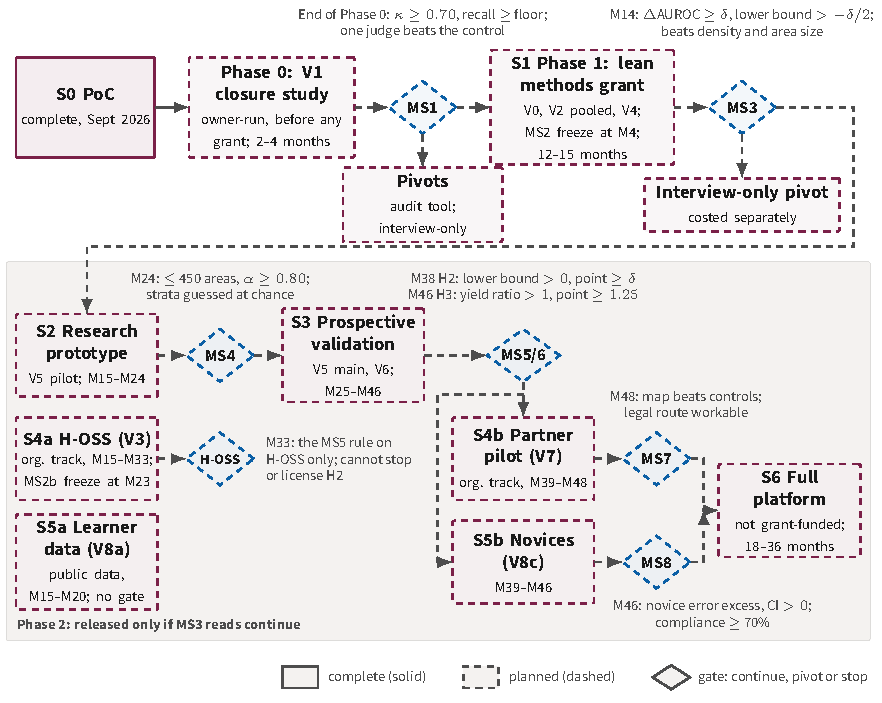
\includegraphics{figures/pdf/fig14_roadmap.pdf}
  \caption[Gated roadmap]{The roadmap in three phases, with the gate that releases each one.
  Phase~0 (owner-run, before any grant) is the closure study V1; it ends at MS1. Phase~1, a lean
  methods grant, starts only if MS1 reads continue and ends at the screening gate MS3. Phase~2
  starts only if MS3 reads continue; its prospective study decides H2 at MS5. The organizational
  track (H-OSS) runs inside Phase~2 and can neither stop nor license H2; the partner pilot waits
  for MS5.
  Every stop leads to a pivot with its own, smaller budget. Only S0 is complete.}
  \label{fig:roadmap}
\end{figure}

\begin{footnotesize}
\begin{longtable}{@{}>{\raggedright\arraybackslash}p{0.11\linewidth}>{\raggedright\arraybackslash}p{0.17\linewidth}>{\raggedright\arraybackslash}p{0.19\linewidth}>{\raggedright\arraybackslash}p{0.32\linewidth}>{\raggedright\arraybackslash}p{0.09\linewidth}@{}}
  \caption{The gated stages by phase: hypothesis tested, what gets built, the gate rule
    (continue / stop or pivot), and duration. S0 is complete; everything after it is future
    work. Months count from the start of Phase~1.}
  \label{tab:roadmap-stages}\\
  \toprule
  Stage & Hypothesis tested & What gets built & Gate: continue / stop or pivot & Duration \\
  \midrule
  \endfirsthead
  \toprule
  Stage & Hypothesis tested & What gets built & Gate: continue / stop or pivot & Duration \\
  \midrule
  \endhead
  \bottomrule
  \endfoot
  \textbf{S0 -- PoC} \evobs{} (complete) &
    H1 partly (reconstruction with provenance is feasible); H2 mechanism only &
    \code{residual/}, \code{reconstruct/}, \code{gapmap/}; three gap maps (PLC, GDPR v1, GDPR v2) &
    Closed. Engineering is complete. N2 reads inconclusive. N3 reads \enquote{pipeline complete,
      hidden-knowledge prediction not demonstrated} (\cref{sec:n2,sec:n3}) &
    Done \\
  \textbf{Phase~0 -- Closure study} (V1), owner-run, before any grant &
    L1: the absence check can be judged reliably, and retrieval finds a stating sentence where
      one exists &
    A closure codebook with anchors per lens; at least 100 double-coded units; a corpus-level
      retrieval-recall check; a judge panel scored against the fair control &
    \textbf{MS1 (closure verdict).} Continue if human $\kappa\geq0.70$, retrieval recall meets
      its floor, and one judge beats the fair control by the margin. Then write the Phase~1
      proposal with these numbers on page~1. Otherwise stop the automated absence check and take
      a pivot (\cref{sec:risks}) &
    2--4 mo \\
  \textbf{Phase~1 -- S1 Lean methods grant} (V0, V2 pooled, V4) &
    L0: trustworthy inputs. L2 (screening): the map beats the strongest baseline and adds value
      over density and area size on retrospective gold. L3: the residual is measurable &
    The area score; dated-corpus mode; the MS2 freeze at about M4 (the judge from MS1, then
      lexicons, thresholds, judge and area score hash-frozen, then gold acquired); the judge
      checked on each dated reconstruction's text &
    \textbf{MS3 (screening gate, not a verdict on H2).} Release Phase~2 only if the pooled
      $\Delta$AUROC point estimate is $\geq\delta$, its lower 90\% bound is $>-\delta/2$, and
      the map adds value over density and area size. Otherwise stop H2 funding and take the
      interview-only pivot. There is no inconclusive route &
    12--15 mo; MS3 at about M14 \\
  \textbf{Phase~2 -- S2 Research prototype} (V5 pilot) &
    Blind prospective elicitation is feasible at the powered size &
    An elicitation workbench: question service, blind-arm separation, World C records, coding
      tools, residual accounting. Track A components reused by copy, never import &
    \textbf{MS4.} Release V5's main study only if the pilot's projected number of areas fits
      the funded ceiling of 450, segmentation reaches $\alpha\geq0.80$, and stratum guessing
      stays near chance. Otherwise stop before the main study; H2 is reported as untested, and no
      underpowered V5 is run &
    M15--M24 \\
  \textbf{S3 -- Prospective validation} (V5 main, V6) &
    L4: predictions hold on fresh blind elicitation in held-out domains; this decides H2. H3:
      targeted questions yield more validated items per expert hour &
    The workbench for two held-out domains; leave-one-domain-out runs; expected information gain
      (EIG) question selection (future work N6) &
    \textbf{MS5 (H2 verdict).} Stop if the upper 90\% bound of $\Delta$AUROC is $<\delta$.
      Continue if the lower bound is $>0$ and the point estimate is $\geq\delta$. Anything else is
      reported as not supporting H2 and ends H2 funding. \textbf{MS6 (H3).} Continue if the
      yield-ratio lower bound is $>1$ and the point estimate is $\geq1.25$; any other reading
      counts against H3 &
    M25--M46 \\
  \textbf{S4 -- Organizational track} (V3, V7) &
    H-OSS: the gap map, adapted to code and commit evidence, predicts where knowledge is lost
      when developers leave. L5b: transfer to one partner &
    A World B Git adapter and code lenses, frozen at MS2b once the adapter exists; for V7, one
      tenant's ingestion, an on-prem judge stack, pseudonymization and an audit trail &
    \textbf{H-OSS gate.} The MS5 rule, on a clustered $\Delta$AUROC; it can neither stop nor
      license H2. \textbf{MS7 (V7).} Runs only after MS5 reads continue; the map beats density
      and random controls in both parts, and the legal route is workable &
    H-OSS M15--M33; V7 M39--M48 \\
  \textbf{S5 -- Education pilot} (V8a, V8c, materials) &
    L5c: confirmed residual areas carry more novice errors; teaching validated residual items
      changes a delayed outcome &
    Materials built \emph{only} from criterion-labeled, validated items (\cref{sec:platform}); a
      novice task set; manipulation-check logging &
    \textbf{MS8.} Continue if the error-excess interval lies above 0 and compliance is
      $\geq70\%$. No excess: expert residual and learner difficulty are different constructs, and
      no learner-facing feature uses the residual score. V8c starts only after MS5 reads continue &
    V8a M15--M20; V8c M39--M46 \\
  \textbf{S6 -- Full platform} (not grant-funded) &
    Commercial: residual accounting per knowledge unit is usable, legal, and worth paying for &
    A multi-tenant platform, connectors, compliance defaults in the core, a residual corpus with
    tenant isolation &
    Continue if at least two partners renew or pay and legal review is clean. MS5 not continue:
      no platform is built on the H2 claim. MS7's legal block recurs with a second partner: no
      organizational product &
    18--36 mo after S3 and S4 \\
\end{longtable}
\end{footnotesize}

\subsection{Parallel streams and where the money stops}

Phase~0 runs alone. It needs no grant, no participants and no new software, only one blind
second coder and local compute. Phase~1 runs its work in one line: build the area score and dated-corpus mode,
freeze at MS2, reconstruct, check the judge on the new text, then acquire gold and read MS3. Nothing in Phase~1 builds the
workbench, the Git adapter or any Phase~2 component, so no Phase~2 spending runs ahead of MS3.

Phase~2 has three streams. The prospective stream (S2, S3) waits for MS3, and V5's main study
waits for MS4. The organizational track (S4) starts with Phase~2, freezes its code lenses at MS2b
and reads H-OSS at its own gate. H-OSS cannot kill or license H2, and H2's gates do not read V3.
The partner pilot (V7) starts only after MS5 reads continue. The education stream runs V8a on public data early and V8c only after MS5. Validation
Track A runs on its own registered preconditions at any time; no gate here schedules or blocks it
(\cref{sec:validation}).

\begin{keyquestionbox}
  \textbf{Where the money stops.} Each phase is released by one gate, read by the external gate
  reader against the pre-registration.
  \begin{itemize}[noitemsep]
    \item \textbf{MS1 stops:} no grant is requested for the gap map. The ledger continues as a
      documentation-audit tool, or the interview-only pivot is proposed on its own budget.
    \item \textbf{MS3 does not release Phase~2:} H2 funding ends. The interview-only pivot tests
      targeted interviewing guided by expected information gain, without any reconstruction
      prior, on its own smaller budget (\cref{sec:resources}).
    \item \textbf{MS5 does not read continue:} H2 is reported as not supported, and no money is
      released for V6, V7, V8c or a platform built on the H2 claim. The interview-only pivot
      remains open on its own budget.
  \end{itemize}
  MS3 is a screening gate: it decides whether Phase~2 money is worth releasing. Only MS5 decides
  H2 as defined. No later stage can undo what either gate decides.
\end{keyquestionbox}

\section{Work packages}
\label{sec:workpackages}

This section is future work \evfut{} throughout. WP1--WP11 derive from the phased roadmap in
\cref{sec:roadmap} and from the validation program's studies V0--V8 (\cref{sec:validation}).
Months count from the start of Phase~1 (M1). Phase~0 comes before M1 and before any grant; it is
owner-run and marked P0. Phase~1 runs M1--M14 and ends at MS3. Phase~2 runs M15--M48 and starts
only if MS3 reads continue; if Phase~2 is a separate award, its months shift by the funder's
review time.

\Cref{fig:gantt} gives the schedule and dependencies as one diagram. \Cref{tab:milestones} gives
the gates. Each work package below gives its phase, objective, key tasks, deliverables, milestones
and main risks. Person-months per phase are in \cref{sec:resources}; roles are in \cref{sec:team}.

\begin{figure}[tbp]
  \centering
  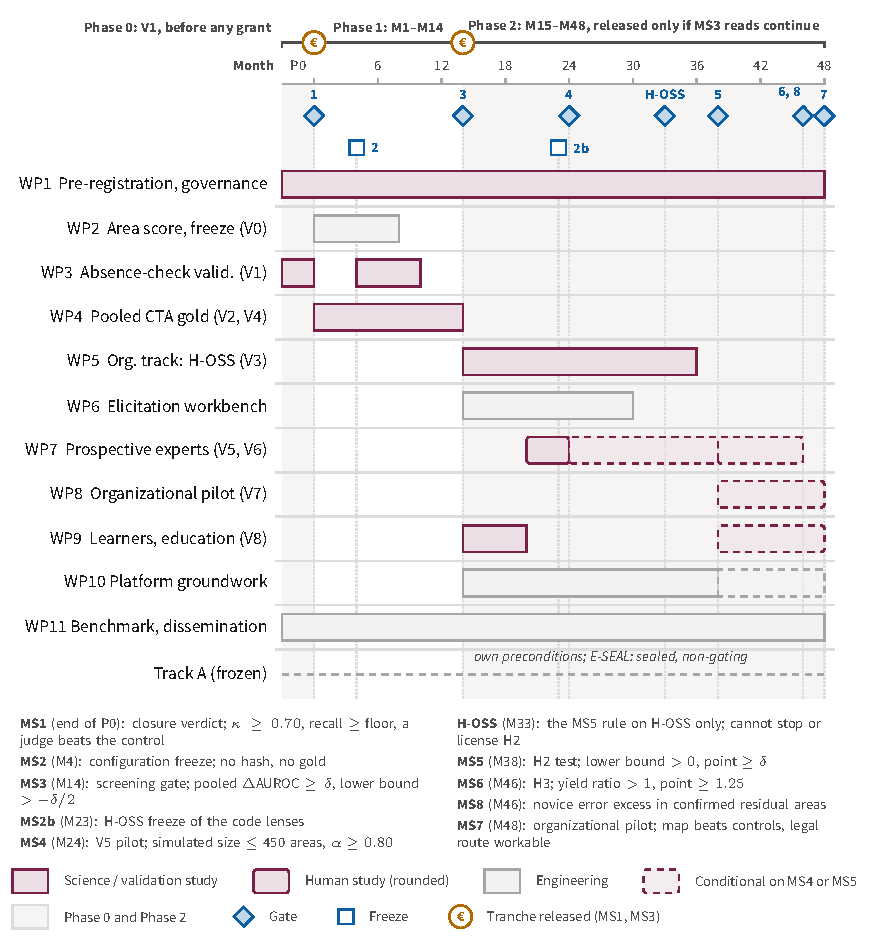
\includegraphics{figures/pdf/fig15_gantt.pdf}
  \caption[Work package schedule]{Work packages by phase, with gates as diamonds, the MS2 and MS2b
  freezes as squares, and the tranche releases at MS1 and MS3 as coins. Phase~0 (before
  M1, owner-run) ends at MS1, the closure verdict. Phase~1 (M1--M14) builds the area score,
  freezes the configuration at MS2 (about M4), and only then acquires gold; it ends at MS3
  (about M14). Phase~2 bars (M15--M48) are
  released only if MS3 reads continue. Inside Phase~2, V5's main study waits for MS4, and V6, V7
  and V8c wait for MS5. The organizational track freezes its code lenses at MS2b and reads H-OSS
  at its own gate. Validation Track A runs on its own preconditions and is not scheduled by this
  chart.}
  \label{fig:gantt}
\end{figure}

\footnotesize

\paragraph{WP1 -- Pre-registration, governance and data protection (P0, Phases 1--2)}
\mbox{}\par
\begin{tabularx}{\linewidth}{@{}>{\bfseries}p{2.6cm}X@{}}
  \toprule
  Objective & Every gate is fixed before its data exist, an independent reader checks it, and
    every human-data step is legal. \\
  Key tasks & P0: hash-commit the V1 pre-registration (codebook, $\kappa$ floor, retrieval-recall
    floor, judge margin, analysis script) before coding; appoint the external gate reader before
    MS1 is read. Phase~1: fill the threshold table ($\delta = 0.05$ recommended,
    \cref{sec:validation}); pre-register V0, V2 and V4, including V2's pooled and incremental
    analysis and the list of eligible golds; license checks; the budget headroom rule
    (\cref{sec:resources}); per-domain eligibility registers. Phase~2: ethics for V5, V6 and V8c,
    submitted at M15; V5 pre-registered at the powered size (M24); H-OSS (M23) and V6 (M38)
    pre-registrations; DPIA and works-council preparation for V7 after MS5. \\
  Deliverables & V1 pre-registration (P0); threshold table and V0/V2/V4 pre-registrations (M4);
    ethics approval for V5/V6 (M19); V5 pre-registration (M24); DPIA and data agreement for V7
    (M42); final data-management and open-data report (M48). \\
  Milestones & MS2 (M4, shared with WP2). \\
  Main risks & Thresholds set after data are seen; ethics delay pushes V5; legal cost of V7. \\
  \bottomrule
\end{tabularx}

\paragraph{WP2 -- Area score, configuration freeze and deferred N2 validation (V0; Phase~1)}
\mbox{}\par
\begin{tabularx}{\linewidth}{@{}>{\bfseries}p{2.6cm}X@{}}
  \toprule
  Objective & Make pipeline outputs admissible as inputs to a gold test (L0), and give the gap map
    an area-level score, which the PoC does not produce. \\
  Key tasks & Build a pre-registered area score from the \emph{uncapped} candidate set within an
    area (for example max or noisy-OR over candidate scores), chosen on PLC and GDPR pilot data
    only. Check that it is not a monotone function of area size or source density, and report its
    partial correlation with density. Add an \code{--areas} input at task-step grain. Build
    admissibility checks as code. Build dated-corpus mode (its source and date rule are in
    \cref{sec:validation}) with a gold blocklist, and count the dated sources each candidate gold
    reaches. Run the deferred N2 protocols as registered (E-LIVE v3, E-PLANT run 2, E-ABST run
    2). Then freeze: the judge chosen at MS1, lexicons, thresholds, the area score and the list of
    eligible golds are hash-committed together at MS2. Depends on MS1 and WP1. \\
  Deliverables & Area score, admissibility checker and dated-corpus source pilot (M3); frozen
    configuration hash (M4); N2 deferred-validation report (M8). \\
  Milestones & MS2 (M4): no hash, no gold. \\
  Main risks & Live runs expose new defects, as they did in N2; dated corpora too small for a
    gold domain; the area score tracks density. \\
  \bottomrule
\end{tabularx}

\paragraph{WP3 -- Absence-check validation (V1 in P0; judge text-type check in Phase~1)}
\mbox{}\par
\begin{tabularx}{\linewidth}{@{}>{\bfseries}p{2.6cm}X@{}}
  \toprule
  Objective & Decide whether \enquote{is this element really unsaid?} can be judged reliably,
    by humans and by a judge, and whether retrieval finds the element where it is stated (L1). \\
  Key tasks & P0 (owner-run): write a closure codebook with anchors per lens. Code the 107
    admissible lens firings in both arms of the fair control, plus about 100 units from one new
    non-gold domain; the owner (under origin blinding) and one non-owner coder code every unit.
    Report weighted human--human $\kappa$ on three states, gated on closed versus not closed. For
    about 50 firings, search the ledger's full snapshots for the missing element and report
    retrieval recall. Score a judge panel (the local 7B model, a stronger open-weight judge, and
    frontier judges from other families) against the fair control. Phase~1: before any gold is
    unsealed, double-code a closure sample from each dated V2 reconstruction, to check the MS1
    judge on that text type; where it fails, closure there is human-coded. \\
  Deliverables & Codebook and V1 pre-registration (P0); closure set, released, and closure verdict
    report (end of P0); judge text-type report (M10). \\
  Milestones & MS1 (end of P0): the closure verdict. \\
  Main risks & Human--human $\kappa$ below 0.70 (the construct itself is unreliable); low
    retrieval recall; the judge overfits the codebook; the judge fails on the new text type. \\
  \bottomrule
\end{tabularx}

\paragraph{WP4 -- Pooled retrospective CTA gold test and residual check (V2, V4; Phase~1)}
\mbox{}\par
\begin{tabularx}{\linewidth}{@{}>{\bfseries}p{2.6cm}X@{}}
  \toprule
  Objective & Screen H2 on several published CTA golds before any expert is recruited (L2), and
    test whether the residual can be measured at all (L3). \\
  Key tasks & Check itemized gold availability by metadata and author contact only; the list of
    eligible golds (at least three proposed) is fixed at MS2. Build area partitions from dated
    pre-gold sources. After MS2, reconstruct on each dated corpus, then acquire each gold,
    sealed. Run per-item memorization
    probes and exclude probe-positive items. Map gold items to areas by blind double coding. Pool
    $\Delta$AUROC across golds by random effects, against the strongest baseline chosen inside
    each bootstrap resample. Test the map's incremental value over density and area size. Run the
    V4 known-truth check on V2 data. \\
  Deliverables & Gold availability report (M3); dated-corpus reconstructions (M10); pooled V2
    result and V4 report (M13); a public reconstruct-vs-CTA benchmark release (M16). \\
  Milestones & MS3 (M14). \\
  Main risks & Fewer than three eligible golds; contamination; unmappable gold items; wide pooled
    intervals. \\
  \bottomrule
\end{tabularx}

\begin{keyquestionbox}
  \textbf{MS3, about M14 -- the screening gate for Phase~2 money.} The external gate reader reads
  the pooled V2 result against the pre-registration. Phase~2 is released only if the point
  estimate is at least $\delta$, the lower 90\% bound is above $-\delta/2$, and the map adds value
  over density and area size. Otherwise H2 funding stops, no Phase~2 work package starts, and the
  interview-only pivot is proposed on its own budget. MS3 does not decide H2; MS5 does.
\end{keyquestionbox}

\paragraph{WP5 -- Organizational track: developer-departure study (V3, H-OSS; Phase~2)}
\mbox{}\par
\begin{tabularx}{\linewidth}{@{}>{\bfseries}p{2.6cm}X@{}}
  \toprule
  Objective & Test H-OSS: the gap map, adapted to code and commit evidence, predicts where
    knowledge is lost when developers leave. H-OSS is a separate hypothesis; it cannot kill or
    license H2. \\
  Key tasks & Build a World B Git adapter (commits, blame at time $t$, issues, pull requests,
    reviews, dated documentation) for public repositories. Develop code lenses on repositories
    outside the departure sample, and freeze them at MS2b (M23), after the adapter exists. Validate the
    closure judge on commit and issue text, or register V3 without closure. Pilot five departures
    to estimate the base rate, clustering and coding time; decide power. Run the main study if
    feasible, else register it as descriptive. Blind double code rationale-seeking issues and
    defect-fix commits; use a staggered-adoption difference-in-differences estimator
    \evlit{} \parencite{callaway2021difference}. Depends on WP1 (pseudonymization record). \\
  Deliverables & Git adapter with provenance (M22); code-lens freeze (M23); pilot and power
    decision (M26); H-OSS result (M33); coded post-departure dataset, pseudonymized (M36). \\
  Milestones & MS2b (M23); the H-OSS gate (M33), which uses the MS5 rule on H-OSS only. \\
  Main risks & Too few departures with enough later activity; authorship metrics may break under
    agentic coding; target repositories sit in model pretraining data. \\
  \bottomrule
\end{tabularx}

\paragraph{WP6 -- Elicitation workbench (research prototype; Phase~2)}
\mbox{}\par
\begin{tabularx}{\linewidth}{@{}>{\bfseries}p{2.6cm}X@{}}
  \toprule
  Objective & Build the minimum software that V5 and V6 need to run blind, logged, and codable. \\
  Key tasks & A question service (template questions now; expected-information-gain selection
    later, future work N6) with a fixed unknown-unknowns fraction; blind-arm separation, so the
    interviewer view never shows scores or strata; World C records into the ledger; a segmentation
    and coding tool with blinding checks; residual accounting and cost per validated item. The
    Track A turn contract, leading-question guard and corroboration code are copied into the new
    package; \code{instrument/} is never imported. Starts at M15, after MS3. \\
  Deliverables & Workbench v1, tested on simulated labeled sessions (M21); v2 for two domains
    (M30). \\
  Milestones & MS4 (M24) is the first gate to use it. \\
  Main risks & Leakage of scores or strata into the interviewer or coder views. \\
  \bottomrule
\end{tabularx}

\paragraph{WP7 -- Prospective expert validation (V5, V6; Phase~2)}
\mbox{}\par
\begin{tabularx}{\linewidth}{@{}>{\bfseries}p{2.6cm}X@{}}
  \toprule
  Objective & Decide H2 on fresh, blind human elicitation (L4), and test H3, whether targeting
    saves expert time (L5a). \\
  Key tasks & V5 pilot: 6 experts
    $\times$ 20 areas in PLC (40 areas, three experts each), not analyzed for effect; it measures
    prevalence, design effect, coding time and leakage (M21--M24). V5 main (M25--M37), sized for
    $\delta = 0.05$: about 300 areas (about 150 per class) in two held-out subdomains (D3, D4),
    strata G/D/L/R, and short neutral CDM probes of about 8 minutes
    \evlit{} \parencite{klein1989critical}. Each area is probed by 3 experts
    \evlit{} \parencite{chao1994percentage}, and each expert covers about 20 areas, so about 45
    experts are needed. V6 (M39--M45), only after MS5 reads continue: a
    targeted-versus-untargeted crossover with question-seeded coding against leading questions
    \evlit{} \parencite{loftus1975leading}. \\
  Deliverables & V5 pilot report and powered sample (M24); V5 main result
    (M38); V6 result (M46); residual corpus v1 (M46). \\
  Milestones & MS4 (M24); MS5 (M38), the H2 verdict; MS6 (M46), the H3 verdict. \\
  Main risks & Recruiting about 45 experts; a prevalence below one half, which raises the areas
    needed above MS4's funded ceiling; coding time; interviewer effects. \\
  \bottomrule
\end{tabularx}

\paragraph{WP8 -- Organizational pilot (V7; Phase~2)}
\mbox{}\par
\begin{tabularx}{\linewidth}{@{}>{\bfseries}p{2.6cm}X@{}}
  \toprule
  Objective & Test transfer to one partner organization (L5b) and whether the legal route is
    workable. \\
  Key tasks & Select a partner (a software organization first); complete a DPIA and a
    legitimate-interest balancing test; secure a works agreement where German co-determination
    applies; agree a data contract (no training on partner data; on-prem or equivalent hosting).
    Run the retrospective part (past departures or onboarding tickets as the outcome; the H-OSS
    design, if H-OSS has run) and the prospective part (the V5 design, on one or two critical
    units). Starts only after MS5 reads continue and the deferred N2 validation is complete.
    Depends on WP10's on-prem stack and WP1's legal groundwork. \\
  Deliverables & Signed partner and data agreements (M42); retrospective result (M45);
    prospective result and feasibility report (M48). \\
  Milestones & MS7 (M48). \\
  Main risks & Partner access; a works-council veto; staff reading the tool as surveillance;
    prompt injection through internal documents \evlit{} \parencite{greshake2023not}. \\
  \bottomrule
\end{tabularx}

\paragraph{WP9 -- Learner link and education pilot (N4, V8a, V8c, E-SEAL; Phase~2)}
\mbox{}\par
\begin{tabularx}{\linewidth}{@{}>{\bfseries}p{2.6cm}X@{}}
  \toprule
  Objective & Test whether the expert residual relates to learner difficulty, and whether
    teaching validated residual items changes anything measurable. \\
  Key tasks & (a) V8a on public mathematics data, after license checks (M15--M20). (b) An E-SEAL
    interface to Track A: sealed gap-map scores, added only if the Track A owner approves before
    Stage A. (c) V8c: 30--60 novices in a validated V5 domain, after a 10-novice pilot; it starts
    only after MS5 reads continue (M39--M45). (d) An education materials pilot built only from
    validated items, run as a manipulation check on one course section or apprentice cohort, not
    as a powered RCT (M45--M48). \\
  Deliverables & V8a report (M20); V8c result (M46); education pilot feasibility report and an
    RCT pre-registration draft (M48). \\
  Milestones & MS8 (M46). \\
  Main risks & Non-commercial data licenses; a null learner link, which is plausible and
    informative; learner data protection. \\
  \bottomrule
\end{tabularx}

\paragraph{WP10 -- Platform groundwork and World B infrastructure (Phase~2)}
\mbox{}\par
\begin{tabularx}{\linewidth}{@{}>{\bfseries}p{2.6cm}X@{}}
  \toprule
  Objective & Turn the PoC's properties into the platform's core, without building features ahead
    of evidence. \\
  Key tasks & A typed run-status record, replacing the untyped sidecar; ledger storage that scales
    beyond one JSON file per run, which V5's volume needs. After MS5 reads continue: an on-prem
    stack spanning three model families (generator, verifier, closure judge); access-control
    propagation to labels (a claim inherits its evidence's most restrictive access control); an
    erasure design (pseudonym key kept outside the ledger); a hash-chained audit trail. \\
  Deliverables & Typed run status and scalable ledger (M24); on-prem judge stack (M43); access
    control, erasure and audit for the WP8 tenant (M46); a platform decision record for S6,
    written only if MS5 and MS7 read continue (M48). \\
  Milestones & Supports MS7. \\
  Main risks & Building for customers before MS5 reads; on-prem judges weaker than hosted ones. \\
  \bottomrule
\end{tabularx}

\paragraph{WP11 -- Open benchmark, residual corpus and dissemination (all phases)}
\mbox{}\par
\begin{tabularx}{\linewidth}{@{}>{\bfseries}p{2.6cm}X@{}}
  \toprule
  Objective & Make the program's outputs reusable whatever the gates read. \\
  Key tasks & Release the closure set, the reconstruct-vs-CTA benchmark, the coded post-departure
    dataset, a consented subset of the residual corpus, and every pre-registration and negative
    result. Publish a paper after each gate. Licenses and consent are cleared by WP1. \\
  Deliverables & Releases at the end of P0 (closure set), M16, M36, M46 and M48; papers after MS1,
    MS3, MS5, MS6, MS7 and the H-OSS gate. \\
  Milestones & Tied to the releases above. \\
  Main risks & Gold licenses that forbid redistribution; mitigated by releasing mappings and code,
    never the gold text itself. \\
  \bottomrule
\end{tabularx}

\normalsize

\FloatBarrier
\subsection{Milestones}

\Cref{tab:milestones} lists every gate in time order, with its phase, its month and the rule that
reads it. The external gate reader reads MS1, MS3 and MS5, and signs off any owner exception
at any gate (\cref{sec:team}).

\begin{table}[!htbp]
  \centering
  \small
  \caption{Milestones in time order: phase, month, and the rule that reads each gate. MS1
  releases Phase~1, MS3 releases Phase~2, and MS5 decides H2. MS2 and MS2b are freezes: no hash,
  no data.}
  \label{tab:milestones}
  \begin{tabularx}{\linewidth}{@{}lllX@{}}
    \toprule
    Milestone & Phase & Month & Gate rule \\
    \midrule
    MS1 & 0 & P0 end & \textbf{Closure verdict.} Continue if human $\kappa\geq0.70$, recall meets
      its floor, and one judge beats the fair control by the margin; this releases the Phase~1
      proposal. Otherwise stop the automated absence check and take a pivot. \\
    MS2 & 1 & M4 & Configuration freeze: MS1's judge, lexicons, thresholds, area score, the V0,
      V2 and V4 pre-registrations and the list of eligible golds hash-committed. No gold before
      it. \\
    MS3 & 1 & M14 & \textbf{Screening gate.} Release Phase~2 only if the pooled $\Delta$AUROC point
      estimate is $\geq\delta$, its lower 90\% bound is $>-\delta/2$, and the map adds value over
      density and area size. Otherwise stop H2 funding. \\
    MS2b & 2 & M23 & H-OSS freeze: code lenses and the H-OSS pre-registration hash-committed, after
      the Git adapter exists. \\
    MS4 & 2 & M24 & V5 pilot: the projected number of areas fits the funded ceiling of 450,
      segmentation $\alpha\geq0.80$, and stratum guessing stays near chance. \\
    H-OSS & 2 & M33 & The MS5 rule, applied to H-OSS only; it can neither stop nor license H2. \\
    MS5 & 2 & M38 & \textbf{H2 verdict.} Stop if the upper 90\% bound $<\delta$; continue if the
      lower bound $>0$ and the point estimate $\geq\delta$; otherwise not supporting H2, and H2
      funding ends. \\
    MS6 & 2 & M46 & H3: yield-ratio lower bound $>1$ and point estimate $\geq1.25$ (the smallest
      effect size of interest, SESOI); any other reading counts against H3. \\
    MS8 & 2 & M46 & Novice error excess in confirmed residual areas. \\
    MS7 & 2 & M48 & Organizational pilot: the map beats density and random controls in both parts;
      the legal route is workable. \\
    \bottomrule
  \end{tabularx}
\end{table}
\FloatBarrier

\section{Team and competencies}
\label{sec:team}

\begin{evfutbox}
  No team exists yet. There is no host institution, no named principal investigator (PI) record
  for this program, no statistician, no CTA collaborator, no gate reader and no letter of support.
  The configurations below are planning constructs, sized from the PoC's own operating experience
  and from the work-package plan in \cref{sec:workpackages}. Every full-time-equivalent (FTE) figure is an indicative
  range, not a hire request.
\end{evfutbox}

\subsection{Team status today}

The PoC was designed, built, run and read by a single operator with AI assistance
(\cref{sec:threats-ai}). The same person was its only coder and is the prospective applicant; the
single-operator threat is rated in \cref{sec:threats}. This report names no other person and
claims no commitment from anyone. The following must be named, with written commitments, before
the step shown:

\begin{itemize}[noitemsep]
  \item \textbf{Before MS1 is read (Phase~0):} the non-owner blind coder, and the external gate
    reader.
  \item \textbf{Before the Phase~1 proposal is submitted:} the host institution and its
    person-month rate; the PI and the PI's record; a statistician as co-applicant; a CTA
    collaborator who can help locate itemized golds; a research engineer; a data-protection and
    license advisor.
  \item \textbf{Before Phase~2 is released:} a cognitive psychologist or CTA lead for V5; expert
    pools for the two held-out domains, with letters from professional bodies; a learning
    scientist.
  \item \textbf{Before V7 is scheduled (after MS5):} a partner's letter of intent.
\end{itemize}

\subsection{Why the program is interdisciplinary}

Each hard problem in the program belongs to a different research tradition, and no single skill
covers all of them.

\begin{itemize}[noitemsep]
  \item \textbf{The absence check} is a natural-language-processing and measurement problem
    (\cref{sec:n3,sec:resources}).
  \item \textbf{Eliciting a fair question from a predicted gap} is a cognitive-task-analysis
    problem, not a prompting technique (\cref{sec:foundations}).
  \item \textbf{Matching a predicted gap to what a novice finds hard} is a learning-science
    problem, because expert and instructor judgment of learner difficulty is unreliable
    (\cref{sec:education-blindspots}).
  \item \textbf{Deciding whether an effect is real at a pre-set size} is a statistics problem
    (\cref{sec:validation}).
  \item \textbf{Deploying on an organization's documents} is a security, privacy and legal problem
    (\cref{sec:organizations}).
\end{itemize}

\evint{} A team of machine-learning engineers alone cannot cover this list, and a team of domain
researchers alone cannot build the pipeline. The configurations below follow this map.

\subsection{Configurations by phase}

The team grows only when a gate releases the next phase.

\paragraph{Phase~0 (owner-run, no hires).} The owner prepares the units and the codebook. One
non-owner blind coder codes on an hourly contract, and the owner codes only under reported origin
blinding. The external gate reader reads MS1. Nothing else is needed.

\paragraph{Phase~1 lean team.} This is the minimum team that removes the PoC's largest structural
risk, one person who built, ran, coded and read everything, and that can reach MS3
(\cref{tab:team-lean}). It funds the area score and freeze (WP2), the judge's text-type check
(WP3), and the pooled retrospective study (WP4). The Git adapter and V3 are no longer in this
phase.

\begin{table}[htbp]
  \centering
  \footnotesize
  \caption{Phase~1 lean team (12--15 months, about 2.5--3.0~FTE, 35--44 person-months). It
    reaches the screening gate MS3.}
  \label{tab:team-lean}
  \begin{tabularx}{\linewidth}{@{}p{0.19\linewidth}Xp{0.13\linewidth}p{0.07\linewidth}p{0.12\linewidth}@{}}
    \toprule
    Role & Why needed & When (WP) & FTE & Permanent / consultant \\
    \midrule
    PI / research lead &
      Owns hypotheses and thresholds; prepares each gate report, but does not read the gate &
      WP1, all & 0.8--1.0 & Permanent \\
    Research engineer (LLM/retrieval) &
      Area score, admissibility as code, dated-corpus mode, the freeze, V0 &
      WP2, WP4 & 1.0 & Permanent \\
    Research assistant or second engineer &
      Gold availability check, area partitions, memorization probes &
      WP4 & 0.5 & Fixed-term \\
    Statistician / methodologist &
      Threshold table, pooled random-effects $\Delta$AUROC, incremental analysis; script
      committed before any gold is seen &
      WP1, WP3, WP4 & 0.3 & Part-time \\
    CTA practitioner &
      Codebook upkeep; rules for mapping gold items to areas &
      WP3, WP4 & 0.1--0.2 & Consultant \\
    Coders (2) &
      Judge text-type units; blind gold-to-area mapping &
      WP3, WP4 & 160--380 hours & Hourly contract \\
    Data-protection / license advisor &
      Dataset and gold license checks &
      WP1, ad hoc & Ad hoc & Consultant \\
    External gate reader &
      Reads MS3; not a team member (\cref{sec:gate-reader}) &
      MS3 & Per gate & Independent \\
    \bottomrule
  \end{tabularx}
\end{table}

\paragraph{Phase~2 team.} \evint{} This is the smallest team that can run Phase~2 without leaving
any stage's human-science, statistics or engineering skill missing when it starts
(\cref{tab:team-grant}). It adds a cognitive psychologist, a platform engineer, a learning
scientist, human--computer interaction (HCI) support, and the legal and project-management capacity V7 needs. Without the
organizational track, the platform engineer and legal counsel lines can be dropped. The role
table is in \cref{app:program}, since it matters only once MS3 reads continue.


\paragraph{Product / platform team.} \evfut{} This configuration starts only after MS5 and MS7
both read continue (\cref{sec:workpackages}). A research grant does not fund it; it is sized only
for comparison with the research teams above, at close to the \enquote{team of 8--15} used in
\cref{sec:resources}. The role table is \cref{tab:team-product} in \cref{app:program}.

\subsection{The external gate reader}
\label{sec:gate-reader}

\evint{} A funder buying pre-registered kill criteria needs someone other than the applicant to
apply them. The program therefore names an external gate reader: an independent statistician, or
a small advisory board that includes one.

\begin{itemize}[noitemsep]
  \item \textbf{Independence.} The reader is not a co-applicant, is not paid from a tranche that
    the reading releases, and has no stake in the program's continuation. A per-gate fee is agreed
    in advance.
  \item \textbf{Authority.} The reader reads MS1, MS3 and MS5 against the pre-registration,
    which is hash-committed in advance. The reading is binding: a tranche is released only if the reader reads
    continue.
  \item \textbf{Owner exceptions.} Any exception the owner wants at any gate, including MS2, MS2b,
    MS4, MS6, MS7, MS8 and the H-OSS gate, needs the reader's written sign-off before it takes effect. An exception
    without sign-off voids the gate reading, and no money is released on it.
\end{itemize}

No such reader existed during the PoC. The step from N2 to N3 was an owner exception, recorded
but not checked by anyone independent (\cref{sec:evolution}). The gate reader exists so that this
cannot recur.

\subsection{The independence rule (binding for staffing)}

One rule constrains every configuration above and cannot be relaxed by adding headcount. A domain
expert who serves as a study participant cannot also be an advisor who has seen the
reconstruction or its candidates for that domain. The same rule already governs the frozen
Validation Track~A. There, anyone who has seen reconstructed conservation content is ineligible
for any Track~A human role: interviewer, corroborating coder, K1 \enquote{absent} coder, or
importance rater (\emph{REORIENTATION.md} \S18.1). The NOW program extends the same logic to every
new domain:

\begin{itemize}[noitemsep]
  \item \textbf{Advisor versus participant.} An advisor who saw a domain's gap map or candidates
    may not later rate, be interviewed, code, or corroborate in that domain (eligibility register,
    WP1).
  \item \textbf{The Track~A roster stays separate.} Mechanics-domain staff are excluded from any
    Track~A role; E-SEAL predictions are script-generated, never shown to a future Track~A holder.
  \item \textbf{The pipeline's owner cannot be the blind coder.} Every gating agreement score includes a
    non-owner coder; the owner may code only under reported origin blinding, as in Phase~0.
  \item \textbf{Interviewers and coders never see scores or strata.} A guess-the-stratum check on a
    fifth of V5's areas measures whether this blinding held.
\end{itemize}

\evint{} These rules cost recruiting effort. Each domain needs at least one advisor and a disjoint
pool of participants, so \cref{sec:resources} counts recruitment overhead as its own line.

\section{Resources and indicative timeline}
\label{sec:resources}

\begin{evfutbox}
  Every figure below is a planning range, not an estimate fitted to data: nothing in the
  validation program (\cref{sec:validation}) has run. Personnel cost per person-month (PM) varies
  by a factor of two or more across European countries and institution types. The range used
  here, EUR~6{,}000--10{,}000 per PM fully loaded, should be replaced with the host institution's
  own rate once a host is named (\cref{sec:team}).
\end{evfutbox}

\subsection{Money released by each gate}

The budget is split into tranches, and each tranche is released only when the gate before it
reads continue (\cref{sec:roadmap}). \Cref{tab:resources-totals} gives each tranche's gate, scope,
effort and cost. Phase~2 has two lines. The main line (2a--2c) carries H2, H3, the partner
pilot and the learner link; the organizational line (O) carries H-OSS. Phase~0 is owner-run and
needs no grant.

\begin{table}[htbp]
  \centering
  \footnotesize
  \caption{Tranches, the gate that releases each, and indicative cost. PM at EUR 6--10k; other
    direct costs are participants, coders, compute, legal, open access, travel and the gate
    reader's fee. Months count from the start of Phase~1.}
  \label{tab:resources-totals}
  \begin{tabularx}{\linewidth}{@{}>{\raggedright\arraybackslash}p{0.1\linewidth}>{\raggedright\arraybackslash}p{0.11\linewidth}>{\raggedright\arraybackslash}X>{\raggedright\arraybackslash}p{0.1\linewidth}p{0.07\linewidth}p{0.09\linewidth}p{0.11\linewidth}@{}}
    \toprule
    Tranche & Released by & Scope & Months & PM & Other direct & Total (EUR) \\
    \midrule
    Phase~0 & Owner, before any grant & V1 closure study (WP3) & 2--4 mo before M1 & Owner time &
      $\approx10^3$ & $\approx10^3$ \\
    Phase~1 & MS1 continue & Area score, freeze, V0, judge text-type check, pooled V2, V4 (WP1--4,
      WP11) & M1--M14 & 35--44 & 20k--70k & \textbf{0.23--0.51\,M} \\
    2a & MS3 continue & Workbench, V5 pilot, V8a, ledger groundwork & M15--M24 & 29--44 &
      15k--50k & 0.19--0.49\,M \\
    2b & MS4 continue & V5 main, powered; high end at the 450-area ceiling & M25--M38 & 22--36 &
      35k--250k & 0.17--0.61\,M \\
    2c & MS5 continue & V6, V7, V8c, education pilot, on-prem stack & M39--M48 & 38--62 &
      35k--165k & 0.26--0.79\,M \\
    O & MS3 continue & Git adapter, code lenses, V3 (H-OSS) & M15--M36 & 14--22 & 5k--35k &
      0.09--0.26\,M \\
    \midrule
    \textbf{Phase~2} & & 2a--2c and O & M15--M48 & 103--164 & 90k--500k &
      \textbf{0.7--2.2\,M} \\
    \textbf{Program} & & Phases~1 and 2 & 48~mo & 138--208 & 110k--570k & \textbf{0.9--2.7\,M} \\
    \midrule
    Interview-only pivot & MS1, MS3 or MS5 stop & Separate line (see below) & 18--24~mo & 21--31 &
      15k--70k & 0.14--0.38\,M \\
    Product (S6) & MS5 and MS7 & Team of 8--15 & 18--36~mo later & -- & Hosting, sales &
      Outside this estimate \\
    \bottomrule
  \end{tabularx}
\end{table}

\evint{} At EUR~8k per PM, Phase~1 costs EUR~0.30--0.42\,M; the full range is EUR~0.23--0.51\,M,
so about EUR~0.3--0.5\,M. Every Phase~2 euro waits for MS3.

\paragraph{Money at risk if H2 fails.} The spend on H2 before a failure is visible depends on the
gate that reads it.
\begin{itemize}[noitemsep]
  \item \textbf{At MS1:} about EUR~$10^3$ of coder time and compute, plus the owner's time.
  \item \textbf{At MS3:} Phase~1, EUR~0.23--0.51\,M. It still leaves a released closure set, a
    frozen area score and a public reconstruct-versus-CTA benchmark.
  \item \textbf{At MS4:} Phase~1 plus tranche 2a, EUR~0.42--1.00\,M.
  \item \textbf{At MS5:} Phase~1 plus 2a and 2b, EUR~0.59--1.61\,M. Tranche 2c, EUR~0.26--0.79\,M,
    is never released.
\end{itemize}
The organizational line is outside these sums because H-OSS does not depend on H2. It runs to its
own gate whatever H2's gates read, and it releases no partner pilot on its own.

\paragraph{The interview-only pivot, costed separately.} If MS1 stops the automated absence check,
or MS3 or MS5 ends H2 funding, the program can propose one smaller study. It tests targeted
interviewing guided by expected information gain against untargeted interviewing, with no
reconstruction prior. It needs a light workbench (8--12 PM), the efficiency study in
interview-only form (10--14 PM), ethics and pre-registration (2--3 PM), and release (1--2 PM).
Participants and coders add EUR~15k--70k. The line is a new proposal read by the gate reader; it never draws on Phase~2's
budget.

\subsection{Person-months per work package}

\Cref{tab:resources-pm} gives effort by work package and phase. Coder hours are counted under
participant costs (\cref{tab:resources-participants}), not here, because they are hourly
contracts. Phase~1's 35--44 PM over 12--15 months fit a team of 2.5--3.0~FTE; Phase~2's 103--164
PM over 34 months average 3.0--4.8~FTE (\cref{sec:team}). V5's main study concentrates about
22--36 PM in 14 months, which is why the CTA practitioner rises to full time in S3.

\begin{table}[htbp]
  \centering
  \footnotesize
  \caption{Person-months per work package and phase.}
  \label{tab:resources-pm}
  \begin{tabularx}{\linewidth}{@{}Xp{0.1\linewidth}p{0.1\linewidth}p{0.3\linewidth}@{}}
    \toprule
    Work package & Phase~1 & Phase~2 & Main roles \\
    \midrule
    WP1 Pre-registration, governance, data protection & 4--5 & 6--10 &
      PI, project manager, statistician, counsel \\
    WP2 Area score, freeze, deferred N2 validation (V0) & 10--13 & -- &
      Research engineer \\
    WP3 Absence-check validation (V1 in P0; text-type check) & 4--6 & -- &
      CTA practitioner, statistician, engineer \\
    WP4 Pooled CTA gold test and residual check (V2, V4) & 15--18 & -- &
      Engineer, research assistant, statistician \\
    WP5 Organizational track: H-OSS (V3) & -- & 14--22 &
      AI/ML researcher, platform engineer, statistician \\
    WP6 Elicitation workbench & -- & 16--25 &
      Software engineer, frontend/HCI, CTA practitioner \\
    WP7 Prospective expert validation (V5, V6) & -- & 31--49 &
      CTA practitioner, interviewers, statistician \\
    WP8 Organizational pilot (V7) & -- & 10--16 &
      Project manager, security, counsel, CTA practitioner \\
    WP9 Learner link and education pilot & -- & 10--16 &
      Learning scientist, statistician \\
    WP10 Platform groundwork & -- & 12--20 &
      Platform engineer, security engineer \\
    WP11 Open benchmark and dissemination & 2 & 4--6 &
      PI, research engineer \\
    \midrule
    \textbf{Total} & \textbf{35--44} & \textbf{103--164} & \\
    \bottomrule
  \end{tabularx}
\end{table}

\subsection{Compute, API budgets, and the headroom lesson}

\evobs{} The PoC gives one hard number to plan from: a single reconstruction run cost \$0.68 (PLC)
or \$0.50 (GDPR).\footnote{\repo{research/n2/e_plant_eabst_report.md} \S1.2, \S3;
\repo{research/n3/README.md}.} Money was not the constraint; \textbf{headroom} was. A weekly key
limit of \$5, set below the sum of the experiments' registered caps (about \$21), blocked E-LIVE~v3 at its first
call.\footnote{\repo{docs/lessons.md}.} The budget stop is one reason N2's gated arms were never
scored (\cref{sec:n2}).

\evint{} The lesson has four parts. (1)~Provider spending limits are set at least 3$\times$ the sum
of a stage's registered caps, on a monthly window, and recorded in the protocol before the first
run. (2)~The headroom check runs as code before a run sequence starts. (3)~Each experiment has its
own API key, so one study cannot exhaust another's budget. (4)~Every study reports cost per
\emph{validated} item, not cost per claim.

Later stages cost more per run than the PoC did. A decisive test needs at least three reruns per
task, because retrieval variance dominated the PoC's cross-run instability. It also needs two or
three model families for the generator, verifier and closure judge, stronger models, plain-LLM
baselines, memorization probes and, on the organizational line, repository histories.
Compute stays small next to personnel: about EUR~$10^3$--$10^4$ in Phase~1 and
EUR~$10^3$--$10^4$ per tranche in Phase~2. \Cref{tab:resources-compute} in \cref{app:program}
gives the orders of magnitude by phase.


\subsection{Participant, coder and expert-hour costs}

\Cref{tab:resources-participants} in \cref{app:program} gives honoraria or wages, not
consulting rates, at the volumes set by \cref{sec:validation}. Expert time is costed at EUR~60--200 per hour and coder time at
EUR~20--45 per hour. Over Phase~2, participant, coder and learner costs run roughly EUR~55k--355k,
the high end at V5's funded ceiling. Other direct costs (legal counsel, compute, open access,
travel, ethics fees, the gate reader) add roughly EUR~35k--140k.

\paragraph{V5 is budgeted for power.} \evint{} Deciding H2 at $\delta = 0.05$ needs about 300
areas, about 150 per class (\cref{sec:validation}). With 3 experts per area, that is about 900
probes of about 8 minutes each. At about 20 areas per expert, V5 needs about 45 experts, about 22
per domain, plus 6 in the pilot. Each expert gives about 3 hours in sessions and 1 hour rating
other experts' items: about 150--250 expert-hours in all, and about 70 session hours per
interviewer. Coding costs more than the experts: about 120 hours of audio need 1,200--1,900 coder
hours. Honoraria, recruitment and coding come to roughly EUR~40k--160k before staff time. MS4
releases the main study only if the pilot's projection fits a funded ceiling of 450 areas, so
tranche 2b's high end is costed at that ceiling. At a prevalence of 0.3, about 500 areas would be
needed; that exceeds the ceiling, and MS4 would not release V5. The binding constraint is
recruiting about 45 eligible experts, not money.


\subsection{Timeline uncertainty}

\evint{} Four facts drive most of the uncertainty, and none can be resolved before the program
starts:
\begin{itemize}[noitemsep]
  \item the number of itemized CTA golds that can be obtained and dated (fewer golds mean fewer
    areas, which makes CONTINUE at MS3 harder to reach);
  \item the prevalence of residual-present areas and the coding time per probe in V5 (they
    scale areas, expert-hours and coder hours);
  \item the number of usable developer departures for H-OSS;
  \item the host institution's rate, and whether V7's legal work takes weeks or months.
\end{itemize}
A stop at MS1, MS3 or MS5 ends the spending that depends on it, and the stop is reported as a
completed result.

\subsection{Funding instrument fit, by type}

No specific call or deadline is named. Eligibility depends on a host institution, which the
program does not yet have. \evfut{} \Cref{tab:resources-funding}, in \cref{app:program}, matches
phases to instrument types only.

\evint{} The strongest fit for Phase~1 is a single-institution methods grant, submitted only after
MS1 reads continue, with the V1 numbers on its first page. It buys the pooled screening result
(MS3), the frozen configuration and area score, the judge's text-type check, and a public
benchmark. It does not buy a verdict on H2; only MS5 gives one.

\section{Risks, kill criteria and pivots}
\label{sec:risks}

Likelihood and impact are qualitative (L/M/H), because nothing in the validation program
(\cref{sec:validation}) has run yet to give a measured rate. Each kill or pivot criterion is either
already registered (\emph{REORIENTATION.md} \S22) or proposed here for pre-registration before the
relevant gold or human data are seen. The external gate reader applies the criteria at MS1, MS3
and MS5 (\cref{sec:gate-reader}). \Cref{tab:risks} lists the risks that can stop or redirect the
program. \evfut{} Every row describes a future event, not an observed one.

\begingroup
\footnotesize
\begin{longtable}{@{}p{0.14\linewidth}p{0.05\linewidth}p{0.24\linewidth}p{0.19\linewidth}p{0.21\linewidth}@{}}
  \caption{Program risks, kill criteria and pivots. \enquote{Kill} stops a claim and the money
    that depends on it; \enquote{pivot} redirects the program to a narrower claim on its own,
    separate budget.}
  \label{tab:risks} \\
  \toprule
  Risk & L/I & Early signal & Mitigation & Kill / pivot criterion \\
  \midrule
  \endfirsthead
  \multicolumn{5}{@{}l}{\small\itshape \tablename~\thetable{} (continued)} \\
  \toprule
  Risk & L/I & Early signal & Mitigation & Kill / pivot criterion \\
  \midrule
  \endhead
  \midrule
  \multicolumn{5}{@{}r}{\small\itshape continued on next page} \\
  \endfoot
  \bottomrule
  \endlastfoot
    \textbf{Closure-step failure}: the absence check cannot be made informative &
      H/H &
      \evobs{} On every existing ledger the closure judge's rate on a candidate's own evidence
      equals its rate on swapped evidence (\cref{sec:n3}) &
      Phase~0 runs first: a written codebook with anchors per lens, a non-owner blind coder, a
      corpus-level recall check, and a judge panel including other-family and frontier judges &
      \textbf{MS1}: human $\kappa<0.70$, recall below its floor, or no judge beating the
      mismatched-evidence control by the margin \(\to\) stop the automated absence check; no grant is requested for
      the gap map \\
    \textbf{Central scientific kill}: the gap map does not beat the strongest baseline &
      M/H &
      A near-zero pooled point estimate; the PLC ranking already tracks source density
      (Spearman~$\rho=0.91$, \evobs{})\footnote{\repo{research/n3/plc/gapmap.json}.} &
      Density and area size fixed as baselines in advance; an incremental analysis over both;
      the strongest baseline chosen inside each bootstrap resample; $\delta$ fixed before any
      gold &
      \textbf{MS3} fails its screening rule \(\to\) no Phase~2 money; the interview-only pivot on
      its own budget. \textbf{MS5}: anything short of continue \(\to\) H2 reported as not
      supported, and H2 funding ends \\
    \textbf{Gold unavailable or too few golds} &
      M/H &
      The Phase~1 metadata check finds fewer than three eligible itemized golds, or golds that
      cover under 15 missed areas &
      Candidate golds listed before Phase~1 starts; pooling by random effects across all golds
      that pass &
      Fewer golds are reported at MS2; the MS3 rule does not change, so CONTINUE becomes harder
      to reach and Phase~2 is likelier to stay unreleased. No other study stands in for the
      missing golds \\
    \textbf{Contamination / memorization} &
      H/M &
      A high share of probe-positive items; recall on an old, widely cited gold far above what
      post-cutoff items show &
      Dated corpora from archived or publication-dated sources; per-item memorization probes with
      exclusion \parencite{golchin2023time,sainz2023nlp}; open-weight models with documented
      cutoffs &
      Probe-positive items dominate a gold \(\to\) drop that gold from the pooled reading and
      report its recall only as an upper bound \\
    \textbf{Expert recruitment} (V5) &
      M/H &
      Slow enrollment or no-shows in the V5 pilot; the pilot projects more areas than the funded ceiling
      of 450 &
      Professional bodies and honoraria; sessions capped at 75 minutes; about 20 short probes per
      expert; three experts per area &
      \textbf{MS4}: the simulated size exceeds the ceiling \(\to\) V5 main is not released, and
      H2 is reported as untested prospectively \\
    \textbf{Governance}: the owner overrides a gate &
      M/H &
      An exception taken by the owner, as in the step from N2 to N3, which no independent person
      checked (\cref{sec:evolution}) &
      The external gate reader reads MS1, MS3 and MS5 and must sign off any owner exception
      (\cref{sec:gate-reader}) &
      An exception without the reader's sign-off voids that gate reading; no tranche is released
      on it \\
    \textbf{Team / key-person risk} &
      H/H &
      No host and no named team yet; one person built, ran, coded and read the PoC
      (\cref{sec:team}) &
      Named host, PI, statistician and CTA collaborator before submission; non-owner coders for
      every gating score; a second engineer in Phase~1 &
      The key person is lost \(\to\) the program pauses at its last gate; no gate reading is
      accepted without the gate reader \\
    \textbf{H-OSS fails} (organizational track) &
      M/M &
      Too few usable departures in V3's pilot; the code lenses fire mostly on commit style &
      Code lenses frozen at MS2b, after the Git adapter exists; knowledge-at-risk and authorship
      baselines; a power decision after the pilot &
      The H-OSS gate reads stop \(\to\) H-OSS is reported as not supported. H2 is unaffected
      either way \\
    \textbf{Partner access} (V7) &
      M/H &
      No letter of intent by the pilot's scouting deadline &
      Scouting starts only after MS5; a software organization first; an artifact-coverage-only
      offer that never evaluates named individuals &
      No partner \(\to\) report the organizational-transfer claim as untested \\
    \textbf{Ethics / legal} (data protection, works councils) &
      M/H &
      A data protection impact assessment finds high residual risk, or a works council objects &
      Artifact-coverage mode by default; pseudonymized concentration scores; no evaluation use of
      outputs, by contract; on-prem processing where required &
      The assessment or the works council blocks the design \(\to\) stop the pilot at that
      partner; reconsider the product design before S6 \\
    \textbf{Cost / budget headroom} &
      L--M/M &
      A provider spending limit sits below the sum of a stage's own registered caps, as it did in
      the PoC\footnote{\evobs{} \repo{docs/lessons.md}: a \$5 weekly key limit stopped a run at
      its first call; the registered caps summed to about \$21.} &
      Provider limits at least 3$\times$ the registered caps, on a monthly window; the headroom
      check runs as code; one key per experiment (\cref{sec:resources}) &
      A study stopped by budget is reported as inconclusive and rerun with corrected headroom; a
      budget stop is never read as a negative result \\
\end{longtable}
\endgroup

Three further risks recur across the studies. They have no kill rule of their own, but they shape
how any result above should be read.

\textbf{In-sample tuning.} The gap map's lexicons were tuned on the same three ledgers the PoC
used to build it, so any effect measured on those ledgers is optimistic. The configuration is
hash-frozen before any gold or new domain is touched. Any change after the freeze turns a result
into an exploratory one, not a gate reading.

\textbf{Retrieval instability.} Two independently reconstructed ledgers on the same regulation
shared only 3 of 13 and 3 of 9 unclosed lens records (gap candidates plus single-source retrieval
gaps, \cref{sec:n3}). Low cross-run agreement under a frozen corpus would mean the gap map is not
reproducible. This is checked before any human time is spent on it.

\textbf{Surveillance framing.} A partner's staff can read a knowledge-coverage score as covert
performance monitoring, whether or not the score is accurate. The mitigation is contractual:
aggregate output by default, no evaluation use, and consent for naming. A partner that uses the
output to evaluate a named person is grounds to end the pilot (\cref{sec:organizations}).

\subsection{Pivots, and what each one keeps}

Two pivots exist. Each has its own budget line, and neither inherits Phase~2's money
(\cref{sec:resources}).

\textbf{The interview-only pivot.} If MS1 stops the automated absence check, or MS3 or MS5 ends
H2 funding, the program can propose one smaller study. It compares question selection by expected
information gain with untargeted interviewing, with no reconstruction prior. It keeps a light
workbench, the blind-arm protocol, the coding tools and the equivalence-test machinery; only the
reconstruction pipeline's role as predictor is dropped. A positive result is a usable efficiency
tool. A negative one bounds how far text reconstruction can go, a bound the field currently lacks
(\cref{sec:contributions}).

\textbf{Reconstruction with provenance as a documentation-audit tool.} If the human-facing claim
fails but the ledger and its provenance checks still work, the pipeline keeps a use that does not
depend on predicting hidden knowledge. It becomes a provenance-checked map of what a text states
and does not state, reported as a documentation audit, not a residual predictor. \evint{} This also
bears on a commercial risk: a vendor may fold a similar coverage score into its platform first.
The program's answer is not a race to ship. It is the released closure set, the benchmark, and a
prospective $\Delta$AUROC if MS5 ever reads continue (\cref{sec:contributions}).

\section{Expected scientific contributions}
\label{sec:contributions}

This section states what the program would add to science, graded by what has to be true for each
contribution to exist. Two things are kept apart. The first is what the PoC has already delivered;
those are engineering and method contributions, observed in the repository. The second is what the
validation program (\cref{sec:validation}) would deliver; those are expected, not achieved. For each
expected contribution we say what it would be if the central hypothesis H2 holds and what remains if
H2 fails. A program whose only valuable outcome is a positive result is a bet, not a research
program. This one is designed so that a stop at any gate still leaves reusable data and a bounded
answer.

\begin{table}[!htbp]
  \centering
  \footnotesize
  \caption[Expected scientific contributions]{Expected scientific contributions, graded by
    outcome. All rows are future work. \enquote{If it holds} needs the named study to read
    continue; \enquote{Even if it fails} is what the same study delivers on a stop or an
    inconclusive reading.}
  \label{tab:contributions}
  \begin{tabularx}{\linewidth}{@{}>{\raggedright\arraybackslash}p{0.25\linewidth}
      >{\raggedright\arraybackslash}X>{\raggedright\arraybackslash}X@{}}
    \toprule
    Contribution (study) & If it holds & Even if it fails \\
    \midrule
    Human-labeled closure set with a codebook, a mismatched-evidence control and a retrieval-recall check (V1,
      Phase~0) &
      \evhyp{} A validated way to judge \enquote{this element is not stated in this evidence} &
      A measured answer to whether any judge, automated or human, can decide absence reliably;
      a public benchmark for others \\
    \addlinespace
    Pooled benchmark of gap maps against several published CTA golds, with dated corpora and
      memorization probes (V2) &
      \evhyp{} A first retrospective $\Delta$AUROC, conditional on density and area size, for
      predicting from text where experts add knowledge &
      A reusable, contamination-controlled test for any system that claims to find what text
      leaves out \\
    \addlinespace
    Coded post-departure dataset from open-source projects (V3; the separate organizational
      hypothesis H-OSS, \cref{subsec:hoss}) &
      \evhyp{} Evidence that artifact coverage predicts knowledge loss beyond authorship
      concentration &
      Evidence that it does not; a public outcome set for knowledge-loss research
      \parencite{foucault2015impact,rigby2016quantifying,avelino2016novel} \\
    \addlinespace
    Known-truth check of residual estimation (V4) &
      \evhyp{} An unseen-item estimate that can serve as an objective &
      A measured test of text-only estimates against known truth; the program then reports
      observed counts only \\
    \addlinespace
    Residual corpus: validated expert-added items with knowledge type, channel and prior gap-map
      score (V5) &
      \evhyp{} Calibration data for gap maps across domains &
      A typed record of what experts add beyond a fixed body of text, useful to CTA research on its
      own \\
    \addlinespace
    Elicitation-efficiency evidence (V6) &
      \evhyp{} Targeted questions recover more validated items per expert hour than untargeted CTA
      (proposed smallest effect: 1.25 times) &
      A bound on the gain; the interview-only pivot tested on its own terms \\
    \addlinespace
    Learner link (V8a, V8c) &
      \evhyp{} Confirmed residual areas carry more learner and novice errors &
      Evidence that expert residual and learner difficulty are different constructs, as
      expert-blind-spot work suggests \parencite{nathan2003expert} \\
    \bottomrule
  \end{tabularx}
\end{table}

\subsection{Already delivered, and what the program would add}

\evobs{} Three contributions exist today, independent of H2:
\begin{itemize}[nosep]
  \item a provenance-typed evidence model (\cref{sec:evidence-model});
  \item self-checks built into every gap map: a mismatched-evidence control, a chance-level null, an anti-renaming
    check and cross-run comparison (\cref{sec:n3}). The mismatched-evidence control was added after an adversarial
    AI review found the absence check's weakness, and it is re-run on every replay;
  \item documented negative and inconclusive results (\cref{sec:n2,sec:n3}).
\end{itemize} \evint{} The novelty ledger
(\cref{tab:novelty}) grades all three as known methods, known combinations, or engineering; their
value is reuse and audit, not novelty.

\evfut{} \Cref{tab:contributions} lists what the validation program would add. The middle column
needs H2, or the named logic-chain link (\cref{sec:validation}), to hold. The right column is
delivered even on a stop: a public dataset, benchmark, or bounded effect size in every row. Three
would matter most.
\begin{itemize}[nosep]
  \item The closure set. Without a result here, the absence construct itself is unreliable, and every
    \enquote{what is missing} system shares that limit. It is also the cheapest: it runs before any
    grant (Phase~0).
  \item The CTA-gold benchmark. We found no study that scores a reconstruction or gap map against
    steps a published CTA study showed experts omit (novelty ledger: potentially novel, uncertain).
  \item The residual corpus: a typed record of what competent people add beyond a fixed, dated text.
    CTA research today measures this only against other experts
    \parencite{sullivan2014use,chao1994percentage}.
\end{itemize}

\evint{} A pre-registered negative result is itself a contribution. An upper 90\% $\Delta$AUROC
bound below $\delta$ in the powered prospective study (V5) falsifies, with a bounded effect size, the
claim that text reconstruction locates the human residual (\cref{sec:risks}). We found no published
bound of this kind. A stricter negative is possible too: closure passes its human check, yet the map still
does not beat density and area size, showing the methodology layer adds nothing beyond
\enquote{where little is written}.

We do not claim the system identifies tacit knowledge in general. Every expected contribution is
bounded by its domains, golds, and evidence base at a fixed date. The Human Knowledge Residual is
always \enquote{the residual as revealed by method $M$} (\cref{sec:residual}). Results from one
domain do not transfer until a held-out domain has passed.

\section{Expected practical impact}
\label{sec:impact}

Nothing in this section has happened. \evhyp{} Every benefit below is conditional on a named study
reading continue, and none follows from the PoC alone: the PoC produced gap candidates, and no human
has checked one. \Cref{tab:impact} names who would benefit, what they would get, and what would have
to be true first.

\begin{table}[!htbp]
  \centering
  \footnotesize
  \caption[Expected practical impact]{Expected practical impact, by beneficiary. Each row holds only
    if the gate in the last column reads continue (\cref{sec:validation,sec:roadmap}).}
  \label{tab:impact}
  \begin{tabularx}{\linewidth}{@{}>{\raggedright\arraybackslash}p{0.2\linewidth}
      >{\raggedright\arraybackslash}X>{\raggedright\arraybackslash}p{0.3\linewidth}@{}}
    \toprule
    Who & What they would get & What must be true first \\
    \midrule
    CTA practitioners, knowledge engineers, training designers &
      A ranked list of likely gaps before the first interview, each with a predicted knowledge type
      and a suggested elicitation channel; less expert time per validated item &
      The gap map predicts on fresh, blind elicitation (V5, MS5), and targeting saves time by at
      least the proposed 1.25 times (V6, MS6) \\
    \addlinespace
    Software organizations &
      A knowledge-at-risk view per component that adds artifact coverage to authorship
      concentration, in aggregate form &
      Coverage predicts post-departure trouble beyond authorship (V3, the separate organizational
      hypothesis H-OSS), and a partner pilot is legal and beats controls (V7, MS7) \\
    \addlinespace
    Maintenance and compliance organizations &
      Targeted capture of diagnostic cues and exception judgments before a senior person leaves &
      The method holds in a text-poor diagnostic domain and in regulatory judgment (V5 in D3 and
      D4) \\
    \addlinespace
    Educators and learners &
      Instruction that states validated hidden steps, such as principle selection &
      Residual areas carry more novice errors (V8c, MS8), and a trial shows a delayed-transfer
      effect \\
    \addlinespace
    Researchers &
      Open closure set, reconstruct-versus-CTA benchmark, coded departure dataset &
      Only that V1, V2 and V3 run; each is released whatever its verdict \\
    \bottomrule
  \end{tabularx}
\end{table}

\paragraph{The size of any benefit is unknown, and some impact would remain even if H2 fails.}
\evint{} The saving per validated item is unknown until V6 measures it. Whether a coverage score
adds anything to authorship data is exactly what V3 tests. We found no credible, peer-reviewed cost
figure for organizational knowledge loss in general, so we claim none. Field effects of education
interventions are usually small \parencite{kraft2020interpreting}, so even a success brings modest
gains. Two fallbacks keep some value if H2 fails. If the closure study (MS1) stops the automated
absence check, the reconstruction pipeline still works as a documentation audit. If the screening
gate (MS3) does not release Phase~2, H2 funding stops and the separately costed interview-only pivot
follows; a positive result there would give practitioners an elicitation-efficiency tool, with no
claim about text (\cref{sec:risks}). Neither is a residual predictor, and neither would be sold as
one.

\paragraph{What the impact must not become.} \evint{} Three rules hold whatever the results.
\begin{itemize}[nosep]
  \item An unvalidated gap candidate never reaches a learner (\cref{sec:education}).
  \item Organizational outputs are aggregate by default, never feed performance evaluation, and name
    a person only with consent (\cref{sec:organizations}).
  \item Coverage is reported as a diagnostic, never a key performance indicator. As a target, it
    would reward documentation that raises the score over documentation that transfers knowledge.
\end{itemize}

\section{Conclusion}
\label{sec:conclusion}

\paragraph{What we set out to do.} Experts leave out what has become automatic for them, and text
leaves out what its authors find obvious (\cref{sec:problem}). We asked whether AI can reconstruct
what is written about a task and predict where that reconstruction is thin, so that experts are
pointed to where only they can add knowledge (RQ-B, \cref{sec:question}). The PoC had a narrow goal:
build that chain with zero participants, on public evidence, and make every step checkable.

\paragraph{What we built.} \evobs{} The chain exists and runs. N1's labels are computed from
evidence, and its gates refuse synthetic material as a criterion. N2 reconstructs a task from the
live web. Every stored evidence item is an exact span re-sliced from a hashed snapshot; a claim
without one stays labeled synthetic extrapolation; a supporting verdict comes from a model of another
family. N3 applies seven methodology lenses, an absence check, triage, a breadth ranking and template
questions, and replays byte for byte offline. This supports H1 as an engineering result. Its
adversarial part is open. N2's registered research verdict is INCONCLUSIVE: E-PLANT's Continue branch
closed on the validity floor (the ungated model adopted 5 of 24 planted falsehoods, below the
required 8), and the gated arms of E-PLANT and E-ABST were never scored. Separately, the engineering
milestone is complete.

\paragraph{What we learned.} \evobs{} The absence check (closure) is the crux, and it does not yet
work. Its closure rate was the same with a candidate's own additional evidence and with its nearest
neighbor's, while both arms kept the seed's sentences (0.889, 0.961 and 0.958). Under this control
the judge did not tell the two apart, so it is not yet an informative absence check. For every displayed candidate it found the missing element at
most partly stated. The mismatched-evidence control, added after an adversarial AI review found the weakness, now
confirms this on each replay. \evint{} Thinness is not yet evidence of a human residual. An area can
be thin because retrieval was poor; two runs of the same GDPR task shared few candidates; on PLC the
ranking tracks source density. A negative result from a component not shown to measure its target
says nothing about the target: the PoC neither demonstrates nor refutes H2
(\cref{sec:interpretation}).

\paragraph{What must happen next.} \evfut{} Run the closure study (V1) before any grant submission. Blind
coders who are not the owner (two preferred) code the 107 admissible lens firings (105 in both arms) of the
mismatched-evidence control, plus about 100 units from one new domain; the firing is the unit of
inference. The study reports coder agreement, corpus-level retrieval recall, and whether any
judge beats the mismatched-evidence control. It needs no participants and costs a few thousand euros. Its gate, MS1,
decides whether an automated absence check is worth funding at all; its numbers belong on page~1 of
any proposal. Only on CONTINUE does a lean methods grant follow: an area score, a two-step freeze
before any gold, and a pooled retrospective study over several published CTA golds. Its gate, MS3,
only screens money for the next phase: it releases Phase~2 if the pooled gain over the strongest
baseline reaches $\delta$ with a lower 90\% bound above $-\delta/2$, and the map adds value beyond
density and area size. Otherwise H2 funding stops. H2 itself is tested only in Phase~2, by blind
prospective elicitation sized after its pilot, with a provisional $\delta = 0.05$. An external gate reader has authority over
the three deciding gates (MS1, MS3, MS5) and must sign off any owner exception.

\begin{findingbox}[unbreakable]
  AI can already build a record, checkable span by span, of claims drawn from a sample of written sources about a task; its accuracy and completeness have not been measured. Whether
  its silences mark what experts know is untested. That test starts with the absence check, and the
  absence check can be tested now, before any grant.
\end{findingbox}


\clearpage
\printbibliography[heading=bibintoc, title={References}]

% -------------------------------------------------------------- appendix
\appendix
\reportpart{Appendices}{Technical detail behind the main text.}
\section{Claim and evidence table}
\label{app:claims}

\Cref{tab:claim-evidence} is the full claim/evidence table behind
\cref{sec:demonstrates,sec:not-demonstrated}: every claim this proof of concept (PoC) is prepared
to defend, the artifact that backs it, and the artifact's own limitation. It reproduces
\repo{report/notes/01_evidence_audit.md} \S2, an audit built by reading code and by re-running
every test suite live on 2026-09-29 rather than copying counts from an earlier summary. For this
appendix, a sample of eight rows was checked again directly against the repository: the three
\code{gapmap.json} files' \code{map} and \code{retrieval_gaps} arrays (E33, E35), the S2
mismatched-evidence control and \S7.1 anti-renaming figures for all three domains (E36, E38), and
the PLC \enquote{Trace 1} record used elsewhere in this report. Two mismatches surfaced and are
corrected in place (E33, E35, both flagged \textbf{Correction} in the Limitation column); the
other six checks matched exactly.

Every row here counts as \evobs{} (observed in the PoC): something this system produced, checked
against its own logs, code or output files. \textsc{Strength} is the audit's own STRONG/MODERATE
rating of how directly the artifact supports the claim, not a statement about whether the
underlying capability works well. Test counts follow the report-wide ruling (residual 268,
reconstruct 416, gapmap 172, instrument 311); the 3/19 (8/19 lenient) precision figure (E37) is
always qualified as an in-sample, single-reviewer judgment on the pre-final maps, never as a
validated accuracy rate (see \cref{sec:not-demonstrated}).

\begingroup
\footnotesize
\setlength{\tabcolsep}{2.5pt}
\renewcommand{\arraystretch}{1.05}
\begin{longtable}{
    >{\raggedright\arraybackslash}p{0.9cm}
    >{\raggedright\arraybackslash}p{2.9cm}
    >{\raggedright\arraybackslash}p{2.7cm}
    >{\raggedright\arraybackslash}p{3.0cm}
    >{\centering\arraybackslash}p{1.2cm}
    >{\raggedright\arraybackslash}p{3.0cm}
  }
  \caption{PoC claim/evidence table: every claim this report defends, its supporting artifact,
    and the artifact's own limitation. Source: \repo{report/notes/01_evidence_audit.md} \S2,
    spot-checked against the repository for this appendix (two corrections applied, rows E33 and
    E35).}
  \label{tab:claim-evidence} \\
  \toprule
  \textbf{ID} & \textbf{Claim} & \textbf{Evidence} & \textbf{Artifact} & \textbf{Strength} & \textbf{Limitation} \\
  \midrule
  \endfirsthead
  \multicolumn{6}{l}{\small\itshape (\tablename~\thetable{} continued)} \\
  \toprule
  \textbf{ID} & \textbf{Claim} & \textbf{Evidence} & \textbf{Artifact} & \textbf{Strength} & \textbf{Limitation} \\
  \midrule
  \endhead
  \midrule
  \multicolumn{6}{r}{\small\itshape (continued on next page)} \\
  \endfoot
  \bottomrule
  \endlastfoot
E01 & A typed claim record (\code{ClaimRecord}) exists as the atomic evidence unit & {\small\nolinkurl{class ClaimRecord(Record)}} defined & \repo{residual/src/residual/claims.py}:49 & STRONG & Structure only; says nothing about content quality \\
\addlinespace[3pt]
E02 & Exactly six epistemic labels form a closed, computed (not asserted) vocabulary & {\small\nolinkurl{EpistemicLabel(StrEnum)}} with {\small\nolinkurl{OBSERVED_HUMAN_EVIDENCE, LITERATURE_SUPPORTED, ORGANISATIONAL_ARTEFACT_SUPPORTED, INFERRED, SYNTHETIC_EXTRAPOLATION, UNKNOWN}} & \repo{residual/src/residual/vocab.py} (class {\small\nolinkurl{EpistemicLabel}}) & STRONG & Label semantics still depend on the verifier being honest; no human calibration of the labels exists \\
\addlinespace[3pt]
E03 & Only 3 of 6 labels may ever be a gate's criterion & {\small\nolinkurl{CRITERION_LABELS = frozenset({OBSERVED_HUMAN_EVIDENCE, LITERATURE_SUPPORTED, ORGANISATIONAL_ARTEFACT_SUPPORTED})}} & \repo{residual/src/residual/vocab.py} & STRONG & Enforced by {\small\nolinkurl{evidential_gate}}; not proof no gate anywhere reads a bare value bypassing it \\
\addlinespace[3pt]
E04 & Labels are computed from evidence, never set by hand & {\small\nolinkurl{Ledger.label()}} derives label from verdicts; decision rule \enquote{label-computed-from-verified-evidence} & \repo{residual/src/residual/ledger.py}:134; \repo{docs/architecture/decisions/0006-residual-accounting-core.md} & STRONG & Test-enforced ({\small\nolinkurl{test_a_criterion_label_needs_support_verified_by_a_human_or_another_family_any_verifier}}), not a live-run audit of every path \\
\addlinespace[3pt]
E05 & Gates refuse synthetic/unknown/inferred criteria; a \code{Measurement} separates criterion from predictor labels & {\small\nolinkurl{evidential_gate}} decorator; {\small\nolinkurl{SyntheticRefused}}, \code{GateRefusal}; \code{measure()} & \repo{residual/src/residual/gates.py}:21,29,45,127 & STRONG & Decision 0006 admits Python \enquote{cannot stop deliberate forgery... guards against accidents, not adversaries} \\
\addlinespace[3pt]
E06 & Provenance types (\code{Selector}, \code{Evidence}, \code{Verification}, \code{Source}, \code{Generation}, \code{Search}) exist and are distinct from claims & {\small\nolinkurl{class Selector(Record)}}, {\small\nolinkurl{class Evidence(Record)}}, {\small\nolinkurl{class Verification(Record)}} etc. & \repo{residual/src/residual/provenance.py}:52,86,98,106,122,138,162 & STRONG & Type existence, not proof every reconstructed claim actually has one (see E15) \\
\addlinespace[3pt]
E07 & The N1 schema, feature set and label-deciding code are hash-frozen & \code{schema_sha256}, {\small\nolinkurl{features_sha256}}, {\small\nolinkurl{semantics_sha256}}, {\small\nolinkurl{frozen_by: "N1"}} & \repo{residual/frozen/n1.json} & STRONG & A freeze test ({\small\nolinkurl{test_the_schema_matches_its_freeze}}) checks the hash matches current code, not that the frozen design is correct \\
\addlinespace[3pt]
E08 & The Ledger enforces structural integrity (acyclic derivations, purpose-consistent evidence) & {\small\nolinkurl{_check_acyclic}}, {\small\nolinkurl{_check_purpose}} methods & \repo{residual/src/residual/ledger.py}:92,109 & MODERATE & Structural checks only; does not check factual correctness of claims \\
\addlinespace[3pt]
E09 & UNKNOWN is written only for a slot that was searched, fetched and fully examined by another model family & Decision text + {\small\nolinkurl{test_e2e_slots.py}}; 14/35 GDPR (area×probe) slots UNKNOWN in E-LIVE v1 & \repo{docs/architecture/decisions/0007-reconstruction-pipeline.md}; \repo{research/n2/e_live_report.md} §4.4 & STRONG & \enquote{Plausibly real signal} per the report's own hedge — not independently verified against a ground truth \\
\addlinespace[3pt]
E10 & \code{residual/} depends only on pydantic; no network/LLM/instrument code can live there & Decision rule {\small\nolinkurl{residual-core-provider-neutral}}; test {\small\nolinkurl{test_modules_import_only_stdlib_pydantic_and_residual}} & \repo{docs/architecture/decisions/0006-residual-accounting-core.md} & STRONG & Enforced by a hand-written, \code{ast}-based architecture test (this repository does not install \code{pytest-archon}), verified live in this audit's own test collection (268 passed includes it) \\
\addlinespace[3pt]
E11 & \code{residual} package: 268 offline tests pass & Ran {\small\nolinkurl{uv run --directory residual pytest -q}} during this audit & \code{residual/} (test run 2026-09-29) & STRONG & Offline only; no live model call is exercised by this package \\
\addlinespace[3pt]
E12 & \code{reconstruct} package: 416 offline tests pass, no test calls a live model or search & Ran {\small\nolinkurl{uv run --directory reconstruct pytest -q}} during this audit; matches N2 closeout's own count & \code{reconstruct/} (test run 2026-09-29); \repo{research/n2/closeout.md} \enquote{What was built} & STRONG & Matching an independently-run count to the committed report is a good cross-check, but offline tests cannot validate live behavior \\
\addlinespace[3pt]
E13 & \code{gapmap} package: 172 offline tests pass (fake judge, no network) & Ran {\small\nolinkurl{uv run --directory gapmap pytest -q}} during this audit (117.5s) & \code{gapmap/} (test run 2026-09-29) & STRONG & Confirms the pipeline runs deterministically offline; says nothing about judgment quality \\
\addlinespace[3pt]
E14 & \code{instrument} (Track A, frozen): 311 offline tests pass & Ran {\small\nolinkurl{uv run --directory instrument pytest -q}} during this audit (7.34s); matches \code{CLAUDE.md}'s stated count & \code{instrument/} (test run 2026-09-29) & STRONG & Track A itself is frozen pending experts/course/ethics; no data has been collected \\
\addlinespace[3pt]
E15 & E-LIVE v1 PLC: 370 claims extracted → 337 located → 321 verified-supports & Per-run table & \repo{research/n2/e_live_report.md} §3 \enquote{PLC (v1)} & STRONG & Live run on real web; 11/35 fetched \enquote{sources} were later found to be error pages (defect, fixed after this run) \\
\addlinespace[3pt]
E16 & E-LIVE v1 GDPR: 259 claims extracted → 204 located → 195 verified-supports & Per-run table & \repo{research/n2/e_live_report.md} §3 \enquote{GDPR (v1)} & STRONG & 80\% of GDPR supports trace to UK-specific sources (ico.org.uk / UK statute) despite the task framing as \enquote{EU} \\
\addlinespace[3pt]
E17 & PLC v1 sources: 35 fetched, 12 fetch failures, 11/35 were error pages (bot walls, 403/429) & HTTP status breakdown & \repo{research/n2/e_live_report.md} §3 \enquote{PLC (v1)} & MODERATE & Reported as a defect, not evidence of reconstruction quality; fixed in \code{080b109} but not re-verified live (budget exhausted) \\
\addlinespace[3pt]
E18 & GDPR v1 independence over-merged: 4 clusters, largest holding 55\% of sources & Cross-domain contrast table & \repo{research/n2/e_live_report.md} §3 & MODERATE & Explicitly attributed to a since-fixed bug (whole-document ≥25-word verbatim rule); the fix itself was never re-checked live \\
\addlinespace[3pt]
E19 & Corroboration was structurally dead in v1: 0 merges on 370 and 259 extractions & Cross-domain contrast table & \repo{research/n2/e_live_report.md} §3, §7 finding 3 & STRONG (as a negative finding) & This is a defect finding, not a capability; the report is honest about it \\
\addlinespace[3pt]
E20 & Decoy false-accept rate: PLC 35\% (20 decoys), GDPR 15\% (20 decoys) & Per-run table & \repo{research/n2/e_live_report.md} §3 & MODERATE & Small n (20); no CI given in the per-run table itself \\
\addlinespace[3pt]
E21 & E-LIVE v1 run cost: PLC \$0.679, GDPR \$0.500 & Per-run table & \repo{research/n2/e_live_report.md} §3 & STRONG & Verified in the primary report table \\
\addlinespace[3pt]
E22 & 11 real defects were found live and fixed (error-page sources, PDF rejection, dead corroboration, independence over-merge, verifier scope drift, false contradiction, coverage rule, fetch caching, report mislabeling, silently-vanishing provider errors, PDF Unicode crash) & Numbered findings-and-fixes table with commit hashes & \repo{research/n2/e_live_report.md} §7 (commits \code{080b109}, \code{0f39ed9}) & STRONG & Fixes were never re-verified with a live v3 run (blocked by budget, see E30) \\
\addlinespace[3pt]
E23 & v2 GDPR run left 140 of 366 evidence items \enquote{pending} behind a {\small\nolinkurl{complete: true}} flag (a defect, since fixed) & v2 run detail (extraction-list count of located extractions; the sidecar's own {\small\nolinkurl{n_located}} stat is 351) & \repo{research/n2/e_live_report.md} §7 row 10 & STRONG (as a negative finding) & Fix (\code{0f39ed9}) is offline-tested only; not confirmed live \\
\addlinespace[3pt]
E24 & v2 PLC run crashed entirely (0 claims) on a {\small\nolinkurl{UnicodeEncodeError}} from a PDF surrogate & Run status table & \repo{research/n2/e_live_report.md} §2, §7 row 11 & STRONG (as a negative finding) & — \\
\addlinespace[3pt]
E25 & The full offline check ({\small\nolinkurl{reconstruct.verify_run}}) re-slices all 909 evidence items across the three runs this report cites exactly from their local snapshots; a separate manual sample re-sliced 71 of 71 & {\small\nolinkurl{verify_run}}, re-run for this report on PLC v1, GDPR v1, GDPR v2 (909/909 ok); §6.2 manual inspection (71/71) & {\small\nolinkurl{reconstruct/src/reconstruct/verify_run.py}}; \repo{research/n2/e_live_report.md} §6.2; \repo{research/n2/e_live_claim_inspection.md} & STRONG & {\small\nolinkurl{verify_run}} needs the local, git-ignored snapshots, so it cannot be reproduced from a fresh clone (\cref{app:reproduce}); the 71-of-71 sample's inspector was an AI agent (Claude Sonnet 5), not a human, no gold, no inter-rater reliability — stated explicitly in the artifact \\
\addlinespace[3pt]
E26 & GDPR v2(b) supports sample: error rate 12.0\% (3/25), Wilson CI 4.2–30.0\% & Per-run summary table & \repo{research/n2/e_live_claim_inspection.md} \enquote{Per-run summary} & MODERATE & n=25, one AI inspector, no human check \\
\addlinespace[3pt]
E27 & E-LIVE v3 (post-fix live check) never ran: blocked at first model call by OpenRouter's \$5/week key limit, \$0 remaining & Literal error log + narrative & \repo{research/n2/e_live_report.md} §6 & STRONG & This is the budget/API-limit event; it is the reason N2's gated arms and v3 stayed unexecuted \\
\addlinespace[3pt]
E28 & E-PLANT ungated baseline: pooled a\_U = 5/24 (21\%, Wilson 95\% CI 9–40\%), below the registered validity floor $\lceil 24/3 \rceil = 8$ & Recomputed table with \code{load_targets}/{\small\nolinkurl{score_baseline_arm}}/{\small\nolinkurl{validity_floor_met}} & \repo{research/n2/e_plant_eabst_report.md} §1.1 & STRONG & This single number closes N2's Continue gate; it is a floor failure, not a reconstruction-quality result \\
\addlinespace[3pt]
E29 & E-PLANT gated arm (run 1) stays sealed and unscored; run 2 never executed & Status table & \repo{research/n2/e_plant_eabst_report.md} §0, §1.2 & STRONG (absence of evidence) & Owner chose not to spend further API budget; not a null result on gating \\
\addlinespace[3pt]
E30 & E-ABST raw baseline: 5/24 private items answered, 19 abstained, cost \$0.007 & §2.1, §3 cost table & \repo{research/n2/e_plant_eabst_report.md} §2.1, §3 & STRONG & The ≥20pp/≥20-item margin needed for Continue is \enquote{reachable only in a narrow arithmetic corner} per the report itself \\
\addlinespace[3pt]
E31 & E-ABST pipeline arm (run 1) is descriptive only; run 2, owner/second coding and unsealing never happened & §2.2 & \repo{research/n2/e_plant_eabst_report.md} §2.2 & STRONG (absence of evidence) & No gated-arm abstention result exists at all \\
\addlinespace[3pt]
E32 & N2 total measured spend: E-PLANT \$0.074+\$0.121+\$1.758, E-ABST \$0.007+\$0.488 (all within registered caps) & Costs table & \repo{research/n2/e_plant_eabst_report.md} §3 & STRONG & Confirms the budget story is real and bounded, not a rationalization \\
\addlinespace[3pt]
E33 & N3 final maps \emph{display} 9 (PLC), 1 (GDPR v1) and 6 (GDPR v2) HYP-category gap candidates, after an unreported display cap (\code{MAP_TOP_N=12}, 3 per lens, 4 per area, \repo{gapmap/src/gapmap/config.py}) & Count of \code{category == "HYP"} records in the \code{map} array of each JSON; matches \code{PROGRESS.md}'s stated counts & \repo{research/n3/plc/gapmap.json}, \repo{research/n3/gdpr_v1/gapmap.json}, \repo{research/n3/gdpr_v2/gapmap.json} & STRONG & \textbf{Correction (this audit, 2026-09-29):} the raw \code{len(d['map'])} is 10/2/7, not 9/1/6 -- each domain's \code{map} array also holds one \code{CONTROL} record (the unknown-unknowns guard slot). \textbf{Correction 2 (technical review, round 1):} the committed files hold only the \emph{capped} set. Merging all non-closed lens records before the cap yields PLC 24 HYP records (RESULT 13, WHY 8, DIAG 2, GUARD 1; GDPR v1 and v2 are unaffected at 1 and 6); only 9 of PLC's 24 survive the display cap. \enquote{13 of 16 partial} and any other count keyed to 9/1/6 describes the displayed set, not the pipeline's full output; an area score for the validation program (\cref{sec:validation}) must be computed from the uncapped set. \\
\addlinespace[3pt]
E34 & GDPR v2 (140 pending verdicts inherited from the E-LIVE v2 defect) is explicitly marked not N3-admissible & Admissibility note & \repo{PROGRESS.md} line 30; \repo{research/n3/gdpr_v2/gapmap.json} field \code{admissible}/{\small\nolinkurl{admissibility_note}} & STRONG & GDPR v2's map still exists and is used for cross-run-stability checks, just not as a standalone finding \\
\addlinespace[3pt]
E35 & Retrieval-gap RG-UNK counts in the final gap maps: PLC 10, GDPR v1 28, GDPR v2 44 & Count of \code{category == "RG-UNK"} records in each {\small\nolinkurl{retrieval_gaps}} array, matching the \enquote{Retrieval gaps} line of each \code{gapmap.md} & \repo{research/n3/plc/gapmap.json}, \repo{research/n3/gdpr_v1/gapmap.json}, \repo{research/n3/gdpr_v2/gapmap.json} & STRONG & \textbf{Correction (this audit, 2026-09-29):} the figures 5/14/15 in the original audit note are a different quantity -- the ledger-level \code{UNKNOWN}-labeled claim count from \repo{research/n2/e_live_report.md}'s per-run U-claim tally, taken before N3 processing. N3's own RG-UNK also folds in sidecar slots marked \code{unknown}/\allowbreak\code{thin}/\allowbreak\code{unverified}, so it is larger and is the number that belongs in this table. \\
\addlinespace[3pt]
E36 & Closure-control (S2, fair mismatched-evidence): own rate ≈ control rate for every lens tested in every domain (PLC 0.889/0.889, GDPR v1 0.961/0.961, GDPR v2 0.958/0.958, counting \code{partial} as closed), all flagged {\small\nolinkurl{closure-uninformative}} & S2 tables per domain & \repo{research/n3/plc/gapmap.md}, \repo{research/n3/gdpr_v1/gapmap.md}, \repo{research/n3/gdpr_v2/gapmap.md} §7 checks & STRONG & This is the core negative finding: the judge's verdict does not depend on whether it is shown this candidate's own other-source evidence or a topically nearest neighbor's, so it is not yet an informative absence check; lenses with fewer than two candidates were not tested \\
\addlinespace[3pt]
E37 & Precision by adversarial (Opus) judgment on the pre-final maps: 3/19 strict, 8/19 lenient & Stated verdict & \repo{research/n3/README.md} \enquote{Status} paragraph & MODERATE & Judged by a single AI reviewer against the author's own reading, in-sample, no independent human coder; \enquote{pre-final maps,} so not byte-identical to the committed \code{gapmap.json} files \\
\addlinespace[3pt]
E38 & Anti-renaming check (is the map just ranking density?): PLC J10(D\_high)=0.58, ρ=0.91; GDPR v1 J10(D\_high)=0.10, ρ=0.09; GDPR v2 J10(D\_high)=0.33, ρ=0.16 — all {\small\nolinkurl{closure-uninformative}} & §7.1 tables per domain & \repo{research/n3/plc/gapmap.md}, \repo{research/n3/gdpr_v1/gapmap.md}, \repo{research/n3/gdpr_v2/gapmap.md} §7.1 & STRONG & PLC's high Spearman ρ=0.91 between score and evidence density is a real warning sign the map partly tracks \enquote{how much is written,} not absence, even though it stays under the 0.5-positive/−0.5-negative disguise thresholds as defined \\
\addlinespace[3pt]
E39 & Judge-vs-lexical agreement is weak/mixed (e.g. PLC: 23/56 \enquote{closed→partial}, GDPR v1 has states moving in both directions) & Confusion-count tables & \repo{research/n3/plc/gapmap.md}, \repo{research/n3/gdpr_v1/gapmap.md} §7 checks & MODERATE & Shows the semantic judge frequently overrules the cheap lexical heuristic, not which one is \enquote{right} — no gold exists \\
\addlinespace[3pt]
E40 & Cross-run stability (GDPR v1 vs v2, independent reconstructions): most open candidates in one run have no counterpart in the sibling run & Per-run \enquote{this ledger → sibling} tables & \repo{research/n3/gdpr_v1/gapmap.md}, \repo{research/n3/gdpr_v2/gapmap.md} §7.2 & MODERATE & Current numbers are per-record lists, not an aggregate like the design doc's pre-review prototype figures (16/25 and 14/21 no-counterpart); the direction (mostly unstable) is consistent between prototype and current artifacts \\
\addlinespace[3pt]
E41 & The closure judge is {\small\nolinkurl{qwen2.5:7b-instruct}} via local Ollama, replayed by default from a committed cache; a live judge call requires {\small\nolinkurl{--judge ollama}} & Field \code{judge_model}; {\small\nolinkurl{judge_prompt_sha256}}; decision rule {\small\nolinkurl{gapmap-replays-by-default}} & \repo{research/n3/plc/gapmap.json} ({\small\nolinkurl{inferred_gap.judge_model}}); \repo{docs/architecture/decisions/0008-gapmap-methodology-gap-candidates.md} & STRONG & Confirms reproducibility of the committed maps without a live model; does not bear on judgment quality \\
\addlinespace[3pt]
E42 & \code{gapmap} package imports only stdlib, pydantic and \code{residual}; no SDK & Decision rule {\small\nolinkurl{gapmap-imports-only-stdlib-pydantic-residual}}; test {\small\nolinkurl{test_modules_import_only_stdlib_pydantic_and_residual_and_gapmap}} & \repo{docs/architecture/decisions/0008-gapmap-methodology-gap-candidates.md} & STRONG & Architecture-test enforced; part of why 172 tests run in \textasciitilde{}2 min with zero network \\
\addlinespace[3pt]
E43 & N1 gate: exactly 2 new field types were needed ({\small\nolinkurl{KnowledgeType.INTERPRETATION}}, {\small\nolinkurl{ResponseDistribution}}), within the registered ≤2 threshold & Gate record & \repo{PROGRESS.md} N1 row; \repo{residual/frozen/n1.json} & STRONG & Confirms the pre-registered threshold was met, not exceeded, before any gold was seen \\
\addlinespace[3pt]
\end{longtable}
\endgroup

Rows marked \enquote{as a negative finding} or \enquote{absence of evidence} in the Strength
column are deliberately kept in this table: an honestly reported failure or an unscored arm is
still \evobs{} evidence about what the PoC did and did not show, and dropping such rows would make
the claim/evidence table look stronger than the PoC actually is.

\section{Lens specifications}
\label{app:lenses}

This appendix gives the seven methodology lenses (\cref{sec:foundations,sec:n3}) at
implementation grain: what each one fires on, what it treats as missing, what kind of knowledge
it predicts, how a human would be asked, and where it is known to fail. Source: \repo{gapmap/src/gapmap/lenses.py},
\repo{gapmap/src/gapmap/semantic.py} (closure judging) and \repo{docs/plans/n3-poc-lens-spec.md}
\S2 and \S2.8 (post-review text; \S8/\S9's numbers are the pre-review prototype's and are not used
here). A lens is an analytical construct applied uniformly to a ledger, never a named research
method by itself (\cref{sec:foundations}).

\paragraph{Shared machinery, once.} Every lens works over an \evobs{} \code{Ledger}: claims labeled
{\small\nolinkurl{literature_supported}} or {\small\nolinkurl{organisational_artefact_supported}} form pool
\textbf{A} (attestable); {\small\nolinkurl{synthetic_extrapolation}} claims form pool \textbf{S} (never attestation,
usable only to flag an unverified statement). A lens \emph{fires} on an eligible \textbf{A} claim
(the seed), producing a \code{Candidate}. Whether the candidate's missing element is genuinely
absent (\emph{closure}, \cref{sec:n3}) is decided downstream by a local, replayed semantic judge
(\code{qwen2.5:7b-instruct}), never by the lens itself; each lens also computes a comparison-only
\emph{lexical state} (regex-based) that is never decisive but feeds the \S7.1 checks
(\cref{app:claims}, rows E36, E38). A seed sourced from a promotional domain or matching the
\code{PROMO} lexicon never fires, for any lens (\code{promo_blocked}, \repo{gapmap/src/gapmap/lenses.py}).

\paragraph{Assertion, not always the span.} Every firing rule, every anchor, and the judge's own
probe text run on a claim's \code{assertion} -- the extractor's paraphrase of its source -- not
necessarily a verbatim sentence. A human-facing question quotes the most relevant verbatim span
sentence when one exists; \code{lenses.py}'s \code{_best_sentence} falls back to the assertion
itself when a claim has no span sentences, when the best candidate sentence opens with a bare
referent, or when it is shorter than five words. This is a construct-validity threat, not an edge
case: DIAG's anchor (below) is always built from the seed's assertion, never a span sentence, and
one trace in \cref{app:records} (Trace~3) quotes the model's paraphrase as if it were the
document's own words.

\subsection{DISC --- undefined discrimination}

\begin{description}
  \item[Construct and source] A cue is a discrimination: contrasting cases plus the feature that
    separates them. CTA interviews probe for cues, discriminations and
    typicality; \emph{which} cue triggered a judgment is behavior a person cannot fully narrate.
  \item[Firing rule] Fires on a term from the \code{JUDGE} lexicon (e.g.\ \enquote{appropriate},
    \enquote{high-risk}, \enquote{normal}) inside a verified claim's assertion. The anchor is that
    term plus the stem of the next content word (two fixed anchors, \enquote{high risk} and
    \enquote{large scale}, are exempt from this pairing). \textbf{Termhood:} an anchor needs at
    least 2 distinct \textbf{A} claims using it, or it is dropped (removes one-off bigrams such as
    \enquote{appropriate tank}).
  \item[Missing element] A boundary for the anchor: a positive/negative contrast, or a quantified
    threshold. The judge checks every claim whose text contains the anchor; a one-sided list of
    examples (\enquote{such as children}) counts only as \emph{partial}, never closed, because it
    gives no separating feature.
  \item[Predicted knowledge type] \code{cue} (\code{expectancy} if the term is \enquote{normal},
    \enquote{expected} or \enquote{baseline}). Tacitness: \code{perceptual} if at least half the
    anchor claims are typed failure-mode, cue, check, procedure-step or interpretation, otherwise
    \code{collective}.
  \item[Elicitation channel] Contrasting-case classification (perceptual knowledge), or
    expert-rated written vignettes (collective/relational knowledge) --- not an interview alone.
  \item[Question template (verbatim)] \enquote{Two sources write: \textquotedbl\{s1\}\textquotedbl{}
    and \textquotedbl\{s2\}\textquotedbl. Think of a recent case where you had to judge whether
    something was \{anchor\}. Describe one case that clearly was, one that clearly was not, and one
    that was hard to call. What differed between them, and what did you check first?}
  \item[Known failure modes] (i) the boundary is stated in paraphrase, which the anchor-string
    regex cannot see --- the main limitation of DISC; (ii) the term is
    \emph{institutionally indeterminate} (at least half the anchor claims are typed \code{norm} or
    \code{concept}), so practitioners may simply disagree and there is nothing to recover; (iii)
    the boundary sits in a source the reconstruction never fetched. Four of eight failures examined
    by hand were paraphrase misses (\repo{docs/plans/n3-poc-lens-spec.md} \S10).
\end{description}

\subsection{DIAG --- rival causes without a discriminating sign}

\begin{description}
  \item[Construct and source] PARI's Interpretation step updates a fault hypothesis among rival
    causes of one observation; Evidence-Centered Design's \enquote{additional KSAs} formalize the
    same rival-explanation structure.
  \item[Firing rule] Fires on an \textbf{A} claim typed \code{failure_mode}, \code{cue},
    \code{interpretation}, \code{misconception} or \code{expert_novice_contrast} whose assertion
    matches the \code{CAUSE} lexicon; the assertion is split at the marker into a cause and an
    effect side. Two cause claims are \emph{rivals} if their effect stems share $\geq 2$ stems and
    their non-common cause stems share none, and rivals are direct neighbors only (never a
    transitive chain). A seed plus its direct rivals is a group; a group needs $\geq 2$ rivals.
  \item[Missing element] A discriminating sign per rival cause. The local judge probes each rival
    in turn (its own cause/effect stems, matched against retrieved sentences via \code{DISCR});
    the group stays open if at least two rivals get no sign.
  \item[Predicted knowledge type] \code{interpretation} plus \code{cue}. Tacitness:
    \code{relational}, with \code{perceptual} added if any seed is typed \code{cue}.
  \item[Elicitation channel] CDM probes on a recalled case, then contrasting cases.
  \item[Question template (verbatim, built after judging)] \enquote{Sources list several causes of
    \{anchor\}: \textquotedbl\{s1\}\textquotedbl, \textquotedbl\{s2\}\textquotedbl. Think of the
    last time you diagnosed \{anchor\}. Which cause did you suspect first, and what did you see,
    hear or measure that let you rule the others out?} (\repo{gapmap/src/gapmap/semantic.py}:268--273;
    the lead sentence drops to one quote, or none, if fewer are available.) \textbf{The template
    substitutes \code{cand.anchor}, not a clean \enquote{effect} noun phrase:}
    \code{_diag_anchor()} (\repo{gapmap/src/gapmap/lenses.py}:364--375) returns the full sentence
    containing the cause marker, trimmed to 80 characters, or the whole seed assertion if the
    effect side is too short -- the same fragment used as the DIAG anchor everywhere else in this
    record. This is a known template defect (the rendered question can read as a mid-sentence
    fragment; \cref{app:defects}, row TR1), not a design choice.
  \item[Known failure modes] (i) the sign exists but is phrased without the cause's own stems ---
    lexical linking, not the sign's absence, is the binding constraint; (ii) the causes may
    co-occur, so practitioners test rather than discriminate between mutually exclusive options;
    (iii) the \enquote{sign} DISCR finds may be instrument output (a displayed reading), not tacit
    judgment. A first build of this lens read \enquote{rivals} as a transitive closure over shared
    stems instead of direct neighbors, chaining unrelated causes into one 40-claim group and
    inflating that group's rank; caught by reading the rendered map, not by the (all-passing) unit
    tests (\repo{docs/lessons.md}).
\end{description}

\subsection{SEL --- selection criterion named, mapping absent}

\begin{description}
  \item[Construct and source] Conditions for choosing between methods: GOMS selection rules, HTA
    plans, and the condition part of a knowledge component; \enquote{when (not) to apply} a rule.
  \item[Firing rule] Fires on an \textbf{A} assertion that matches the \code{SEL} lexicon
    (\enquote{based on}, \enquote{depending on}, \enquote{choose}, \ldots) \emph{and} is
    prescriptive (a \code{MODAL} marker, or typed \code{decision}).
  \item[Missing element] A mapping from situation to option: a conditional (\code{COND}) linking a
    circumstance to the named choice.
  \item[Predicted knowledge type] \code{decision}; tacitness \code{relational}.
  \item[Elicitation channel] CDM probes for the options considered and the basis of the choice.
  \item[Question template (verbatim)] \enquote{\textquotedbl\{s1\}\textquotedbl. Think of the last
    time you made this choice. Which options did you consider, which did you take, and what about
    that situation decided it? When did you last choose differently?}
  \item[Known failure modes] (i) the mapping is stated as an example or a comparative that
    \code{COND} does not match; (ii) the choice named is not a real decision point in field
    practice at all --- a prescriptive sentence need not reflect a live decision.
\end{description}

\subsection{HEDGE --- hedged rule, exception condition absent}

\begin{description}
  \item[Construct and source] \enquote{When \emph{not} to apply} a rule: case-based-reasoning
    relevance conditions and the condition part of a Knowledge-Learning-Instruction unit. A
    quasi-universal hedge (\enquote{generally}, \enquote{as a rule}) admits exceptions without
    stating them.
  \item[Firing rule] Fires on a prescriptive \textbf{A} assertion (\code{MODAL}, or typed
    \code{decision}/\allowbreak\code{norm}/\allowbreak\code{strategy}/\allowbreak\code{procedure_step}/\allowbreak\code{check}) that contains
    a \code{HEDGE} marker occurring \emph{before} any \code{RAT} (rationale) marker --- a hedge
    inside a \enquote{because} clause qualifies the reason, not the rule, and does not fire.
  \item[Missing element] An exception condition (\code{EXC}: \enquote{unless}, \enquote{except},
    \enquote{does not apply}, \ldots) stated by some other claim on the same topic.
  \item[Predicted knowledge type] \code{decision}; tacitness \code{relational}, or
    \code{collective} if at least half the neighborhood is typed \code{norm}.
  \item[Elicitation channel] CDM hypotheticals and boundary-case vignettes.
  \item[Question template (verbatim)] \enquote{\textquotedbl\{s1\}\textquotedbl. Describe a case
    where this did not hold, or where you decided against it. What about that case told you it was
    an exception?}
  \item[Known failure modes] (i) the \enquote{exception} found is circular, merely restating the
    judgment (e.g.\ \enquote{unless you are confident the processing is unlikely to result in a
    high risk} adds no new criterion); (ii) the hedge is statutory boilerplate with no field
    practice behind it; (iii) a trigger is stated inside the seed itself, in a form \code{EXC} does
    not match (e.g.\ \enquote{at least when}).
\end{description}

\subsection{GUARD --- named error without a detection cue}

\begin{description}
  \item[Construct and source] Automated error-monitoring and self-check habits are behavior a
    person cannot fully narrate; omission is partly a side-effect of skills becoming automatic.
    GUARD hypothesizes only the expert's own guard against an error the sources report --- it never
    asserts a \emph{learner} difficulty, because these ledgers hold expert-voiced text only, and
    experts hold just part of what learners get wrong.
  \item[Firing rule] Fires on an \textbf{A} claim typed \code{misconception}, or whose assertion
    matches \code{ERR} (\enquote{mistake}, \enquote{false positive}, \ldots) \emph{and} names a
    human agent or action (\code{GUARD_AGENT}: \enquote{technician}, \enquote{operator},
    \enquote{you}, \ldots) --- the misconception type alone no longer fires on its own.
  \item[Missing element] A detection cue (\code{DETECT}: \enquote{check}, \enquote{notice},
    \enquote{warning sign}, \ldots) stated for that error, by the seed or a neighbor.
  \item[Predicted knowledge type] \code{check} or \code{metacognition}; tacitness
    \code{automated}.
  \item[Elicitation channel] Observation or process tracing first; a retrospective probe over a
    recorded trace second, and \textbf{flagged as a weak channel} --- think-aloud is weak for
    automated, over-learned checks.
  \item[Question template (verbatim)] \enquote{\textquotedbl\{s1\}\textquotedbl. Think of the last
    time you or a colleague nearly did this or just had. What made you notice? What did you look
    at?}
  \item[Known failure modes] (i) the cue is stated in paraphrase, invisible to the \code{DETECT}
    regex; (ii) the \enquote{error} is a vendor framing (a promotional source's warning), not a
    practitioner error --- flagged live whenever the \code{PROMO} lexicon matches the span; (iii)
    the guard is organizational (a checklist or procedure), not an internalized cognitive cue.
\end{description}

\subsection{WHY --- prohibitive or contrastive prescription without a rationale}

\begin{description}
  \item[Construct and source] The rationale gap, after Szulanski's causal ambiguity: sources that
    prescribe \enquote{do this, not that} without ever saying why. Restricted to prohibitions and
    contrasts, where an omitted \enquote{why} is least likely to be simply obvious.
  \item[Firing rule] Fires on an \textbf{A} assertion with both a \code{MODAL} and a \code{CONTRA}
    marker (\enquote{not}, \enquote{never}, \enquote{instead}, \enquote{only}, \ldots), typed one
    of \code{procedure_step}/\allowbreak\code{strategy}/\allowbreak\code{check}/\allowbreak\code{decision}/\allowbreak\code{norm}, not sourced
    from a \code{standard}, and not itself matching \code{RAT}. An assertion whose only supporting
    text matches \code{AUTH} (references a regulation, statute or regulator by name) is
    \textbf{excluded as \enquote{authority}} --- logged, never emitted as a candidate at all,
    because the reason \emph{is} the rule. A descriptive \enquote{requires or does not require}
    disjunction (\code{WHY_DISJUNCTION}) also does not fire; it is not a prescription.
  \item[Missing element] A reason (\code{RAT}, or a neighbor typed \code{rationale} or the
    \code{failure_mode} the prescription guards against).
  \item[Predicted knowledge type] \code{rationale}; tacitness \code{relational}.
  \item[Elicitation channel] A targeted confirmation question.
  \item[Question template (verbatim, revised post-review)] \enquote{Sources say:
    \textquotedbl\{s1\}\textquotedbl. What would happen if someone did it differently, and in what
    situations, if any, is doing it differently acceptable?}
  \item[Known failure modes] (i) the rationale is a purpose clause (\enquote{to identify\ldots})
    that \code{RAT} does not match; (ii) the source is promotional (flagged live on a
    \code{PROMO} hit); (iii) the omitted reason is trivial safety knowledge, too obvious for any
    source to bother stating.
\end{description}

\subsection{RESULT --- PARI result interpretation}

\begin{description}
  \item[Construct and source] Added after the first adversarial review (fix F7). PARI's
    Precursor--Action--Result--Interpretation cycle: sources prescribe a test, and the expert's
    reading of the result --- the branch it selects --- is the predicted residual (the
    \enquote{A~$\to$~B~$\to$~C, but what decides B vs.\ D} gap).
  \item[Firing rule] Fires on an \textbf{A} claim typed \code{procedure_step}, \code{check},
    \code{strategy} or \code{decision}, prescriptive (\code{MODAL}, or an imperative sentence
    opening with the test verb; a safety \emph{precondition} such as \enquote{only be performed
    when\ldots} is excluded even under \code{MODAL}), whose assertion matches \code{TEST}
    (\enquote{measure}, \enquote{inspect}, \enquote{compare}, \ldots) followed within 6 tokens by
    at least one non-common content word (the object of the test).
  \item[Missing element] A result-to-interpretation mapping: what a given reading means
    (\code{INTERP}) or what value it should be compared against (\code{QUANT}).
  \item[Predicted knowledge type] \code{interpretation} plus \code{expectancy}; tacitness
    \code{relational}, plus \code{perceptual} if the test verb is \enquote{inspect} or
    \enquote{observe}.
  \item[Elicitation channel] CDM probes on a recalled case; process tracing.
  \item[Question template (verbatim)] \enquote{Sources prescribe: \textquotedbl\{s1\}\textquotedbl.
    Think of the last time you did this. What result did you get, what had you expected, what did
    that result make you do next --- and what result would have sent you down a different path?}
  \item[Known failure modes] (i) the interpretation is stated in paraphrase, missing the seed's own
    stems (RESULT shares this limitation with DISC); (ii) the test is a formality with a binary
    outcome, not a real branch point; (iii) the interpretation is instrument-given (a displayed
    pass/fail), needing no practitioner judgment at all.
\end{description}

\subsection{Retrieval-gap categories}

A retrieval gap is a separate, fourth thing, never a hidden-knowledge hypothesis
(\cref{sec:n3}). By design, each one's action is to search or verify further, not to ask a human
expert -- with one recorded exception, a code defect: \code{checks.apply_sibling} moves a record
to RG-SIBLING without clearing its \code{hypothesis} or \code{question} fields, so one GDPR v2
RG-SIBLING record (a DISC candidate) still carries both (\cref{app:defects}, row TR2).
\Cref{tab:retrieval-gaps} lists the five categories, from \code{record.categorize} and
\code{checks.apply_sibling} in \repo{gapmap/src/gapmap/record.py} and
\repo{gapmap/src/gapmap/checks.py}.

\begin{table}[htbp]
  \centering
  \small
  \begin{tabularx}{\linewidth}{@{}l X l@{}}
    \toprule
    \textbf{Category} & \textbf{What it means} & \textbf{Action} \\
    \midrule
    RG-UNK & A ledger slot that was searched for and fetched but nothing was found (an
      N2 \code{UNKNOWN} claim), or a sidecar slot marked \code{unknown}, \code{thin} or
      \code{unverified}. & Search further \\
    RG-SINGLE & A lens fired (open or partial), but only one independent source touches the
      topic ($k_{\text{topic}} \leq 1$). One voice not saying X is weak evidence that X is
      unsaid. & Search (widen sources) \\
    RG-UNVER & The lexical closure state is \code{synthetic-closed}: the missing element may be
      stated, but only in an unverified (synthetic) claim. & Verify the span \\
    RG-SIBLING & An independent sibling reconstruction of the same domain (e.g.\ GDPR v1 vs.\ v2)
      has a matching candidate that closed there; if the sibling's match is only \code{partial},
      this record downgrades from open to partial instead. & Verify (re-check against the
      sibling's sources) \\
    RG-UNDECIDED & The local judge's answer could not be parsed (malformed JSON, or it cited a
      sentence id that does not resolve). Never counted as open, never as a finding. & Re-judge
      or inspect manually \\
    \bottomrule
  \end{tabularx}
  \caption{Retrieval-gap categories and their actions. None of the five is a hidden-knowledge
    hypothesis, and by design none is routed to a human question; one exception, a code defect, is
    recorded in \cref{app:defects}, row TR2.}
  \label{tab:retrieval-gaps}
\end{table}

\paragraph{Data-wide limitations, all lenses.} All three ledgers hold only expert-voiced World A
text (documentation, procedure documents, standards); there is no work-as-done and no learner
data, so no lens can reach a learner-facing claim. Knowledge types are extractor-assigned and
directly gate DIAG and GUARD eligibility. Independence keys are coarse (3 keys in GDPR v1, 5 in
v2), which caps $k_{\text{topic}}$ and pushes most GDPR candidates to RG-SINGLE rather than HYP.
The lexicons in \repo{gapmap/src/gapmap/config.py} are English, hand-written and tuned in-sample
on these same three ledgers; they are hashed, not frozen, and must be hash-frozen at MS2 before
any gold is acquired. They have not been tested against an out-of-sample domain (\repo{docs/plans/n3-poc-lens-spec.md} \S10).

\section{Record excerpts}
\label{app:records}

Real, trimmed excerpts from the committed artifacts, checked against the files named below on
2026-09-29: a claim record, the N1 freeze file, and the two GDPR traces moved here from
\cref{sec:demos}. Each is what the code wrote, not a reconstruction for this report; long fields are
shortened with \ldots{} where noted. Full discussion: \cref{sec:evidence-model,sec:n3}.

\subsection{A claim record, with its evidence selector}

\repo{reconstruct/runs/20260928T145943Z-bc1cc9a30a02/ledger.json} (GDPR v2), one claim, trimmed:

{\small
\begin{verbatim}
{
  "assertion": "A DPIA should attach any relevant additional
    documents referenced in the DPIA, such as Privacy Notices
    and consent documents.", "knowledge_type": "check",
  "evidence": [{
    "selector": {
      "exact": "attached any relevant additional documents we
        reference in our DPIA, e.g. Privacy Notices, consent
        documents",
      "locator": "sha256:14b9bb35...f8a23e7;char=9061,9169"
    },
    "source": {"identifier": "https://ico.org.uk/.../dpias/",
        "kind": "procedure_document", "world": "public"},
    "verification": {"verdict": "pending", "verifier": null}
  }],
  "generation": {"activity": "extraction", "agent": {
    "family": "anthropic", "id": "anthropic/claude-haiku-4.5"}}
}
\end{verbatim}
}

The \code{assertion} is the claim in the extractor's own words; \code{evidence[].selector} ties it
to a verbatim span (\code{exact}) and to a character range in a hashed, cached document
(\code{locator}), so the span can be re-sliced later without trusting the extractor.
\code{verification.verdict} is \code{pending} because this is one of the 140 GDPR v2 evidence items
whose verifier call failed silently. The claim's computed label is therefore
\code{synthetic_extrapolation}: only a \code{supports} verdict from the second model family makes a
claim \code{literature_supported} (\cref{sec:evidence-model}).

\subsection{The N1 freeze file}

\repo{residual/frozen/n1.json}, in full:

{\small
\begin{verbatim}
{
  "schema_sha256":
    "f2ffcfdfab6ea55a2e187c864d14a411e1a6cd2b2c54bd0fa7b9dbfb70652591",
  "features_sha256":
    "f2d3e07999560b5587987d31e96353a4fd526acf600dabaebc4d79cb54a3bfe9",
  "semantics_sha256":
    "f3e85218b9d3868467ed7c6ca646496ccfebcd6d91943ce152c7884b3b391d5d",
  "frozen_by": "N1"
}
\end{verbatim}
}

Three SHA-256 hashes freeze three things: the \code{ClaimRecord} schema, the feature set (the
tuple of \code{AreaFeatures} field names), and the semantics (the code that decides an epistemic
label from evidence). A test (\code{test_the_schema_matches_its_freeze}) fails if the current code's
hash of any of the three no longer matches this file, which forces a deliberate, committed re-freeze
(\cref{app:claims}, row E07).

\subsection{Trace 2: GDPR v2, the boundary of \enquote{relevant controller}}

\textbf{GDPR v2 is not N3-admissible} (140 evidence items never verified); this trace illustrates the
record format only.\footnote{\repo{research/n3/gdpr_v2/gapmap.json}, \code{map[0]}, \code{gap_id}
\code{g-656818235091}.}

\begin{table}[htbp]
  \centering
  \small
  \caption{Trace 2: GDPR v2 (not N3-admissible), lens DISC, gap \code{g-656818235091}, category
  HYP, closure \code{partial}.}
  \label{tab:trace2}
  \begin{tabularx}{\linewidth}{@{}p{2.4cm}X@{}}
    \toprule
    Stage & Content \\
    \midrule
    Sources & Seed: \url{legislation.gov.uk/eur/2016/679/article/35} (two URLs, one independence
      key, statute HTML). Topic: \url{edpb.europa.eu} (Irish DPC DPIA decision, PDF) and
      \url{cnil.fr} (WP248, PDF). Three independent keys discuss the topic. \\
    Seed span (verbatim) & \enquote{Compliance with approved codes of conduct referred to in
      Article 40 by the relevant controllers or processors shall be taken into due account in
      assessing the impact of the processing operations performed by such controllers or
      processors, in particular for the purposes of a data protection impact assessment.} \\
    Seed claims / label & \code{c-45c0ec0f142fd0ba} and \code{c-c08f1d894cabec8e}, both
      \code{literature_supported}, both from the one legislation key \\
    Lens \& target & DISC: the term \enquote{relevant controller} is used, but no boundary is
      stated \\
    Inferred gap & Of 8 verified sentences retrieved, the judge found only a partial statement of a
      boundary: \enquote{Does not explicitly state threshold, defining feature, or contrast.} \\
    Hypothesis (inferred) & \enquote{Hypothesis (inferred): practitioners are predicted to
      discriminate \enquote{relevant controller} from its neighbours by features that no verified
      claim in this ledger matched test DISC:relevant controller for.} \\
    Question \& channel & \enquote{One source writes: [the seed span]. Think of a recent case where
      you had to judge whether something was relevant controller. Describe one case that clearly
      was, one that clearly was not, and one that was hard to call. What differed between them, and
      what did you check first?} -- contrasting-case classification, or expert-rated written
      vignettes \\
    \bottomrule
  \end{tabularx}
\end{table}

\textbf{Weaknesses.} The run is not admissible. The anchor is a legal drafting phrase, not a
judgment term, so this is arguably a DISC false positive. The question is ungrammatical
(\enquote{whether something was relevant controller}), and the hypothesis template ends in a garbled
clause. The state is \code{partial}: the judge found part of a boundary statement. The sources are
statute and regulator text, not practitioner text.

\subsection{Trace 3: GDPR v1's only gap candidate}

GDPR v1's final map holds one gap candidate.\footnote{\repo{research/n3/gdpr_v1/gapmap.json},
\code{map[0]}, \code{gap_id} \code{g-1b1e68dc5d39}.}

\begin{table}[htbp]
  \centering
  \small
  \caption{Trace 3: GDPR v1, lens RESULT, gap \code{g-1b1e68dc5d39}, category HYP, closure
  \code{partial}.}
  \label{tab:trace3}
  \begin{tabularx}{\linewidth}{@{}p{2.4cm}X@{}}
    \toprule
    Stage & Content \\
    \midrule
    Sources & Seed: \url{ico.org.uk} (UK). Topic: \url{dataprotection.ie} (Ireland),
      \url{cnpd.public.lu} (Luxembourg) and further ICO pages. Two independence keys: ICO and CNPD
      share one key under the old 25-word union rule, since dropped. \\
    Seed span (verbatim) & \enquote{The nature of the processing is what you plan to do with the
      personal data. This should include, for example: how you collect the data; how you store the
      data; how you use the data; who has access to\ldots} \\
    Seed claim / label & \code{c-6370fb5b7eeb5c13}, \code{literature_supported}. Assertion:
      \enquote{The nature of processing in a DPIA should include details about data collection,
      storage, usage, access, sharing, processors, retention periods, security measures, new
      technologies, and novel processing types.} \\
    Lens \& target & RESULT, anchored on the assertion's tail \enquote{measures, new technologies,
      and novel processing types.}: a test is prescribed, but not how a practitioner reads its
      result \\
    Inferred gap & Of 8 verified sentences retrieved, the judge found only a partial statement:
      \enquote{Sentence 8 mentions mitigating measures but does not explicitly state expected results
      or next actions.} The lexical rule reads \code{closed}. \\
    Question \& channel & \enquote{Sources prescribe: \enquote{The nature of processing in a DPIA
      should include details about data collection, storage, usage, access, sharing, processors,
      retention periods, security measures, new technologies, and novel processing types.}. Think of
      the last time you did this. What result did you get, what had you expected, what did that
      result make you do next -- and what result would have sent you down a different path?} -- CDM
      probes on a recalled case; process tracing \\
    \bottomrule
  \end{tabularx}
\end{table}

\textbf{Weaknesses.} The text after \enquote{Sources prescribe} is the extractor's assertion, not a
source quote: the code fell back to the paraphrase and still set it in quotation marks. The anchor
is a fragment of the same paraphrase. Only two independence keys stand behind the candidate, one of
them an over-merge of two national regulators. Lexical closure reads \code{closed} where the judge
reads \code{partial}, a small instance of the disagreement reported in \cref{sec:absence-check}.

The record as stored, trimmed:

{\small
\begin{verbatim}
{
  "gap_id": "g-1b1e68dc5d39", "lens": "RESULT", "category": "HYP",
  "missing": "a result-to-interpretation mapping for 'measures,
    new technologies, and novel processing types.'",
  "confidence": {"A": 1, "B": 0, "P": 1, "Q": 0,
    "breadth": "narrow", "k_step": 1, "k_topic": 2,
    "robustness": "0/4", "score": 0},
  "inferred_gap": {"closure_state": "partial",
    "judge_model": "qwen2.5:7b-instruct",
    "test_id": "RESULT:c-6370fb5b7eeb5c13"},
  "hypothesis": {"label": "inferred",
    "predicted_knowledge_type": ["interpretation", "expectancy"],
    "text": "Hypothesis (inferred): practitioners are predicted
      to read the result of 'measures, new technologies, and
      novel processing types.' against expected values and map
      it to the next action; no verified claim in this ledger
      matched test RESULT:c-6370fb5b7eeb5c13."}
}
\end{verbatim}
}

\code{confidence} is the breadth rubric ($A$ = topic breadth, $B$ = step breadth, $P$ =
partial-state penalty, $Q$ = promotional penalty), never a calibrated probability: no gold exists to
calibrate against. \code{hypothesis.label} is always \code{inferred}.

\section{Defects found and how they were handled}
\label{app:defects}

This appendix lists every defect this project found by running its own software or by an
adversarial review, and how each was handled: fixed in a named commit, or recorded without a code
fix. \Cref{tab:defects} groups them by source: the E-LIVE v1/v2 review
(\repo{research/n2/e_live_report.md} \S7), the harness scoring defects D1--D8 found by the final
adversarial reviewer and fixed together in one commit, that same review's R1--R10 research
limitations (\repo{research/n2/final_adversarial_review.md}, explicitly \enquote{report, do not
fix now}), the still-open entries in the project's lessons queue
(\repo{docs/lessons.md}), including the N3 judge-parsing defect, and TR1--TR2, found during this
report's own technical review of the N3 code and its own appendix (round 1). None of these defects
was found by
a unit test alone: every one was caught by running the software live, by an adversarial reading of
the code against its own registered claims, or, for L3, by re-running the affected suite for this
report (2 of 54 \code{lessons_loop} tests still fail, confirmed 2026-09-29).

\begingroup
\footnotesize
\setlength{\tabcolsep}{2.5pt}
\renewcommand{\arraystretch}{1.05}
\begin{longtable}{
    >{\raggedright\arraybackslash}p{1.0cm}
    >{\raggedright\arraybackslash}p{1.5cm}
    >{\raggedright\arraybackslash}p{3.3cm}
    >{\raggedright\arraybackslash}p{2.2cm}
    >{\raggedright\arraybackslash}p{2.8cm}
    >{\raggedright\arraybackslash}p{2.8cm}
  }
  \caption{Defects found by live runs and adversarial review, and their disposition. EL = E-LIVE
    v1/v2 review; D = harness scoring defects (final adversarial review); R = that review's
    research-limitation findings, recorded by design; L = the project's lessons queue; TR = found
    during this report's own technical review, round 1.}
  \label{tab:defects} \\
  \toprule
  \textbf{ID} & \textbf{Source} & \textbf{Defect} & \textbf{Found by} & \textbf{Effect} & \textbf{Status} \\
  \midrule
  \endfirsthead
  \multicolumn{6}{l}{\small\itshape (\tablename~\thetable{} continued)} \\
  \toprule
  \textbf{ID} & \textbf{Source} & \textbf{Defect} & \textbf{Found by} & \textbf{Effect} & \textbf{Status} \\
  \midrule
  \endhead
  \midrule
  \multicolumn{6}{r}{\small\itshape (continued on next page)} \\
  \endfoot
  \bottomrule
  \endlastfoot
EL1 & E-LIVE v1 & HTTP error pages (403/429/404, bot walls, empty shells) counted as sources & v1 review of \code{ledger.json}/\allowbreak\code{calls.jsonl} & False \code{supports} claims traced to non-content pages & Fixed, \code{080b109} \\
\addlinespace[2pt]
EL2 & E-LIVE v1 & Curated PDFs (standards, guides, WP248) rejected outright & v1 review & Only SEO/blog HTML survived extraction & Fixed, \code{080b109} \\
\addlinespace[2pt]
EL3 & E-LIVE v1 & Corroboration structurally zero: 0 merges on 370 and 259 extractions & v1 review, computed from the ledger & Paraphrase-based merge never fired at all & Fixed, \code{080b109} \\
\addlinespace[2pt]
EL4 & E-LIVE v1 & Independence over-merged in GDPR (whole-document 25-word verbatim rule unions transitively) & v1 review & 4 clusters, largest holding 55\% of sources & Fixed, \code{080b109} \\
\addlinespace[2pt]
EL5 & E-LIVE v1 & Verifier passes generalization/scope drift and and/or swaps; decoys measured off-condition & v1 review & About 20\% PLC false accepts on scope; decoy rates uncontrolled & Fixed, \code{080b109} \\
\addlinespace[2pt]
EL6 & E-LIVE v1 & Contradiction guard checked only verbatim-quote presence, not classification correctness & v1 review & False positive: Article 35 misread as contradicting Article 36 & Fixed, \code{080b109} \\
\addlinespace[2pt]
EL7 & E-LIVE v1 & Coverage rule too lenient (1 supported claim counted as covered) & v1 review & \code{procedure_step}/\allowbreak\code{strategy} claims (39\% of PLC) never probed & Fixed, \code{080b109} \\
\addlinespace[2pt]
EL8 & E-LIVE v1 & Failed fetches not cached & v1 review & Same failing URL refetched on every hit (WP248 fetched 4 times) & Fixed, \code{080b109} \\
\addlinespace[2pt]
EL9 & E-LIVE v1 & Report mislabeled verifier-rejected claims as no located evidence & v1 review & No \code{claim_id}/verdict shown on affected report lines & Fixed, \code{080b109} \\
\addlinespace[2pt]
EL10 & E-LIVE v2 & Provider errors during verify/cross-verify/decoy calls raised before logging, so calls silently vanished & v2 run inspection & \code{complete: true} despite 140 of 366 GDPR claims left pending & Fixed, \code{0f39ed9} \\
\addlinespace[2pt]
EL11 & E-LIVE v2 & \code{Unicode}\allowbreak\code{EncodeError} on a PDF with a lone UTF-16 surrogate aborted the whole fetch phase & v2 run inspection & PLC run crashed entirely: 0 claims extracted & Fixed, \code{0f39ed9} \\
\addlinespace[2pt]
D1 & Harness & E-ABST's primary false-answer rate counted synthetic claims as answers & Final adversarial reviewer, confirmed by running it & Biased the pipeline's false-answer rate toward a Stop reading & Fixed, \code{883b52a} \\
\addlinespace[2pt]
D2 & Harness & E-PLANT validity floor computed on the capped target set, not the full baseline set & Final adversarial reviewer, code read & A cap that drops non-adopted targets could flip the floor and reopen Continue & Fixed, \code{883b52a} \\
\addlinespace[2pt]
D3 & Harness & A hollow run (extraction failure, no located spans) could be scored as a real result & Final adversarial reviewer, code read & An outage mid-run could read as Change: under-exposed, or silently lower the pipeline's false-answer rate & Fixed, \code{883b52a} \\
\addlinespace[2pt]
D4 & Harness & E-ABST's zero-documents-extracted counter counted fetches, not extractions & Final adversarial reviewer, code read & A run that fetched pages but extracted nothing missed the >4 inconclusive rule & Fixed, \code{883b52a} \\
\addlinespace[2pt]
D5 & Harness & E-ABST's blocklist was inert: a stray asterisk made substring matching never fire & Final adversarial reviewer, confirmed by running it & The project's own repository pages were fetchable, not excluded & Fixed, \code{883b52a} \\
\addlinespace[2pt]
D6 & Harness & The exposure-check CLI printed key-derived search terms & Final adversarial reviewer, code read & Contradicted the registered claim that the script never displays the key & Fixed, \code{883b52a} \\
\addlinespace[2pt]
D7 & Harness & Contradiction-flag recall was not the registered measure (no value fields to check) & Final adversarial reviewer, code read & An upper-bound page-level link rate was reported under the registered measure's name & Fixed, \code{883b52a} \\
\addlinespace[2pt]
D8 & Harness & The source-level sensitivity check counted REFUTES evidence as adoption & Final adversarial reviewer, code read & A claim a planted page's span refuted could count as adopting that plant & Fixed, \code{883b52a} \\
\addlinespace[2pt]
R1 & Adversarial review & E-PLANT is nearly uninformative on its main question (5/24 adopted vs. an assumed 60\%-plus baseline) & Final adversarial reviewer & Continue is closed; only Stop or Change can follow, whatever the pipeline does & Recorded, not fixed (a result, not a code defect) \\
\addlinespace[2pt]
R2 & Adversarial review & Decoy validity is self-certified: the validator only checks the text differs and the rationale is non-empty & Final adversarial reviewer, code read & Decoy false-accept rates are not an estimate of verifier validity & Recorded, not fixed \\
\addlinespace[2pt]
R3 & Adversarial review & Cross-verify can count a near-verbatim copy as independent corroboration (25-word threshold misses shorter spans) & Final adversarial reviewer, code read & Inflates covered-slot counts and corroboration counts feeding N3 & Recorded, not fixed; flagged fix before N3 \\
\addlinespace[2pt]
R4 & Adversarial review & Scope-flagged REFUTES verdicts still become N1 contradictions & Final adversarial reviewer, code read & Contradiction recall and contradiction counts overstate true conflicts (adoption itself stays protected) & Recorded, not fixed \\
\addlinespace[2pt]
R5 & Adversarial review & Extraction output truncation (8192 tokens) dropped whole documents & Final adversarial reviewer, code read & v2(b) lost 5 of 25 documents, including one under E-PLANT's own length cap & Recorded, not fixed \\
\addlinespace[2pt]
R6 & Adversarial review & Completion and N3-input flags ignore per-task call failures; failures are under-surfaced & Final adversarial reviewer, code read & The v2(b) silent-failure pattern (EL10) would still read complete: true & Recorded, not fixed \\
\addlinespace[2pt]
R7 & Adversarial review & Retrieval and the E-PLANT baseline are asymmetric: the baseline model sees URLs, the pipeline never does & Final adversarial reviewer & Weakens the arm-to-arm comparison as a test of the pipeline specifically & Recorded, not fixed \\
\addlinespace[2pt]
R8 & Adversarial review & Domain residue: host tables and prompts are tuned to, and quote, the E-LIVE domains & Final adversarial reviewer, code read & E-LIVE's own claims are no longer held out for any verifier re-measurement & Recorded, not fixed \\
\addlinespace[2pt]
R9 & Adversarial review & Dead code and single-implementation abstractions (e.g. three separate Wilson-interval copies, an unused provider indirection) & Final adversarial reviewer, code read & Maintenance risk; no behavioral effect on any registered gate & Recorded, not fixed; clean-up-after-N2 \\
\addlinespace[2pt]
R10 & Adversarial review & The E-LIVE report headlined pass as a sanity gate while the code at freeze had zero live data & Final adversarial reviewer & Overstated what the frozen pipeline had actually shown at that point & Recorded, not fixed; rename to provenance core passes, post-fix pipeline unchecked recommended \\
\addlinespace[2pt]
L1 & Lessons queue & A gate (E-ABST's false-answer-rate margin) was registered without checking it was reachable given the observed baselines & N2 closeout, computed from counts alone & The margin is reachable only in a narrow arithmetic corner, undetected until closeout & Queued (process rule proposed, no code change yet) \\
\addlinespace[2pt]
L2 & Lessons queue & Freezes and gated reruns were planned without checking the provider key's remaining budget & E-LIVE v3, blocked at the first call, twice & N2 closed inconclusive on budget, not on evidence & Queued (a pre-run headroom check proposed, not built) \\
\addlinespace[2pt]
L3 & Lessons queue & A drain changed a hook's output without running that hook's own test suite & A quality-gate sweep at N2 closeout & 2 of 54 \code{lessons_loop} tests still fail (reconfirmed live for this report, 2026-09-29) & Queued, unfixed \\
\addlinespace[2pt]
L4 & Lessons queue & An existing rule (not done until a live run passes) recurred: three N2 freeze tags were each cut before a clean live run & Final adversarial review, P1 & An existing rule did not stop its own repeat failure & Queued (process rule, no single code fix) \\
\addlinespace[2pt]
L5 & Lessons queue & The DIAG rival rule was first built as a transitive closure, not seed-plus-direct-rivals, chaining unrelated causes into one group & Reading the rendered \code{gapmap.md}, not the all-passing unit tests & A 40-claim group inflated its breadth-based rank to the top of the PLC map & Fixed, \code{ec45c31} (direct rivals only); archive drain still pending \\
\addlinespace[2pt]
L6 & Lessons queue & The anti-renaming density-disguise check, then its first replacement null, each passed by construction & Opus adversarial-review ablation & No flag fires was guaranteed by the pool definition, twice, before a matched-exclusion donor null held & Fixed, \code{ec45c31} (mismatched-evidence control with matched exclusions); archive drain still pending \\
\addlinespace[2pt]
L7 & Lessons queue & A judge answer the parser could not read (bare integer sentence ids) silently defaulted to open (this is the N3 judge-parsing defect) & Opus final review, reading cached judge reasons against the recorded state & 24/103, 62/150 and 60/147 responses dropped per ledger (reported in \repo{docs/lessons.md}; the pre-fix caches are not committed, so these counts are not independently re-checkable); up to 13/19 map hypotheses would flip to partial if read positionally & Fixed, \code{ec45c31} (\code{RG-UNDECIDED} category); archive drain still pending \\
\addlinespace[2pt]
TR1 & This report, technical review & DIAG's (and structurally every lens's) human-facing question template substitutes \code{cand.anchor} -- a sentence fragment trimmed to 80 characters, or the extractor's paraphrase when no usable span sentence exists -- for a clean quoted term & Reviewer B, reading the committed question text against the seed's own span & A rendered question can quote model-written paraphrase rather than the document's own words, and DIAG's question can read as a mid-sentence fragment & Recorded, not fixed; documented as coded in \cref{app:lenses} \\
\addlinespace[2pt]
TR2 & This report, technical review & \code{checks.apply}\allowbreak\code{_sibling} moves a record to \code{RG-SIBLING} without clearing its \code{hypothesis} or \code{question} fields & Reviewer B, code read (\repo{gapmap/src/gapmap/checks.py}:415--428) & One GDPR v2 RG-SIBLING record (a DISC candidate) still carries a hypothesis and a question, though its category's action is search/verify, never ask a human & Recorded, not fixed \\
\addlinespace[2pt]
\end{longtable}
\endgroup

\paragraph{Reading the Status column.} \enquote{Fixed, \code{<hash>}} means the commit changed the
code and, for D1--D8 and EL1--EL11, an existing or new test now covers the fix. \enquote{Recorded,
not fixed} is a deliberate research-reporting decision (\cref{sec:not-demonstrated}): the final
adversarial review's R1--R10 are limitations of what N2 showed, not bugs to patch before reporting
it, and TR1--TR2 are limitations of the N3 gap map and its appendix, found while writing this
report's own technical review round rather than during development. \enquote{Queued} means the
project's own lessons process (\repo{docs/lessons.md}) has captured
the mistake and a generalizable rule, but the fix --- code, process, or both --- has not yet been
drained into \repo{docs/LESSONS-ARCHIVE.md}; L5--L7 already have a code fix landed in
\code{ec45c31}, and only the archive write-up is outstanding.

\section{Reproducing the PoC}
\label{app:reproduce}

\paragraph{Repository and commit.} \href{https://github.com/AdamKrysztopa/edu_proj}{\nolinkurl{github.com/AdamKrysztopa/edu_proj}}.
This report was built against commit \code{754e2e6} on branch \code{main}. All committed artifacts
cited in this report (JSON ledgers, gap maps, test suites) are reachable from that commit; later
commits may add report sections without changing any N2/N3 artifact discussed here.

\paragraph{Environment.} Each package (\code{residual}, \code{reconstruct}, \code{gapmap},
\code{instrument}) is a separate \code{uv} project (Python \(\geq\)3.12, its own
\code{pyproject.toml}), run with \code{uv run --directory <package> <command>}. No paid API key is
needed for anything below; \code{gapmap}'s default mode makes no network call at all, and
\code{reconstruct}'s and \code{instrument}'s test suites never call a live model
(\cref{app:claims}, rows E11--E14).

\paragraph{The four test commands.}
\begin{verbatim}
uv run --directory residual pytest -q      # 268 passed, ~1 s
uv run --directory reconstruct pytest -q   # 416 passed, ~1 s
uv run --directory gapmap pytest -q        # 172 passed, ~2 min
uv run --directory instrument pytest -q    # 311 passed, ~7 s
\end{verbatim}
All four were run live for this report on 2026-09-29 (\cref{app:claims}, rows E11--E14); the
counts above are the ones the report-wide consistency ruling requires, and they matched the
independently-run numbers exactly.

\paragraph{Package internals.} Module counts below include \code{__init__.py} for all three
packages. \repo{residual/}'s nine modules (1{,}281 lines): \code{vocab.py}
(closed enumerations), \code{provenance.py} (\code{Record}, \code{Agent}, \code{Source},
\code{Selector}, \code{Verdict}, \code{Verification}, \code{Evidence}, \code{Generation},
\code{Search}, \code{Derivation}), \code{claims.py} (\code{ClaimRecord}, \code{Scope},
\code{ResponseDistribution}, and the \code{label} property), \code{ledger.py} (\code{Ledger},
\code{Contradiction}, \code{Area}), \code{gates.py} (\code{evidential_gate}, \code{Measurement},
\code{measure()}, \code{Threshold}), \code{gapmap.py} (the N1 feature definitions that N2 computes
and N3 predicts from), \code{freeze.py}, and \code{residual.py} (\code{ResidualAccount},
\code{EstimatedResidual}). \repo{reconstruct/} has ten modules (4{,}803 lines), built around
\code{run.py} (the \code{reconstruct()} entry point) and \code{evidence.py} (independence
clustering); its third-party dependencies are \code{httpx}, \code{openai}, \code{tldextract}, and
\code{pypdf}. \repo{gapmap/} has twelve modules (2{,}986 lines), built around \code{lenses.py}
(the seven firing rules), \code{semantic.py} (closure judging), \code{checks.py} (the built-in
adversarial checks), \code{rank.py} (the breadth-rubric ranking and the display cap), and
\code{record.py} (the three-tier \code{Record} and \code{categorize}); it depends on nothing beyond
stdlib, \code{pydantic}, and \code{residual} (\cref{sec:architecture}).

\paragraph{Residual accounting and the frozen N1 schema, in full.} What exists in code:
\code{AreaFeatures} (per-area counts of labels, source kinds, tacitness, and contradictions,
\repo{residual/src/residual/gapmap.py}) and \code{ResidualAccount}/\code{EstimatedResidual}
(\repo{residual/src/residual/residual.py}), which name the fields an estimate would need --
\code{EstimatedResidual} allows \code{chao1}, \code{jackknife}, \code{mh}, and
\code{lincoln_petersen} as its declared estimator methods. What does not exist: any estimator that
actually runs one of those methods, and any World~C data to run it against
(\cref{sec:evidence-model}). Decision 0006 hash-freezes the schema, the gap-map feature set, and
the label-deciding code together in \repo{residual/frozen/n1.json}, which holds three SHA-256
hashes: \code{schema_sha256} (the JSON schema of \code{ClaimRecord}, \code{Ledger},
\code{Measurement}, and every vocabulary's enum values, stripped of prose), \code{features_sha256}
(the \code{AreaFeatures} field-name tuple), and \code{semantics_sha256} (a byte hash of
\code{vocab.py}, \code{provenance.py}, \code{claims.py}, \code{ledger.py}, \code{gates.py}, and
\code{residual.py} -- the code that decides labels, gates, and coverage). A plain \code{pytest}
architecture test fails if the live fingerprint diverges from the committed file. Changing any of
it needs a deliberate re-freeze (\code{python -m residual.freeze --write}) and a commit explaining
why.

\paragraph{Replaying an N3 gap map offline.} Every committed gap map replays byte-for-byte from
its ledger plus the committed closure-judge cache (\code{closure_judgements.json} in each
\repo{research/n3/} domain folder); no network call happens unless \code{--judge ollama} is added.
Pointing \code{--out} at a fresh, empty directory fails with \code{JudgeCacheMiss}, because the
cache path the CLI reads is \code{<out>/closure_judgements.json}: the cache must be copied into the
output directory first, and byte identity needs the exact domain strings and sidecar/sibling flags
below (verified by running this sequence):
\begin{verbatim}
OUT=/tmp/gapmap-replay; R=reconstruct/runs
for d in plc gdpr_v1 gdpr_v2; do
  mkdir -p $OUT/$d
  cp research/n3/$d/closure_judgements.json $OUT/$d/
done
cd gapmap
uv run python -m gapmap \
  --ledger ../$R/20260928T133336Z-59ec876b3d7e/ledger.json \
  --sidecar ../$R/20260928T133336Z-59ec876b3d7e/sidecar.json \
  --domain "PLC intermittent-fault diagnosis" --out $OUT/plc
uv run python -m gapmap \
  --ledger ../$R/20260928T135354Z-eb840a85b7d1/ledger.json \
  --sibling ../$R/20260928T145943Z-bc1cc9a30a02/ledger.json \
  --sidecar ../$R/20260928T135354Z-eb840a85b7d1/sidecar.json \
  --domain "GDPR DPIA (run v1)" --out $OUT/gdpr_v1
uv run python -m gapmap \
  --ledger ../$R/20260928T145943Z-bc1cc9a30a02/ledger.json \
  --sibling ../$R/20260928T135354Z-eb840a85b7d1/ledger.json \
  --sidecar ../$R/20260928T145943Z-bc1cc9a30a02/sidecar.json \
  --domain "GDPR DPIA (run v2)" --out $OUT/gdpr_v2
cd ..
for d in plc gdpr_v1 gdpr_v2; do
  cmp $OUT/$d/gapmap.json research/n3/$d/gapmap.json
  cmp $OUT/$d/gapmap.md   research/n3/$d/gapmap.md
done
\end{verbatim}
This reads the \emph{hashed} lens configuration (\code{config.py}), not a frozen one: the lexicons
and thresholds were tuned in-sample on all three ledgers together, and are hash-recorded
(\code{config_sha256}, below) so that a future change is visible, not blocked (\cref{sec:n3}).
Adding \code{--judge ollama} re-judges live against a local Ollama server running
\code{qwen2.5:7b-instruct}, which this report never does and which is not needed to check any
number in it. Separately, \code{uv run --directory reconstruct python -m reconstruct.verify_run
runs/<run>} re-checks every evidence item's span against the run's local snapshot; it needs the
local, git-ignored snapshots (below), so it cannot run from a fresh clone.

\paragraph{Headline numbers and the release.} Every headline number in both reports is listed, with
its artifact, field and file hash, in \repo{research/results_manifest.json}.
\code{python3 scripts/results_manifest.py --check} recomputes each value from the artifacts and fails on
any mismatch. Repository links in both reports point at the audited commit named on the title page,
not at the moving \code{main} branch; an earlier N3 README that still quoted a superseded
lexical-closure result showed why.

\paragraph{The Jev spike.} Its analyses re-run offline from the committed cache
(\repo{research/spikes/jev/cache}), with no provider call for any cached request; see
\repo{research/spikes/jev/RESULTS.md} for the subcommands.

\paragraph{The N2 ledger run IDs used in this report.}
\begin{itemize}
  \item PLC: \code{reconstruct/runs/20260928T133336Z-59ec876b3d7e}
  \item GDPR v1: \code{reconstruct/runs/20260928T135354Z-eb840a85b7d1}
  \item GDPR v2: \code{reconstruct/runs/20260928T145943Z-bc1cc9a30a02} (defect-compromised per
    \cref{app:claims} row E23; not N3-admissible on its own, used only for the cross-run-stability
    check, row E34)
\end{itemize}

\paragraph{Ledger and config hashes (from the committed gapmap.json files).}
Every gap map records the SHA-256 of the exact ledger it was built from and of the exact lens
configuration (\code{config.py}) that produced it, so a mismatch between a recomputed hash and the
one below means the input has changed since this report was written.

\begin{center}
\footnotesize
\begin{tabular}{@{}l p{5.4cm} p{5.4cm}@{}}
  \toprule
  \textbf{Domain} & \textbf{ledger\_sha256} & \textbf{config\_sha256} \\
  \midrule
  PLC & \nolinkurl{3d724d8ddfb78f43240f853e7dee8702cd78d72b1d0856e9f1b70be7f90e49bd} &
    \nolinkurl{35fd0af25618f8d6e0d1c2c3707d7e932afe2ce72dbd01e956034b43bfeb04c1} \\
  GDPR v1 & \nolinkurl{cdd8e42e0a140e5d75cd9e83178479fa61ba55ed3aa0a701731f0ea7e68f004b} &
    \nolinkurl{35fd0af25618f8d6e0d1c2c3707d7e932afe2ce72dbd01e956034b43bfeb04c1} \\
  GDPR v2 & \nolinkurl{1a1d1ca74b82a933496456b0bbb2b957568453016ce160c1f57c3786dcc6788b} &
    \nolinkurl{35fd0af25618f8d6e0d1c2c3707d7e932afe2ce72dbd01e956034b43bfeb04c1} \\
  \bottomrule
\end{tabular}
\end{center}

All three domains share one \code{config_sha256}: the same \emph{hashed, not yet frozen}, lens
configuration -- tuned in-sample on these same three ledgers jointly -- was applied to all three,
so any difference in their gap maps comes from the ledgers, not from per-domain tuning of the
lenses. Hashing makes a future change visible; it does not yet block one the way decision 0006's
freeze blocks an undeclared change to the N1 schema (\cref{sec:evidence-model}).

\paragraph{What cannot be reproduced offline.}
\begin{itemize}
  \item \textbf{Any live model call.} E-LIVE, E-PLANT, E-ABST and a \code{--judge ollama} run all
    need a paid model key (OpenRouter) or a local Ollama server; none of this report's numbers
    depend on running one, and re-running E-LIVE would not reproduce the same run in any case,
    since it fetches the live web (\cref{sec:threats}).
  \item \textbf{Re-slicing evidence spans on a fresh clone.} \code{.gitignore} excludes
    {\small\nolinkurl{reconstruct/runs/**/snapshots/}}: the raw fetched documents behind each
    \code{evidence[].selector.locator} are not in the repository, only their SHA-256 hash. On the
    machine that ran E-LIVE, those snapshots are still present (git-ignored, not deleted), so
    \code{reconstruct.verify_run} re-slices all 909 evidence items exactly, and the closeout's
    71-of-71 sample (\cref{app:claims}, row E25) checked the same way. From a fresh clone,
    with no snapshots, a byte-offset \code{locator} (e.g.\
    \code{sha256:14b9bb35...;char=9061,9169}, \cref{app:records}) can be checked only against a new
    fetch of the same URL, and only if the page has not changed since 2026-09-28.
  \item \textbf{The E-PLANT/E-ABST sealed answer keys and gated-arm data.} These live under
    \code{.private/} and \code{sessions/}-style paths that are deliberately excluded from every
    tool in this project (\repo{CLAUDE.md}, \enquote{Off limits}), so this report's own authors
    could not, and a reader cannot, re-open them; only the aggregate numbers already committed to
    \repo{research/n2/e_plant_eabst_report.md} are available.
\end{itemize}

\section{Glossary}
\label{app:glossary}

One-sentence, plain-word definitions of every acronym and project term used in this report.
Project-specific terms (ledger, lens, gap candidate, and so on) are defined the way
\cref{sec:evidence-model,sec:foundations,sec:n3} use them; the terminology itself is fixed in
\repo{report/notes/00_outline.md}.

\begingroup
\footnotesize
\setlength{\tabcolsep}{4pt}
\renewcommand{\arraystretch}{1.15}
\begin{longtable}{
    >{\raggedright\arraybackslash}p{3.2cm}
    >{\raggedright\arraybackslash}p{10.3cm}
  }
  \caption{Glossary of terms and acronyms.}
  \label{tab:glossary} \\
  \toprule
  \textbf{Term} & \textbf{Definition} \\
  \midrule
  \endfirsthead
  \multicolumn{2}{l}{\small\itshape (\tablename~\thetable{} continued)} \\
  \toprule
  \textbf{Term} & \textbf{Definition} \\
  \midrule
  \endhead
  \midrule
  \multicolumn{2}{r}{\small\itshape (continued on next page)} \\
  \endfoot
  \bottomrule
  \endlastfoot
  AUROC & Area Under the Receiver Operating Characteristic curve: one number, between 0.5 (no
    better than chance) and 1.0 (perfect), for how well a score ranks true positives above true
    negatives. \\
  \addlinespace[2pt]
  $\Delta$AUROC & The difference between two AUROC values (the gap map's score minus a baseline's).
    The pre-registered falsifier for RQ-B is an upper bound on $\Delta$AUROC too small to matter
    (\cref{sec:question}). \\
  \addlinespace[2pt]
  CDM (Critical Decision Method) & A structured Cognitive Task Analysis interview built around one
    remembered, non-routine incident, probing for the cues and discriminations an expert used. \\
  \addlinespace[2pt]
  Claim record & The atomic unit of the evidence ledger: one assertion plus its evidence,
    verification and generation metadata (code: \code{ClaimRecord}). \\
  \addlinespace[2pt]
  Closure / absence check & The step that decides whether a lens's missing element is genuinely
    unsaid anywhere in the ledger, as opposed to merely unlinked by a simple keyword match;
    \enquote{closure} is the code's name for it. \\
  \addlinespace[2pt]
  CTA (Cognitive Task Analysis) & A family of interview methods for reconstructing the mental
    steps behind expert performance that the expert does not spontaneously narrate. \\
  \addlinespace[2pt]
  DtD (Decoding the Disciplines) & A method for finding the \enquote{bottleneck} steps an
    instructor performs automatically while teaching, without noticing they are a taught step at
    all. \\
  \addlinespace[2pt]
  E-ABST & The N2 experiment measuring whether the reconstruction pipeline abstains correctly on
    questions its sources cannot answer. \\
  \addlinespace[2pt]
  E-CTA & The registered, not-yet-run N3 experiment that would test the gap map's predictions by
    replay against published CTA gold; the program recasts it as V2, pooled over several golds,
    which screens H2 at MS3 but does not decide it (\cref{sec:validation}). \\
  \addlinespace[2pt]
  E-LIVE & The N2 experiment that ran the reconstruction pipeline against real, live web sources
    in two domains (PLC troubleshooting and GDPR data-protection impact assessments). \\
  \addlinespace[2pt]
  E-OSS & The not-yet-run experiment that would test the gap map's predictions against gold built
    from developer departures in open-source software; re-labeled as a separate organizational-track
    hypothesis (H-OSS) that can neither kill nor license H2 (\cref{sec:validation}). \\
  \addlinespace[2pt]
  E-PLANT & The N2 experiment measuring whether the reconstruction pipeline resists planted, false
    claims seeded into its search results. \\
  \addlinespace[2pt]
  ECD (Evidence-Centered Design) & An assessment-design framework that specifies, in advance,
    which observable behavior counts as evidence of which underlying skill. \\
  \addlinespace[2pt]
  EIG (Expected Information Gain) & A criterion for choosing the next question by how much it is
    expected to reduce uncertainty about the answer; future work here (N6), not implemented in
    this PoC's ranking (\cref{sec:n3}). \\
  \addlinespace[2pt]
  Epistemic label & One of six closed, computed (never hand-set) categories a claim can hold:
    observed human evidence, literature-supported, organizational-artifact-supported, inferred,
    synthetic extrapolation, or unknown. \\
  \addlinespace[2pt]
  Evidence ledger & The explicit knowledge model this project builds: the full, typed collection
    of claim records for one domain, with provenance and contradictions (code: \code{Ledger}). \\
  \addlinespace[2pt]
  Gap candidate & A hypothesis-level record produced when a lens fires and the absence check does
    not close it; never a proven fact, always labeled \code{inferred}. \\
  \addlinespace[2pt]
  H1, H2, H3 & The three hypotheses (\cref{sec:question}): H1, reconstruction with provenance is
    feasible and checkable; H2, the central one, lenses plus an absence check predict the human
    residual better than the strongest baseline; H3, prioritized questions save expert time. The
    interview-only pivot is a separate proposal, not H3. \\
  \addlinespace[2pt]
  H-OSS & A separate organizational hypothesis: the gap map, adapted to code and commit evidence,
    predicts where knowledge is lost when developers leave. Tested by V3; it can neither support
    nor refute H2 (\cref{subsec:hoss}). \\
  \addlinespace[2pt]
  HKR (Human Knowledge Residual) & The research construct this project exists to predict:
    knowledge that competent humans hold and use that is absent from the available evidence.
    Unmeasured in this PoC. \\
  \addlinespace[2pt]
  Hidden-knowledge hypothesis & The specific predicted-practitioner-knowledge text inside a gap
    candidate; written in the predictive voice (\enquote{is predicted to}), never as an
    established finding. \\
  \addlinespace[2pt]
  KLI (Knowledge-Learning-Instruction framework) & A framework that classifies a unit of knowledge
    by the kind of instruction and practice it needs to be learned. \\
  \addlinespace[2pt]
  $\kappa$ (Cohen's kappa) & A statistic for agreement between two raters (here: a second, blind
    coder) that corrects for the agreement expected by chance alone. \\
  \addlinespace[2pt]
  Ledger & Short form of \emph{evidence ledger} (above). \\
  \addlinespace[2pt]
  Lens (methodology lens) & An analytical rule, drawn from an established elicitation methodology,
    that finds a place in the ledger where a named construct should have content but does not.
    Seven are implemented: DISC, DIAG, SEL, HEDGE, GUARD, WHY, RESULT (\cref{app:lenses}). \\
  \addlinespace[2pt]
  Lens firing & The event where a lens's rule matches an eligible claim and produces a candidate
    record, before the absence check runs. \\
  \addlinespace[2pt]
  LLM (Large Language Model) & The general class of model (e.g.\ Claude, GPT-family, Qwen) used
    throughout this project's reconstruction, verification and judging steps. \\
  \addlinespace[2pt]
  MS1--MS8, MS2b & The program's milestones (\cref{tab:milestones}): MS1 closure verdict, MS2
    configuration freeze, MS3 screening gate for Phase~2 money, MS4 V5 pilot gate, MS5 H2 verdict,
    MS6 H3, MS7 organizational pilot, MS8 novice study; MS2b is the H-OSS freeze. \\
  \addlinespace[2pt]
  N0--N9 & The ten numbered items of the NOW program, from resetting the project (N0) and
    building the evidence model (N1), through reconstruction (N2) and the gap map (N3), to
    not-yet-started validation and application items (N4--N9). \\
  \addlinespace[2pt]
  NOW program & The zero-participant, zero-proprietary-data research route that replaced the
    original human-elicitation-first plan after the 2026-09-28 reorientation. \\
  \addlinespace[2pt]
  PARI (Precursor-Action-Result-Interpretation) & A troubleshooting-specific Cognitive Task
    Analysis method that separates what a technician does (Action) from how they read what
    happens next (Result, then Interpretation); the source construct for the RESULT lens. \\
  \addlinespace[2pt]
  PCK (Pedagogical Content Knowledge) & A teacher's knowledge of how a specific topic is learned
    and typically misunderstood, distinct from knowledge of the topic itself. \\
  \addlinespace[2pt]
  RAG (Retrieval-Augmented Generation) & A system design in which a model answers using passages
    it retrieves at run time, rather than from training memory alone; the general pattern behind
    N2's reconstruction pipeline. \\
  \addlinespace[2pt]
  Retrieval gap & A separate, non-hypothesis record type (RG-UNK, RG-SINGLE, RG-UNVER,
    RG-SIBLING, RG-UNDECIDED): by design its action is to search or verify further, not to ask a
    human, with one recorded exception caused by a code defect (\cref{app:lenses,app:defects}). \\
  \addlinespace[2pt]
  SESOI (Smallest Effect Size Of Interest) & The smallest effect a study is designed to be able to
    detect, fixed before any data is collected; here $\delta$ for H2, the 1.25 ratio for H3, and
    Track A's Stage B futility test. \\
  \addlinespace[2pt]
  Track A (Validation Track A) & The frozen physics expert-elicitation study and its built
    interview instrument, run on its own registered rules, independent of the NOW program. \\
  \addlinespace[2pt]
  World A / World B / World C & The three evidence sources of the wider platform vision: public
    evidence (A), organization-specific evidence (B), and human/expert evidence (C). Only World A
    is used by this PoC; B and C are future work (\cref{sec:platform}). \\
  \addlinespace[2pt]
\end{longtable}
\endgroup

\section{Weft: assessment as a future World B layer}
\label{app:weft}

Weft (\href{https://github.com/AdamKrysztopa/weft}{\nolinkurl{github.com/AdamKrysztopa/weft}}) is
a separate, public, MIT-licensed retrieval-augmented-generation engine examined for this report as
a possible future acquisition layer for World B (\cref{sec:platform-weft}). \textbf{edu\_proj does
not use, depend on, or integrate with Weft today.} Everything in this appendix about Weft's own
behavior is a fact about that other repository, checked directly in its code at the clone examined
for this report, not a claim about edu\_proj.

\paragraph{What Weft is today.}
A microkernel: a small core holding a plugin registry, discovery mechanism, pipeline model, and
payload types, with every retrieval or generation capability supplied as a plugin (``pack'')
discovered through Python entry points. Its bundled release holds on the order of two dozen packs
(Weft's own README and \code{CLAUDE.md} disagree on the exact count). It ingests a
\emph{directory} of \code{.txt}, \code{.md}, and \code{.pdf} files; no connector for Git history,
issue trackers, wikis, chat, or logs exists in its source. It stores vectors in Postgres with
\code{pgvector} by default, with Qdrant as an option. It offers many optional retrieval
``rungs'' (hybrid search, rerankers, a graph pack, whole-corpus generation), most of which its own
evidence page shows no measured gain from, or leaves unmeasured, on public benchmark sets it
itself labels ``exploratory.'' It keeps a computed lineage per node (parent node identifiers and
the union of source identifiers) and a source record per document (URI, SHA-256 content hash,
index time, and a digest of the pipeline that ran), with deletion cascading to every descendant
and synthetic nodes required to carry an explicit synthetic-origin reason. It does \emph{not} keep
character offsets from a chunk back into its source document --- that field was removed from its
schema before this report was written --- and it records no publication date for a source, only
the time it was indexed. Every run requires a tenant identifier and its plugin cache is keyed by
tenant, but no per-user or per-document access control was found in its source. Its own security
documentation states that a pack runs with the host's full privileges and cannot be sandboxed; it
offers only a pinned allow-list as a mitigation.

\paragraph{Why integration is not justified now.}
edu\_proj has no World B ingestion for Weft to serve: the only planned adapter is a Git-history
adapter over public repositories for the H-OSS study (V3, \cref{subsec:hoss}), which needs commit,
issue, and review metadata that Weft does not provide. Adding a retrieval dependency ahead of a
study that needs it would be building before the evidence calls for it, which
\cref{sec:platform-decisions} and the program's own roadmap discipline both rule out.

\paragraph{A narrow possible future role, long-term.}
If an organizational pilot (\cref{sec:organizations}) needs to index a large, changing corpus of
organization-supplied text and PDF documents, Weft could serve, at most and as \textsc{long-term}
work gated on that pilot existing, as a \emph{candidate-passage provider} inside World B
acquisition, never as a source of evidence in edu\_proj's sense. The contract such an adapter would
need to satisfy, none of it built:
\begin{itemize}[noitemsep]
  \item edu\_proj re-hashes every candidate passage against Weft's recorded content hash, locates
    it verbatim in the re-fetched bytes, and only then builds the span; Weft's own chunk text is
    never used as the span, because Weft no longer records chunk offsets.
  \item edu\_proj supplies every provenance field Weft's schema lacks --- source kind, practice
    (imagined/done/reported), voice, publication date, organization, and an author-based
    independence key --- from the system of record, never from Weft's index-time metadata.
  \item Access control is enforced by the adapter against the organization's own source systems,
    per requesting principal, before a candidate passage is returned; Weft's tenant key alone is
    not sufficient.
  \item None of Weft's answer-generation modes may write into the evidence ledger. Retrieval only.
  \item A new architecture decision record would be required before any such adapter is built,
    kept as a separate package depending on both the core evidence package and Weft, never the
    reverse, so that decisions 0006--0008 keep the core packages free of a retrieval dependency.
\end{itemize}

\paragraph{What not to claim.}
edu\_proj has not been tested with Weft. Weft's computed lineage and content hashes are not the
same guarantee as edu\_proj's cross-family verified span; Weft indexes files from a directory, not
tickets, commits, or wikis; Weft's tenant key is not a per-user access control; and Weft's own
reported retrieval numbers were measured on public question-answering benchmarks, not on
organizational artifacts, and are not evidence about how well any future World B pipeline would
perform.

\section{Program details}
\label{app:program}

This appendix holds planning detail referenced from the main body: the Phase~2 team and the
product/platform team (\cref{sec:team}), compute and participant budgets, and the
funding-instrument fit by phase (\cref{sec:resources}). None is needed to read the program's gates.

\subsection{Phase~2 team}

\evfut{} This team is hired only if MS3 reads continue (\cref{sec:roadmap}).

\begin{table}[htbp]
  \centering
  \footnotesize
  \caption{Phase~2 team (M15--M48, 34 months; about 3.0--4.8~FTE on average across 6--8 people,
    matching the person-months in \cref{sec:resources}). FTE figures are averages; a role's load
    concentrates in the stage named.}
  \label{tab:team-grant}
  \begin{tabularx}{\linewidth}{@{}p{0.19\linewidth}Xp{0.12\linewidth}p{0.07\linewidth}p{0.12\linewidth}@{}}
    \toprule
    Role & Why needed & When (WP/stage) & FTE & Permanent / consultant \\
    \midrule
    PI / research lead &
      Owns hypotheses and pre-registrations; prepares gate reports &
      All; WP1 & 0.5--1.0 & Permanent \\
    AI/ML researcher &
      Prospective $\Delta$AUROC designs, baselines, memorization probes, OSS mining &
      S3, S4; WP5, WP7 & 1.0 & Permanent \\
    LLM / retrieval engineer &
      Closure judge upkeep, cross-family verification, on-prem models &
      S2--S4; WP5, WP6, WP10 & 0.5--1.0 & Permanent \\
    Research software / platform engineer &
      Git adapter, workbench back end, scalable ledger, audit trail &
      S2--S4; WP5, WP6, WP10 & 1.0 & Permanent \\
    Cognitive psychologist / CTA practitioner &
      Elicitation scripts, interviewer training, V5 interviewing, corroboration rules &
      S2 $\to$ S3; WP6--WP8 & 0.5 $\to$ 1.0 & Permanent (postdoc) \\
    Statistician / methodologist &
      Powered V5 design, clustered ROC, equivalence logic &
      All; WP1, WP5, WP7--WP9 & 0.3--0.5 & Part-time \\
    Learning scientist &
      Public learner-data analyses, novice study, validated-item materials &
      S5; WP9 & 0.2 $\to$ 0.5 & Part-time / partner \\
    HCI / human factors &
      Interfaces that cannot leak scores or strata; expert fatigue &
      S2--S4; WP6--WP8 & 0.3--0.5 & Consultant / part-time \\
    Frontend / product engineer &
      Interviewer and coder views for the workbench &
      S2; WP6 & 0.3--0.5 & Contract \\
    Project manager &
      Schedules, partner contracts, the budget-headroom check &
      All & 0.2--0.5 & Part-time \\
    Security / privacy / legal counsel &
      Licenses, DPIA and works-council preparation for V7, AI-classification watch &
      S4 & 0.1--0.2 + external & Consultant \\
    Coders / research assistants &
      Blind double coding across every study, $\approx$1{,}000--2{,}000~h &
      All & Hourly & Hourly \\
    Domain experts, advisors &
      Area partitions, scope decompositions, recruitment; one per domain &
      Per domain, before freeze & 0.05--0.1 per domain & Consultant \\
    Domain experts, participants &
      Interviewees and importance raters &
      S2--S3; WP7 (\& WP8) & Honoraria/hour & Participants \\
    External gate reader &
      Reads MS5; signs off owner exceptions &
      MS5 & Per gate & Independent \\
    \bottomrule
  \end{tabularx}
\end{table}

\subsection{Compute budgets by phase}

\begin{table}[htbp]
  \centering
  \footnotesize
  \caption{Compute and API budgets by phase, order of magnitude.}
  \label{tab:resources-compute}
  \begin{tabularx}{\linewidth}{@{}p{0.13\linewidth}Xp{0.27\linewidth}@{}}
    \toprule
    Phase & Driver & Order of magnitude \\
    \midrule
    Phase~0 &
      Local judges on existing hardware; a small hosted budget for one frontier judge &
      EUR $10^1$--$10^2$ \\
    Phase~1 hosted API &
      20--150 reconstruction-scale runs (dated golds, one text-type domain, reruns, model
      families) at a few to a few tens of euros each &
      EUR $10^3$--$10^4$ (2{,}000--10{,}000) \\
    Phase~1 local &
      Stronger open-weight judges and memorization probes on models with documented cutoffs &
      EUR 2{,}000--10{,}000 rented, or 5{,}000--20{,}000 one-off \\
    Phase~2, 2a--2b &
      Question service, local speech-to-text, reruns in two new domains & EUR $10^3$--$10^4$ \\
    Phase~2, 2c &
      Targeted-question selection; on-prem stack with three model families for one tenant
      (partner in-kind possible) & EUR $10^4$ \\
    Phase~2, O &
      Repository mining and dated reconstructions of code artifacts & EUR $10^3$--$10^4$ \\
    S6 &
      Multi-tenant inference and storage & EUR $10^4$--$10^5$/year \\
    \bottomrule
  \end{tabularx}
\end{table}

\subsection{Participant, coder and learner costs}

\begin{table}[htbp]
  \centering
  \footnotesize
  \caption{Participant, coder and learner costs by phase.}
  \label{tab:resources-participants}
  \begin{tabularx}{\linewidth}{@{}Xp{0.4\linewidth}p{0.11\linewidth}@{}}
    \toprule
    Item & Volume (planning range) & Cost (EUR) \\
    \midrule
    Phase~0: V1 blind coder & 30--60~h (training, about 314 units, the recall subset) &
      0.6k--3k \\
    Phase~1: coders & 160--380~h (judge text-type units, gold-to-area mapping) & 3k--17k \\
    Phase~1: gold acquisition & Library access, author contact, licenses & 0--5k \\
    V5 pilot & 6 experts $\times$ 20 areas, 3--4~h each & 1k--5k \\
    V5 main, powered & $\approx$900 probes by $\approx$45 experts, 150--250 expert-hours
      including importance rating; up to 1.5$\times$ at the ceiling & 9k--75k \\
    V6 efficiency study & 2 domains $\times$ 20--30 $\times$ 1.5--2~h & 4k--24k \\
    Recruitment overhead & +20--50\% of honoraria & 3k--50k \\
    V7 partner staff & 6--12 $\times$ 1--2~h & In-kind (0--5k) \\
    Phase~2 coders & $\approx$1{,}750--3{,}200~h (V3 150--500, V5 1{,}200--1{,}900, V6 300--500,
      V7 and V8c 100--300); more at V5's ceiling & 35k--190k \\
    V8c novices & 30--60 $\times$ 1.5--2~h + 10-novice pilot & 1k--4k \\
    Education pilot & 100--150 learners, course-embedded & 0--3k \\
    \bottomrule
  \end{tabularx}
\end{table}

\subsection{Product/platform team}

\evfut{} This configuration starts only after MS5 (the H2 verdict) and MS7 (the organizational
pilot) both read continue (\cref{sec:workpackages}). A research grant does not fund it. It is
listed here only so its size can be compared with the research teams in \cref{sec:team}, and it is
close to the \enquote{team of 8--15} used in \cref{sec:resources}.

\begin{table}[htbp]
  \centering
  \small
  \caption{Product/platform team (Stage~S6, only if MS5 and MS7 both read continue). FTE ranges
    are this report's own sizing from the S6 role list, not a number carried from a prior study.}
  \label{tab:team-product}
  \begin{tabularx}{\linewidth}{@{}p{0.22\linewidth}Xp{0.12\linewidth}p{0.08\linewidth}p{0.12\linewidth}@{}}
    \toprule
    Role & Why needed & When & FTE & Permanent / consultant \\
    \midrule
    Product manager &
      Owns roadmap, pricing, and partner requirements once a validated
      predictor exists to sell & S6 & 1.0 & Permanent \\
    Backend / platform engineers (2--4) &
      Multi-tenant platform, connectors, a ledger and audit trail at
      organizational scale & S6 & 2.0--4.0 & Permanent \\
    Frontend engineer &
      Product interfaces built on the research prototype's blinded views &
      S6 & 1.0 & Permanent \\
    Security engineer &
      Tenant isolation, per-user access control, on-prem judge stack &
      S6 & 1.0 & Permanent \\
    MLOps &
      Serving three independent model families per decision~0008, cost
      control at scale & S6 & 0.5--1.0 & Permanent \\
    Implementation / customer engineer &
      Partner onboarding, data agreements, artifact-coverage-mode
      configuration & S6 & 1.0--2.0 & Permanent \\
    Compliance / data-protection officer &
      DPIA maintenance across tenants, AI-classification watch, erasure
      handling & S6 & 0.5--1.0 & Permanent \\
    Research core (PI, statistician, CTA researcher) &
      Keeps calibration and validation running per new domain; a platform
      that stops testing itself stops being validated & S6 & 1.5--2.5
      combined & Permanent \\
    \bottomrule
  \end{tabularx}
\end{table}

\subsection{Funding instrument fit, by type}

No specific call or deadline is named. Eligibility depends on a host institution, which the
program does not yet have (\cref{sec:team}). \evfut{} \Cref{tab:resources-funding} matches
phases to instrument types only.

\begin{table}[htbp]
  \centering
  \footnotesize
  \caption{Funding instrument fit by phase and type, not by named call. Phase~0 needs no
    grant.}
  \label{tab:resources-funding}
  \begin{tabularx}{\linewidth}{@{}p{0.14\linewidth}p{0.3\linewidth}X@{}}
    \toprule
    Phase & Type of instrument & Why it fits \\
    \midrule
    Phase~1 & National science-foundation methods grants (basic or early-career; cognitive
      science, learning sciences, computer science panels) & Zero participants, method-focused,
      submitted with the V1 result; one screening gate \\
    Phases~1--2 & Investigator-driven frontier-research grants with staged release & A risky
      question with pre-registered kill criteria that control the budget \\
    Phase~2 (2a--2c) & Multi-partner collaborative programs (education and inclusive society;
      digital technology and AI) & Several partner types, cross-domain validation, open
      benchmarks \\
    Phase~2 (O) & Software-engineering research grants & H-OSS does not depend on H2; public
      repositories, no participants \\
    Phase~2 (V7) & Industry--academia collaborative R\&D (innovation agencies; co-funded
      industrial research) & One partner's artifacts, legal work, on-prem deployment, partner
      in-kind \\
    Phase~2 (V8c, pilot) & Education-research funders, teaching-innovation programs &
      Course-embedded pilots under ethics approval \\
    Interview-only pivot & The same methods-grant types as Phase~1 & A small, separate study
      after a stop at MS1, MS3 or MS5 \\
    S6 & Innovation or deployment instruments, private investment & A product build, not
      research; only after MS5 and MS7 read continue \\
    \bottomrule
  \end{tabularx}
\end{table}

\section{How this report was produced}\label{app:method}

This report was written with heavy AI assistance. A reader should know how,
because the way a document is made affects how far it can be trusted.

\paragraph{Division of work.} One coordinating model (Claude Opus) planned
the report, fixed its structure and terminology, and settled conflicts between
workers. Separate worker agents did the evidence work, each in its own
workstream: a PoC evidence audit, scientific foundations, adjacent work and
novelty, interpretation of the N2 and N3 results, the implemented
architecture, the future platform, the validation program, the organizational
path, the education path, the program plan, and the figures. Each worker
wrote notes to \repo{report/notes/} before any section was drafted. The notes
are kept with the report so that every section can be traced to them.

\paragraph{Evidence rules.} Every PoC number was checked in the primary
artifact (a run ledger, a gap-map JSON file, code, or a committed report),
not copied from a summary. Where a committed summary and a raw artifact
disagreed, the raw artifact won, and the disagreement is stated in the text.
The test counts in this report come from running the four offline test
suites during the audit. Numbers that could not be traced to a committed
data file (for example the 3-of-19 precision figure) are reported with that
qualification.

\paragraph{Citation rules.} Every reference in the bibliography was checked
against Crossref, OpenAlex, arXiv or the publisher page (title, authors, year,
venue, DOI or stable URL) by the agent that proposed it. The repository's own
research notes were treated as leads, not proof. Several leads failed this
check and were dropped or corrected; for example, the widely repeated claim
that experts omit about 70\% of what they know has no single primary study
behind it, so the report cites the primary omission studies instead
(\cref{sec:problem}).

\paragraph{Reviews.} The complete draft went through two review rounds, each
with two independent reviewers who did not see each other's findings:
\begin{itemize}[nosep]
  \item Round 1: a scientific reviewer (research logic, literature
    positioning, unsupported claims, novelty) and a technical reviewer
    (correspondence with the code, architecture accuracy, accidental claims
    that future components exist).
  \item Round 2: a hostile grant reviewer (why it matters, what is new,
    whether the hypothesis is falsifiable and the validation credible) and a
    clarity and reproducibility reviewer.
\end{itemize}
Both rounds are complete, and the report was revised after each one. Round 1 changed the
absence-check wording, the claims about span provenance, the gap map's display cap, the gate
logic, and cut duplicated material. Round 2 restructured the validation program around a
pre-grant V1 closure study, tied each money tranche to a gate reading CONTINUE, powered V5 to
decide H2, moved V3 (E-OSS) to the organizational track as a separate hypothesis that can neither
kill nor license H2, added an external gate reader, added citations a novelty check had missed,
and ran this clarity pass. A final audit then checked major statements against literature,
repository evidence, or an explicit hypothesis or future-work label. The figures were redrawn
after a visual inspection found several printing below 7~pt from over-wide scaling, and the
compiled PDF was inspected page by page.

\paragraph{Limits of this process.} The workers and the reviewers are
models. Agreement between them is not evidence. The checks above reduce, but
do not remove, the risk of errors in reading sources. The decisions on scope,
direction and the research program remain the project owner's.


\end{document}
